\chapter{Reconstructing syntactic theory}

In previous chapters we introduced new conceptual tools—oscillators and energy levels—and compared them to conventional ones. We now use these tools to construct a new understanding. Our starting point is the \textit{canonical production trajectory}, which is a simplified, idealized model of the cs-state trajectory which occurs before and during the production of an utterance. The trajectory describes a situation in which a speaker is producing an utterance, rather than interpreting one. More generally, we distinguish between \textit{production}, in which state trajectories may directly give rise to motor actions by a producer (speaker/signer/writer), and \textit{interpretation}, in which the state trajectory of an interpreter (hearer/sign-viewer/reader) is driven strongly by external forces. (As we discuss later it is not always possible or even desirable to draw a clear cut distinction between production and interpretation). The trajectory we examine below is called \textit{canonical} because it is a standard trajectory which serves as comparison for other, more complicated trajectories.

\section{The canonical production trajectory}

To describe the canonical production trajectory, we use the utterance \textit{Al drinks coffee} as an example. The choice of these particular words is made for concreteness, and for various reasons a single clause without modifiers is preferable. We impose the over-simplification that there are three relevant c-systems: [Al], [drinks], and [coffee], and assume that these resonate with \{+N\}, \{V\}, and \{-N\} s-systems, respectively. We furthermore assume that the utterance is produced in a communicative context in which it is felicitous, which amounts to stipulating that peripheral sensory systems, motor systems, and previously excited or activated c-systems (i.e. the surroundings) activate the relevant c-systems and perhaps others. Under these assumptions, we divide the canonical trajectory into the following stages:

  
\begin{figure}
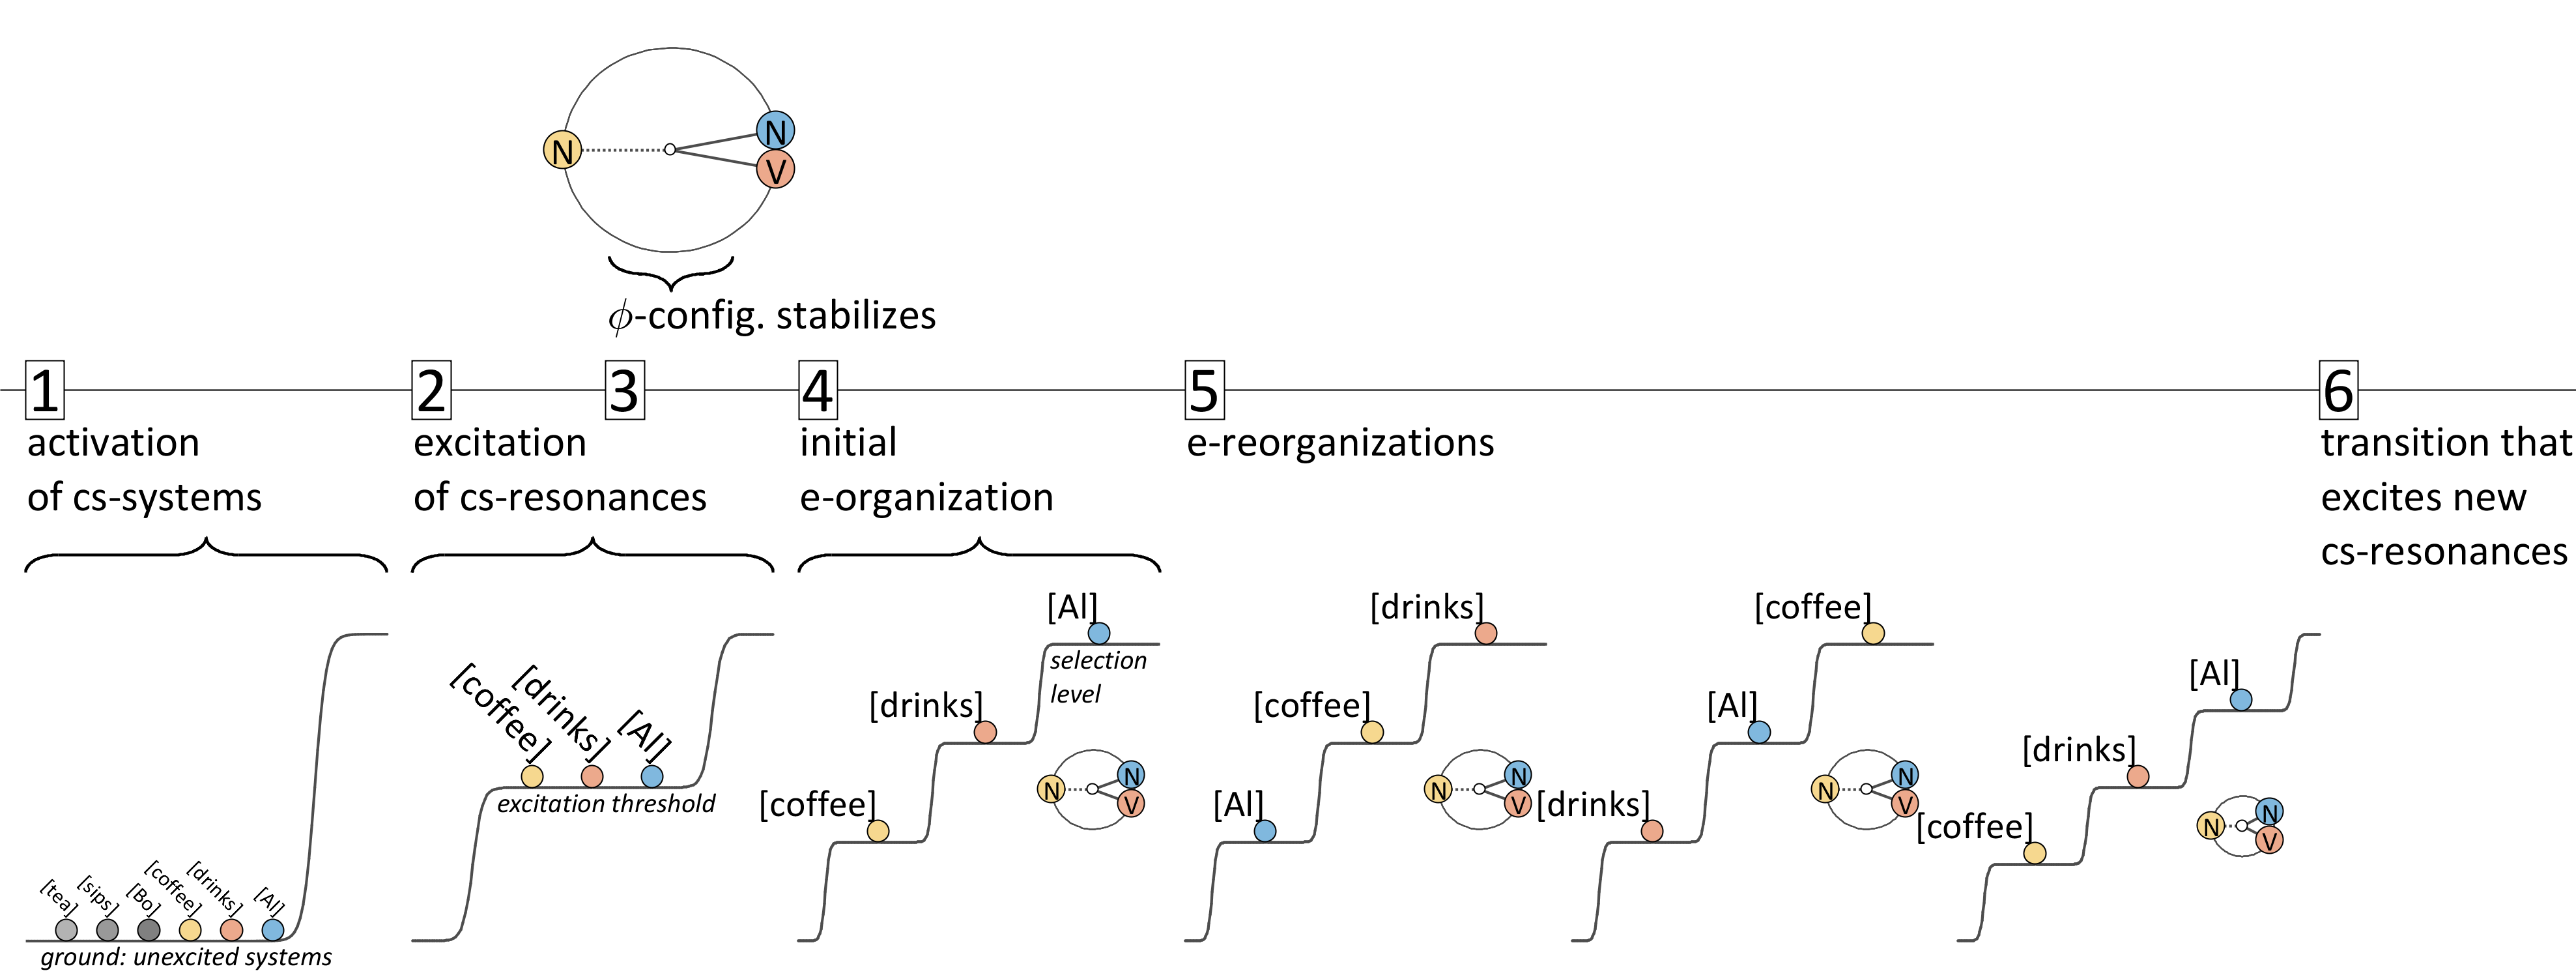
\includegraphics[width=\textwidth]{figures/Tilsen-img51.png}
\caption{\missingcaption}
\label{fig:4:1}
\end{figure}
 

\subsection{{1. Forces from the surroundings activate cs-systems}} 

The surroundings activate c-systems [Al], [drinks], and [coffee]. In general, other c-systems will already be active, or may become active. There may be many such systems, e.g. [Bo], [sips], [tea], etc. All of these c-systems begin to resonate with s-systems, forming cs-systems, but in the canonical trajectory we assume the \textit{e} values of these cs-systems are initially below the excitation threshold, i.e. unexcited. Recall the distinction between the ground-level (i.e. active, unexcited) and above-ground (excited) \textit{e} states of cs-systems: systems in the excited state can participate in stable φ configurations, while unexcited systems cannot. In the initial state of the canonical trajectory, all systems are unexcited, and hence shown on the ground level of the e-potential. This does not imply that all cs-system \textit{e} values are the same, merely that we have chosen not to differentiate them. Note that in more general cases, we do not need to assume that all systems are unexcited in the initial condition.

\subsection{2. Excitation of cs-resonances}

In the pre-stable phase of production, there is a competition process, or attentional focusing mechanism, which results in some cs-systems becoming excited and others remaining unexcited, or potentially deactivating. In the present example, [Al]\{+N\}, [drinks]\{V\}, and [coffee]\{-N\} systems become excited; [Bo]\{+N\}, [sips]\{V\}, and [tea]\{-N\} deactivate. The competitive character of the mechanism is due to interference between cs-resonances. For example, as pictured below, early on in competition process \{V\} resonates with both [drinks] and [sips] c-systems. All three of these systems (i.e. [drinks], [sips], \{V\}) have some initial θ and $\theta ′$. The initial phase velocities (or more relevantly, the short-timescale averages of $\theta ′$) are not necessarily equal, partly because the intrinsic frequencies of systems are not necessarily equal, and partly because the surroundings forces on each system can vary. Furthermore, the initial phases of these systems do not necessarily conform to proximal (φ=0) or distal (φ=π) relative phase patterns. In other words, the systems are neither frequency-locked nor phase-locked, prior to being excited. Thus we expect interference: φ{}-coupling of [drinks] and \{V\} interferes with φ{}-coupling between [sips] and \{V\}.

  
\begin{figure}
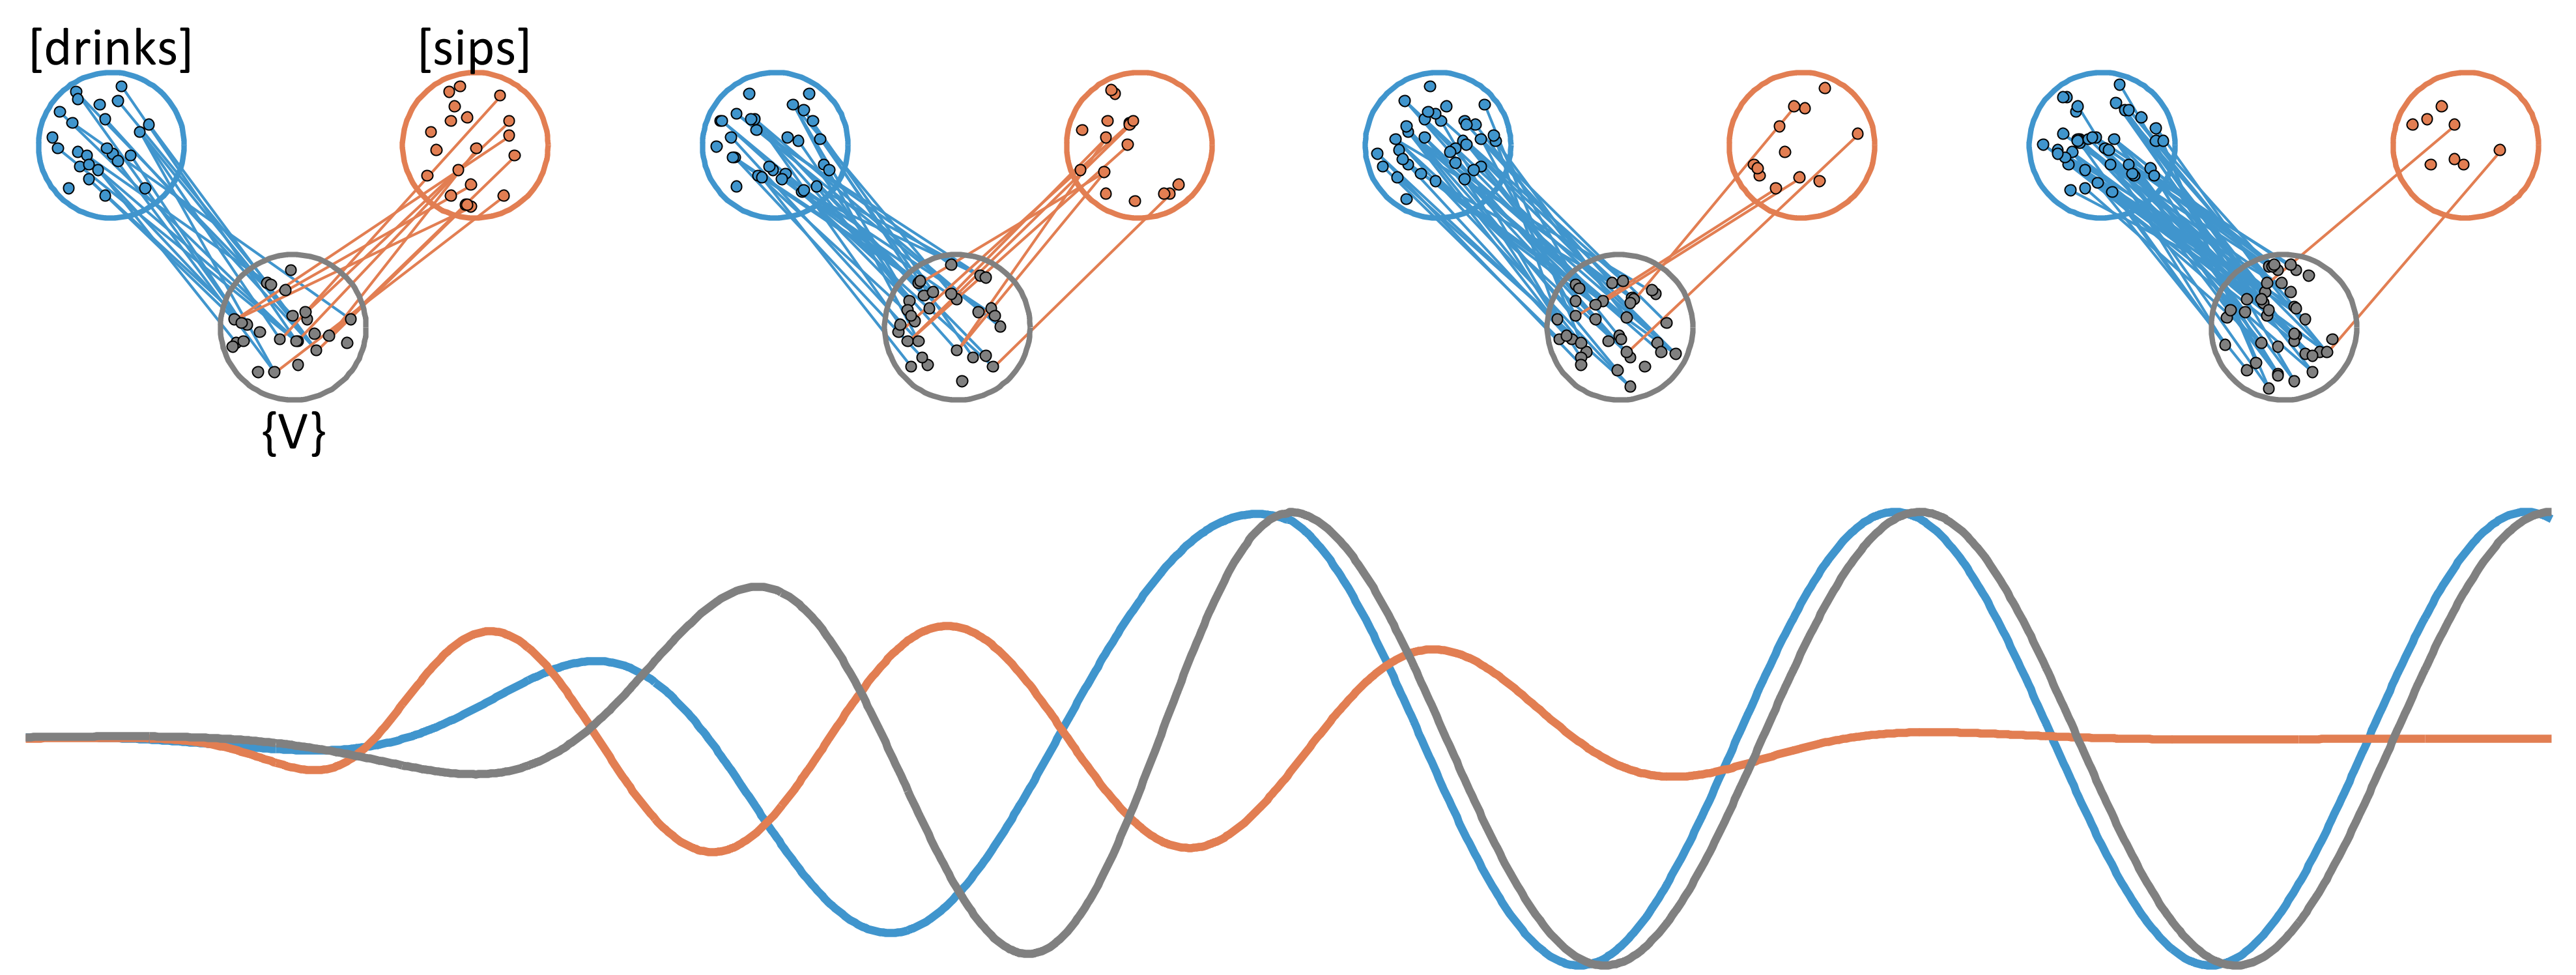
\includegraphics[width=\textwidth]{figures/Tilsen-img52.png}
\caption{\missingcaption}
\label{fig:4:2}
\end{figure}
 

  From the microscopic model we infer that φ{}-coupling force strengths depend on system \textit{e} values: the more neurons which participate in a collective oscillation, the more synaptic projections there are from that population to other ones. Thus if [drinks] has a higher \textit{e} value than [tea], it will exert stronger forces on \{V\}. This results in a greater tendency toward equalization of phase velocity between \{V\} and [drinks], compared to \{V\} and [tea]. Through e-coupling, \{V\} and [drinks] will mutually augment one another more than \{V\} and [tea]. The positive feedback loop, i.e. resonance, leads to excitation of the [drinks]\{V\} system, at the expense of [sips]\{V\}. The cs-system [drinks]\{V\} evolves toward a strong constructive interference pattern, while [sips]\{V\} experiences destructive interference.

  The outcome of resonance-focusing must be a complex function of the states of the active systems and surroundings forces. We do not attempt to model this function, but rather assert that in the canonical trajectory, some subset of active systems becomes excited; in the current example these are [Al]\{+N\}, [drinks]\{V\}, and [coffee]\{-N\}. Later on we consider deviations from the canonical trajectory in which the competition process does not immediately result in excited cs-resonances, or in which the processes is interrupted by surroundings forces.

  Why does one particular configuration of cs-systems emerge as opposed to another? For example, why does a state with excited [Al]\{+N\} and [coffee]\{-N\} systems arise, as opposed to excited [coffee]\{+N\} and [Al]\{-N\} systems (i.e. \textit{coffee drinks Al})? We assume that early in the pre-stable phase, the unexpected [Al]\{-N\} and [coffee]\{+N\} resonances are active and compete with the expected ones. Part of the reason why the expected set wins the competition may be learned asymmetries in coupling forces: c-systems with greater degrees of animacy, like [Al], are biased to resonate with the \{+N\} system, and c-systems with less animacy, like [coffee], are biased to resonate with the \{-N\} system. But learned semantic biases cannot be the whole story, since we must account for cs-resonance asymmetries in utterances such as \textit{Al sees Bo} where c-system animacies are the same. Thus we presume that information in the patterns of forces from the surroundings (i.e. sensorimotor experience) biases cs-coupling in a contextually appropriate way. For \textit{Al sees Bo}, the φ symmetry with respect to [sees]\{V\} of [Al]\{N\} and [Bo]\{N\} is broken by surroundings forces: asymmetries in how a producer experiences sensory information, e.g. aspects of the visual scene of Al seeing Bo which differ from aspects of the visual scene of Bo seeing Al, exert biases on c-system to s-system mappings in the pre-stable phase.

\subsection{3. Emergence of a stable φ configuration}

A φ configuration stabilizes due to strong φ{}-coupling forces between s-systems. φ{}-stabilization must follow excitation of the participating cs-resonances. This constraint follows from our hypothesis that cs-systems must be in the excited state in order to φ-couple strongly with other systems. The criterial/threshold \textit{e} value for excitation can be viewed as a minimal degree of order in a system which is necessary for a person to \textit{be consciously aware} of the system, an \textit{attentional threshold}, in a sense. Exactly what is meant phenomenologically by “awareness” and “attention” here, we do not attempt to elaborate. 

   Stabilization of a φ configuration is the beginning of a relational meaning experience, and in the canonical case the configuration will persist throughout the utterance. There a number of interesting questions to consider regarding meaning experience conceptualized in this way. How long must a stable φ configuration persist in order to give rise to awareness of a relational meaning? It seems reasonable to guess that in order for awareness to arise, the configuration must be maintained for a period on the order of 100s of milliseconds, but perhaps there are also circumstances in which we engage φ configurations on the order of 10s of milliseconds and of which we are not consciously aware.

  Can a relational meaning experience arise “by accident,” i.e. as a coincidence, without resulting from s-system φ-coupling? Coincidental relational meaning is a logical possibility. For example, surroundings forces may excite [Al]\{N\} and [drinks]\{V\} systems and \textit{by chance} (i.e. not through coupling of \{+N\} and \{V\}) the φ of [Al] and [drinks] could be approximately 0 or π, and the difference between their $\theta ′$ could be small. In that case, [Al] and [drinks] obtain the φ-pattern associated with agent-verb relational meaning, without having achieved this state through s-system coupling. Despite being a logical possibility, coincidental φ configurations are both unstable and highly improbable. If the intrinsic frequencies of the systems differ, their φ will wander in the absence of coupling. Even if we assume equivalent intrinsic frequencies, if we were to randomly draw the θ of two systems from uniform distributions, the likelihood that φ would be approximately 0 or π is very low. It is even less likely that φ would remain stable, because minor perturbations of $\theta ′$ from surroundings fluctuations or from the influences of other systems will alter any φ-pattern which has arisen by chance. Thus s-systems play a necessary role in stabilizing φ configurations.

\subsection{4. Emergence of a stable e configuration}

Excitation of cs-resonances necessarily precedes stabilization of φ configurations, but does φ configuration stabilization necessarily precede e configuration stabilization? In the canonical trajectory we stipulate that the e configuration stabilizes \textit{after} φ-stabilization. This is a sensible hypothesis because e configurations can depend on φ configurations. The mapping of cs-systems to e-potential levels varies substantially according to the freedom of word order in a language: in some languages, e-organization is strongly influenced by φ configuration. In languages with relatively free word order, the effects of surroundings forces on \textit{e} may have a greater influence on e-organization than learned φ-e mappings. We discuss differences between fixed and  free word order in more detail later on, but note here that e-organization is in general determined both by surroundings forces and learned φ-e mappings.

  The primacy of φ-stabilization relative to e-stabilization is also a sensible assumption for the canonical trajectory because φ-epochs (periods of time in which a φ configuration is stable) typically span multiple e-epochs (periods of time in which an e configuration is stable). In the canonical trajectory, the initial organization mapping of the excitation operator Ê may depend on φ-states, but subsequent reorganization mappings do not. For more general trajectories, we allow for e- and φ- organization mechanisms to interact in pre-stable and post-stable phase of production, and hence we expect an interplay between φ and \textit{e} states. However, in canonical production φ and \textit{e} states can interact only in the pre-stable phase; during stable epochs of canonical production, φ and \textit{e} states have no influence on one another. 

\subsection{5. Iterated reorganization of e configuration}

After the emergence of a stable e configuration, what happens next depends on the configuration itself: if the most highly excited system is above the selection threshold, then feedback processes induce the application of the canonical reorganization mapping: the selected system is demoted and others are promoted. This mapping is iterated until all systems have been selected. In contrast, if the most highly excited system is initially below the selection threshold, no reorganization occurs. Thus we distinguish between production regimes which are \textit{selective} (i.e. selection occurs) and those which are \textit{non-selective}, as shown below. Note that we represent the non-selective case by leaving the highest level of the e-potential unoccupied. For the canonical trajectory, we assume the selective regime, and hence iterated reorganization which potentially drives overt production. 

  
\begin{figure}
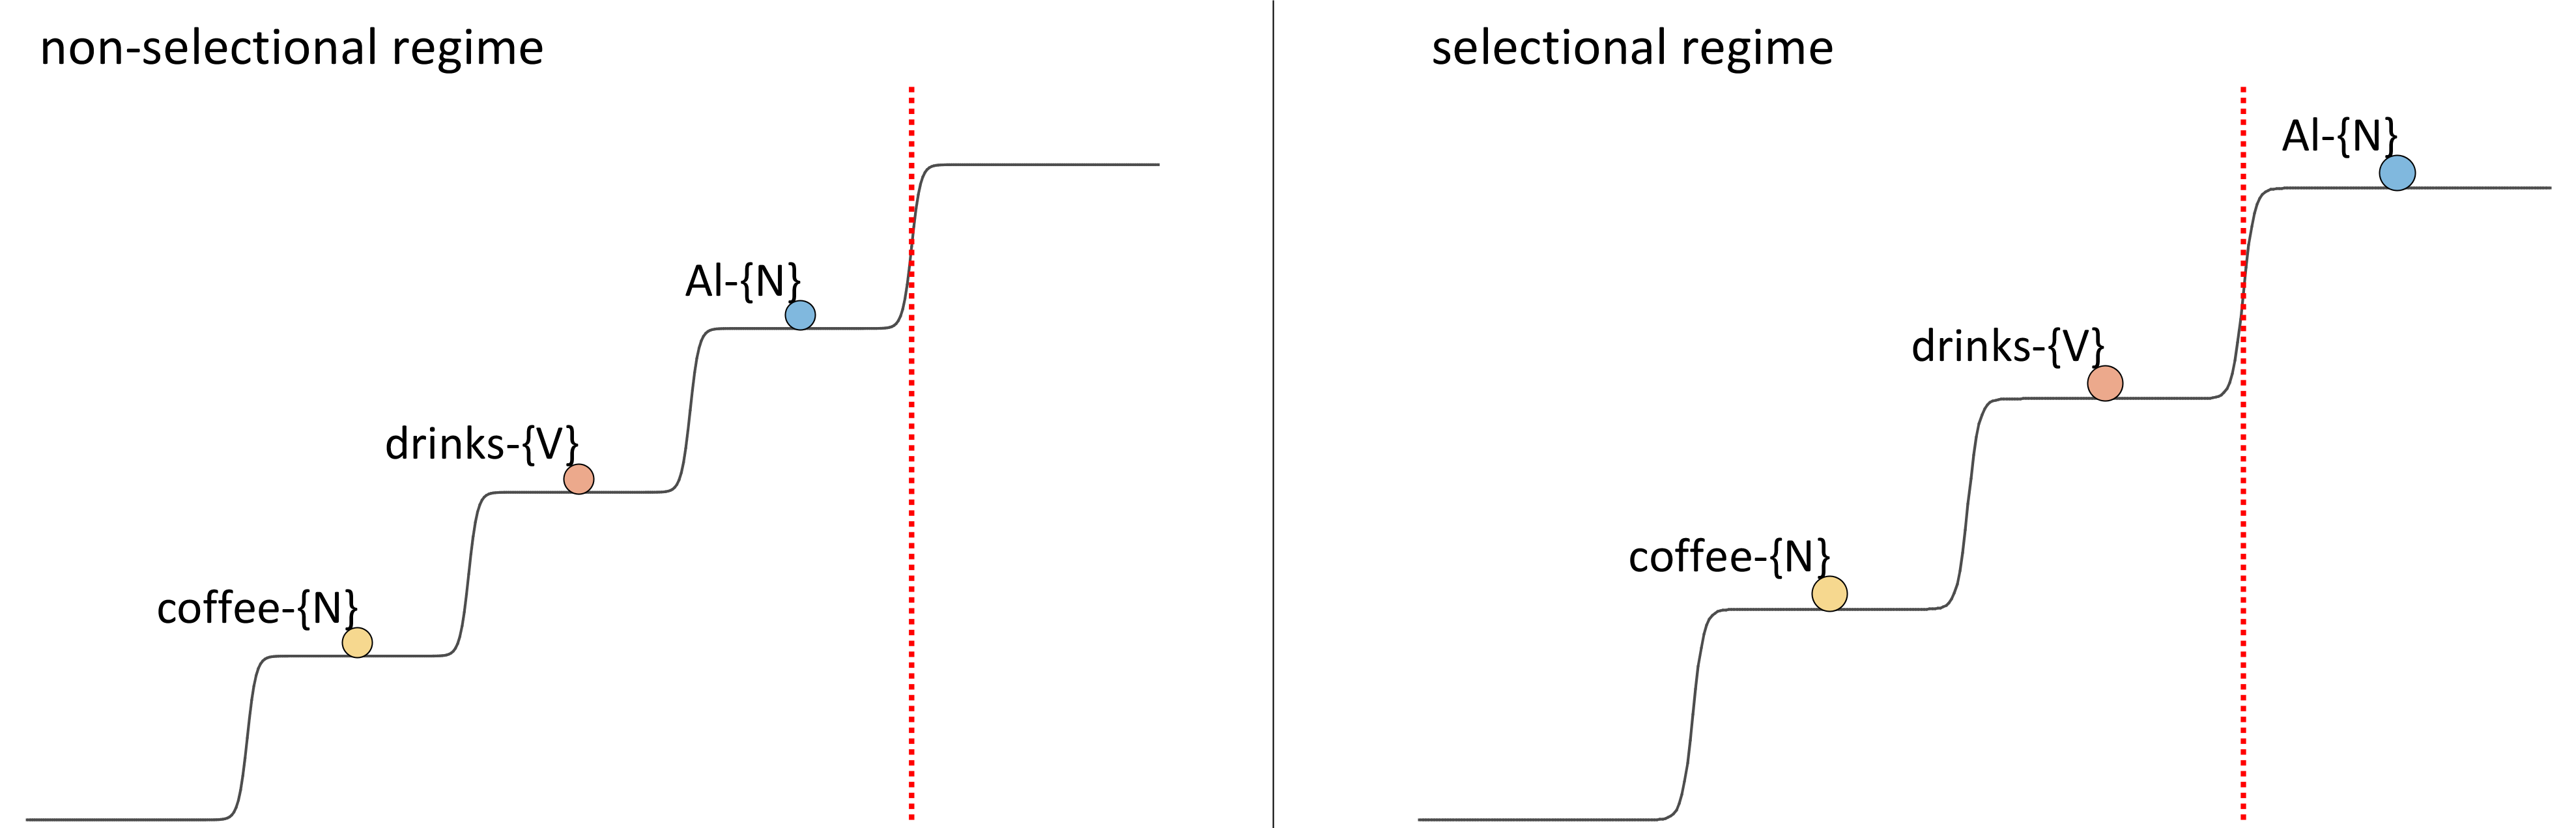
\includegraphics[width=\textwidth]{figures/Tilsen-img53.png}
\caption{\missingcaption}
\label{fig:4:3}
\end{figure}
 

  The selection threshold can vary over time. This variation could be quite complicated, because the threshold represents an integration of surroundings interactions with cs-systems. For example, a speaker can be in relatively higher and lower states of physiological arousal, more or less prone to engage in simulation or execution regimes of production. Alternatively, an individual can be in a regime where they direct attention to environmental stimuli, where motor sequencing must be inhibited. Thus the dynamics of the threshold are associated with an \textit{intention} to engage conceptual-syntactic simulation, and this intention is a function of many systems. Note that we use the term \textit{selection} to refer to a non-linear gating mechanism which depends on \textit{e} values and the selection threshold. This gating mechanism controls the selection of cs-systems.

  What causes Ê to transition from the stabilizing regime to the reorganization regime in the canonical trajectory? To answer this we introduce the \textit{parallel domains} hypothesis\footnote{This hypothesis is named in honor of Jean-Roger Vernaud, who believed deeply in the necessity of developing a unified understanding of syntactic and phonological patterns (see e.g. \citealt{FreidinVergnaud2001,Vergnaud1977}); I was the lucky beneficiary of a seminar Jean-Roger and Louis Goldstein held on this topic in the fall of 2009.} , which holds that gestural-motoric organization occurs through the same mechanisms as conceptual-syntactic organization: gestural systems resonate with motoric systems, motoric systems are strongly φ-coupled attractively or repulsively, and \textit{gm-systems} are organized into a quantal relative excitation potential. Furthermore, there are strong interactions between systems in conceptual/syntactic and gestural/motoric domains: activation of a cs-system activates associated gm-systems; excitation of a cs-system augments the \textit{e} values of those active gm-systems; selection of a cs-system induces excitation of the associated gm-systems, which in the canonical trajectory leads to selection of those gm-systems. More specifically, we imagine that the selection of a cs-system induces a nonlinear boost in the excitation of the c-system; the c-system is presumed to be +e-coupled to a \textit{g-domain}, a set of g-systems. The g-domain is thereby excited and selected. Feedback from gm-states then induces the transition to the reorganization regime of  Ê.

  In the parallel domains hypothesis, articulatory gestures (\textit{g-systems}) are analogs of c-systems, and motoric systems (\textit{m-systems}) are analogs of s-systems. The interaction between domains is such that selection of cs-systems drives organization of gm-systems, and this creates states which through feedback induce reorganization of cs-systems. The interactions between domains are schematized below. Activation of gm-systems precedes and is distinct from excitation of gm-systems. In the canonical trajectory, only the gm-domains of selected cs-systems are necessarily excited. Feedback regarding the achievement of a gm-state induces reorganization of cs-systems, which in turn leads to a new gm-organization and more feedback, etc.

  
\begin{figure}
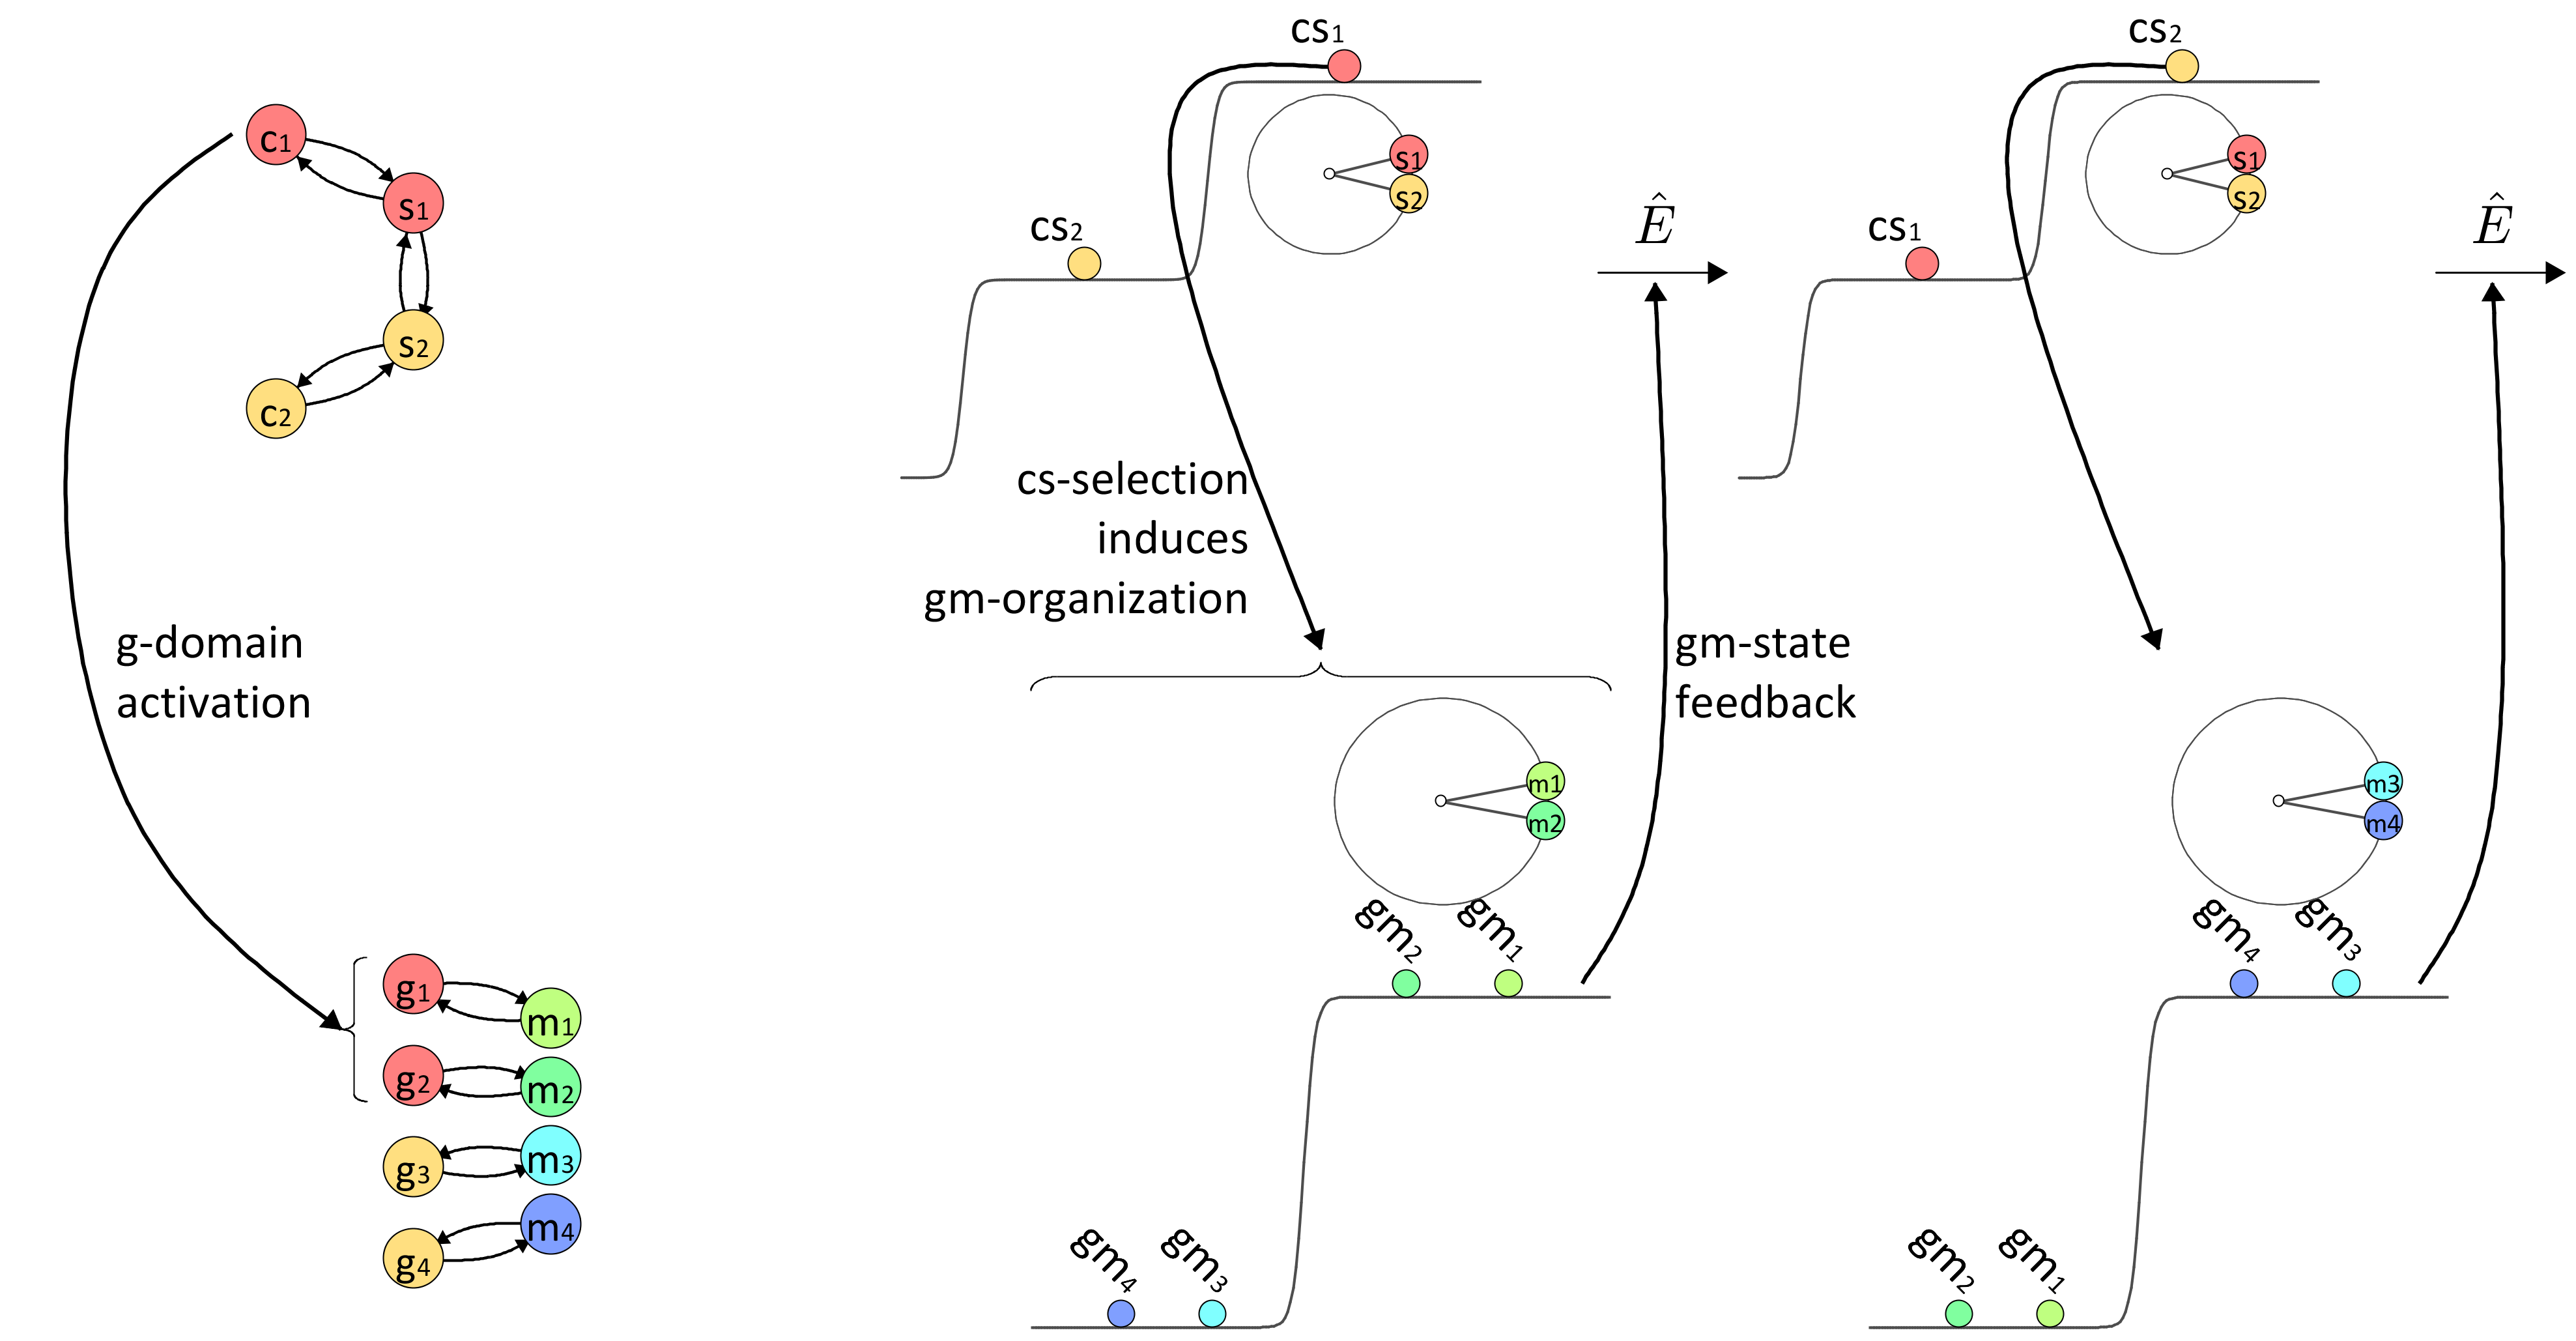
\includegraphics[width=\textwidth]{figures/Tilsen-img54.png}
\caption{\missingcaption}
\label{fig:4:4}
\end{figure}
 

  A specific example is shown below (for expository purposes we substitute \textit{Alexi} for \textit{Al}). When [Alexi]\{N\} is selected (A), the g-systems associated with \textit{Alexi} resonate with m-systems and gm-systems become excited (A\textsubscript{1}). The particular φ/e-organization that arises is partly learned (lexically driven) and partly influenced by “post-lexical” phonological processes (e.g. resyllabification). Note that in the depiction of gm-system e-organization, the gm-systems associated with each syllable occupy a different level. Here we use segmental labels for gm-systems out of convenience but a more useful analysis would depict gestures (i.e. bilabial closure, glottal adduction, etc., which are possibly the smallest scale of organization in premotor cortex). In a canonical trajectory, the most highly excited set of gm-systems is above the selection threshold, and this de-gates the execution of movements associated with the relevant g-systems. The precise timing of execution of co-selected gm-systems is determined by the relative phases and frequencies of those gm-systems (i.e. coordinative control, as described in Selection-coordination theory, cf. \citealt{Tilsen2016,Tilsen2018}). 

  
\begin{figure}
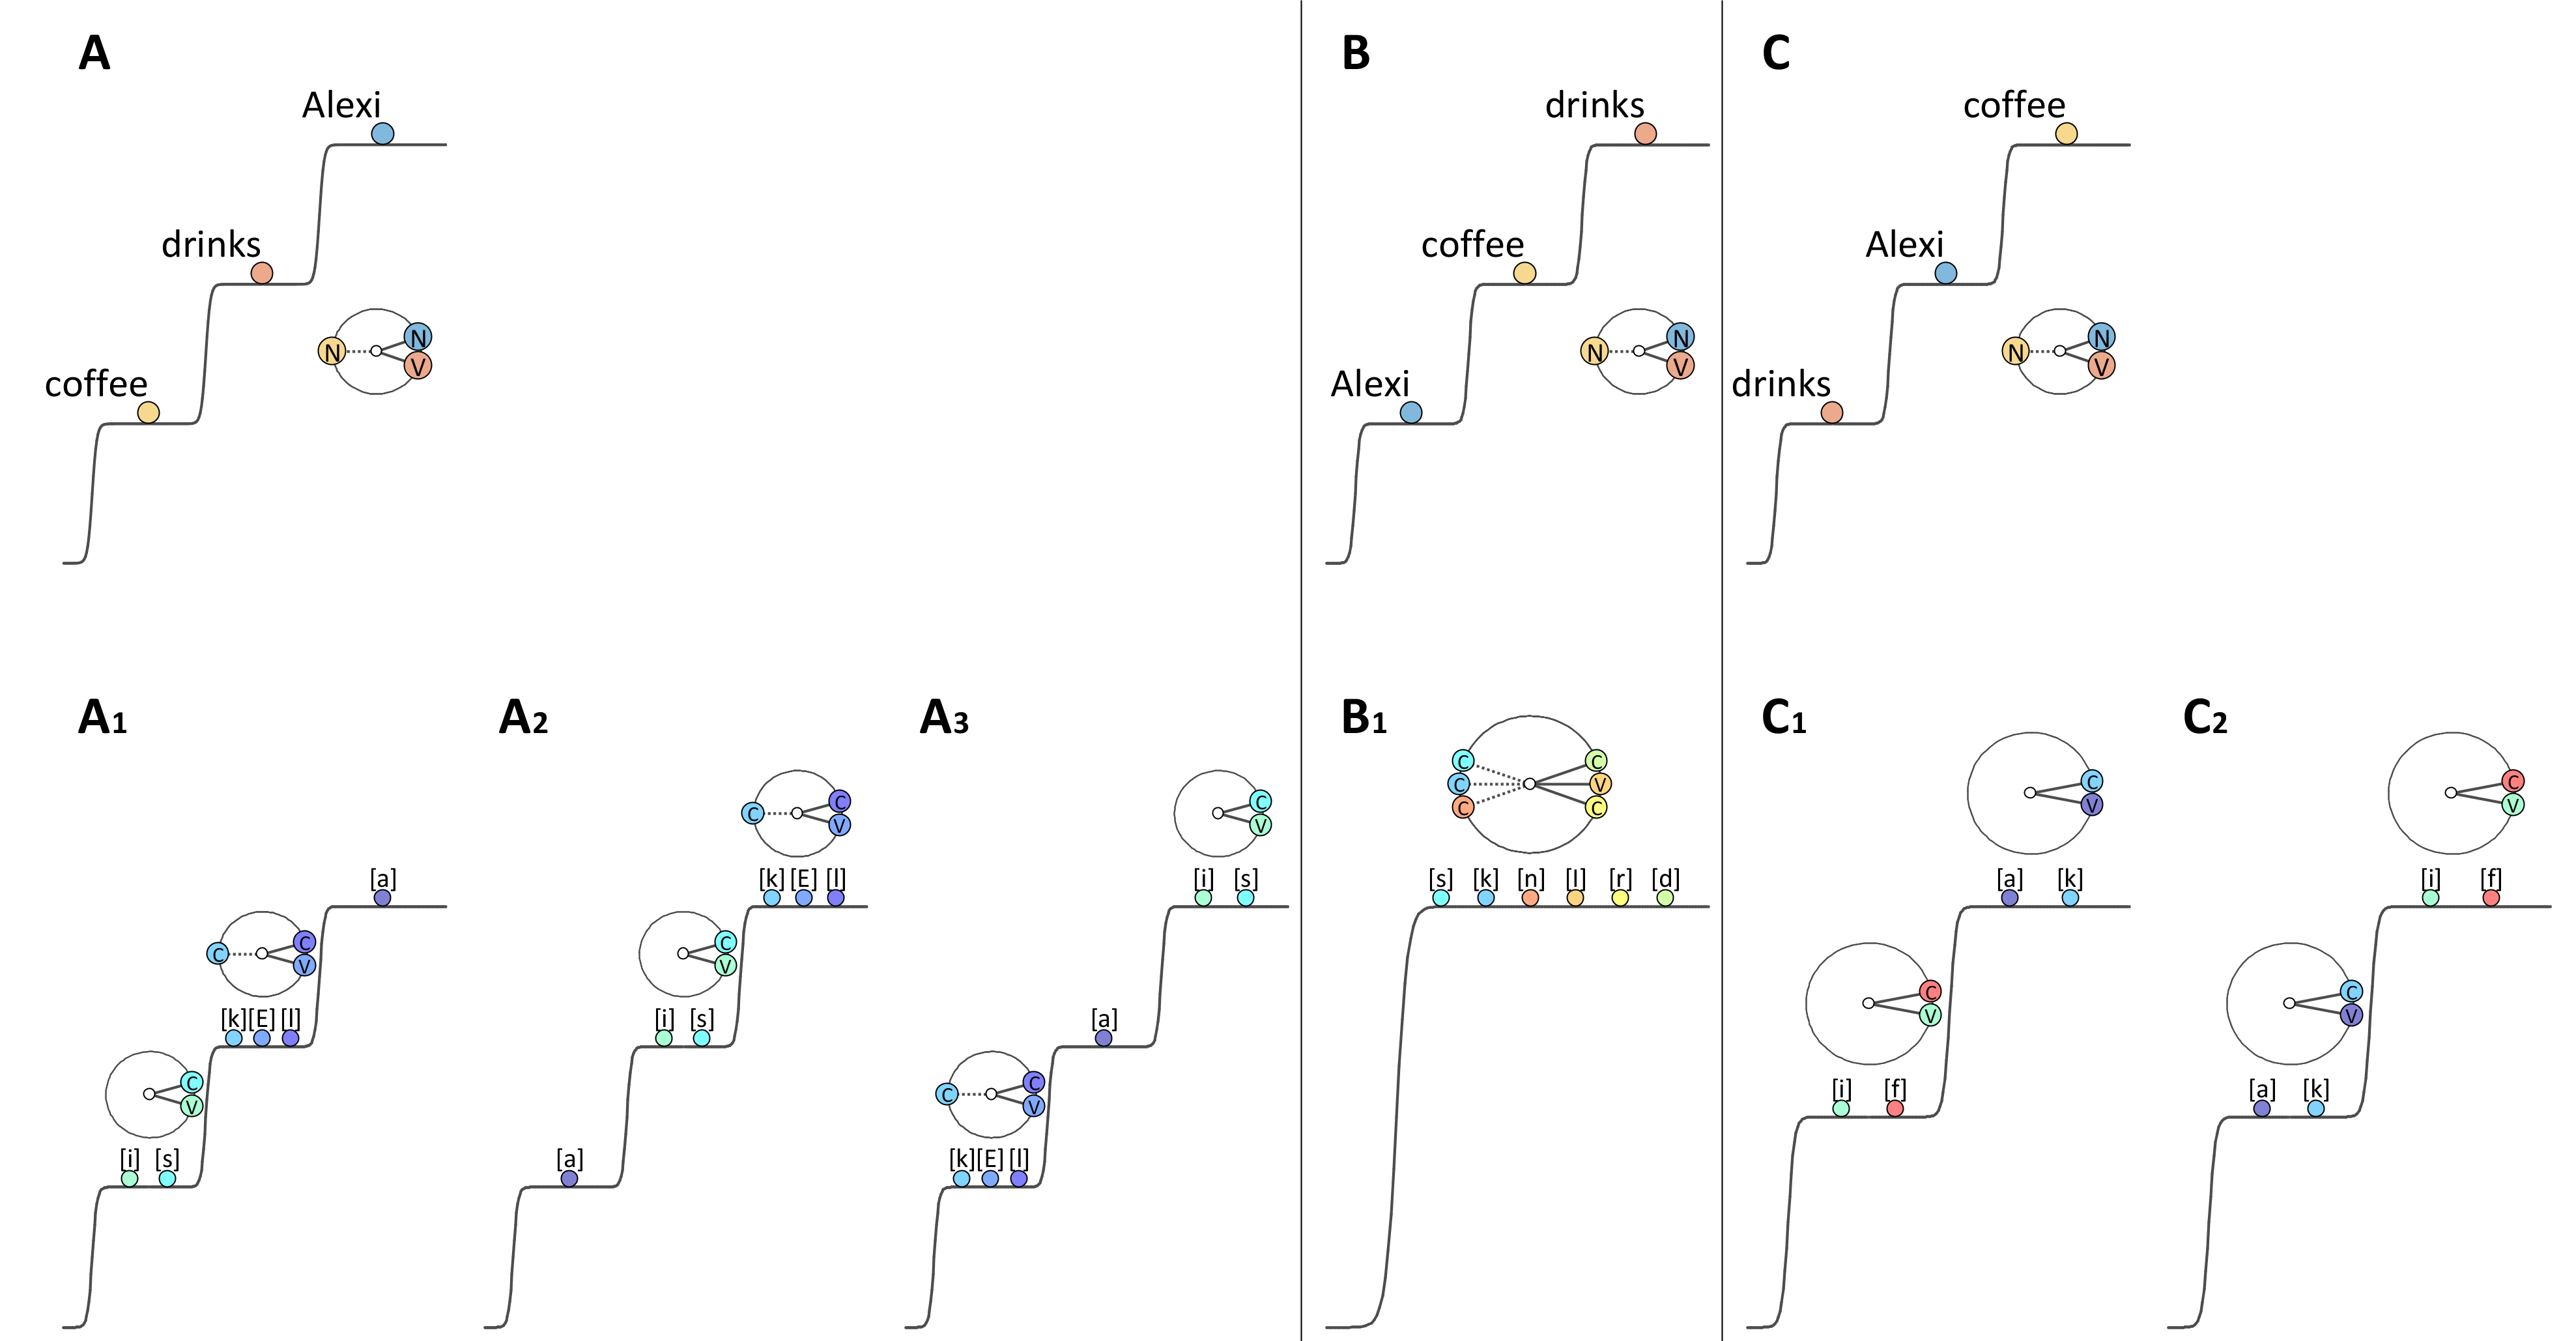
\includegraphics[width=\textwidth]{figures/Tilsen-img55.png}
\caption{\missingcaption}
\label{fig:4:5}
\end{figure}
 

  For adult speakers in normal circumstances, internal (i.e. predictive/anticipatory) feedback regarding achievement of articulatory targets leads to promotion of non-selected gm-systems and suppression of the selected set of systems (A\textsubscript{2}). The newly selected set is executed, internal feedback induces degating and suppression, leading to the gm-state in (A\textsubscript{3}). When all sets have been selected and suppressed, feedback regarding the gm-state associated with [Alexi] induces reorganization to the cs-state in (B), i.e. demotion of [Alexi]\{N\} and promotion of [drinks]\{V\}. When [drinks]\{V\} is selected, the g-domain of [drinks] is e-organized and executed (B\textsubscript{1}). Feedback leads to the s-system reorganization in (C), which leads to organization and reorganization of the gm-domain of [coffee] (C\textsubscript{1} and C\textsubscript{2}).

\subsection{6. The surroundings drive the system to a new state}

The φ-epoch in which [Al]\{+N\}, [drinks]\{V\}, and [coffee]\{-N\} are excited comes to an end. The state trajectory will change drastically, depending sensitively on the surroundings and other c-systems. Hence we make no assumptions about the subsequent state in the canonical production trajectory. We imagine that excitation of [Al], [drinks], and [coffee] c-systems may activate (“prime”) semantically associated c-systems through weak e-coupling. This priming comes in the form of biasing forces on the state trajectory, with numerous other surroundings forces determining the outcome. It is important to note that our representations depict only the most strongly excited (above-ground) systems, only the tip of an iceberg. In a more detailed analysis, many more cs-systems and gm-systems would be active throughout the trajectory. Various environmental/contextual factors—is it a socially appropriate time to speak?, are there salient environmental forces acting on a speaker?—along with the current system state, influence the evolution of the system. 

\section{Interactions between conceptual-syntactic and gestural-motoric organization}
\rohead{Conceptual-syntactic and gestural-motoric organization}

The o/el framework aims to provide a \textit{comprehensive} framework for analysis of language, a theory that can describe any empirical phenomenon. Our primary focus in this book is on conceptual-syntactic organization, rather than gestural-motoric organization. However, there are a number of hypotheses regarding gestural-motor organization and its interaction with conceptual-syntactic organization, which are worth discussing here.

\subsection{Similarities between relational meaning and temporal coordination}

One deep consequence of the parallel domains hypothesis is that two superficially distinct phenomena—relational meaning and precision control of movement execution—arise from the same mechanism. The principle of relational meaning corresponds to a principle of gestural coordination. Specifically this shared mechanism is φ-coupling between syntactic systems and between motoric systems, which indirectly brings about a φ configuration between conceptual and gestural systems, respectively. Distinctions such as agent/patient (\{+N\}, \{-N\}) and onset/coda (\{+C\}, \{-C\}) are analogous, since agents and onsets experience +φ (attractive) forces from \{V\} and vowels, while patients and codas experience -φ (repulsive) forces from \{V\} and vowels. This speaks to a deep connection between our experience of meaning and coordination of movement. The need to flexibly coordinate a fairly small set of movements is an evolutionarily ancient problem, while the need to flexibly relate a vast multitude of concepts is relatively more modern. Our ability to experience a wide variety of relational meanings probably originates from duplication-induced redundancy and functional divergence in the neural systems that support φ-coupling of movement tasks. 

\subsection{Differences between syntactic and motoric sequencing} 

Although there are deep similarities between cs- and gm-organization, there are also some important differences: 

\begin{enumerate}
\item \textit{m-system} φ configuration\textit{al restriction}. Whereas s-system φ configurations can arise between systems which occupy different e-levels, m-system φ configurations tend to arise only for co-selected gm-systems, i.e. m-systems which occupy the same level. 

\item \textit{gm-interference is more stable than cs-interference}. Both c- and g- systems can interfere with other c- and g- systems, when resonating with the same s- and m- systems. However, gm-resonances appear to interfere with one another to a lesser extent. For instance, it is possible to have a stable configuration of three co-selected \{+C\} and \{-C\} constriction gestures, as in the word \textit{sprints}. In contrast, lexical s-systems like \{+N\}, \{-N\}, and \{V\} are never co-selected. This suggests that \{+C\} and \{-C\} differentiations of gm-systems which have similar \textit{e} values can be accomplished without destabilization. We note that the ability to organize multiple gm-differentiations of \{+C\} or \{-C\} systems must be learned, and many languages lack the complex syllable structures which require such differentiations.

\item \textit{c-system numerosity}. c-systems are vastly more numerous and diverse than g-systems. This is likely because g-systems interact more broadly with motor and sensory physiology. Practical considerations dictate that we construct c-systems in an analysis-specific way, because there are potentially so many of them. In contrast, we can often identify an constant set of g-systems for analyses of a given language (at least on supra-utterance scales), which is motivated  by articulatory and acoustic observations.

\item  \textit{Timescale of} φ \textit{configuration.} s-system φ configurations persist and remain stable over relatively longer periods of time than m-system φ configurations. In the cs domain, φ configurations tend to persist over multiple reorganizations of e configurations; in the gm domain, φ configurations tend to be associated with just one cs domain e-epoch.
\end{enumerate}

  Differences between syntactic and phonological patterns should be derivable from differences in cs- and gm-organization, such as those listed above. For example, the apparently greater degree of “non-locality” of conceptual relations vs. gestural relations may be a consequence of differences in configurational restrictions and relevant timescales. (Locality differences are not, of course, structural distances, because we do not conceptualize language as spatial ordering of objects in a linear space.) Differences between cs- and gm-organization should in turn be derivable from neurophysiological differences in the relevant neural populations.

\subsection{Thresholding for simulation and execution}

The hypothesized interaction between cs- and gm-domains involves three gating mechanisms,\footnote{A sensible pursuit in this context would be to associate the gating mechanisms/thresholds with neuro-behaviorally inspired inhibitory mechanisms \citep{DuqueEtAl2017,DuqueEtAl2010,%twice
,DuqueIvry2009,MayrEtAl2006}), but I have not attempted to explore this association in any detail.} which are associated with three thresholds: an s-selection threshold, an m-selection threshold, and an execution threshold. The states of these thresholds—which we call \textit{gates}—relative to the states of the relevant cs- and gm-systems, determines a \textit{production regime}, i.e. a class of state trajectories. 

  A threshold/gate should be viewed as an analytical simplification of forces which exhibit a nonlinear dependence on \textit{e} value. Each gate can be in a binary state: \textit{open} or \textit{closed}, where \textit{open} refers to any state in which \textit{e} values of relevant systems are below a threshold parameter value. If the states of all three gates are independent, there are 2\textsuperscript{3} = 8 distinct gate configurations. Alternatively, the gating mechanisms may be hierarchically organized, such that the highest closed gate determines the production regime; in that case there are only 4 distinct regimes. The {\figurebelow} labels the production regimes associated with a hierarchically organized interaction between gates.

  
\begin{figure}
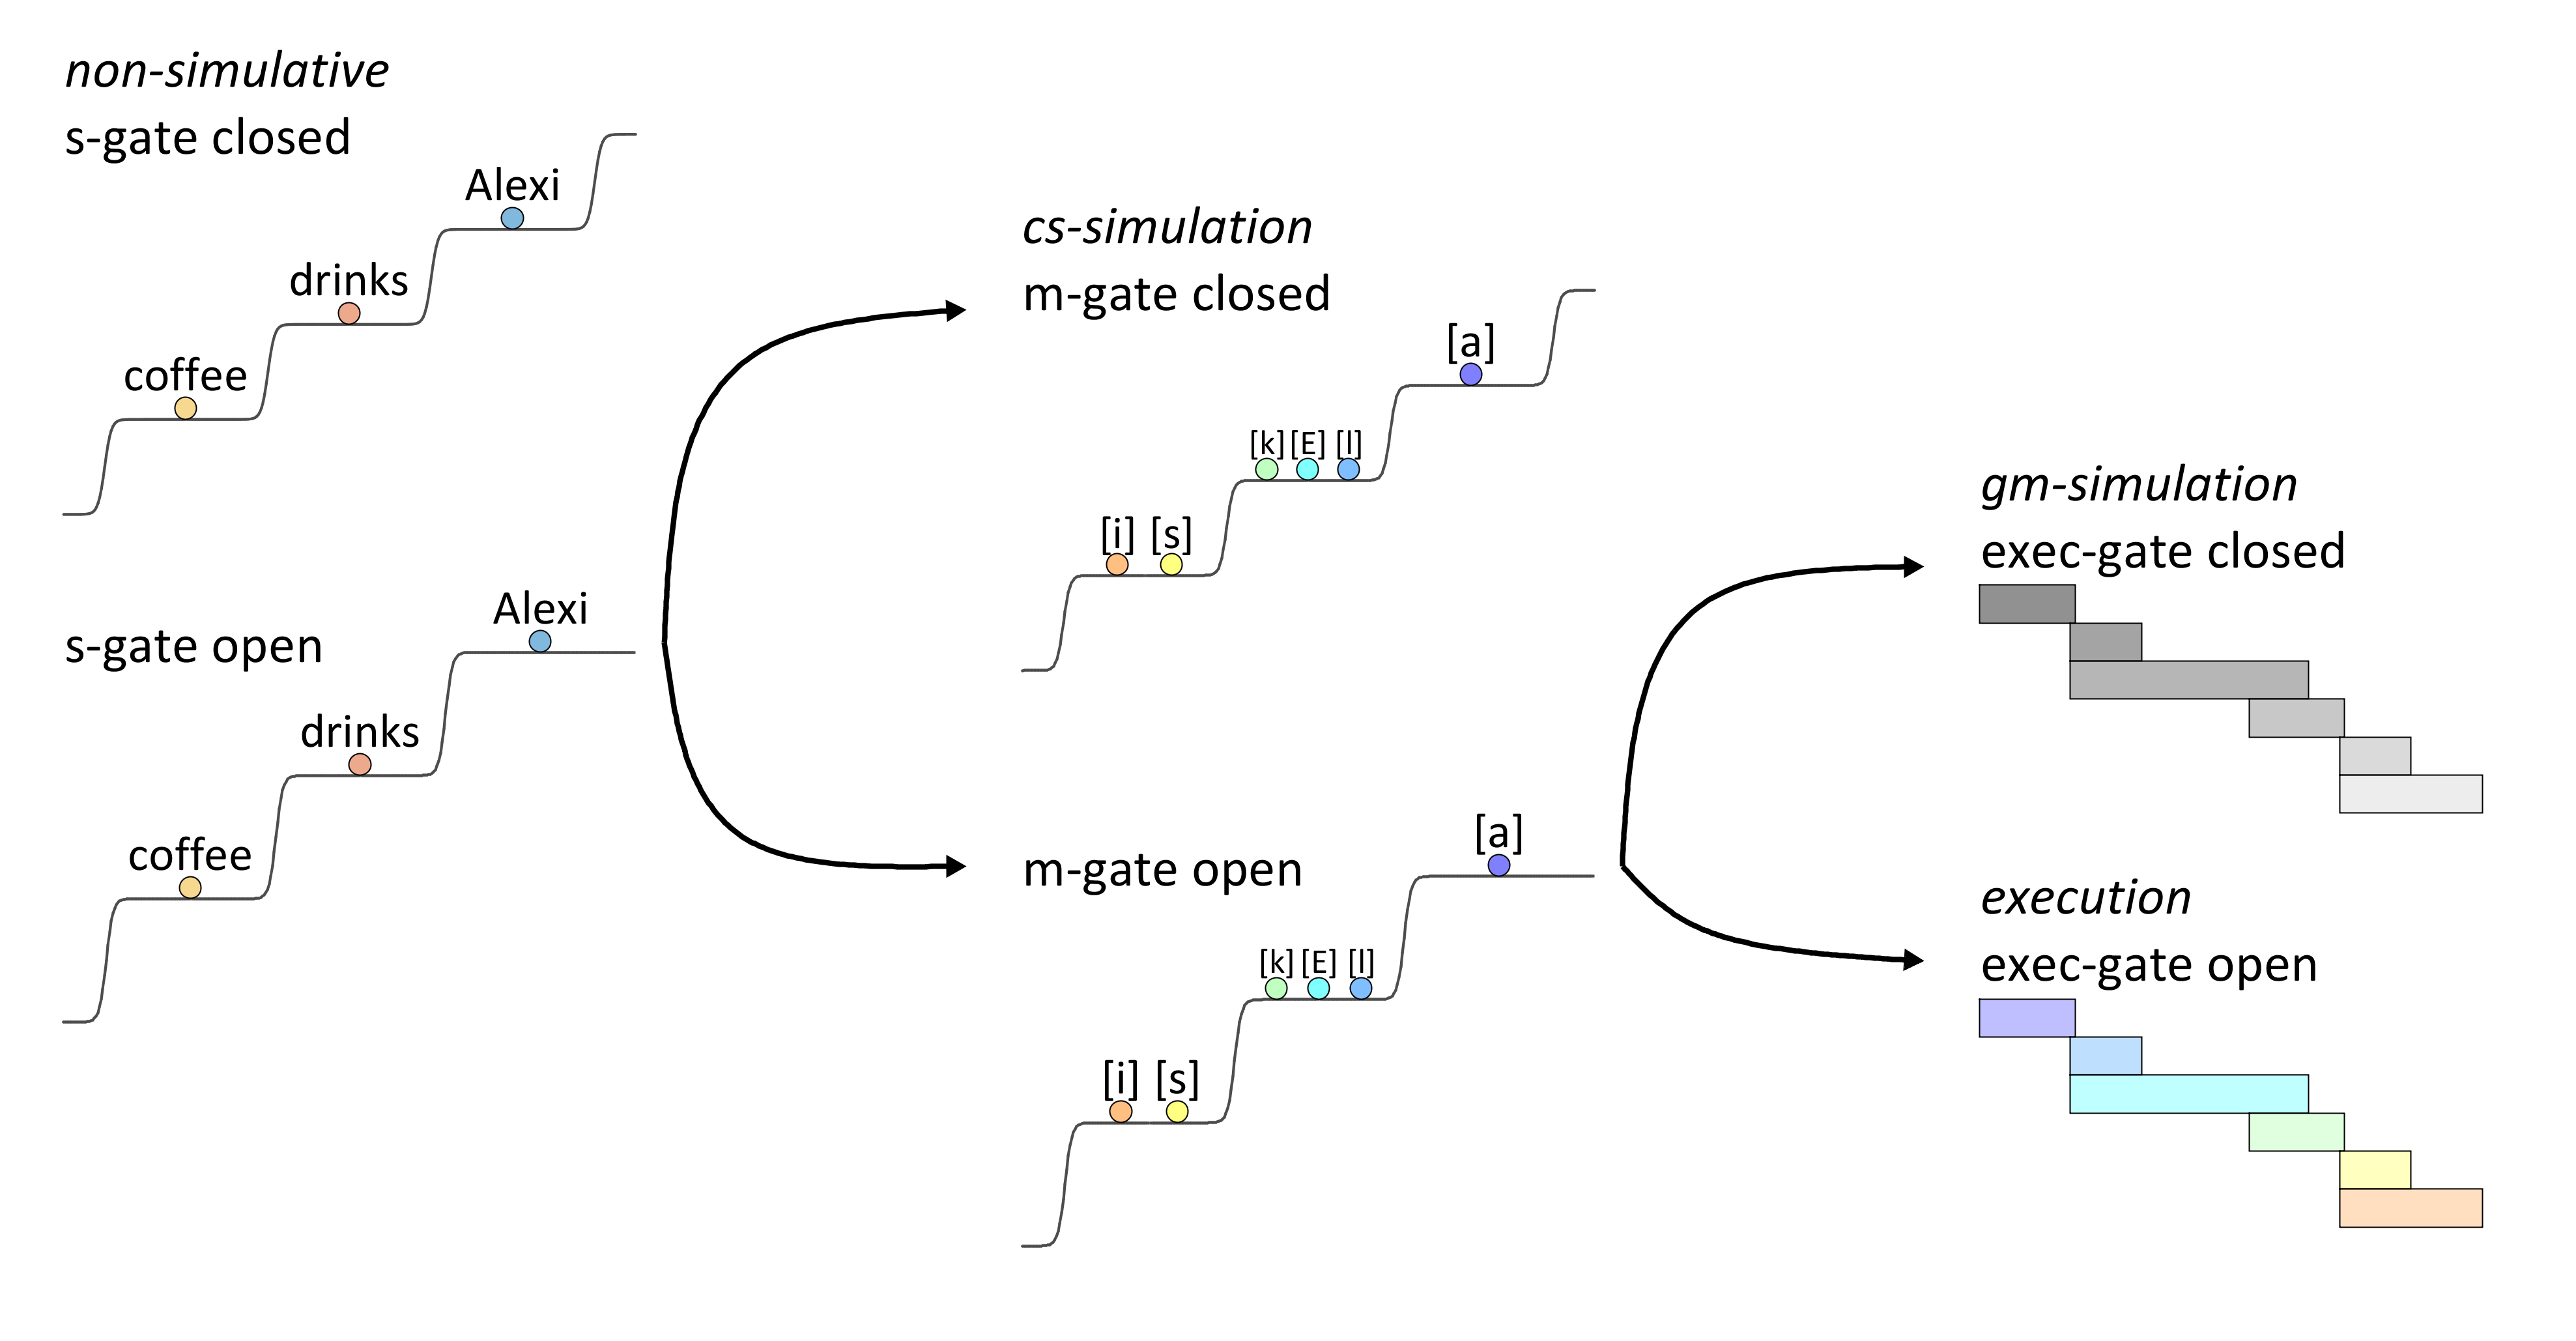
\includegraphics[width=\textwidth]{figures/Tilsen-img56.png}
\caption{\missingcaption}
\label{fig:4:6}
\end{figure}
 
\begin{enumerate}
\item \textit{non-simulative} regime: the s-system selection threshold (\textit{s-gate}) is closed. Relational meaning experiences can arise, but no cs-selection occurs. This regime may be associated with “non-verbal” thought. It is difficult to characterize what sorts of behaviors this regime is associated with, because there is by definition no verbal motor behavior that can be observed, without cs-selection. 

\item \textit{cs-simulation} regime: the s-gate is open, but the m-system selection threshold (\textit{m-gate}) is closed. Because the s-gate is open, highly excited s-systems can be selected, and this causes gm-resonances to be excited. s-system e configurations can be reorganized in the canonical way, driven by feedback. Yet because the m-gate is closed, motor commands are not generated and hence movements are not simulated. 

\item \textit{gm-simulation} regime: s- and m-gates are open,  but a global motor execution gate (\textit{exec-gate}) is closed. Motor commands and internal sensory feedback from movement are generated, but movements are not executed. We identify the gm-simulation regime with subvocal rehearsal and silent/covert speech. 

\item \textit{execution} regime: s-, m-, and exec-gates are open, overt speech can occur. More generally, verbal motor behaviors can arise: speaking, signing, handwriting, typing.
\end{enumerate}

  Do other production regimes occur, which could  be derived from non-hierarchical gate interactions? There are four possibilities. One is when the s-gate is closed but m- and exec-gates are open; this regime may be associated with behaviors such as filled pauses and floor holding, i.e. motor actions which are not necessarily driven by cs-resonances. Whether the remaining three possible combinations correspond to identifiable production regimes is unclear. It seems reasonable to infer that when m-gates are closed, no speech-related motor behaviors occur and exec-gate states are irrelevant to classification of production regimes.

\subsection{The roles of internal and external feedback in e configuration reorganization}

Reorganization of both cs and gm e configurations is driven by sensory feedback. We assume there are parallel feedback mechanisms for cs and gm states, and that these are associated with both internal and external feedback loops. There is a substantial literature based on the distinction between internal and external feedback when applied to motor control and speech (\citealt{Hickok2012,Kawato1999,MiallWolpert1996,RamanarayananEtAl2016,WolpertEtAl1995,WolpertKawato1998}); this distinction can be extended to higher levels of linguistic processing as well (\citealt{HagoortLevelt2009,Laver1973,Levelt1983,Levelt1989,Nooteboom1973,NooteboomQuené2008,Postma2000}).

  External feedback is sensory information regarding the state of the environment. The “environment” here is the physical state of the world: movement leads to changes in the state of the environment, e.g. in spatiotemporal acoustic energy distributions, articulator positions, muscle stretch, etc. These changes influence the states of various peripheral sensory systems, providing various forms of information, i.e. auditory, tactile, proprioceptive, etc. This information in turn influences the states of g-sensory systems, which we imagine are populations which integrate sensory information. In general, this external feedback can result in adjustments of motor commands, suppression of selected m-systems, and degating of subthreshold m-systems. However, a fairly long time delay exists between when movement occurs and when external sensory feedback associated with movement becomes available. This delay makes external sensory feedback relatively less useful for online control of movement, compared to internal feedback. 

  Internal sensory feedback is sensory information “predicted” by the nervous system, regarding the state of the environment. The prediction comes from an \textit{internal model}, which maps outgoing motor commands to sensory states. A so-called \textit{efference copy} of motor commands (or better, a motor state) is mapped to a representation of the anticipated sensory consequences those commands. Because of its anticipatory nature, internal feedback is useful for adjusting motor commands and reorganizing gm-system during execution. It is worth noting that “prediction” implies agency, and the nervous system is only metaphorically agentive. Thus it is more appropriate to describe internal feedback as follows: motor states induce sensory states, and these states are similar to ones that are induced a bit later via sensory information from the external environment.

The distinction between internal and external feedback is schematized below. In the gm-domain, internal feedback can lead to suppression (demotion) and/or degating (promotion) of systems \textit{before} external sensory feedback regarding target achievement has been received. Internal gm-feedback can also drive promotion and demotion of cs-systems in the cs-domain, via c-sensory systems. Thus internal feedback can be viewed as a general mechanism for influencing the timing of e-reorganization.

  
\begin{figure}
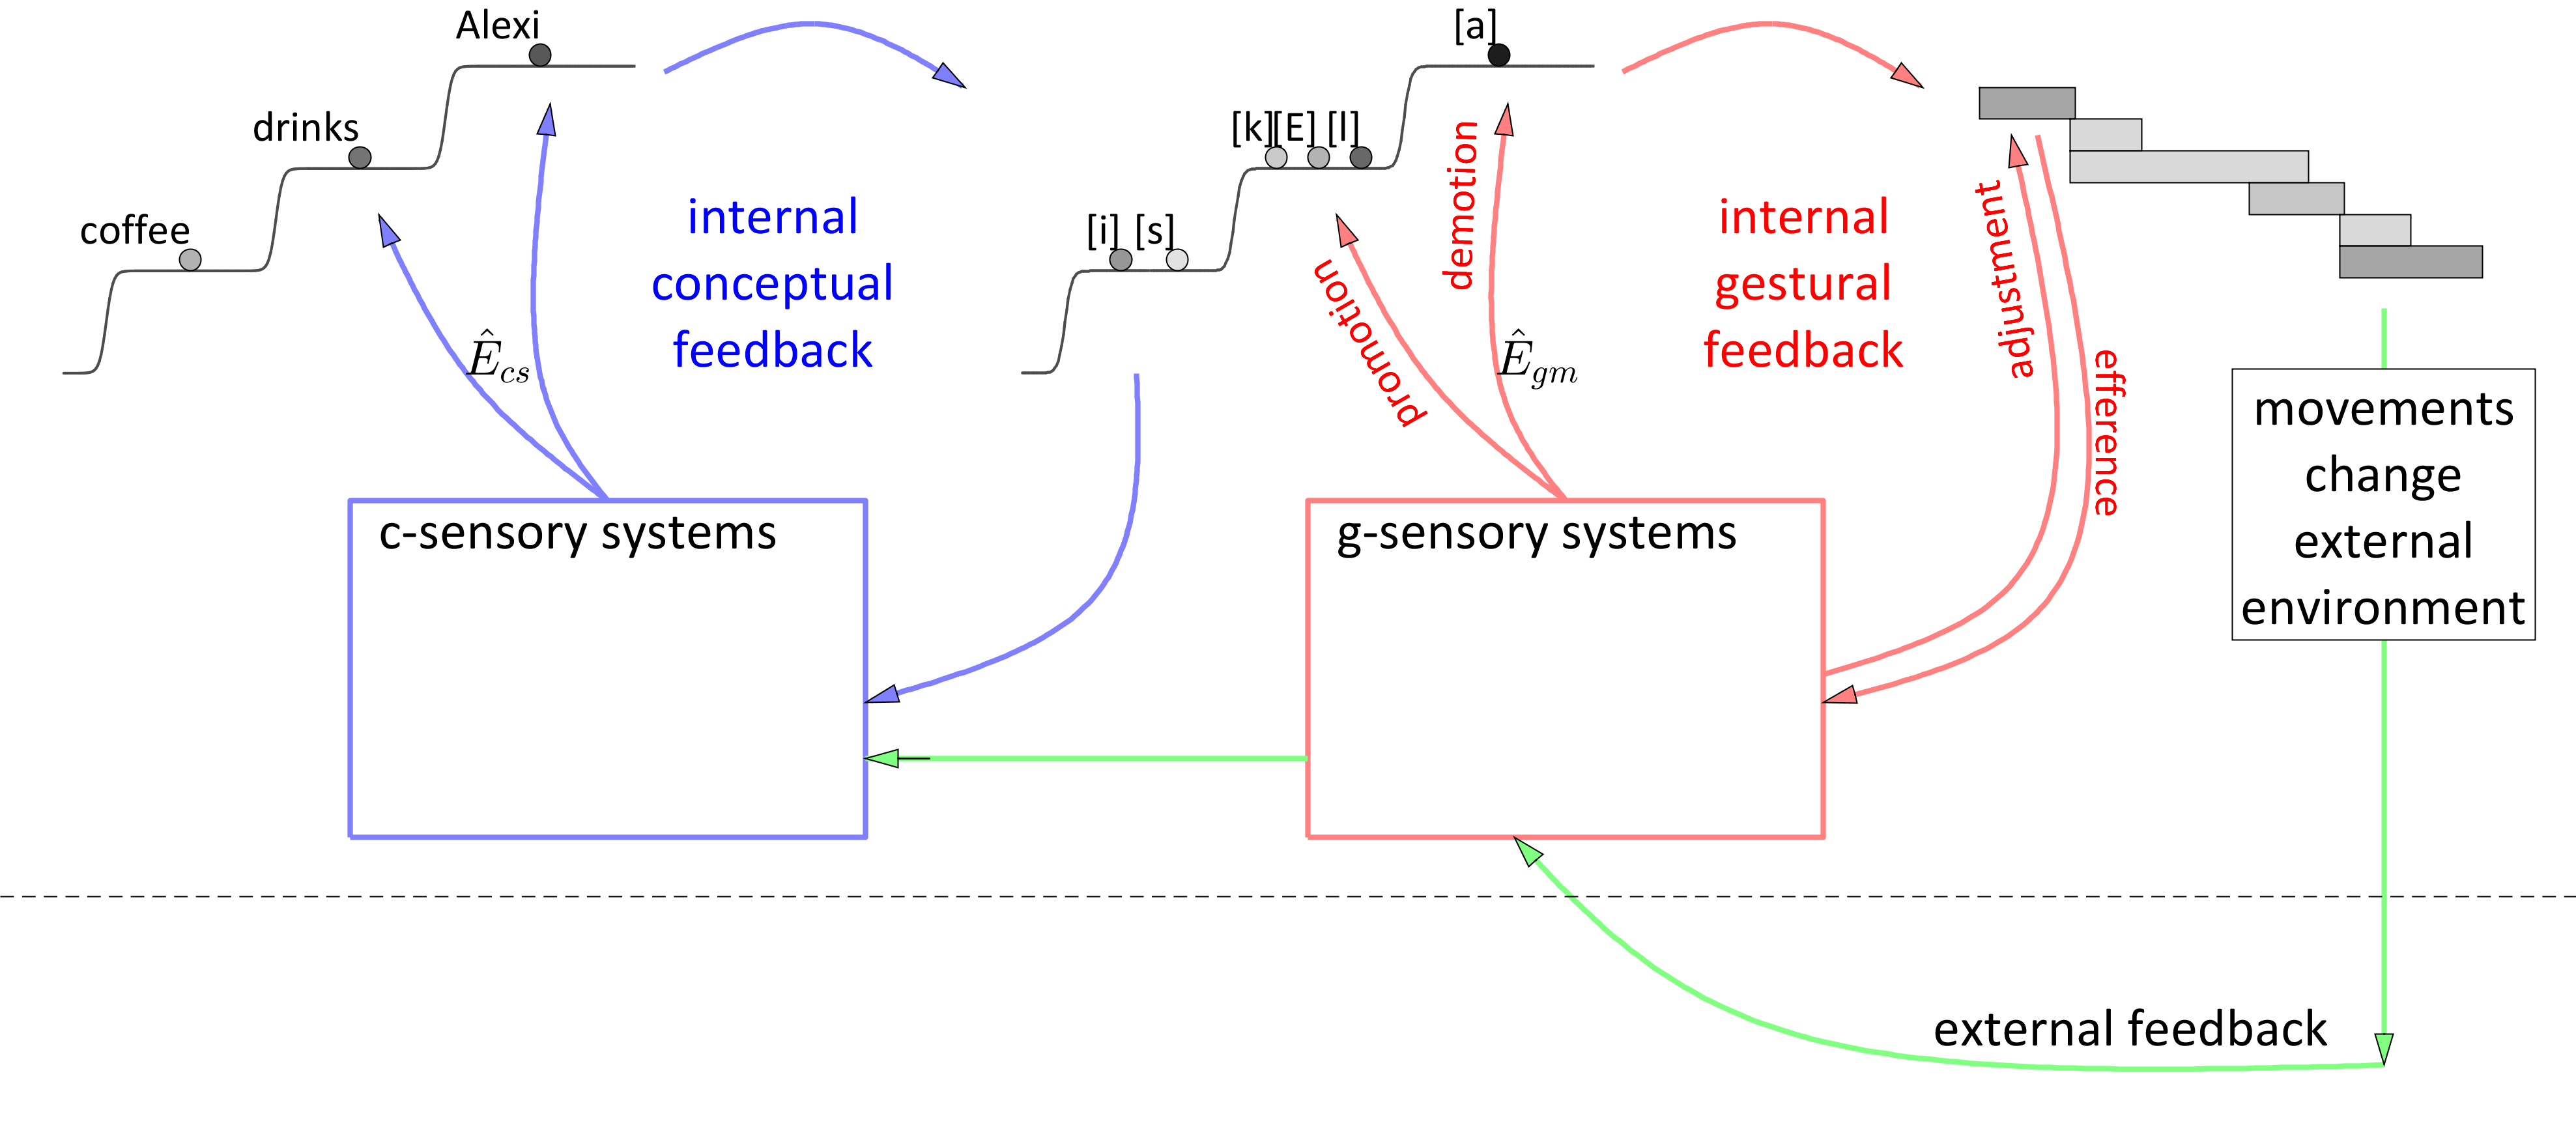
\includegraphics[width=\textwidth]{figures/Tilsen-img57.png}
\caption{\missingcaption}
\label{fig:4:7}
\end{figure}
       

  To what extent are internal and external feedback involved in cs- and gm- reorganization? The answer can depend on many factors. First, because internal models (which map motor states to expected sensory states) are learned, young children must rely on external feedback to a greater degree. This is consistent with the observations that young children speak more slowly and produce syntactically simpler utterances. Second, the relative influence of internal vs. external feedback must depend on a production regime, i.e. on threshold states. For example, when exec-gates are closed, as in motor simulation, no external sensory feedback is available. Hence internal feedback is the sole mechanism for driving e-reorganization in subvocal rehearsal. Third, environmental circumstances which induce mismatches between internal predictions and external feedback can induce greater reliance on external feedback. In sensory perturbation paradigms (e.g. speech in noise, spectrally altered auditory feedback, mechanical perturbation of movement), speakers often slow down and compensate for the alteration. These behaviors are presumably a consequence of detection of a mismatch between internal predictions and external information; when such mismatches are detected, the system can no longer rely on the accuracy of the prediction, and reverts to reliance on the external information. Fourth, various contextual forces may induce speakers to attend more or less closely to their own productions, resulting in varying degrees of reliance on external feedback.

\subsection{Disfluencies}

Abnormalities in trajectories of conceptual-syntactic and gestural-motoric systems can be understood by considering the ways in which interactions between φ/e-organization, thresholds, and feedback can deviate from those associated with the canonical production trajectory. These deviations predict a typology of disfluency/speech error mechanisms which differs from standard classifications (see \citealt{Fromkin1971,Fromkin1984,Shriberg2001}). To develop this typology we distinguish between (i) disfluency manifestations, (ii) disfluency mechanisms, and (iii) disfluency origins. Manifestations are observable abnormalities in production, whereas mechanisms are hypothesized deviations from the canonical trajectory which result in a disfluency manifestation. The origins of these deviations are surroundings forces and we have little to say about them—there are numerous possibilities for why a particular deviation occurs and we rarely have a solid basis for determining them. 

  The aim of constructing a disfluency typology is to map between mechanisms and manifestations, but this is complicated because the relation is not expected to be one-to-one. In particular, some classes of manifestation may arise from more than one mechanism. For example, there may be multiple abnormal cs-trajectories which converge to the same abnormal gm-trajectory. 

  Another complication is that the initial construction of what constitutes an abnormality must presuppose a canonical \textit{intended} or \textit{target} trajectory. We often assume that there was some utterance a speaker intended to produce, that something went wrong, and that the speaker produced something else. It may not be appropriate to impose these assumptions in many circumstances. In an empirical context, the implied target trajectory is always an analytical guess: we observe some manifestation(s) of disfluency, and based on our familiarity with language, our expectations, and our notions of similarity, we guess a target utterance.

  Lets consider an example. Imagine that a speaker says \textit{Al krinks coffee}. Our analysis of \textit{Al krinks coffee} must be conducted in relation to a canonical trajectory, the target of which we guess is \textit{Al drinks coffee}. The manifestation of the disfluency is the execution of a velar closure for [k] as opposed to an alveolar one for [d]. The mechanism, as shown below in (B1), is that a velar closure, [k], obtains an above-ground gm-resonance when [drinks]\{V\} is selected, instead of an alveolar closure, [d]. We might further elaborate the mechanism by speculating that the substitution of [k] for [d] arose from a trajectory in which [k] in the domain of [coffee] outcompeted [d] for resonance with \{+C\} in (B1). Note that no \textsc{units}\textsc{{}-are-}\textsc{objects} or word order blend are imposed on this analysis of substitution: there is no sense in which [k] and [d] occupy temporal positions or move. Rather, substitutions are trajectories which, for indeterminate reasons, deviate from a canonical trajectory. 

  
\begin{figure}
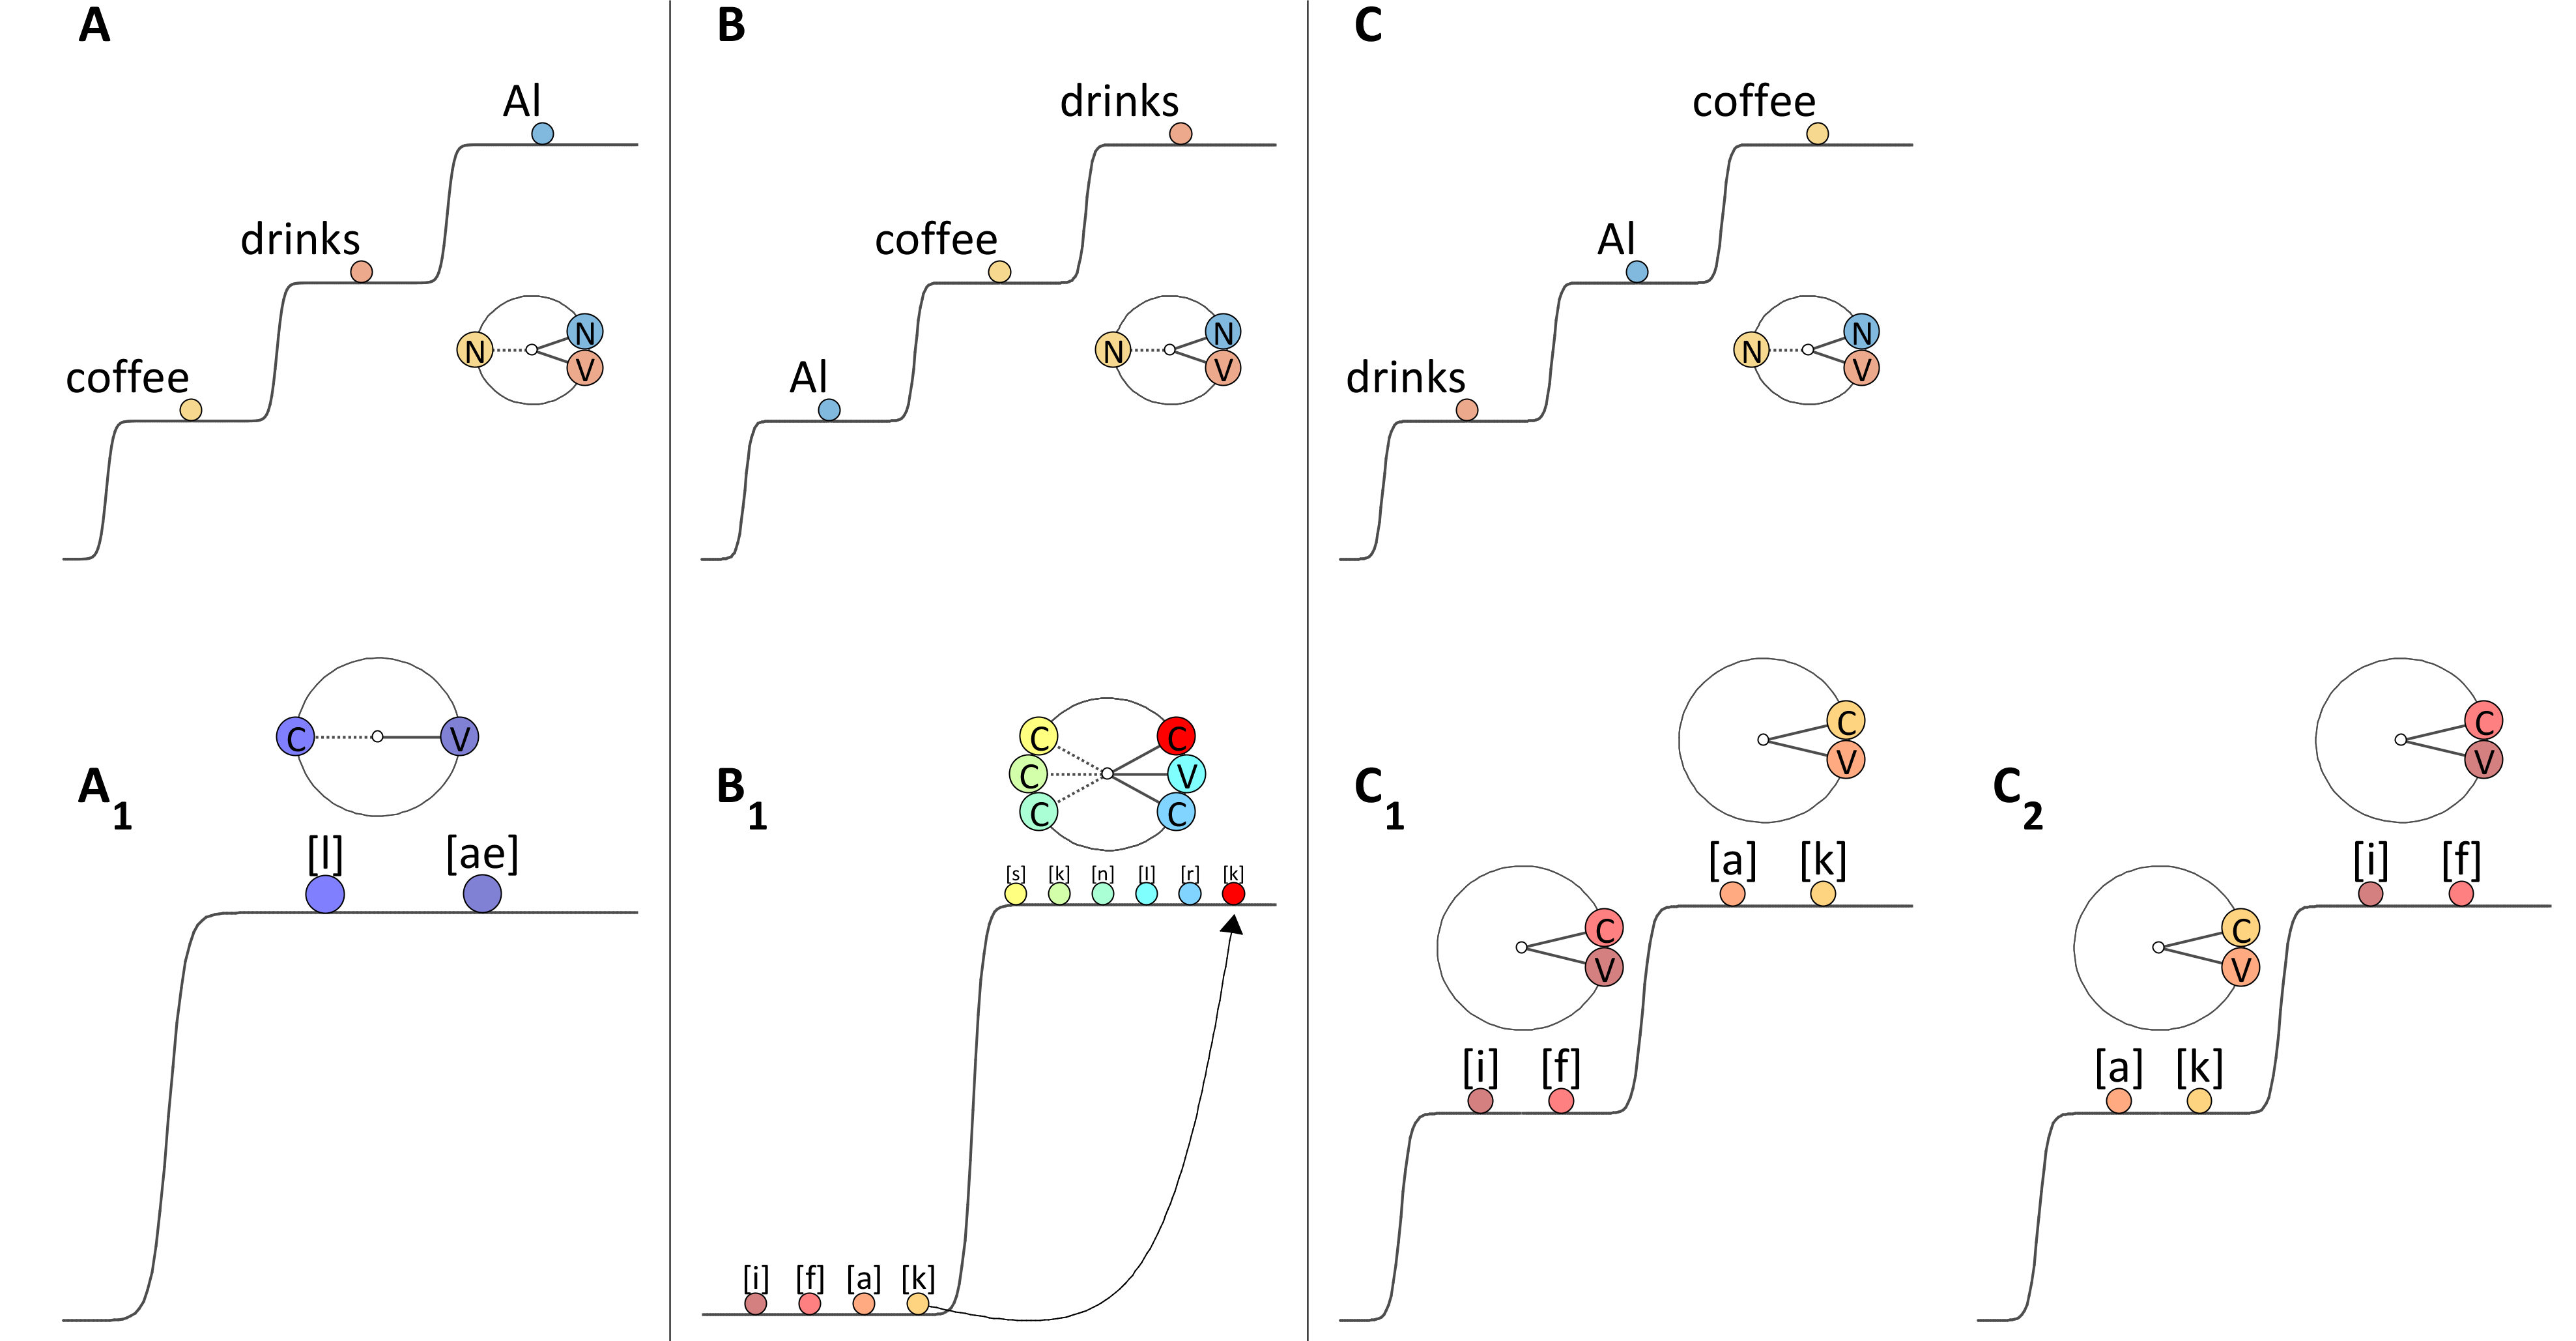
\includegraphics[width=\textwidth]{figures/Tilsen-img58.png}
\caption{\missingcaption}
\label{fig:4:8a}
\end{figure}
 

  However, even the above analysis of the disfluency mechanism as noncanonical competition is merely a guess. An alternative possibility is that some other cs-resonance we have not identified was active in epoch (B), and the g-domain of this unidentified system played a role. For example, a [cold] c-system might have been active throughout the utterance, as shown below. Despite being active, [cold] is never selected because it is unexcited. Nonetheless, systems in its g-domain are active and may, with help from other forces, become excited, which constitutes a deviation from the canonical trajectory.

  
\begin{figure}
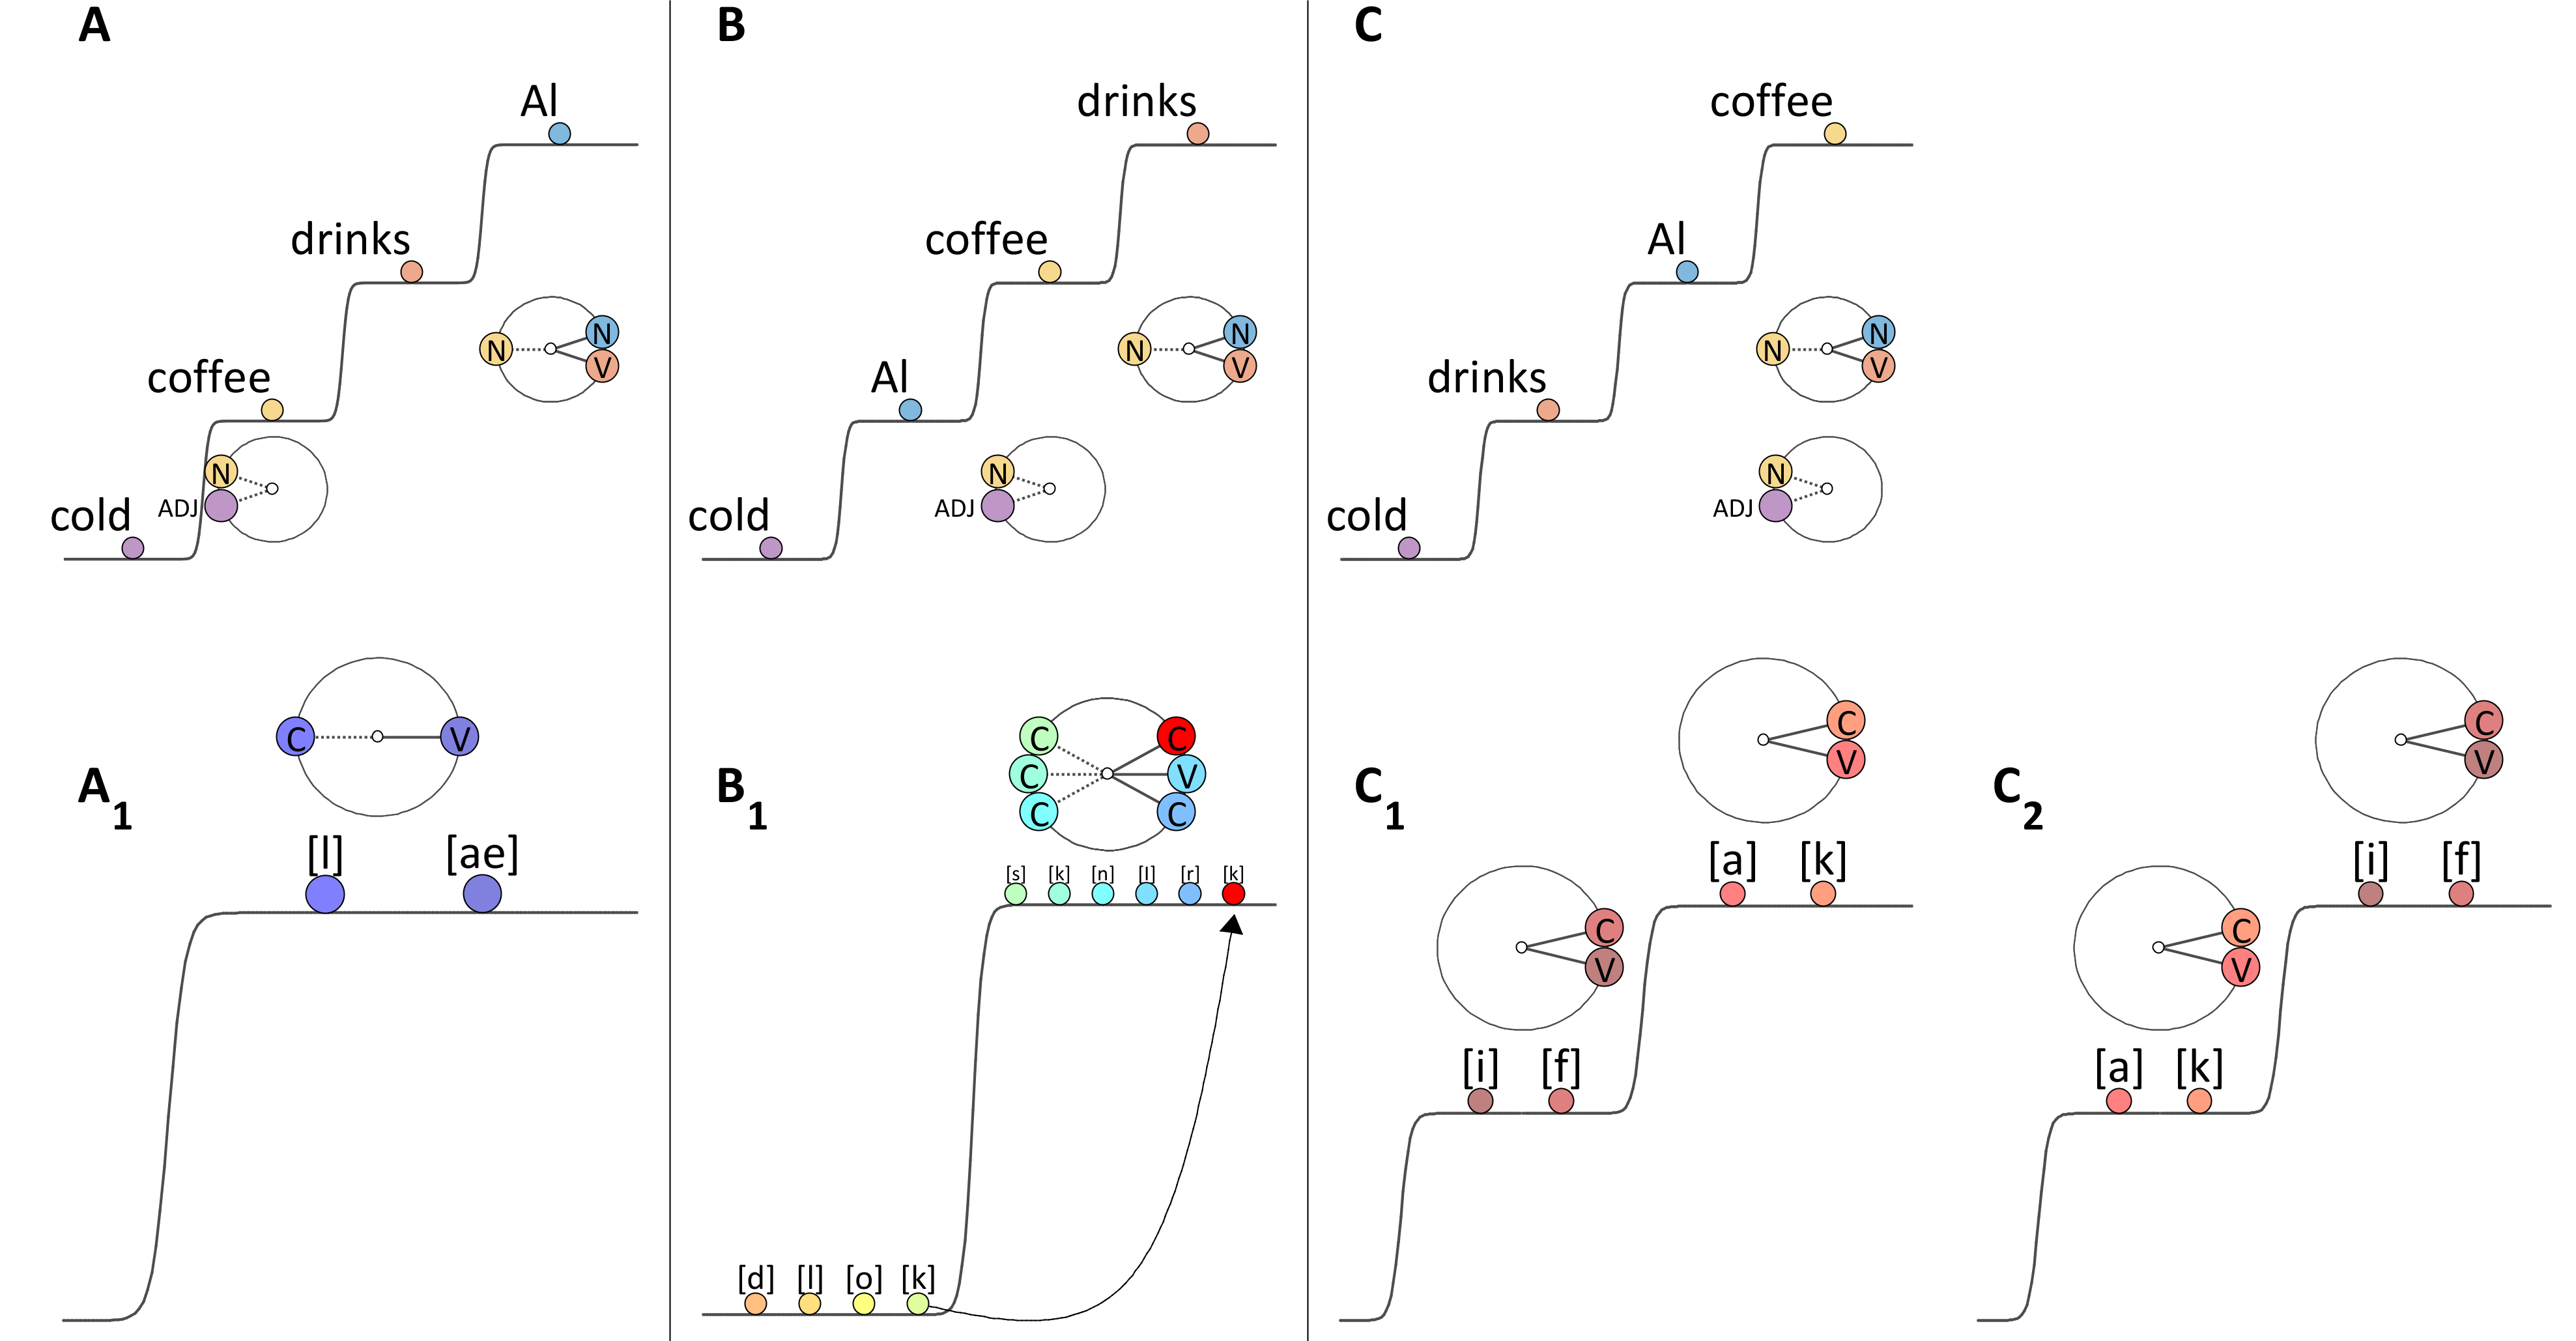
\includegraphics[width=\textwidth]{figures/Tilsen-img59.png}
\caption{\missingcaption}
\label{fig:4:8b}
\end{figure}
 

  If we allow for noncanonical reorganizations, there are even more possible analyses of disfluency mechanisms. For example, perhaps in epoch (e1) [craves]\{V\} was excited and [drinks]\{V\} unexcited, but surroundings forces caused a noncanonical reorganization to (e2), where [drinks]\{V\} is promoted to the selection level and [craves]\{V\} is grounded. Suppose the noncanonical reorganization interrupts execution of gm-systems. Such a trajectory might arise when competition between [craves] and [drinks] for \{V\} resonance continues after the initial organization and transition to a selective regime. 

  
\begin{figure}
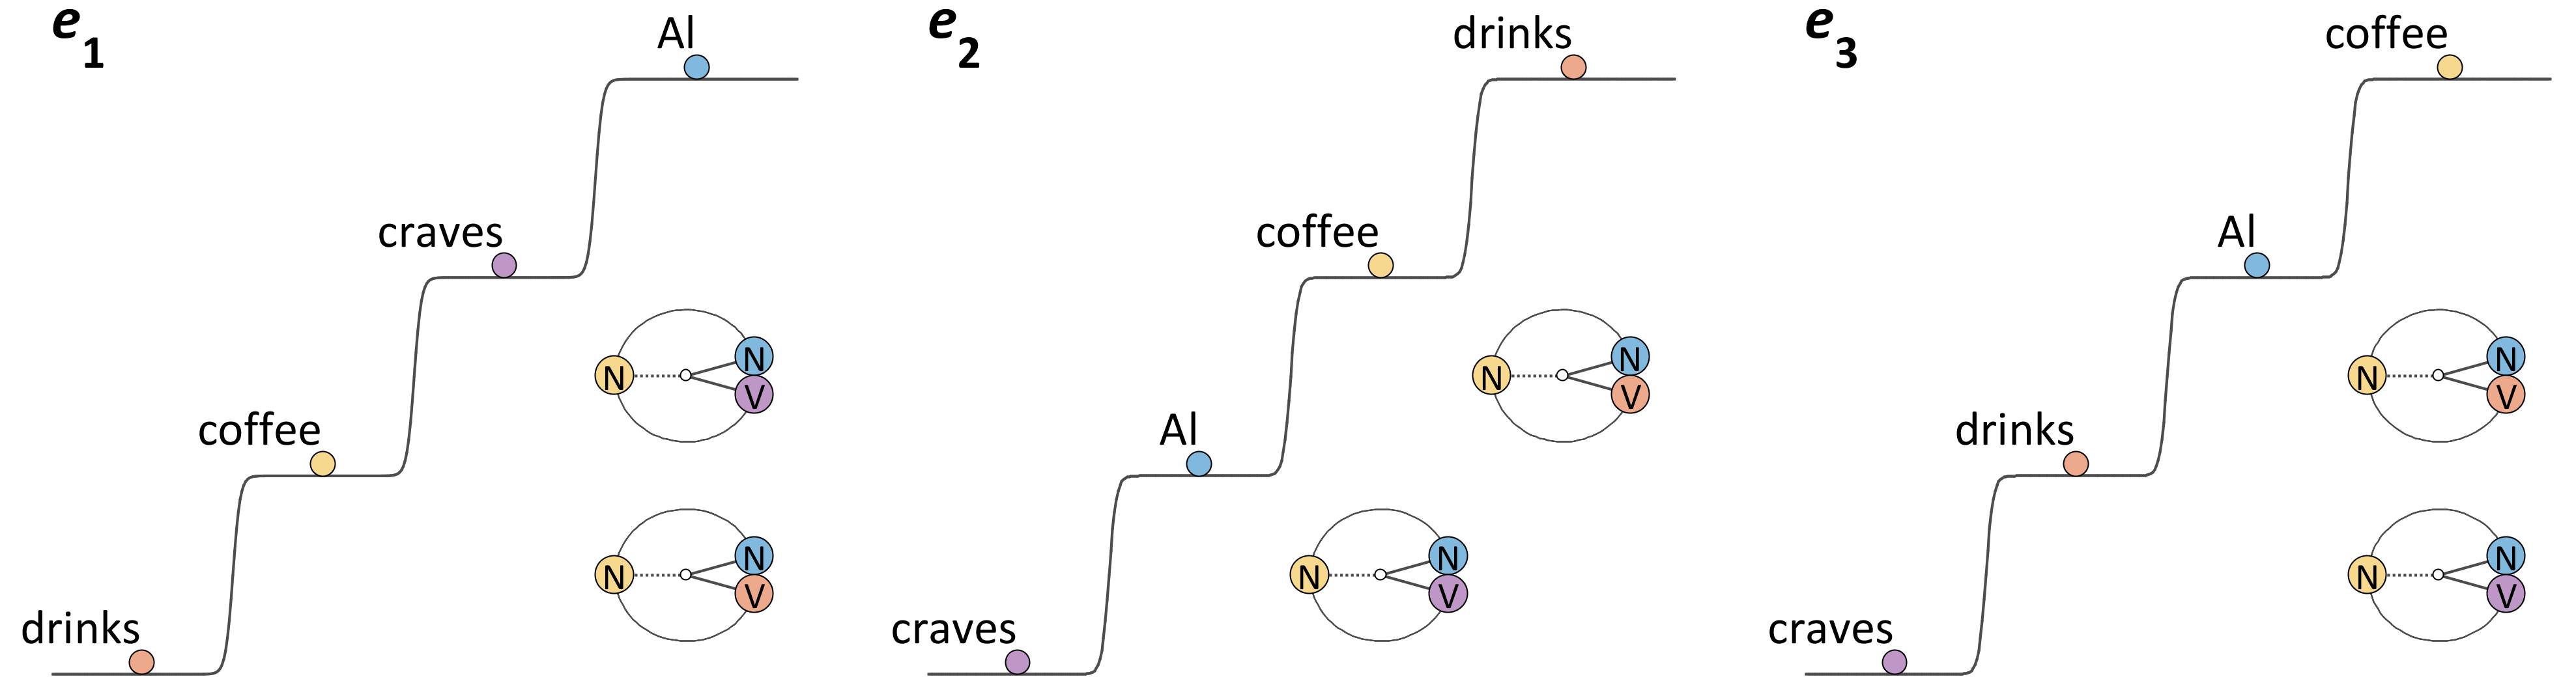
\includegraphics[width=\textwidth]{figures/Tilsen-img60.png}
\caption{\missingcaption}
\label{fig:4:10}
\end{figure}
 

  The above example illustrates why the notion of an intended canonical utterance/trajectory is problematic. What is the intended trajectory? Perhaps we might conduct the analysis with reference to two canonical trajectories, associated with \textit{Al craves coffee} and \textit{Al drinks coffee}. In some sense, both of these are the “intention” of the speaker. But in another sense, neither is an “intention”: the “intention” of the speaker was to change the trajectory from the one expected in (e1) to the one in (e2). Hence we might allow for the surroundings forces which cause the disfluency to be construed as intention. There are many disfluency manifestations which provide very little certainty regarding an intended trajectory. Thus rather than classifying observed disfluencies by guessing intentions, an alternative viable strategy for typologizing disfluencies is to classify ways in which perturbations of a canonical trajectory can map to manifestations.

  For a different example of disfluency, consider the utterance \textit{Al drinks…drinks coffee}, where the speaker hesitates after the first production of \textit{drinks} and repeats \textit{drinks}. Perhaps a c-system such as [tea] competes with [coffee] for cs-resonance with \{-N\}, and perhaps both [tea] and [coffee] are excited in the initial e-organization (e1). Because of this circumstance, reorganization from (e2) to (e3) fails to promote either [tea]\{-N\} or [coffee]\{-N\} to selection level. Instead, there is a period of time in which no cs-system is selected (a hesitation), while the [coffee]-[tea] competition is resolved by grounding [tea]\{-N\}. Eventually, a noncanonical reorganization to (e4) occurs, which promotes [drinks]\{V\} to selection level a second time. 

  
\begin{figure}
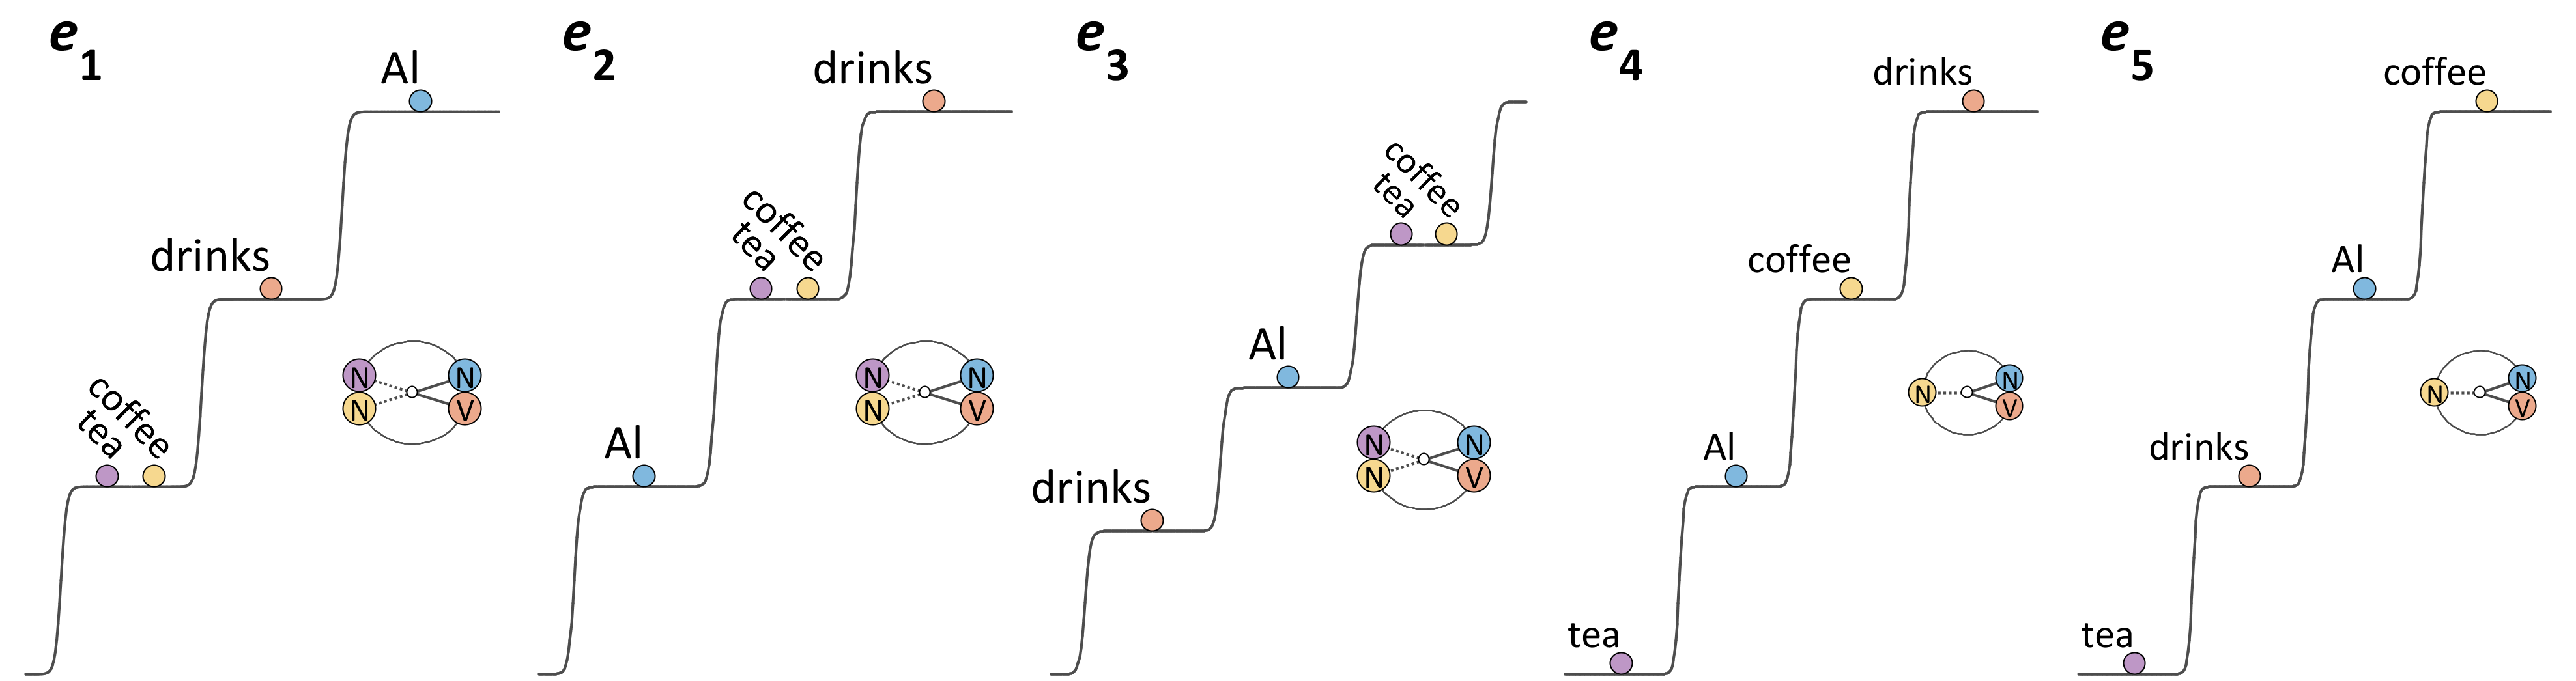
\includegraphics[width=\textwidth]{figures/Tilsen-img61.png}
\caption{\missingcaption}
\label{fig:4:11}
\end{figure}
 

  By considering other noncanonical reorganizations, we can generate alternative manifestations. If the post-hesitation reorganization promotes both [Al]\{+N\} and [drinks]\{V\}, the utterance would be \textit{Al drinks…Al drinks coffee}. If the reorganization promotes no cs-systems, the utterance would be \textit{Al drinks…coffee}. If detection of the promotion failure closes s-gates temporarily, perhaps an [uh] gm-system is selected during the hesitation, and the utterance is \textit{Al drinks…uh…coffee}.

  Another example of disfluency involves a mechanism in which external feedback does not match a conceptual state—a self-monitoring disfluency. Consider the utterance \textit{Al drinks tea…coffee.} We might imagine that the utterance is produced in accordance with an canonical trajectory for \textit{Al drinks tea} (e1-e3), but for whatever reason, the speaker transitions between (e3) and (e4) to attending to an {\textbar}Al drinks coffee{\textbar} φ configuration instead of {\textbar}Al drinks tea{\textbar}. As a consequence, external feedback of [tea] is not consistent with the φ configuration which involves [coffee]; this leads to a reorganization which promotes [coffee] to selection level.

  
\begin{figure}
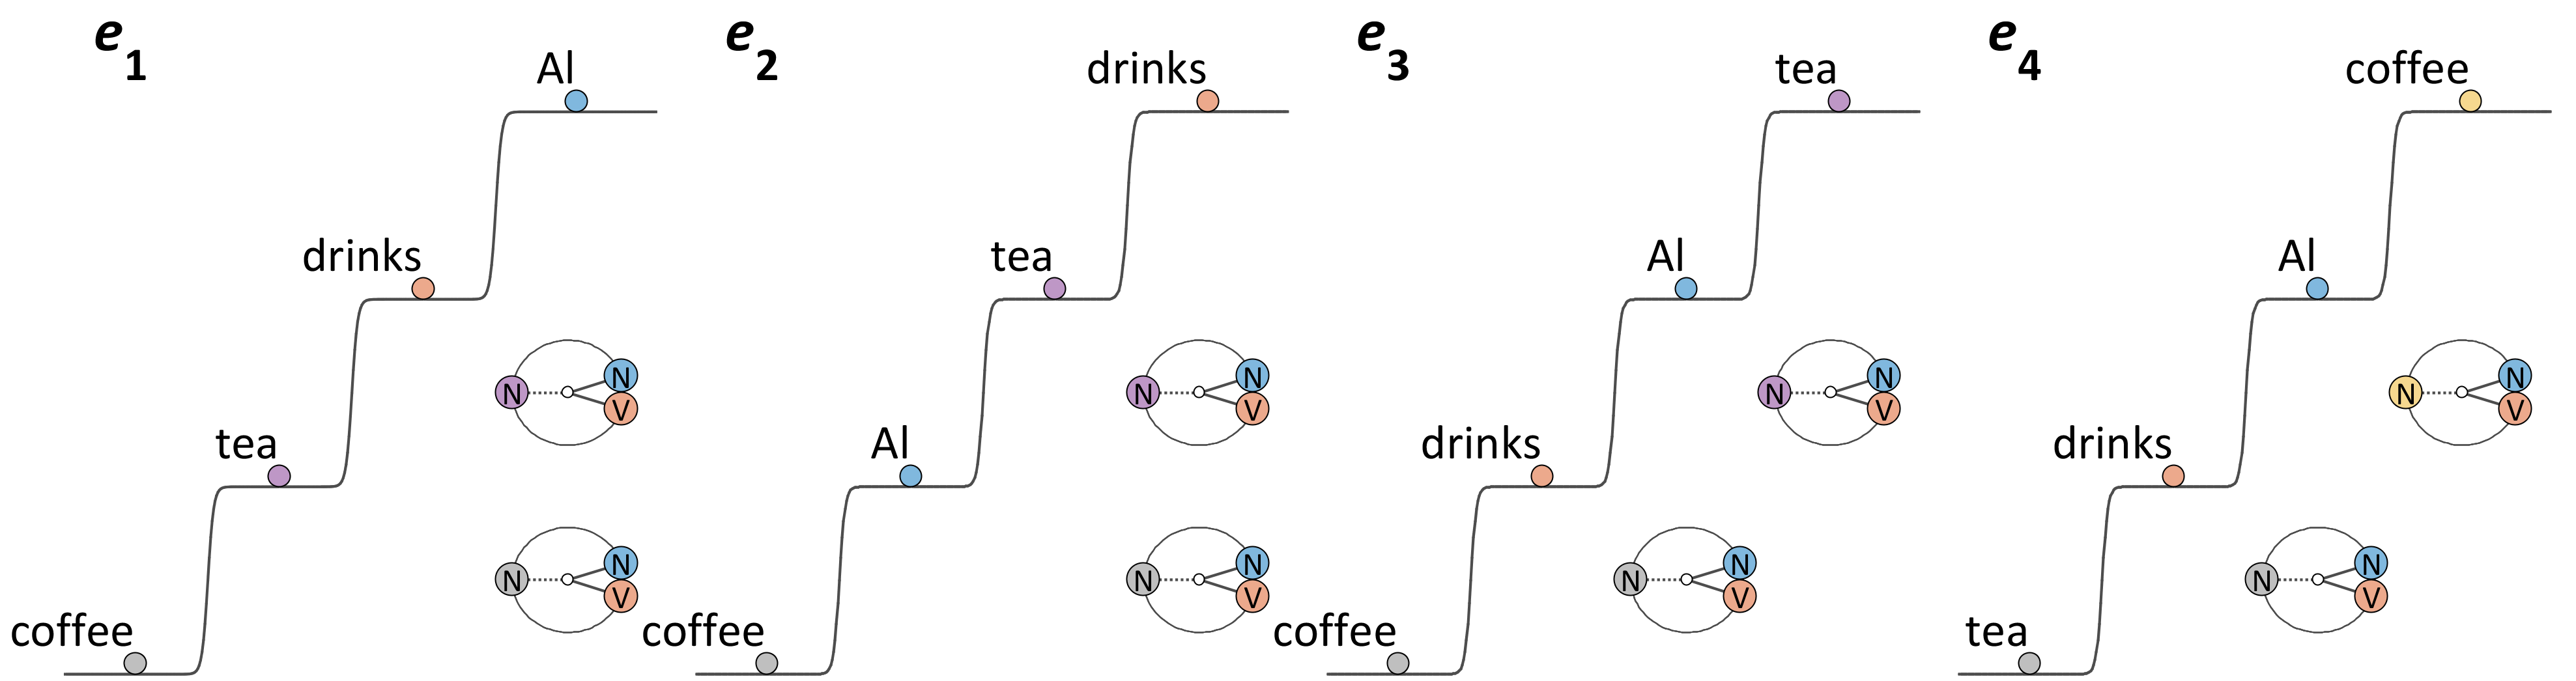
\includegraphics[width=\textwidth]{figures/Tilsen-img62.png}
\caption{\missingcaption}
\label{fig:4:12}
\end{figure}
 

  By systematically analyzing ways in which production trajectories can deviate from canonical ones, and comparing these to observed manifestations, it should be possible to gain greater insight into constraints on the reorganization operator, Ê. This sort of approach also usefully structures our analysis of observed disfluencies, by compelling us to be more aware of the our assumptions regarding speaker intentions.

\subsection{Accentual and metrical patterns}

One pervasive form of cs-gm interaction involves accentual patterns such as primary stress or lexical pitch accent. In some languages, we hypothesize a class of \textit{accentual} g-systems which resonate with an accentual m-system, \{A\}. Accentual g-systems often involve tones (or pitch accents), such as [H*]. Consider the accentual pattern on the phrase \textit{Mr}. \textit{Mississippi}, as shown below. Following our previous analyses, we might conceptualize the gm-system [H*]\{A\} as the gm-domain of an accentual [\textsc{accent}]\{A\} cs-system. In other words, we could posit a class of accentual c-systems [\textsc{accent}] and a corresponding class of s-systems, \{A\}. However, there are some problems with this analysis. In many cases the participation of the [\textsc{accent}]\{A\} system in a relational meaning experience is hard to characterize. Moreover, we have no reason to suspect that [\textsc{accent}]\{A\} needs be reorganized like other cs-systems, because all selective epochs can include selection of [\textsc{accent}]\{A\}, and many stress/pitch accent languages have a default gm-domain for [\textsc{accent}].

  
\begin{figure}
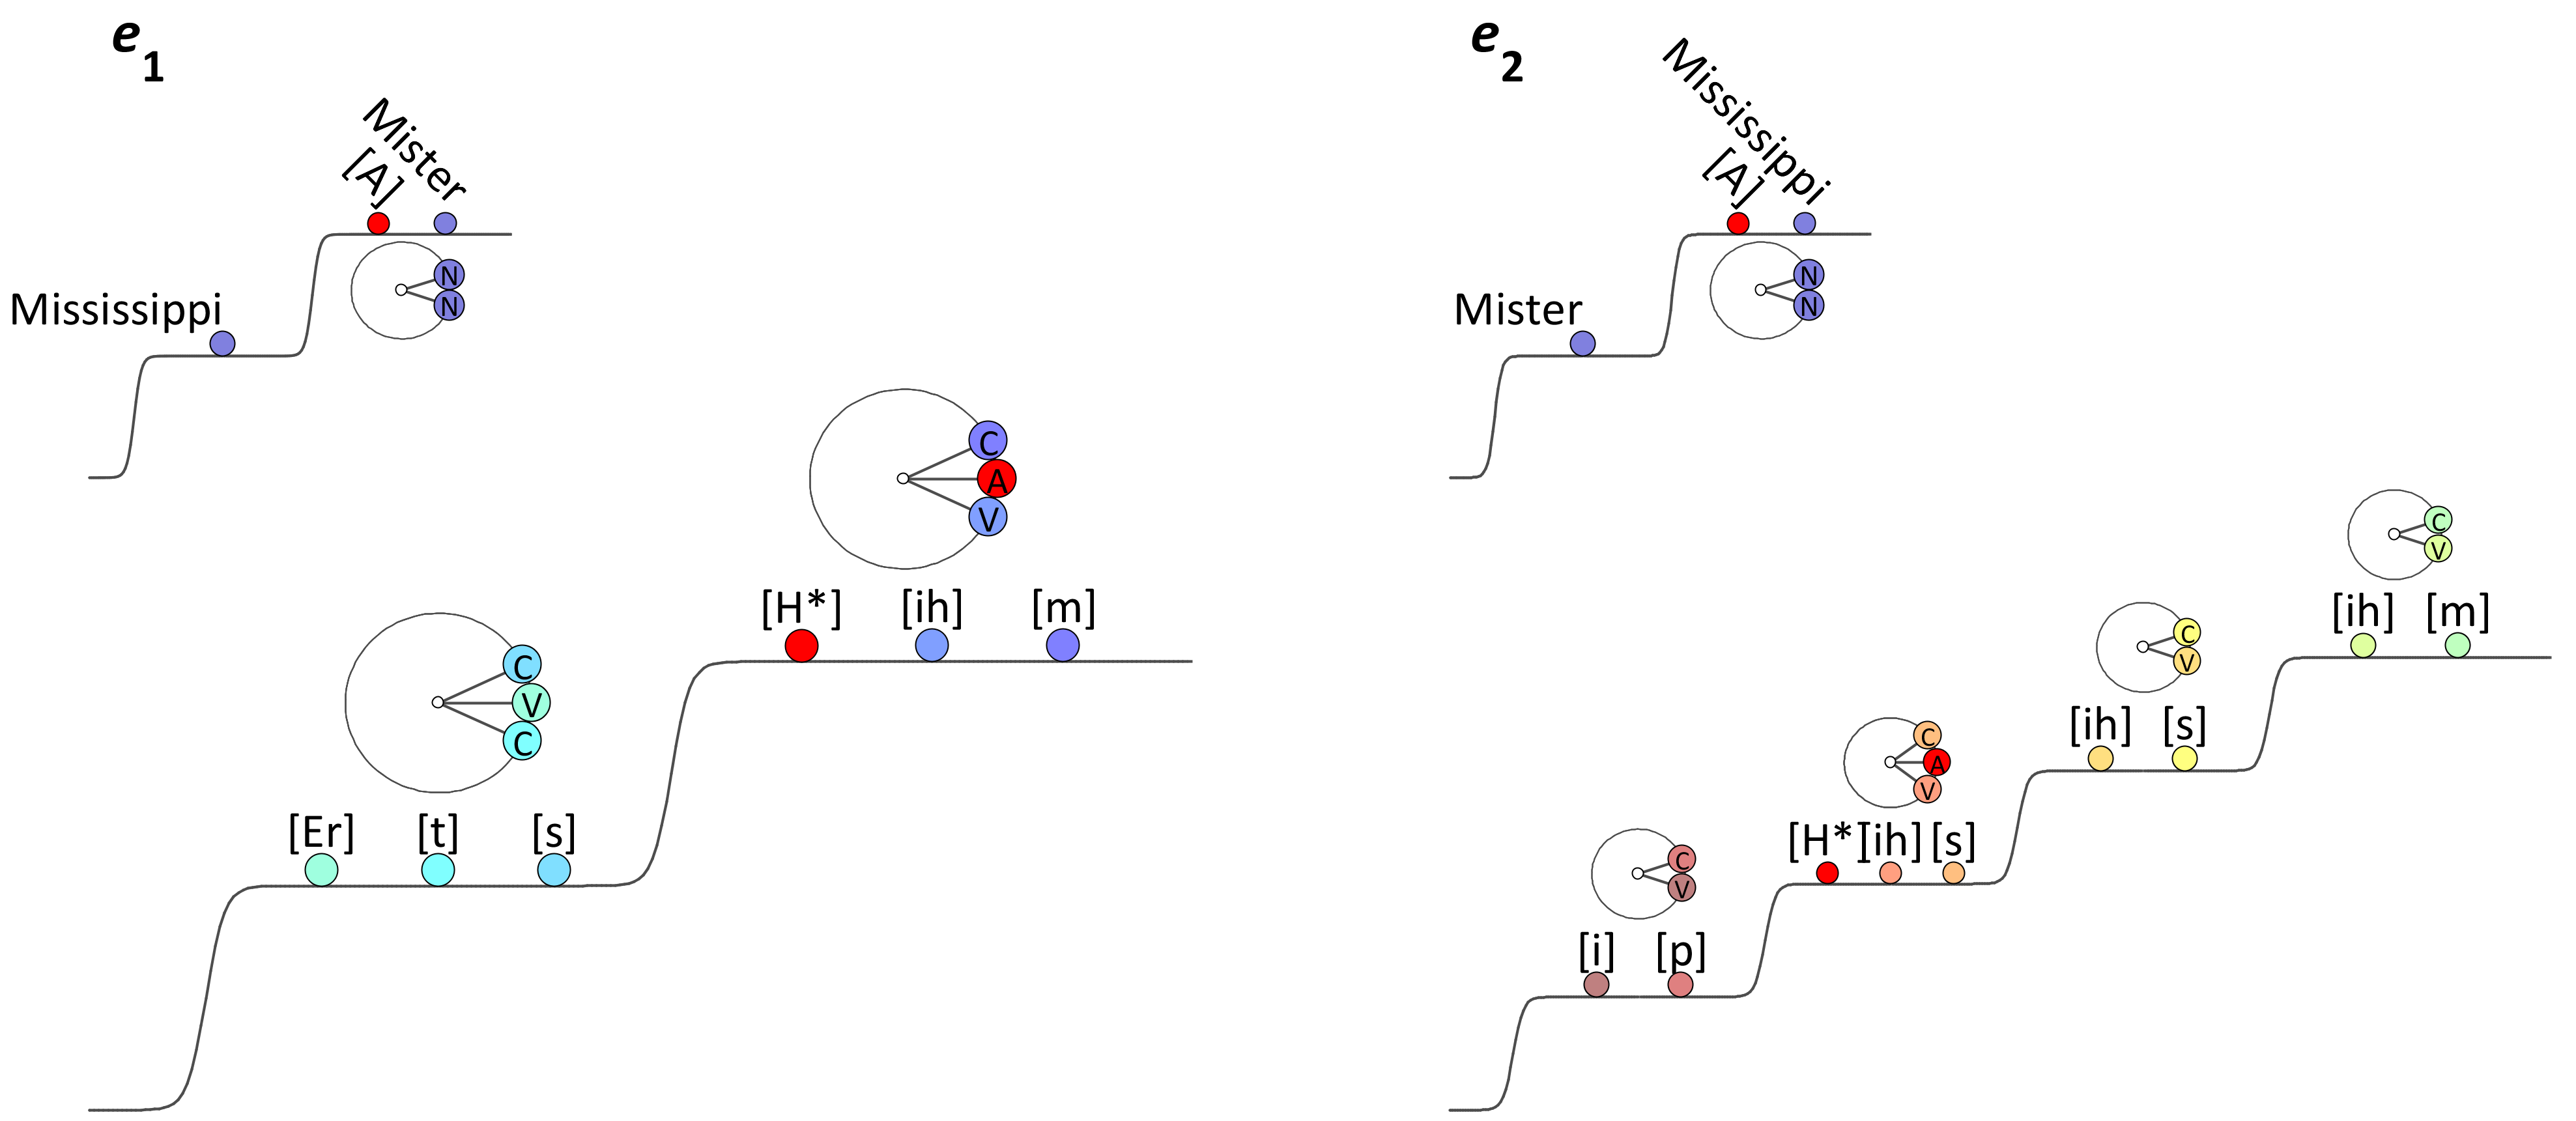
\includegraphics[width=\textwidth]{figures/Tilsen-img63.png}
\caption{\missingcaption}
\label{fig:4:13}
\end{figure}
 

  Indeed, the observation that an accentual system can be selected once in each epoch, regardless of which other cs-systems are selected, suggests that we view the accentuation system differently. The alternative we pursue is to posit a special accentual s-system \{\^{}\}. The s-system \{\^{}\} does not differentiate like other s-systems; instead \{\^{}\} is selected and re-selected in each selective epoch and potentially excites the gm-domain of an accentual c-system, i.e. [\textsc{accent}], without necessarily φ-coupling to that c-system. In the case of intonational accents, we imagine that different varieties of [\textsc{accent}] c-systems (e.g. [\textsc{contrast}], [\textsc{focus}], [\textsc{surprise}]) may couple to lexical s-systems, and that \{\^{}\} excites the gm-domains of those [\textsc{accent}] c-systems. In the absence of a more specific c-system being excited, a default gm-domain may be excited by \{\^{}\}. This circumstance accounts for the typological pattern of \textit{stress}, where each set of co-selected cs-systems is produced with one primary accent. This could be a default gm-system or a more pragmatically meaningful one that is the domain of [\textsc{contrast}], [\textsc{focus}], etc. For patterns called \textit{pitch accent}, the gm-domain of \{\^{}\} can be determined by the co-selected cs-system.

  The metrical organization of accentual gm-systems relates to how the m-system \{A\} is organized in a multi-level gm-domain. For example, the gm-configuration of \textit{Mississippi} has four e-levels, and \{A\} initially occupies the third e-level. In some languages the organization of \{A\} is determined entirely by the number of e-levels in the gm-domain (fixed stress). In other languages the organization of \{A\} can be influenced by the identity of the selected cs-system (free stress). In both cases, the compositions of the gm-systems may influence \{A\} organization (quantity sensitivity). 

  To account for secondary stress in the gm-domain of co-selected cs-systems, we hypothesize that gm-configuration re-organization can be driven by rhythmic m-system selection. As shown below, co-selected \{+C\}\{V\} m-systems are +φ-coupled. Constructive interference between m-systems occupying different e-levels is maximized when oscillation phases align. We can associate the maximized constructive interference pattern with \textit{periodic e-reorganization} and an reorganization frequency, \textit{f}\textsuperscript{0}. Periodic reorganization occurs when there is a periodicity which strongly influences the timing of promotion and demotion (i.e. the canonical reorganization regime). Importantly, periodic reorganization is not a general mechanism of conversational speech. Instead, it is a regime associated with specialized contexts, e.g. poetic meter/rhythmic speech, entrainment to external stimuli, and analytical reflection on metrical patterns—i.e. metrical intuition formation. Periodic reorganization may also be a developmental mechanism for stabilizing e-reorganization processes, as in babbling. In disfluency and some disordered speech, it may emerge as a stabilizing mechanism.

  
\begin{figure}
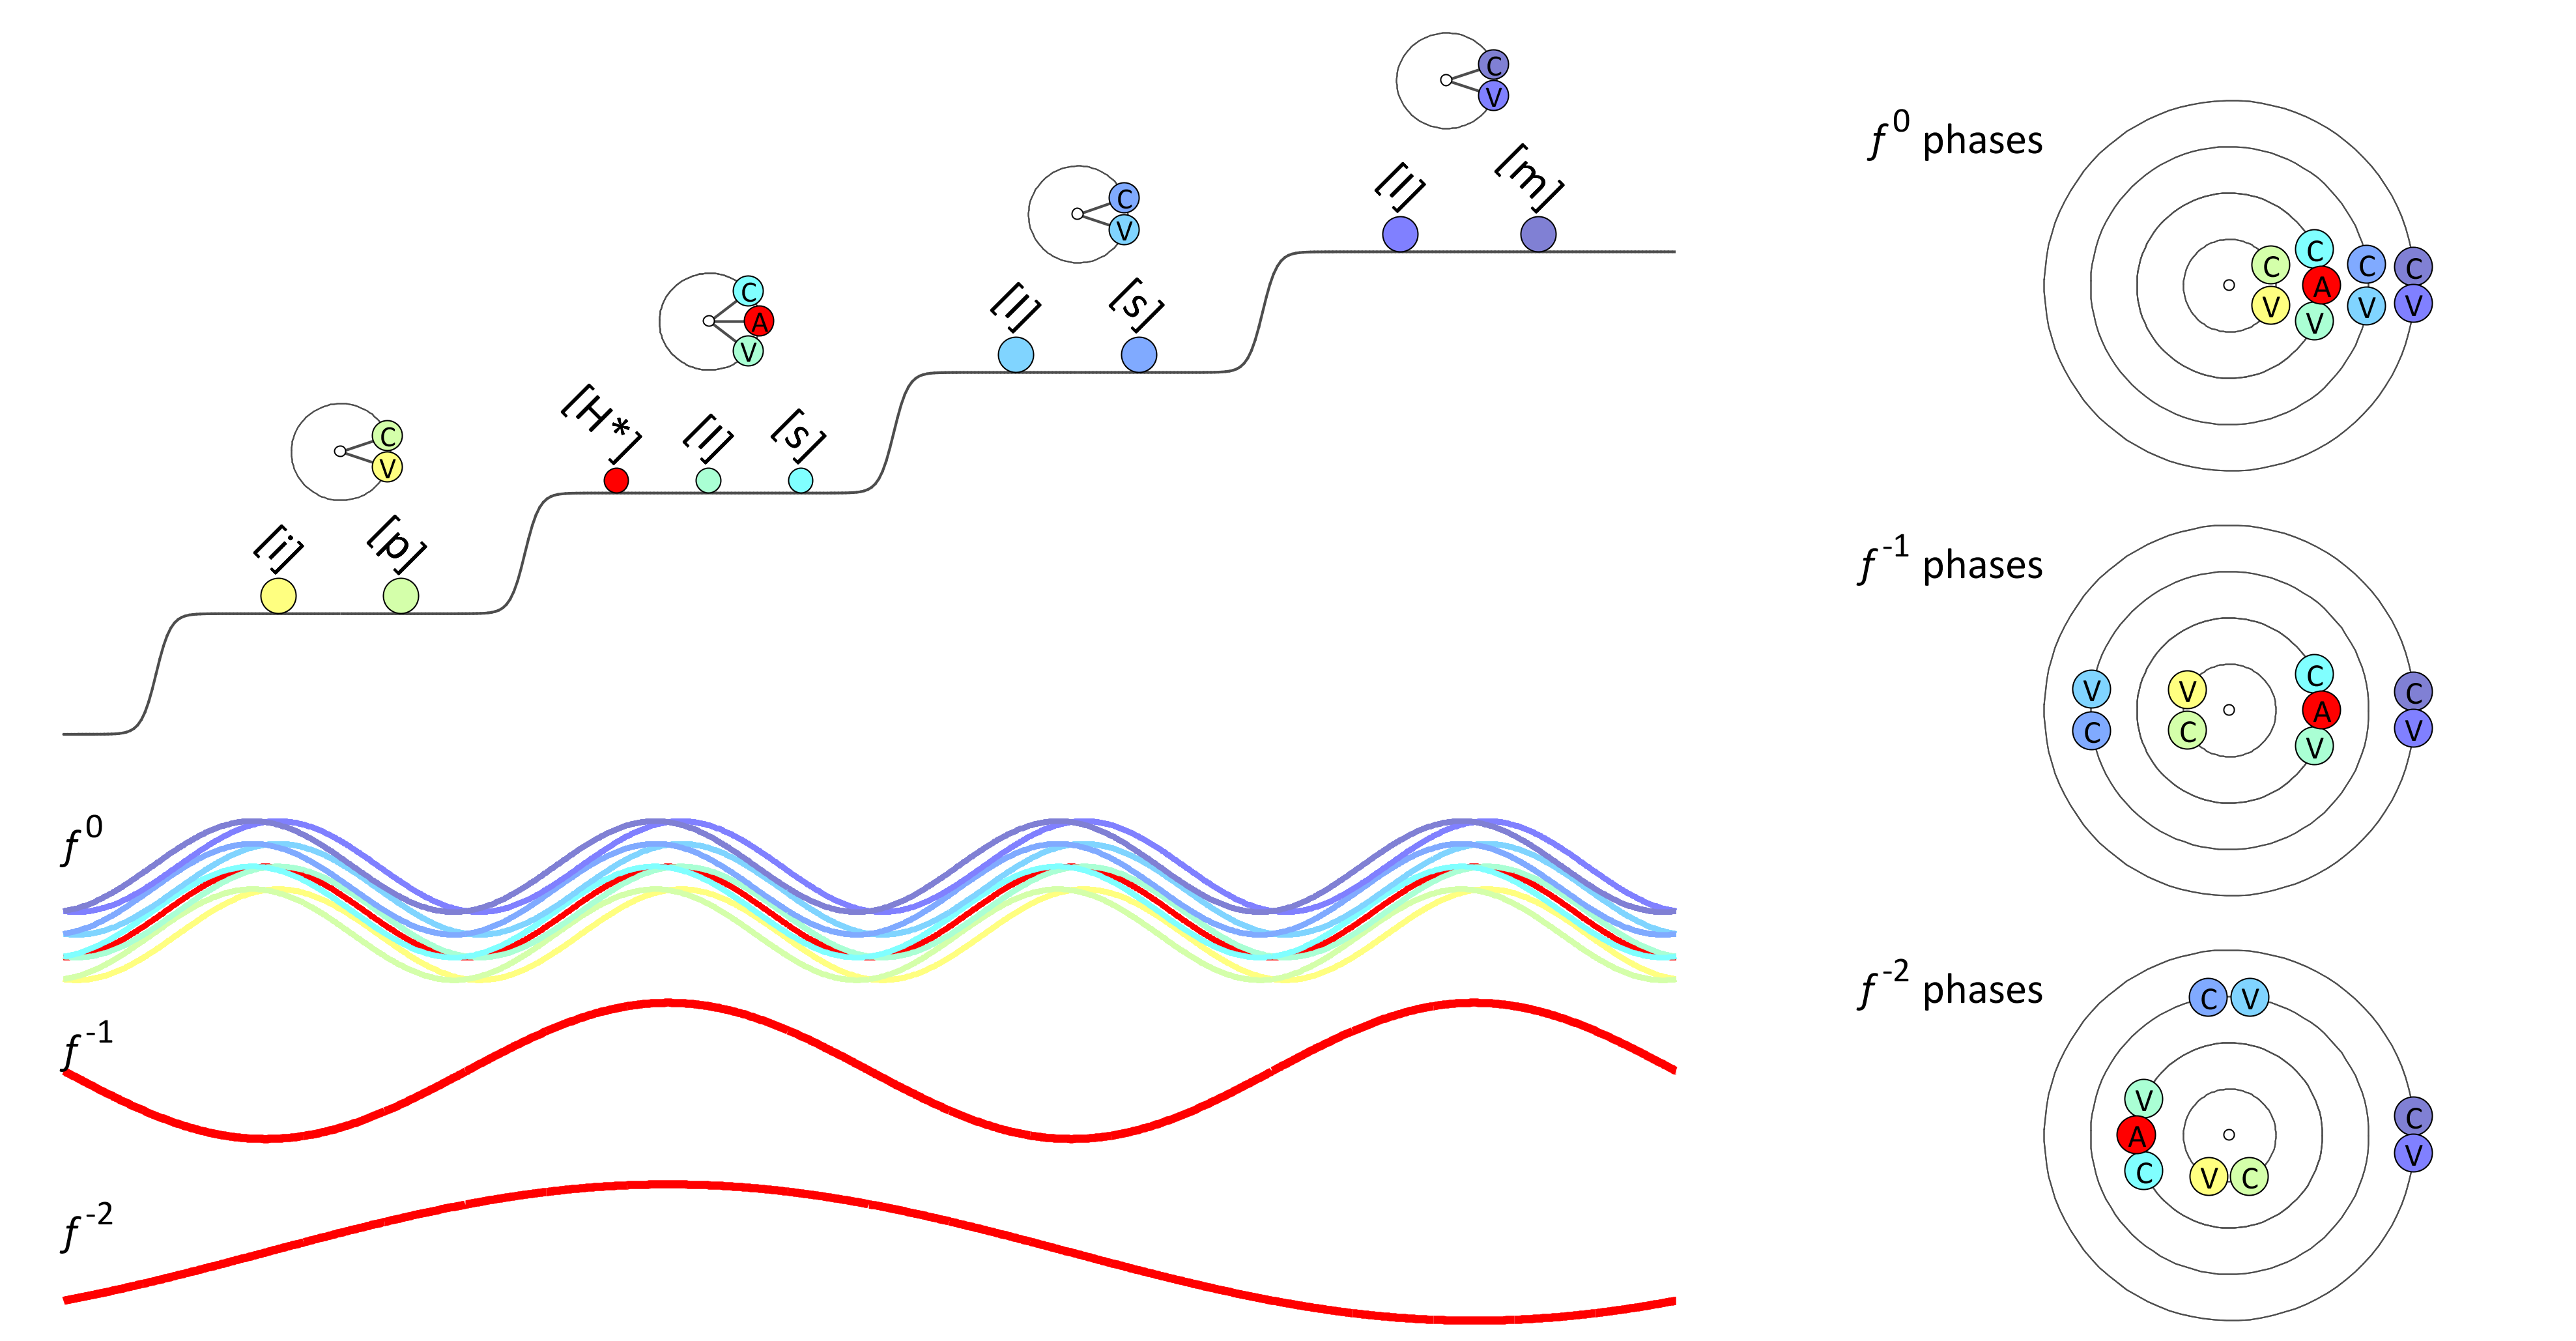
\includegraphics[width=\textwidth]{figures/Tilsen-img64.png}
\caption{\missingcaption}
\label{fig:4:14}
\end{figure}
 

  To reconceptualize higher-level prosodic organization, we hypothesize that the maximized constructive interference pattern facilitates the emergence of subharmonic oscillations at frequencies \textit{f}\textsuperscript{{}-1}, \textit{f}\textsuperscript{{}-2},… \textit{f}\textsuperscript{{}-n} and that cs-systems can φ-couple to these subharmonics via coupling of generalized relative phase, i.e. φ\textsubscript{ij} = 2π(\textit{f}\textsubscript{j}θ\textsubscript{i} - \textit{f}\textsubscript{j}θ\textsubscript{i}). If subharmonic oscillations are influential during a developmental stage in which rhythmic e-reorganization is a heuristic/bootstrapping mechanism, speakers might learn to +φ-couple \{A\} m-systems with the lowest subharmonic oscillation.

\section{Morphosyntax and morphophonology}
\rohead{\headmark}
\subsection{Grammatical vs. lexical systems}

Up to this point, our analyses have focused on \textit{lexical} cs-systems. For example, we have ignored the fact that the word \textit{drinks} in \textit{Al drinks coffee} is associated with grammatical person and number. We can elaborate our analyses by including state space dimensions for \textit{grammatical} cs-systems, i.e. systems which evoke so-called \textit{functional} or \textit{grammatical} meaning, e.g. tense, aspect, mood, voice, person, number, gender, case, definiteness, etc. A variety of differences between grammatical and lexical systems are enumerated below. However, one should infer no \textit{essential} distinction between these types of systems; “grammatical system” and “lexical system” are analytical categories, which have more or less prototypical members and heterogeneous category structure. On historical scales, more prototypically grammatical systems tend to evolve from more prototypically lexical ones, and hence we expect intermediate varieties and cases in which different types of cs-systems are associated with the same or similar gm-domains. 
\begin{enumerate}

\item Grammatical c-systems resonate with grammatical s-systems through +φ-coupling, just like lexical c-systems resonate with lexical s-systems such as \{N\}, \{V\}, \{Adj\}, \{Adv\}. We construct various types of grammatical s-systems for various types of grammatical c-systems. Hence to understand how a concept of 3\textsuperscript{rd} person is evoked in a relational meaning experience, we construct a [3\textsuperscript{rd}] c-system, an s-system \{\textsc{person}\}, and a cs-resonance [3\textsuperscript{rd}]\{\textsc{person}\}. 

\item Like lexical cs-resonances, grammatical cs-resonances are canonically one-to-one, i.e. a grammatical c-system will strongly resonate with only one grammatical s-system in a local epoch, and vice versa. The reason for this is interference: before φ-stabilization, c- and s- systems will generally have different angular velocities $\theta ′$ and phases θ. This makes configurations with many-to-one resonances unstable (we examine interference in more detail, later in this chapter).

\item Lexical and grammatical c-system networks exhibit a variety of differences. Grammatical c-systems which resonate with the same class of s-system exert relatively strong inhibitory forces on each other, while lexical c-systems exert relatively weak inhibitory forces. To elaborate the intuition behind this, lets assume that for each s-system we can identify a \textit{c-domain} as the set of all c-systems which may resonate with the s-system. Hence the c-domain of \{\textsc{person}\} is [\textsc{1}\textsc{\textsuperscript{st}}], [\textsc{2}\textsc{\textsuperscript{nd}}], [\textsc{3}\textsc{\textsuperscript{rd}}]. The c-domain of a lexical s-system such as \{V\} has many more c-systems in its c-domain than \{\textsc{person}\} does. Imagine these networks of interactions between c-systems as below. Our intuition is that grammatical c-domain networks are fully connected and have relatively strong, inhibitory e-coupling forces between all systems, whereas lexical c-domain networks are sparsely connected with relatively weak e-coupling, which may be of either negative (-e) or positive (+e) valence.

  
\begin{figure}
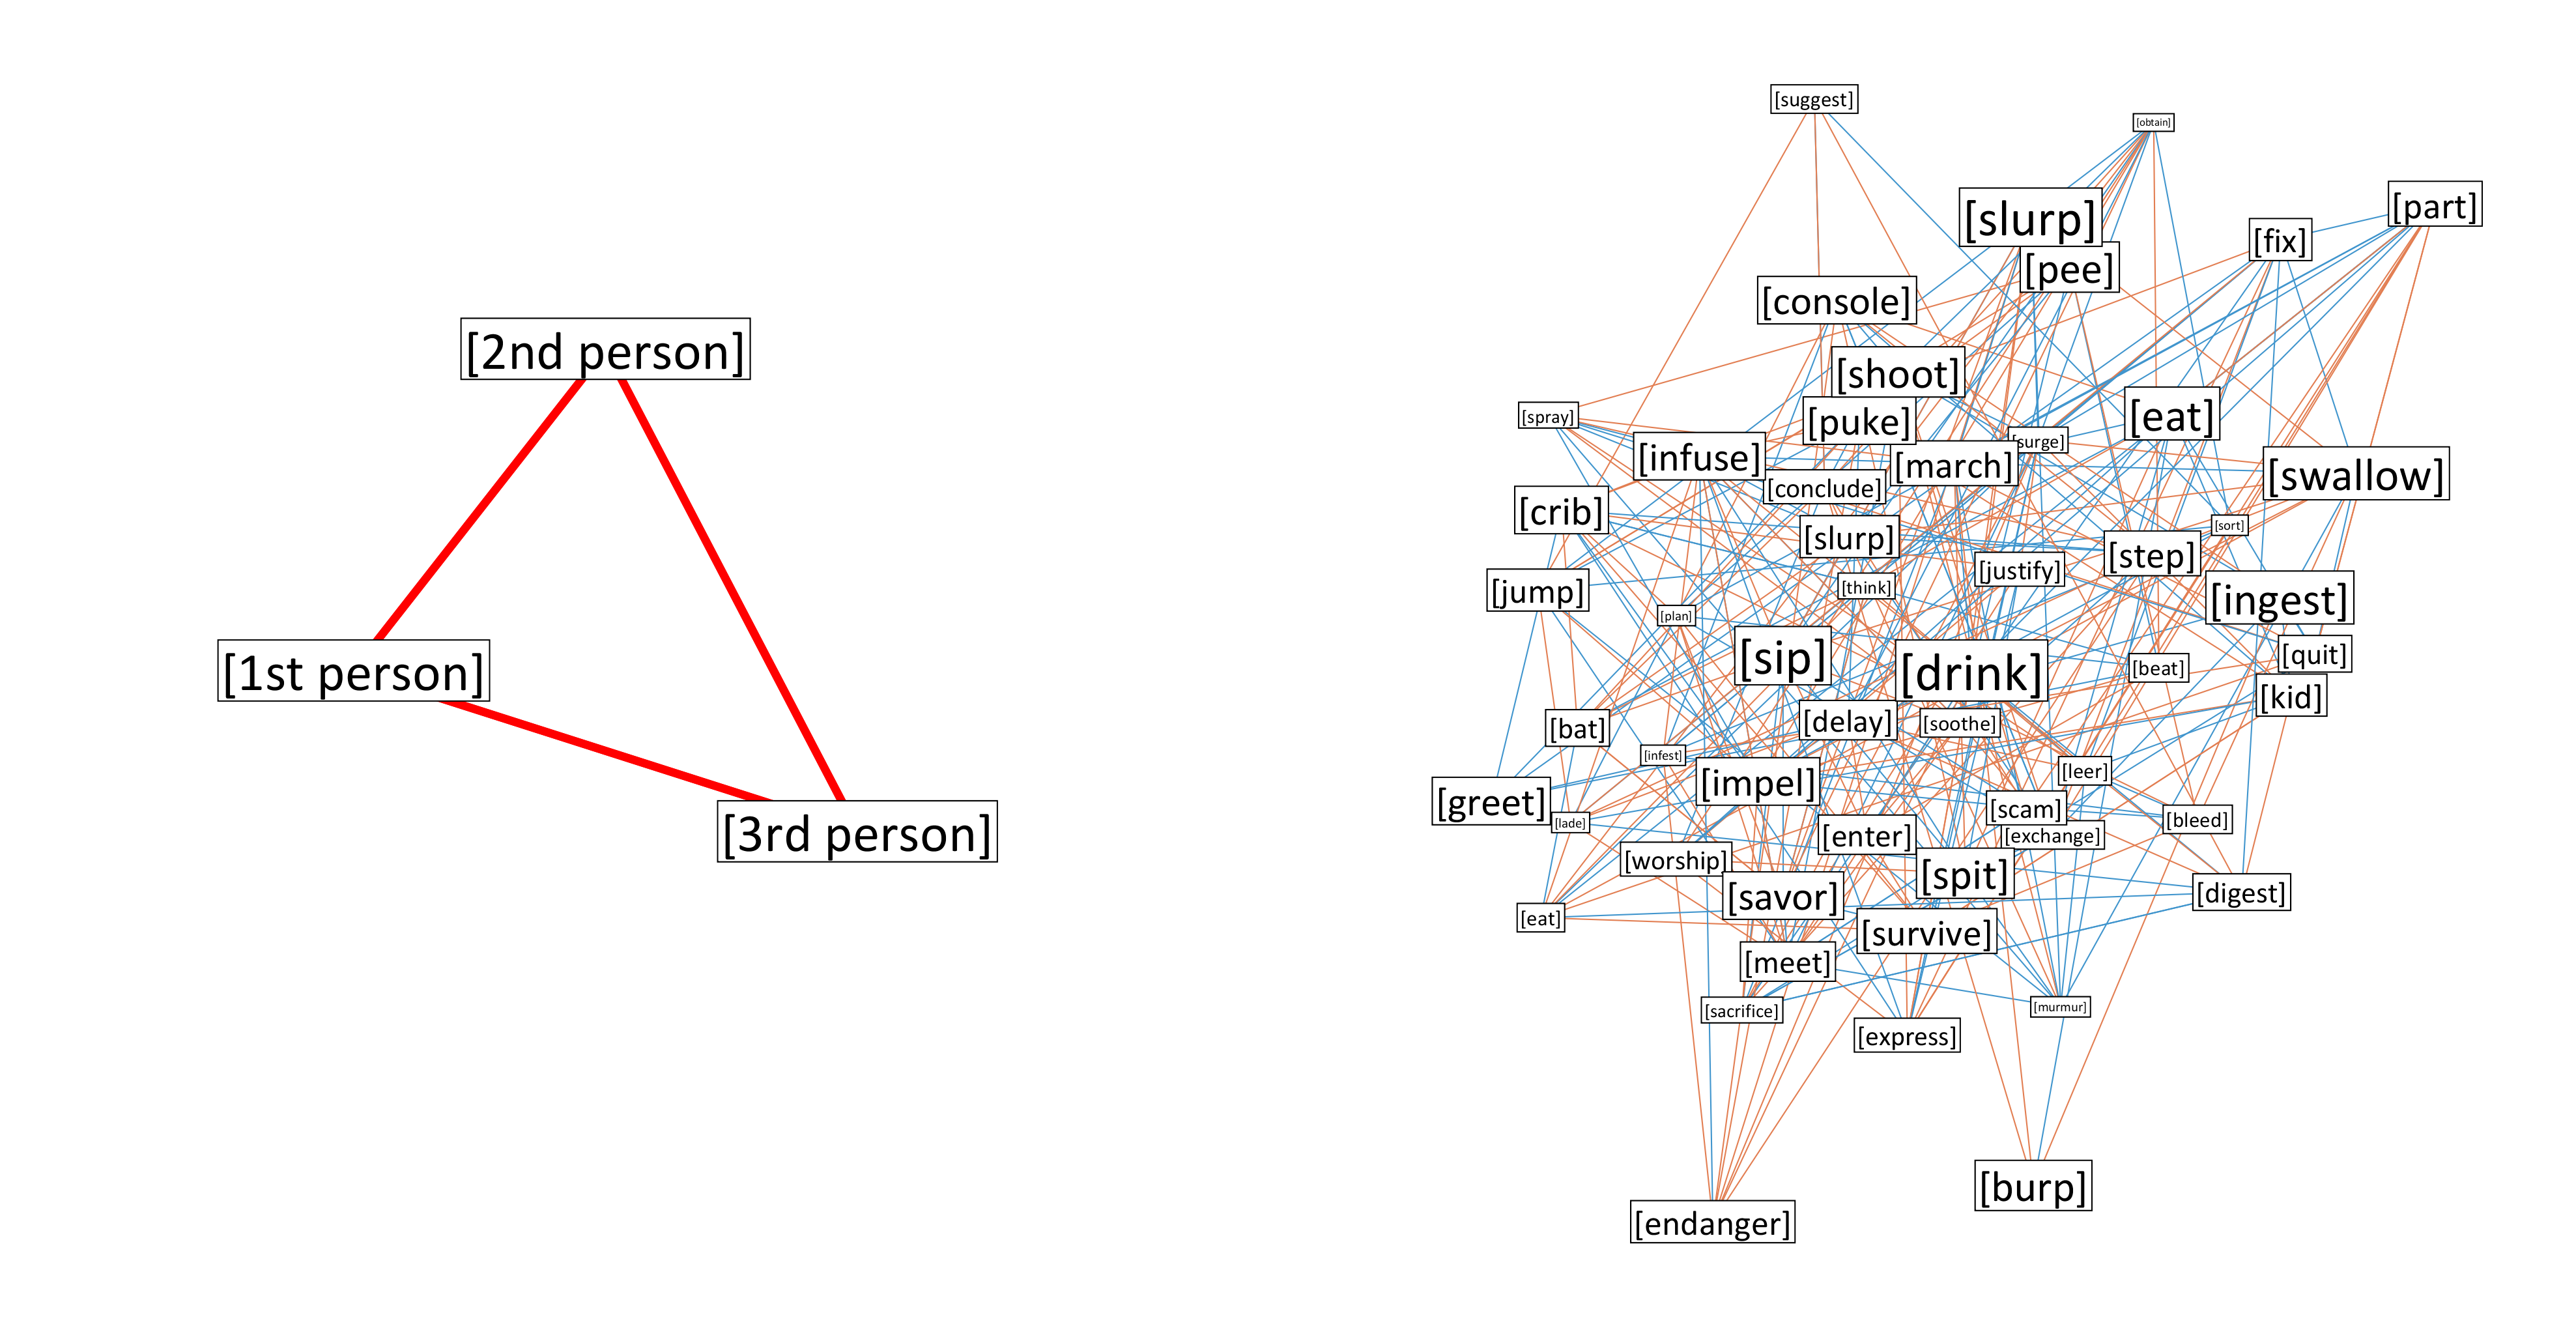
\includegraphics[width=\textwidth]{figures/Tilsen-img65.png}
\caption{\missingcaption}
\label{fig:4:15}
\end{figure}
 

\item On supra-utterance scales, there are statistical differences in how often grammatical and lexical cs-systems are excited: typical grammatical cs-systems are excited more frequently than lexical ones. The greater occurrence frequency correlates with differences in c-domain network structure, and this should be derivable from a microscopic model. The difference between +e and -e coupling derives from the relative proportion of postsynaptic targets of projections between populations: projections from excitatory neurons in one population to excitatory neurons in the other population promote +e coupling; projections to inhibitory interneurons promote -e coupling. The numbers of such projections between any two populations, along with their synaptic weights, is influenced on supra-utterances scales by learning mechanisms such as spike-timing dependent plasticity. The macroscale consequence is that in grammatical c-domains, because of the greater occurrence frequency of grammatical cs-resonances, c-systems evolve to exert and experience stronger e-coupling forces on other grammatical c-systems, compared to lexical c-domain networks. Hence our microscale conceptualization predicts a correlation between occurrence frequency and within-domain connectivity/coupling strengths.

\item  In order for a grammatical cs-system to participate in a relational meaning experience, the grammatical s-system must φ-couple with a lexical s-system. The valence of this coupling is always +φ. For \textit{Al drinks the coffee} shown below, this entails that \{\textsc{person}\} and \{\textsc{number}\} are +φ coupled to \{V\}, and \{D\} is +φ coupled to \{-N\}. Consequently [\textsc{3}\textsc{\textsuperscript{rd}}] and [\textsc{sg}.] have a +φ relation to [drink], and [\textsc{definite}] has +φ relation to \{-N\}.

\item Grammatical s-systems are often organized in the same e-level as the lexical s-system they are φ-coupled to. An example is shown below, where [3\textsuperscript{rd}]\{\textsc{person}\} and [\textsc{sg.}]\{\textsc{number}\} are on the same level as [drink]\{V\}, and [\textsc{def}.]\{D\} is on the same level as [coffee]\{-N\}. This entails that \{\textsc{person}\}, \{\textsc{number}\}, and \{V\} are co-selected, and that \{D\} and \{-N\} are co-selected. Although lexical s-systems are not co-selected with other lexical s-systems, grammatical s-systems can be co-selected with other s-systems, lexical and grammatical. A compound lexical system is normally organized as one cs-system, i.e. [coffee-stain]\{N\}, as opposed to two independently selected systems.

  
\begin{figure}
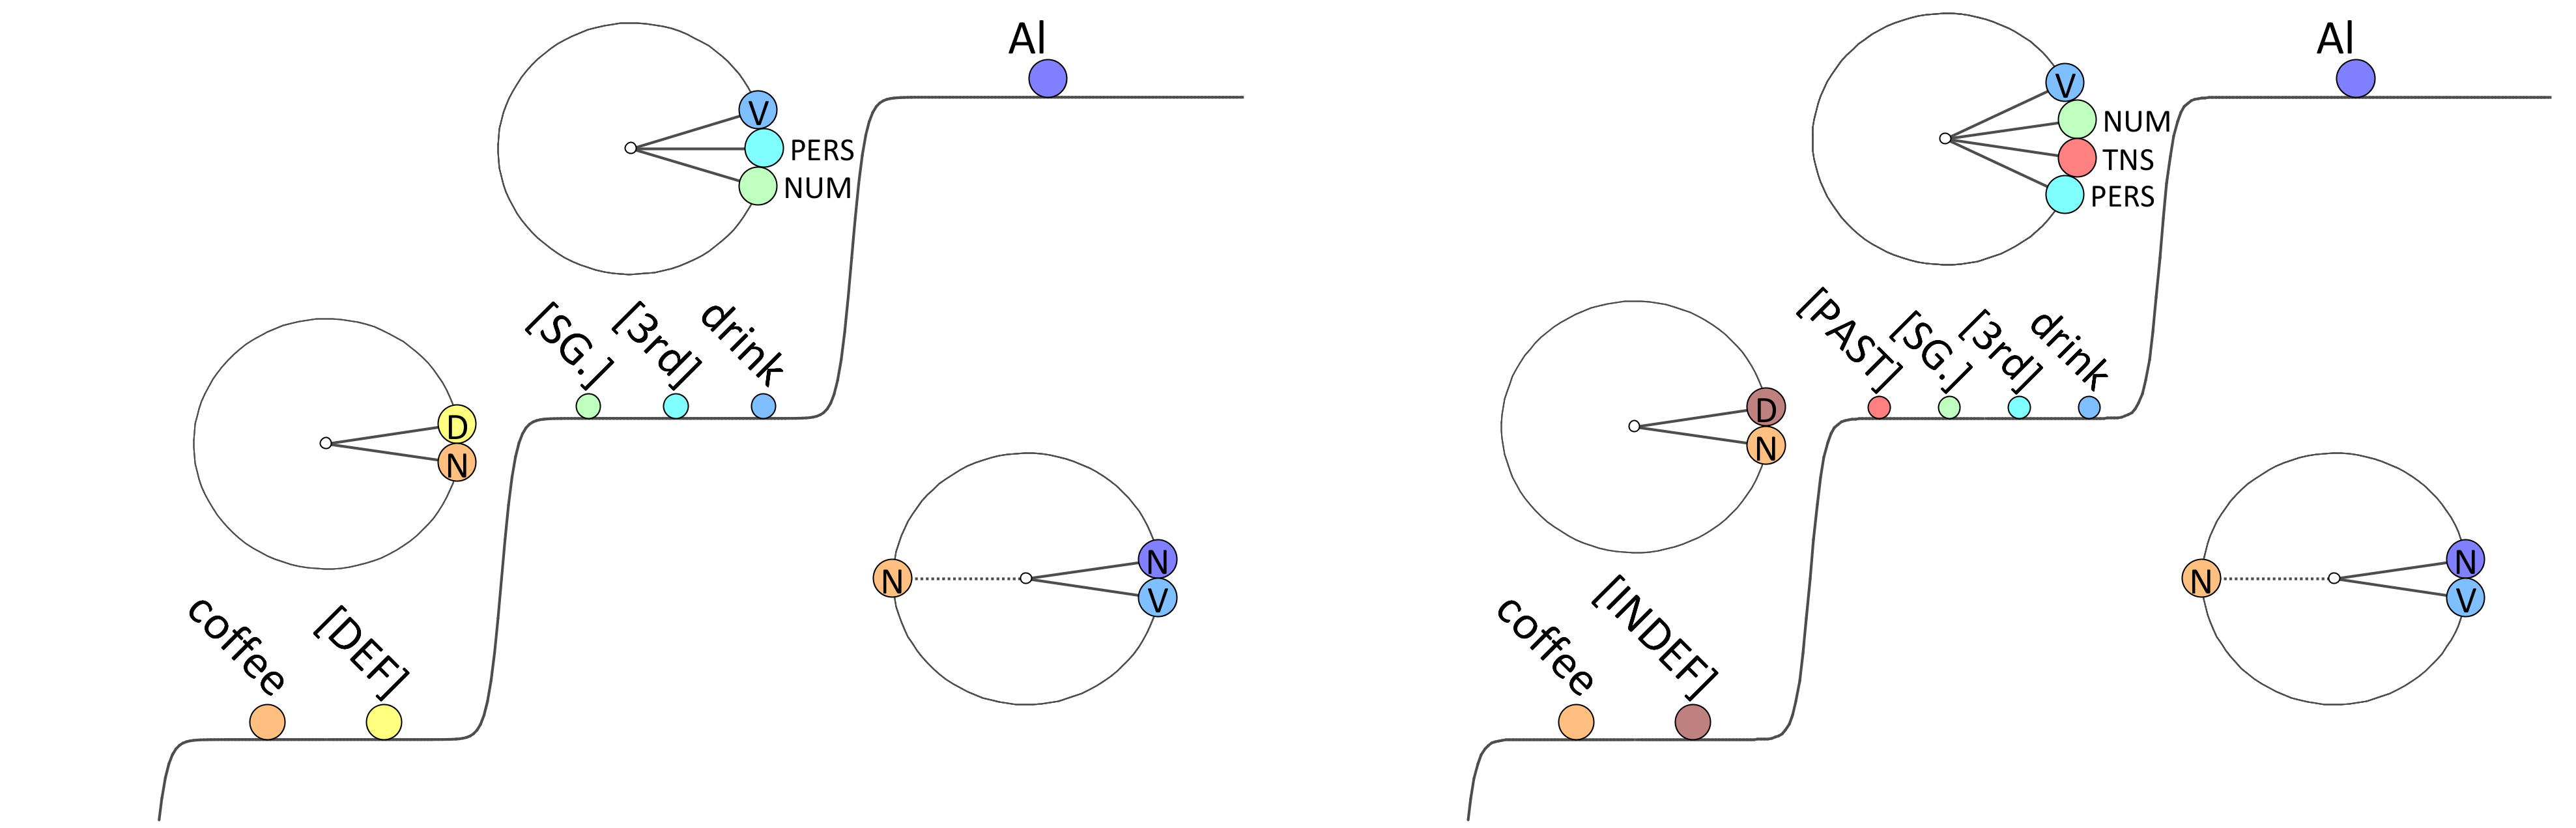
\includegraphics[width=\textwidth]{figures/Tilsen-img66.png}
\caption{\missingcaption}
\label{fig:4:16}
\end{figure}
 

\item  Grammatical s-systems are associated with a greater degree of population differentiation, particularly in highly inflected languages. In cases where subject nouns, object nouns, and verbs are inflected for some grammatical meaning, we analyze each inflectional marking as a distinct cs-resonance arising with differentiated grammatical s-systems. In the same way that the \{N\} population differentiates into \{-N\} and \{+N\}, inflectional s-systems can differentiate. In the analysis shown below, there are four s-system classes for number inflection: \{\textsc{number},+N\}, \{\textsc{number},-N\}, \{\textsc{number}{}-\textsc{V}\textsc{\textsubscript{+N}}\textsc{\}}, \{\textsc{number}{}-\textsc{V}\textsc{\textsubscript{{}-n}}\textsc{\};} we assume that all of these are differentiations of \{\textsc{number}\} and [\textsc{singular}]/[\textsc{plural}]. Because of the greater frequency of grammatical s-systems, differentiations of this sort can be more stable than those associated with lexical s-systems. 

  
\begin{figure}
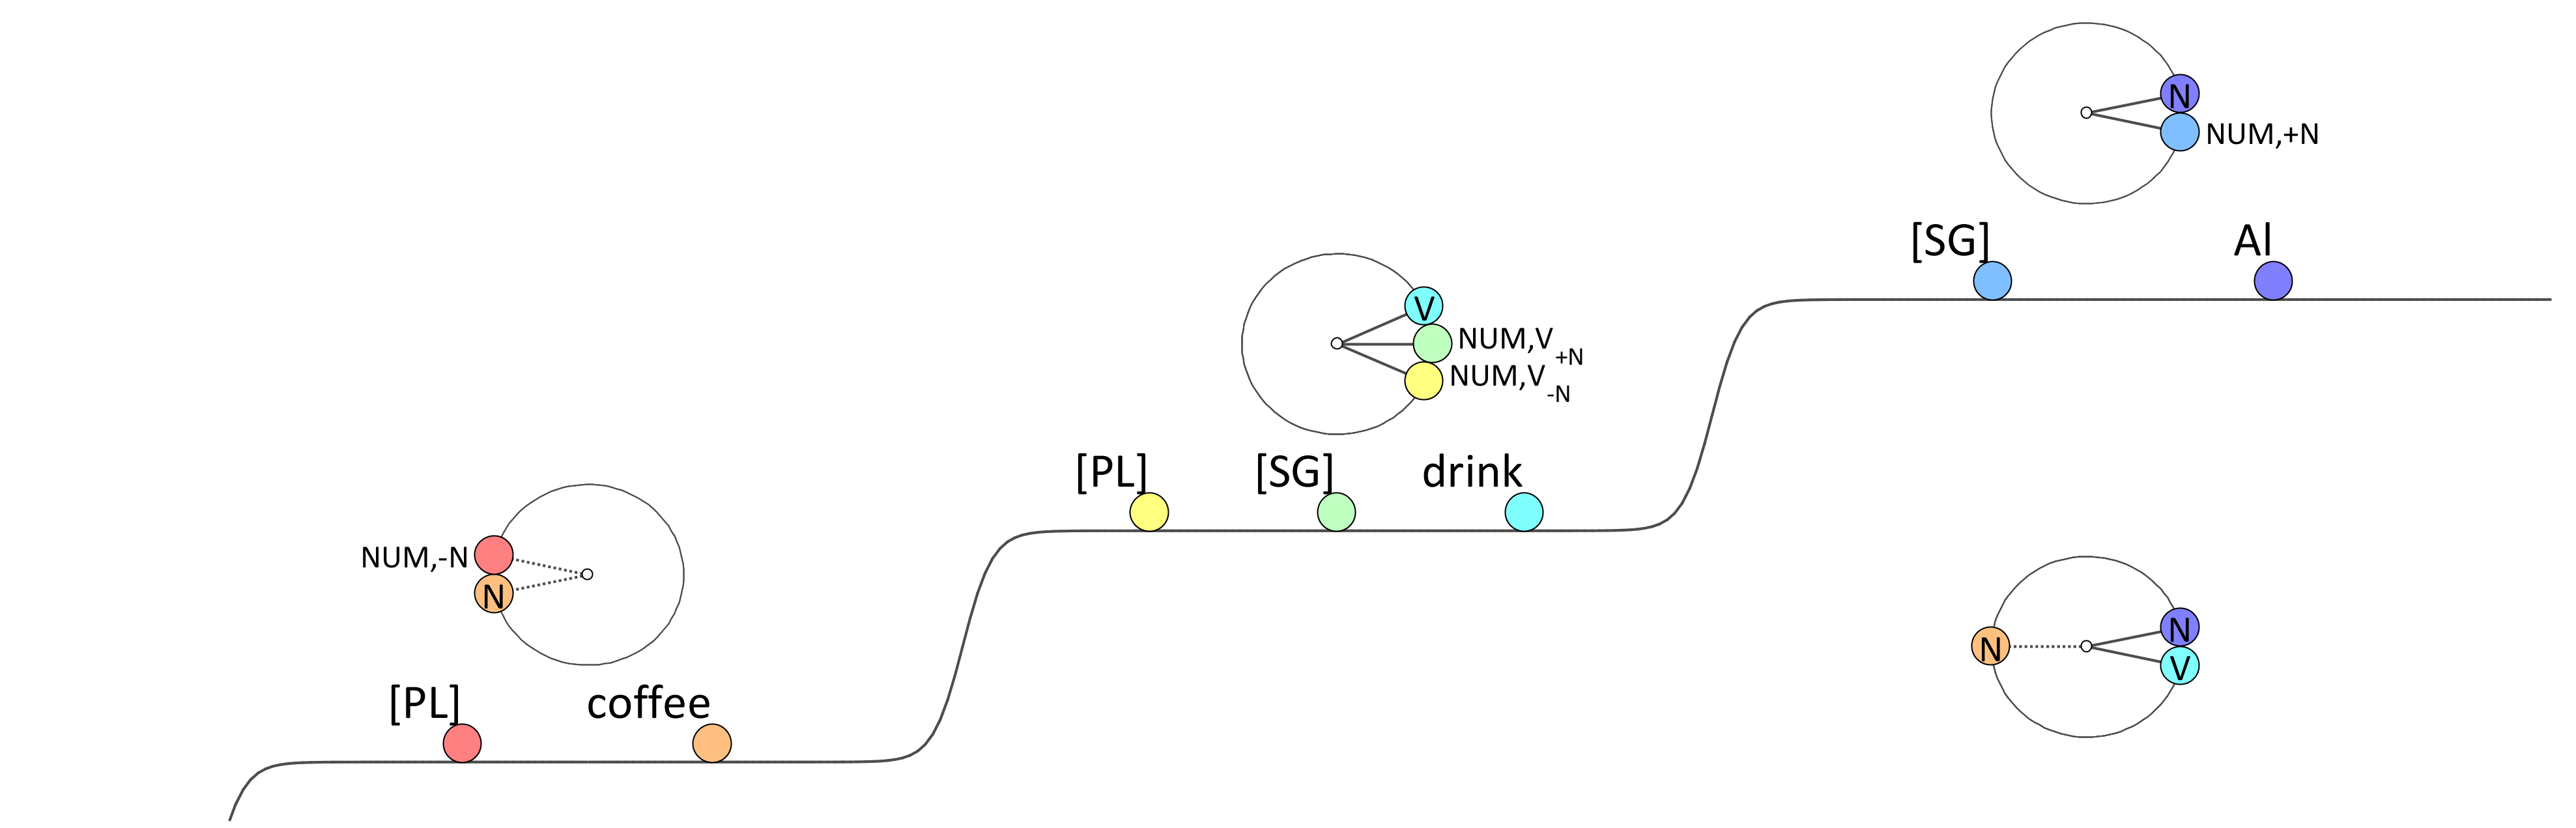
\includegraphics[width=\textwidth]{figures/Tilsen-img67.png}
\caption{\missingcaption}
\label{fig:4:17}
\end{figure}
\end{enumerate}
 

\subsection{Morphosyntactic and morphophonological status}

As a starting point for understanding the relation between cs- and gm-organization, we propose here a \textit{syntactic-motoric cotemporality hypothesis}. This hypothesis holds that, in a canonical trajectory, the gm-domain of a co-selected set of cs-systems in a given stable e-epoch is organized in that same epoch. This hypothesis reinterprets the notion of a “phonological word” (cf. \citealt{NesporVogel1986}, \citealt{Selkirk1984,Selkirk2011};: patterns associated with phonological words arise because all of the gm-systems associated with a set of co-selected cs-systems are organized into a stable e configuration in the same epoch. Another way of stating the hypothesis is to say that, in a canonical trajectory, excitation of the gm-domain of a cs-system neither occurs in an epoch prior to the selection of the cs-system nor is deferred to a subsequent epoch. There is thus a cotemporality of syntactic and motoric organization. 

  If the sm-cotemporality hypothesis holds, any apparent violations of sm cotemporality arise either from abnormal surroundings forces (i.e. constitute a non-canonical trajectory) or have been wrongly analyzed. The hypothesis is also consistent with the idea that each phonological word is associated with one accentual s-system \{\^{}\} and hence at most one [\textsc{accent}] system will be selected for each set of co-selected cs-systems. Cotemporality also leads to a reinterpretation of morphosyntactic distinctions such as affix/clitic, and bound/free morph. Many grammatical cs-systems are readily associated with one of just two morphosyntactic patterns, one affix-like, one clitic-like (see \citealt{Payne1997,Zwicky1985,ZwickyPullum1983} for further detail). To classify a cs-system [x]\{x\} along these lines we propose two criteria:

    (i)   [x]\{x\} must be co-selected with another system, [α]\{α\}.

    (ii)   [x]\{x\} is +φ-coupled to [α]\{α\}.

  A system which exhibits the affix-like pattern meets both criteria: the system is always co-selected with some other cs-system that it is +φ coupled to, i.e. a host system. Often the set of possible s-system hosts is small. For example, the nominal cs-system [\textsc{plural}]\{\textsc{number}\} is necessarily co-selected with \{N\}, and cannot be co-selected solely with other classes of lexical s-systems such as \{V\}, \{\textsc{adv}\}, \{\textsc{adj}\}. Another example is [\textsc{past}]\{\textsc{tense}\}, which is +φ coupled and co-selected with \{V\} or \{\textsc{aux}\}. Because an affix-like s-system is always co-selected with [α]\{α\}, the sm-cotemporality hypothesis entails that the gm-domain of [x]\{x\} is “phonologically bound” to the gm-domain of [α]\{α\}. 

  A system which exhibits the clitic-like pattern meets only criterion (i): the system is always co-selected with some s-system, but not necessarily one with which it is +φ-coupled. The set of possible s-system hosts is often larger than it is for affix-like systems. A consequence of failing to meet criterion (ii) is that clitic-like systems can participate in φ configurations with systems they are not co-selected with. For example, possessive \{\textsc{poss}\} is always +φ coupled to an \{N\} system, but can be co-selected with \{V\}, \{\textsc{adv}\}, or \{\textsc{adv}\}. Examples are shown in the {\tablebelow}.

\begin{table}
\begin{tabularx}{\textwidth}{p{1cm}Qp{1cm}Q}
\lsptoprule
\raggedleft \{N\} \par

\raggedleft \{V\}\par

\raggedleft \{\textsc{adj}\}\par

\raggedleft \{\textsc{adv}\} & \{\textsc{poss}\} co-selected with:

\textit{the coffee’s taste} 

\textit{the coffee Al drank’s taste}

\textit{the coffee that is cold’s taste}

\textit{the coffee Al drank yesterday’s taste} & \raggedleft \{N\}\par

\raggedleft \{V\}\par

\raggedleft \{\textsc{adj}\}\par

\raggedleft \{\textsc{adv}\} & \{\textsc{D}\} co-selected with:

\textit{the coffee}

\textit{the tastes good coffee}

\textit{the cold coffee}

\textit{the strongly brewed coffee}\\
\lspbottomrule
\end{tabularx}
\caption{\missingcaption}\label{tab:4:1}
\end{table}
\todo{redo this table with cells}

  Clitics and affixes are “bound” because they meet criterion (i). Some other grammatical cs-systems can be described as “free” because they meet a relaxed version of criterion (i) in which [x]\{x\} is \textit{usually} (rather than always) co-selected with another system. Determiners like \textit{a}, \textit{the}, and \textit{some}, are examples of cs-systems which are often but not necessarily co-selected with other systems. Specifically, these systems are often co-selected with \{N\}, sometimes with \{\textsc{adv}\} or \{\textsc{adj}\}, and yet can also be selected independently when a [\textsc{focus}] system couples to them (i.e. \textit{Al drank THE coffee}).

  Some example configurations are shown below. Observe that [the]\{\textsc{D}\} is in a φ configuration with [coffee]\{N\}, but is co-selected with [cold]\{\textsc{adj}\}. Likewise, [\textsc{poss}]\{\textsc{poss}\} is in a +φ configuration with [coffee]\{N\} and a -φ configuration with [taste]\{N\}, despite being co-selected with neither. 

  
\begin{figure}
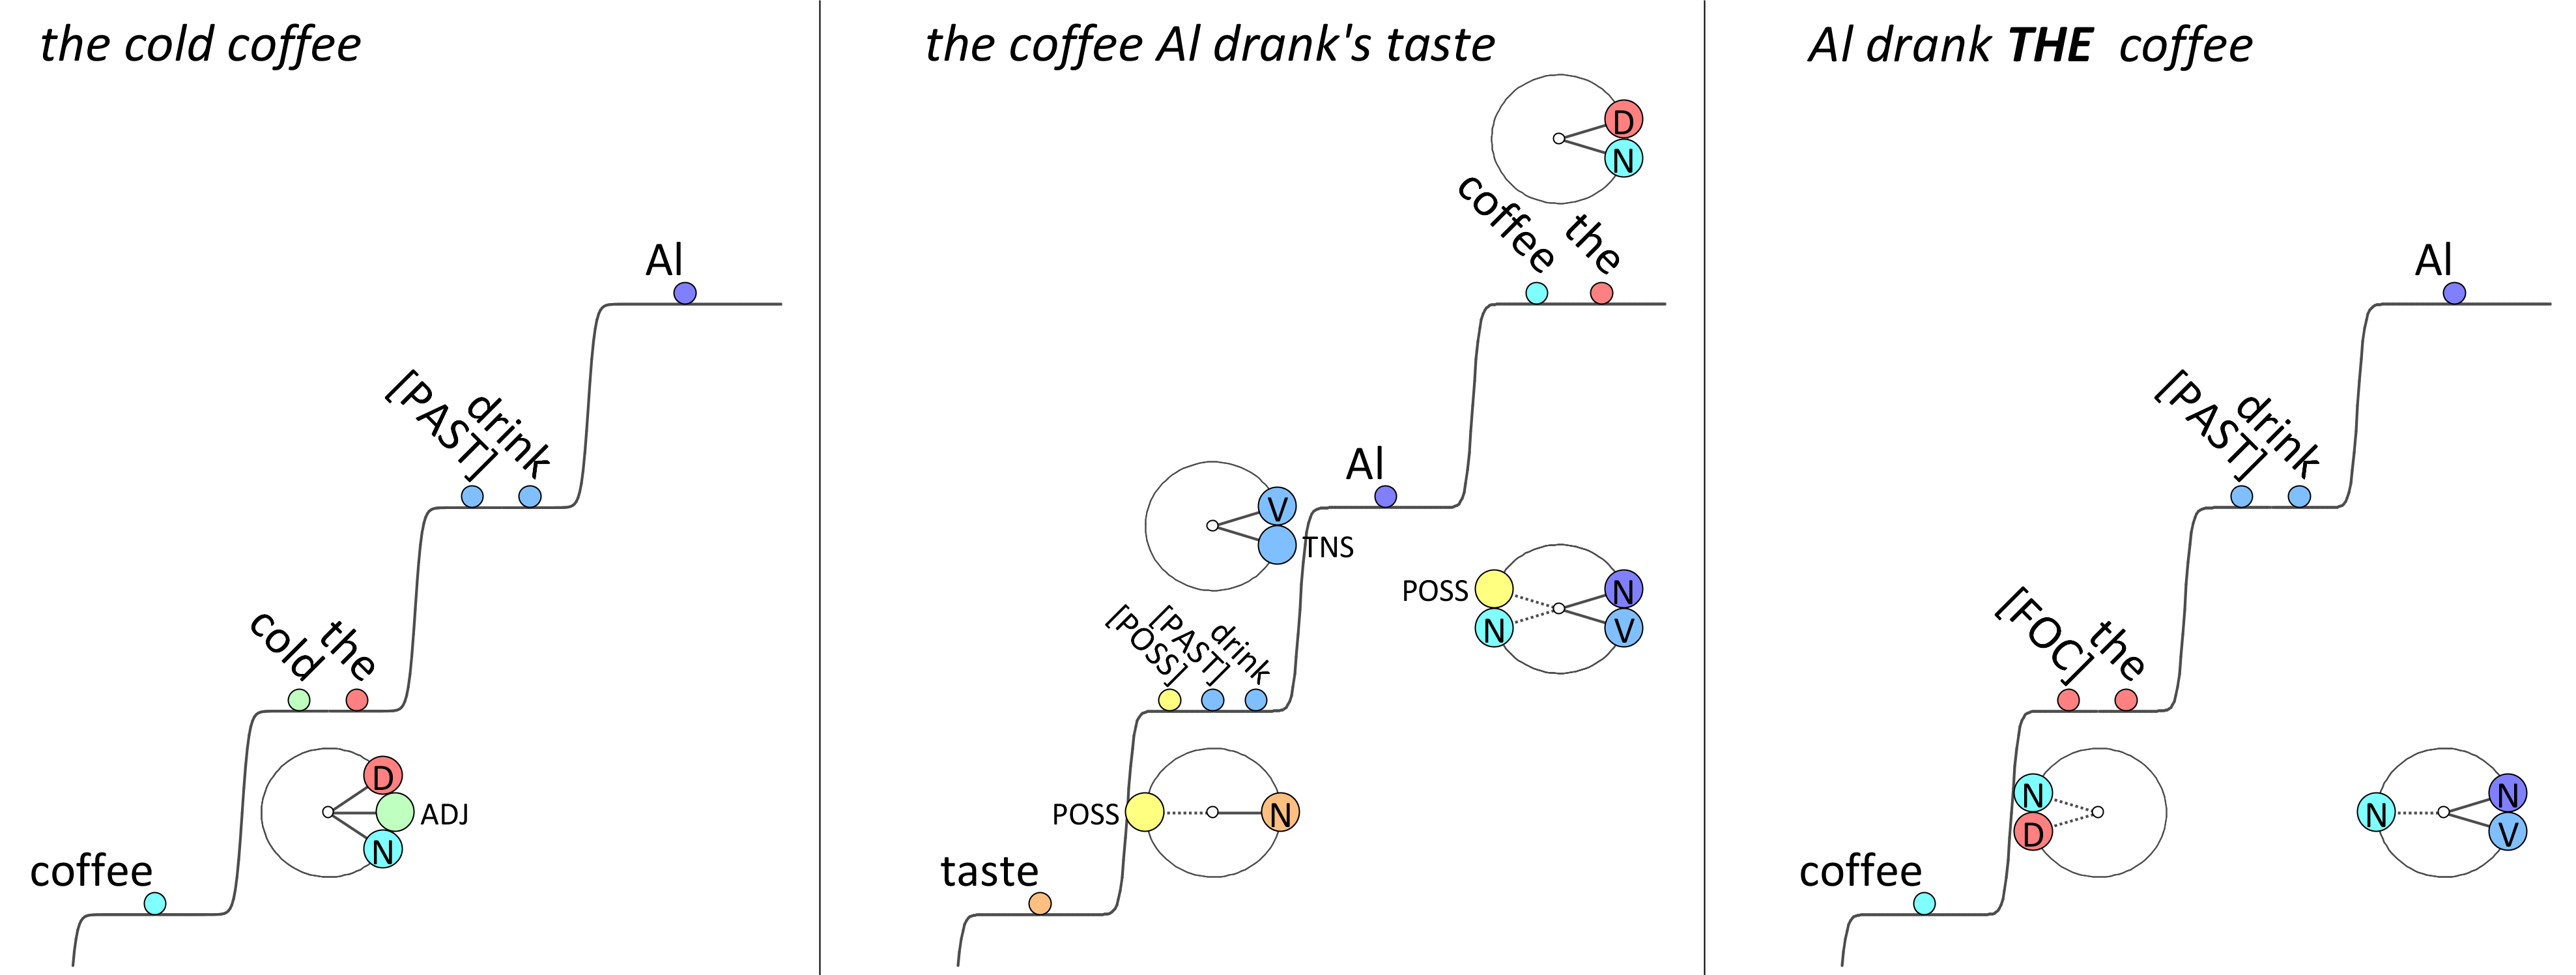
\includegraphics[width=\textwidth]{figures/Tilsen-img68.png}
\caption{\missingcaption}
\label{fig:4:18}
\end{figure}
 

  In the case of [\textsc{focus}], which is a subclass of [\textsc{accent}], we note that the distribution of [\textsc{focus}] coincides exactly with the set of possible co-selected systems. This suggests that [\textsc{focus}] resonates with any s-system which can be individually selected. These are often lexical s-systems like \{N\} and \{V\}, but can also be usually-but-not-always bound systems such as [the]\{DET\}. As shown above, with focus on the determiner, as in \textit{Al drank THE coffee}, [the]\{D\} occupies a level with a [\textsc{focus}] system, and we hypothesize that [\textsc{focus}] forms a cs-resonance with \{D\}. We assume that [\textsc{focus}] does not interfere strongly with the [\textsc{the}]\{D\} cs-resonance in this analysis.

  Instead of imposing classical categories of morphosyntactic status such as affix/clitic, and free/bound, a more sophisticated analysis aims to characterize degrees of combinatorial restriction on co-selection and the propensity of systems to φ-couple with co-selected systems (i.e. co-selective φ-coupling propensity). From this perspective we note that verbal inflection s-systems such as \{\textsc{tense}\} and \{\textsc{person}\} are more combinatorically restricted (these co-select only with \{V\} and \{\textsc{aux}\}) than \{D\} or \{\textsc{poss}\} (which co-select with a variety of lexical s-systems). The more restricted systems also have a greater co-selective φ-coupling propensity, i.e. they are more often co-selected with the system they φ-couple to. Further investigation of this correlation is warranted.

\subsection{State-dependence of gestural-motoric domains}

The canonical cs-to-gm mapping is one-to-one and does not depend on the states of other cs-systems. This means that each cs-system in a set of co-selected cs-systems drives the excitation of one gm-domain, whose composition does not vary as a function of the states of other cs-systems. This canonical scenario corresponds to prototypical agglutinative morphology. 

  Fusional morphs deviate from the canonical cs-to-gm mapping: their gm-domains depend on the cs-states of other systems. For example, the 3\textsuperscript{rd} person suffix of \textit{drinks} occurs only in the present tense. Co-selection of [drink]\{V\} with [\textsc{present}]\{\textsc{tense}\} and [\textsc{3}\textsc{\textsuperscript{rd}}]\{\textsc{person}\} excites an [alveolar narrow]\{-C\} gm-system (the suffix of \textit{drinks}), as shown in the example below. In contrast, co-selection of [drink]\{V\} with [\textsc{present]}\{\textsc{tense}\} and [\textsc{1}\textsc{\textsuperscript{st}}]\{\textsc{person}\} does not excite the [alveolar narrow]\{-C\} system. A strong hypothesis is that cs-to-gm mappings can depend only on selected cs-systems. In other words, the gm-systems which are organized in a given epoch cannot depend on cs-systems which are not selected in that epoch. For instance, fusional cs-to-gm mappings associated with inflection of \textit{drinks} in the utterance \textit{Al drinks coffee} cannot depend on [Al]\{+N\} or [coffee]\{-N\} (of course, the selection of grammatical cs-systems can depend on contemporaneously organized system). This strong hypothesis may follow as a consequence of sm cotemporality; it makes sense because fusion arises from gestural overlap, and such overlap is expected to be more extensive among gestures which are contemporaneously organized. Whether the hypothesis needs to be weakened such that cs-to-gm mappings can depend on all excited cs-systems, not just the selected ones, is an open question.

  
\begin{figure}
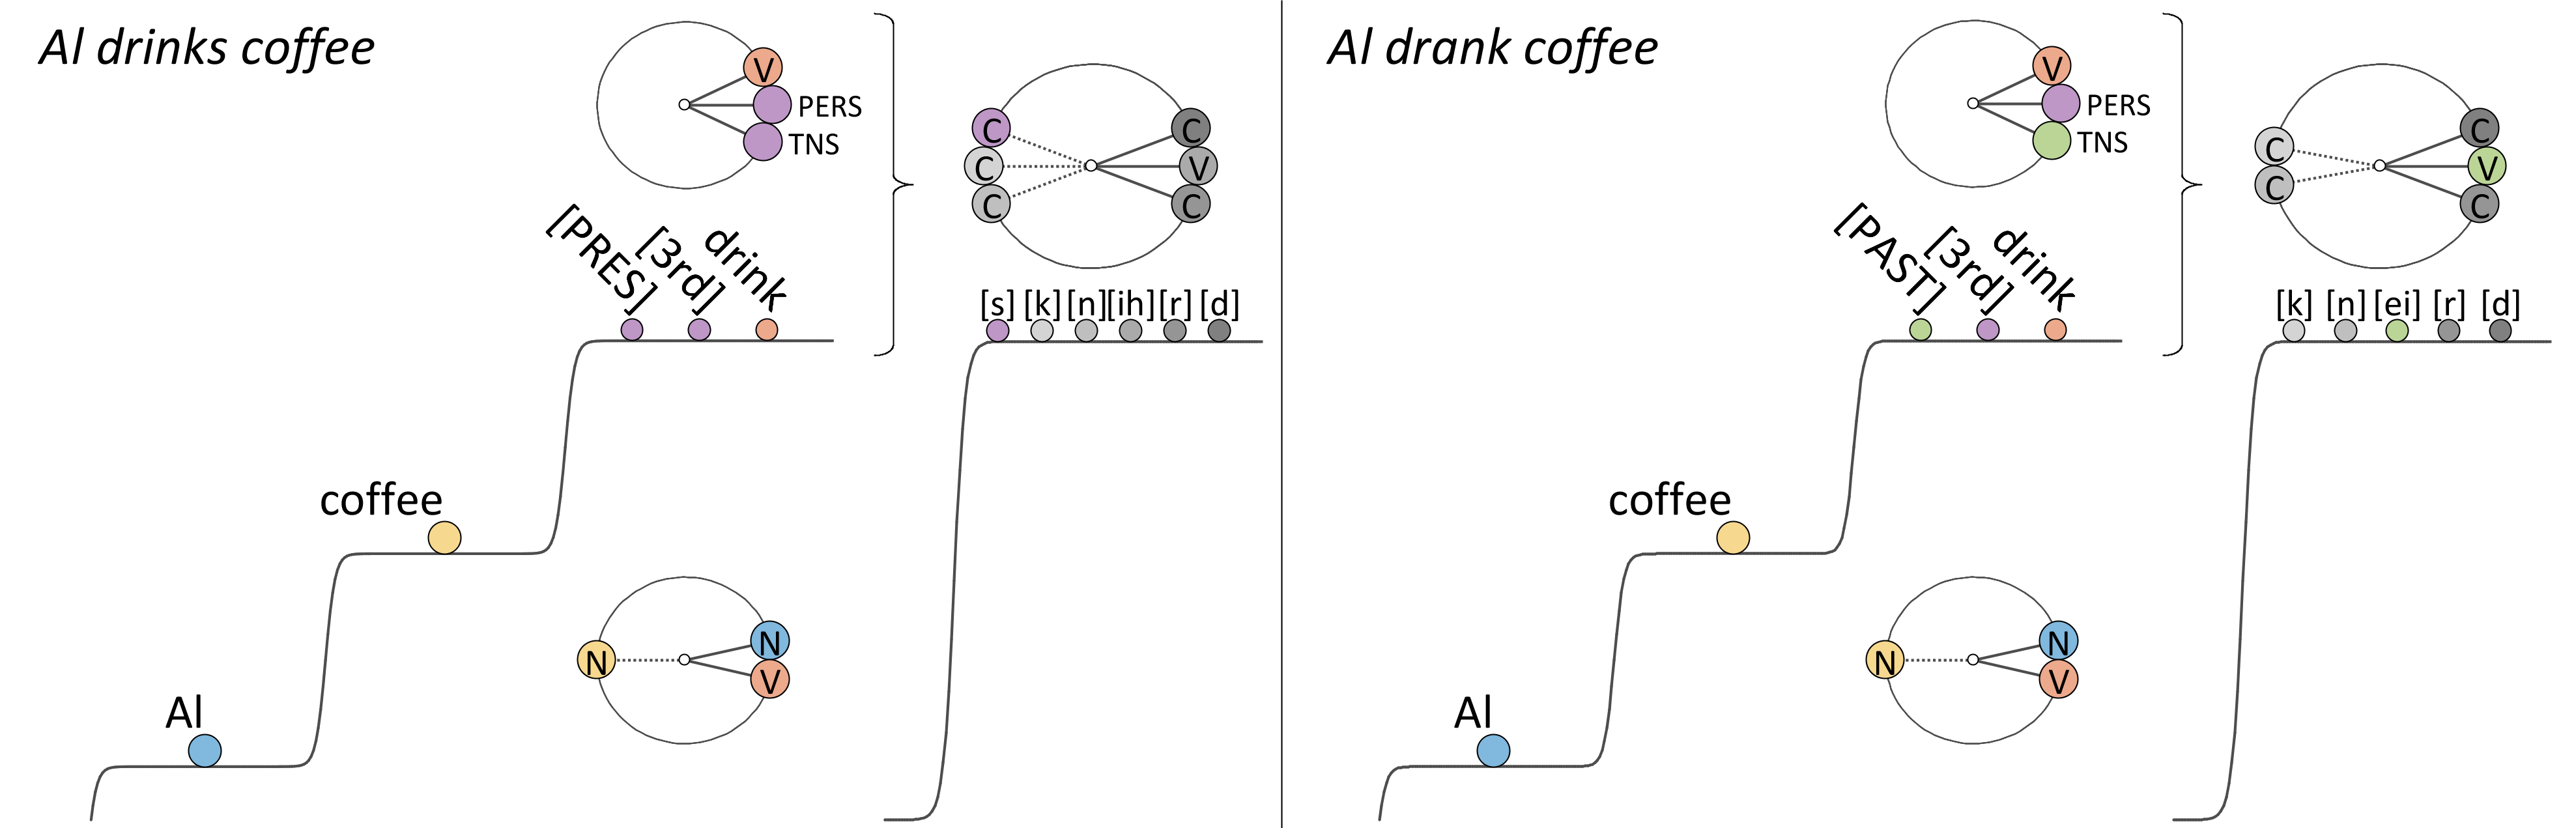
\includegraphics[width=\textwidth]{figures/Tilsen-img69.png}
\caption{\missingcaption}
\label{fig:4:19}
\end{figure}
 

  Suppletive morphological patterns are similar to fusional ones, except that a suppletive gm-domain depends on the identity of the \textit{lexical} c-system. For example, a weakly suppletive allomorphy such as ablaut of \textit{drank} /dreink/ is shown above. In a state with [drink] and [\textsc{past}] selected, a different vocalic gesture is excited than the one that is excited in the state where [drink] and [\textsc{present}] are selected. In other words, the cs-to-gm mapping of [drink] differs depending on which [\textsc{tense}] system is selected. Strongly suppletive allomorphy, e.g. \textit{Al goes for coffee} vs. \textit{Al went for coffee}, exhibits the same dependence of gm-domain on the identity of selected lexical and grammatical c-systems, but the differences in gm-domains are greater.

\subsection{Derivational vs. inflectional morphology}

A commonly employed distinction in morphological analysis is one between derivational and inflectional morphology (\citealt{BickelNichols2007,Booij1996,Dressler1989,HaspelmathSims2013}). The qualities which are used to distinguish derivational and inflectional morphology—i.e. productivity, compositionality of meaning, and free vs. bound status—must be characterized by statistical analysis over a corpus of utterances. This assumes some particular spatial and temporal scales associated with the corpus, and is not always generalizable. 

  For example, roots like \textit{cran} in \textit{cranberry} are only “bound” to the extent that our analysis finds that these systems are infrequently selected without another lexical system. But if we observe that speakers produce forms such as \textit{cran-grape} and \textit{cran-apple}, and readily make sense of utterances like \textit{Al is a big fan of cran}, then we infer that there is a [cran] c-system, and that [cran] can couple to \{N\} productively. The irony is that when we refer to “cran” as a bound morph in an analytical context, we promote the independent selection of this cs-system, in a statistical sense. Thus people with some instruction in morphology may be more likely to productively couple bound morphs that were exemplified as such, and this in turn makes those morphs more likely to be exhibit the distributional patterns of free morphs! This irony highlights the fact that our use of the terms “bound” and “free” depend on a choice of analytical scale.

  Indeed, some “derivational” morphology is, contrary to prototype, very productive. In some languages intransitive \{V\} systems can be transitivized. The lexicalized transitivity contrast in English between c-systems [die] and [kill] is associated with an affix-like system in some languages, i.e. \textit{make-die}. Such patterns can be readily analyzed as co-selection of verbal cs-system [die]\{V\} and a transitivizing or causativizing cs-system, [\textsc{cause}]\{\textsc{valency}\}. Derivational cs-systems of this sort are akin to much of the inflectional morphology we examined above. 

  Given the complexity and scale-dependence of the relevant factors, we should be careful to avoid imposing a categorical distinction between derivational and inflectional morphology. Instead, we should interpret productivity, compositionality, and boundedness as statistical descriptions of patterns of organization, which necessarily require a choice of spatial and temporal scales. From this perspective it would be a worthwhile endeavor to re-examine the generalization that derivational morphology “precedes” inflectional morphology \citep{Booij1996}.

\subsection{Case marking}

All of the s-systems we have constructed so far have been associated with one or more c-systems, and our assumption has been that these s-systems, whether lexical or grammatical, become active through resonance with c-systems. However, there is no a priori reason to rule out the possibility that s-systems might be activated through interactions with other s-systems, or require combinations of s-system and c-system coupling to be activated. Case marking appears to be a phenomenon of this sort (\citealt{BobaljikWurmbrand2008,MalchukovSpencer2008}).

  Here we hypothesize that some forms of case marking involve \{\textsc{case}\} s-systems which become active through interactions with other s-systems. First, note that case marking systems are cross-linguistically diverse \citep{MalchukovSpencer2008}. One puzzle that we must address is this: although some case marking patterns are predictable from φ configurations (i.e. relational meaning), many appear to be correlated with an initial e configuration. Various common case marking patterns are schematically arranged below. 

  
\begin{figure}
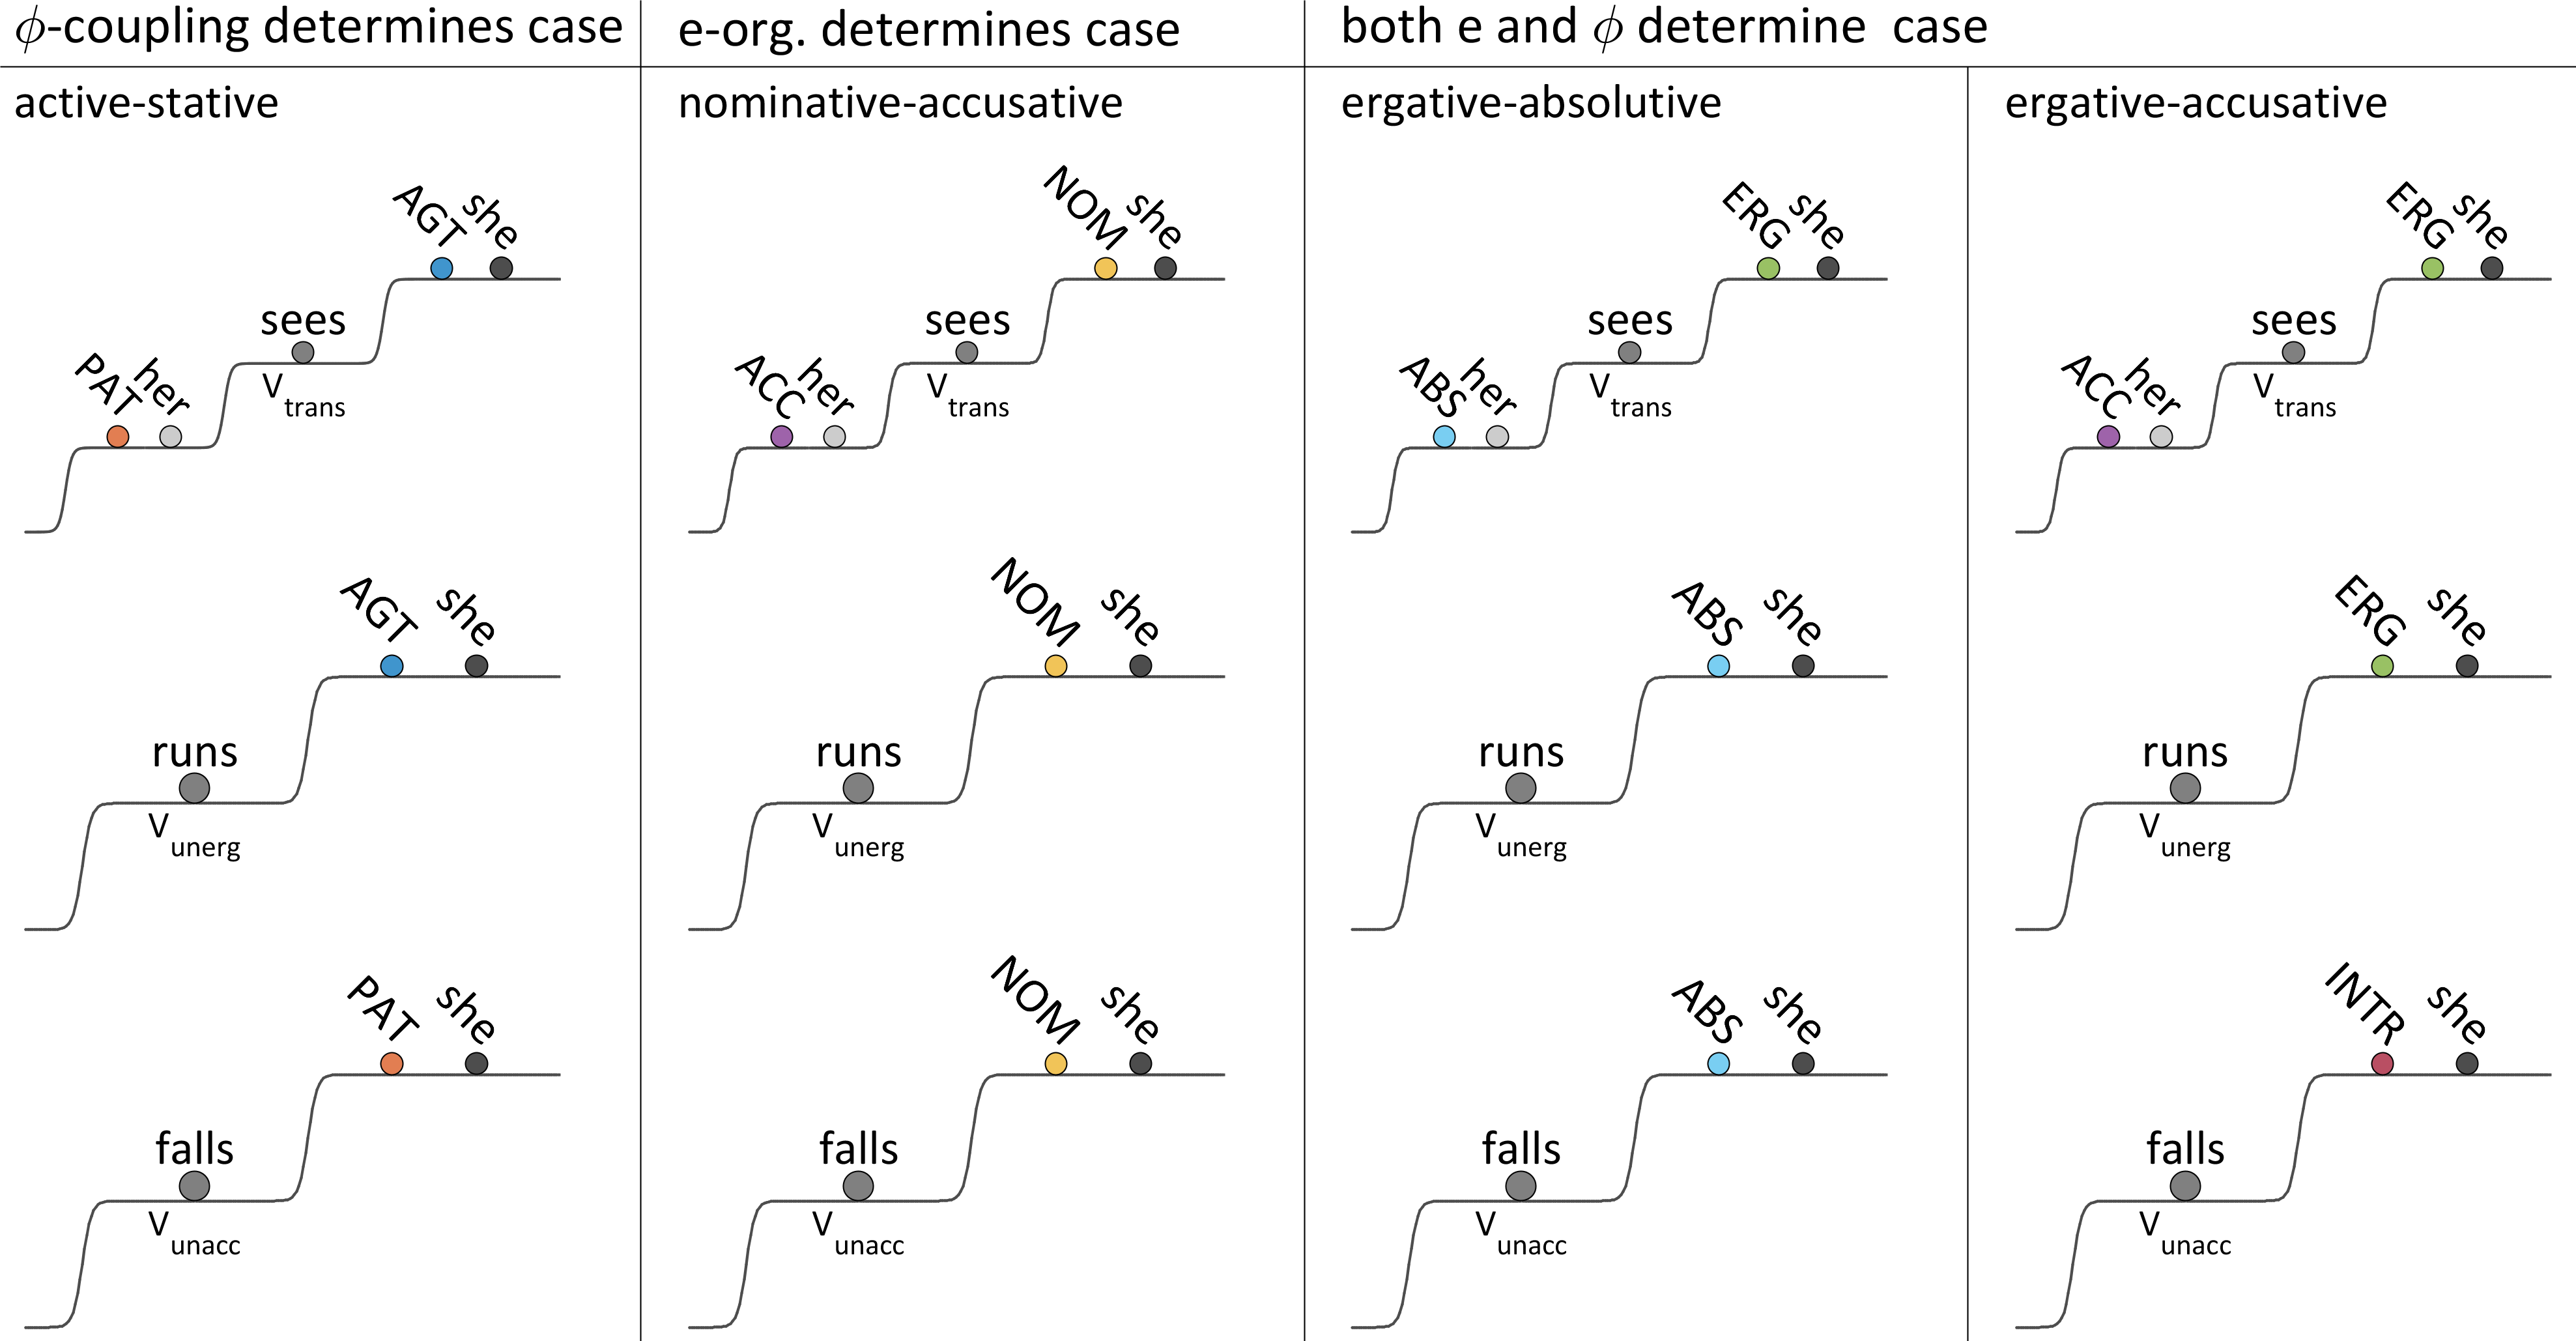
\includegraphics[width=\textwidth]{figures/Tilsen-img70.png}
\caption{\missingcaption}
\label{fig:4:20}
\end{figure}
 

  The pattern in which φ-coupling solely determines case corresponds to active-stative marking: \{+N\} arguments are coupled with [\textsc{agent}]\{\textsc{case}\} and \{-N\} arguments are coupled with [\textsc{patient}]\{\textsc{case}\}. The pattern in which e-organization solely determines case corresponds to nominative-accusative case marking: an \{N\} argument in some e-level defined relative to \{V\} couples with [\textsc{nominative}]\{\textsc{case}\}, and \{N\} arguments in some other e-level relative to \{V\} couple with [\textsc{accusative}]\{\textsc{case\}}. In English, [\textsc{nominative}]/[\textsc{accusative}] are mapped to \{N\} in levels above/below \{V\}, respectively. The specific mapping will of course differ according to basic word order of a language. Ergative-absolutive is a pattern in which both e- and φ-organization determine case marking: \{+N\} arguments couple to [\textsc{ergative}]\{\textsc{case}\} when the e configuration involves two arguments, but when the e configuration has just one argument, \{N\} couples to [\textsc{absolutive}]\{\textsc{case}\}.

  Case typically develops diachronically from adpositions (\citealt{Heine2009,TraugottHeine1991}) which relate \{N\}-coupled c-systems to other \{N\}- or \{V\}-coupled c-systems, and so we expect semantic regularities in cases. We have hypothesized that \{\textsc{case}\} s-systems are special because they \textit{may} become excited through interactions with other s-systems, or through combinations of s- and c-system states. This predicts that \{\textsc{case}\} excitation can be fully or partly dissociated from relational meaning, and instead can become associated entirely with e-organization. Perhaps \{\textsc{case}\} systems can become dissociated from relational meaning because they are redundant, particularly in languages with relatively fixed word order. This perspective provides a new basis for understanding the typological diversity of case marking systems, and also provides insight into some of the interesting “structural” patterns which have been conventionally associated with case. 

  One observation that is important to conventional theories of case is that non-finite verbs cannot assign case to subjects (i.e. nominative case, see \citealt{Chomsky1980,ChomskyLasnik1977,Vergnaud2006}). Hence \REF{ex:4:1a} below is judged unacceptable because the utterance-initial pronoun cannot be assigned case. In contrast, \REF{ex:4:1b} is acceptable because the finite verb \textit{drinks} can assign the pronoun case, and \REF{ex:4:1c} is acceptable because the preposition \textit{for} can assign case (here accusative).

\ea
  \ea[*]{\label{{ex:4:1a}}He to drink coffee would be good.}

  \ex[]{\label{ex:4:1b}That he drinks coffee would be good.}

  \ex[]{\label{ex:4:1c}For him to drink coffee would be good.}
\z
\z

  In the o/el framework we reinterpret case as potentially determined by e-organization (or, interactions between s-systems), in a language-specific way, and hence we infer that the organization in \REF{ex:4:1a} is not a context in which [\textsc{nom}]\{\textsc{case}\} can resonate with \{V\} and \{N\}. The important question is why. The inclusion of a non-finite [\textsc{inf}]\{i\} system appears to be responsible. Instead of understanding the unacceptability of \REF{ex:4:1a} as the result of a restriction on the “ability” of verbs to “assign case,” we reconceptualize the pattern as a trajectory in which [\textsc{nom}]\{\textsc{case}\} does not become excited, and note that such trajectories occur when [\textsc{inf}]\{i\} is excited. This suggests some form of interaction between [\textsc{inf}]\{i\} and [\textsc{nom}]\{\textsc{case}\}, the basis of which warrants further investigation.

  One of the more interesting patterns involving case is the exceptional case marking pattern, which is illustrated by examples in \REF{ex:4:2}. Some verbs, like \textit{believe}, can assign case to the subject of the non-finite verb in a complement clause, but others, like \textit{decide}, cannot. Contrasts such as these show that although \{\textsc{case}\} s-systems can be excited via interactions with s-systems, their excitation may depend also on the identities of excited c-systems. In \REF{ex:4:2a} we see that \textsc{[acc]\{case\}} is excited by a [believes]\{V\} system, even though \textsc{[acc]\{case\}} is not coupled with any system that is coupled to [believes]\{V\}. The same does not occur with [decides]\{V\}. The passive in \REF{ex:4:2d} provides another example: the pronoun is marked with nominative case, presumably because [\textsc{nom}]\{\textsc{case}\} is excited by resonance with [\textsc{he}]\{N\} and [\textsc{be}]\{\textsc{aux}\}.

  \ea\label{ex:4:2}
  \ea[]{\label{ex:4:2a}Bo believes him to drink coffee}
  \ex[*]{Bo decides him to drink coffee}
  \ex[]{Bo decides that he drinks coffee}
  \ex[]{\label{ex:4:2d}He is believed to drink coffee by Bo.}
  \z
  \z
  Although we have not attempted to develop a comprehensive theory of case in the current framework, the basis of such a theory is expected to derive from the hypothesis that \{\textsc{case}\} s-systems have the atypical property of potentially being activated and excited solely by interactions with other s-systems. This property is what appears to underlie the typological diversity of case patterns. 

\section{Phrasal organization}

According to the principle of relational meaning, relational meaning experiences are stable relative phase configurations. What more can we say regarding these φ configurations, and how do φ and e configurations interact? Below we propose a general principle and consider several specific hypotheses regarding φ/e configurations associated with phrasal organization. We then apply these to various patterns of phrasal organization, i.e. arguments, adjuncts, ditransitive and passive constructions, etc. The proposed principle is as follows:

\textit{The principle of} φ configuration \textit{invariance}: 

  All classes of relational meaning map invariantly to either +φ or -φ configurations. 

  The φ configurational invariance principle holds that there are only two types of stable configurations, +φ and -φ, and that for any given class of relational meaning, instances of that class always arise from the same type of configuration or combination of types. Moreover, the syntactic mechanism for stabilizing φ configurations is cs-resonance in combination with s-s coupling, where all s-s coupling is either +φ or -φ. \textit{Classes} of relational meaning are therefore associated with patterns of s-system coupling. We propose two hypotheses which specify how the φ configuration invariance principle is instantiated:
  
\begin{enumerate}
\item The following semantic relations are always -φ configurations:
\begin{enumerate}
  \item \{V\} and patient/theme/goal \{N\}
  \item preposition \{P\} and complement \{N\}
  \item possessor \{N\} and possessed \{N\}
\end{enumerate}
\item  All other semantic relations are +φ configurations.
\end{enumerate}

  In applying these hypotheses to various patterns of phrasal organization, we reach several general conclusions. First, [-] valence φ coupling is special; the majority of φ relations in our analyses have [+] valence. Second, \textit{e} organization is not necessarily contingent on φ organization, even in languages with relatively fixed word order such as English. Third, the conventional notion of \textit{obligatoriness} is untenable and must be replaced with a measure of state space volume. Fourth, there are inherent limits on the number of systems which can be excited simultaneously, because of interference between systems. For exposition we use terminology which refers to semantic roles, e.g. agent/experiencer, patient/theme, location/recipient, etc. to describe relational meaning experiences; we do this for convenience, not because these roles are theoretically presupposed.

\subsection{The principle of \textup{φ configuration} invariance and configurational hypotheses}

For relational meanings with verbal flavor (i.e. actions/events/states), agent/experiencer-relations arise from +φ coupling between \{N\} and \{V\}, and patient/theme-relations from -φ coupling between \{N\} and \{V\}. There are two general possibilities for mapping argument roles to configurations: (i) role-to-φ invariance and (ii) e-to-φ invariance. Here we consider both (i) and (ii), but argue for the former, which holds that semantic roles map invariantly to φ-configurations. Initial configurations are shown below for intransitive and transitive verbs in the invariant role-to-φ scheme. The patient [Bo] has a -φ relation to the verbal concepts in both intransitive [died] and transitive [killed] utterances. As a consequence of this, the \{-N\} system occupies a different e-level relative to \{V\} in intransitive and transitive configurations. In other words, φ-to-e mapping is not invariant in this scheme.

  
\begin{figure}
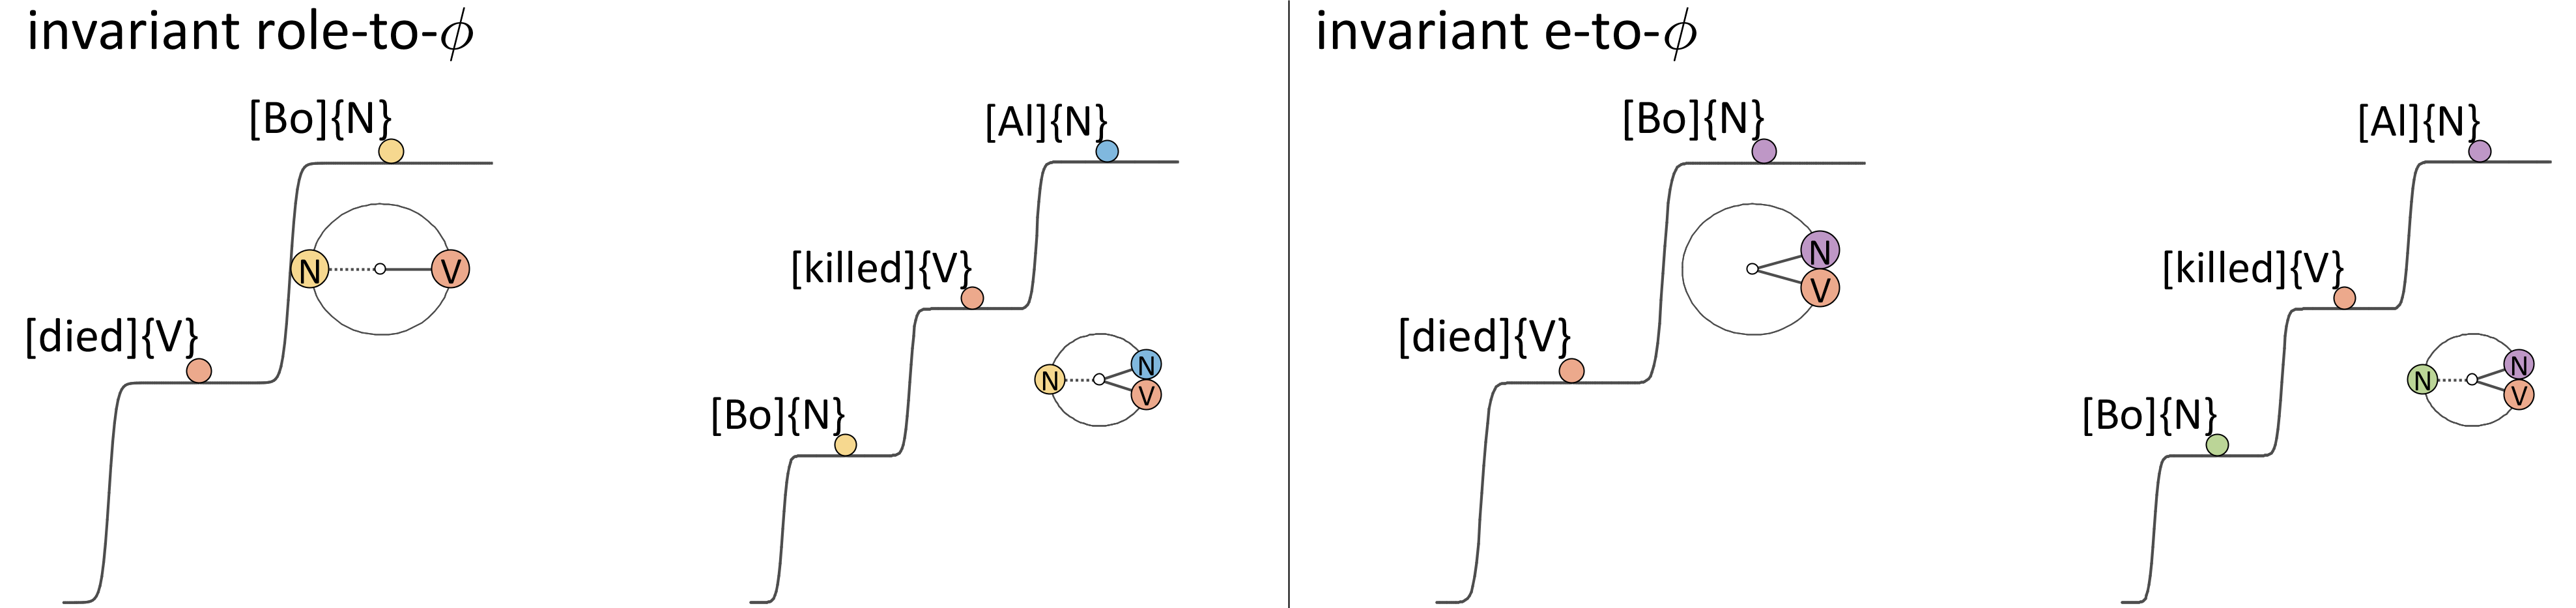
\includegraphics[width=\textwidth]{figures/Tilsen-img71.png}
\caption{\missingcaption}
\label{fig:4:21}
\end{figure}
 

  The alternative scheme (which we argue against) maps initial e-organization invariantly to φ configuration, in which case +φ and -φ coupling relations correspond to e-levels relative to \{V\}, i.e. subject/argument positions. In the invariant e-to-φ scheme, φ relations are predictable from relative e-level. In English, this maps a thematic/patient argument of an intransitive verb such as \textit{died} to a +φ configuration with \{V\}, violating the principle of φ configurational invariance.

  Why should we prefer role-to-φ invariance over e-to-φ invariance? The main reason is that invariance of some sort must exist to provide a universal basis for relational meaning experiences. If relational meaning were determined directly by e-organization, we would expect word order to be equally important across languages, and possibly the same in all languages. The fact that many languages have relatively free or variable word order, and that basic word orders differ across languages, suggests that e-to-φ invariance is not the primary mechanism for regulating relational meaning. 

  A consequence of preferring role-to-φ invariance is that e-organization is not necessarily predictable from φ configuration, and this entails that we need to consider language-specific and contextual (i.e. surroundings-contingent) influences on e-organization. For example, how should we conceptualize differences between intransitive and transitive verb systems, as in \textit{died} vs. \textit{killed} above? Consider that what we write in []-brackets is merely a label for a c-system, and not of theoretical interest. However, by using two different labels as above, we implicitly have constructed distinct c-systems, [die] and [kill]. An alternative is to propose a generic [die] c-system for both \textit{die} and \textit{kill}, and to and make use of some other class of systems to account for the transitivity difference. The utility of this approach is more obvious when we consider verb forms which can be intransitive or transitive, e.g. [break] in \textit{windows broke} vs. \textit{Al broke windows}. 

  The representations below contrast four possible analyses, which arise from crossing two different hypotheses. (A/A') differentiate intransitive \{V\textsubscript{IN}\} and transitive \{V\textsubscript{TR}\} s-systems. (B/B') posit a valency \{\textsc{val}\} s-system and differentiates between [\textsc{intransitive}]\{\textsc{val}\} and [\textsc{transitive}]\{\textsc{val}\} systems. Hence the contrast between A/A' vs. B/B' amounts to whether we differentiate \{V\} into two subclasses of \{V\}: \{V\textsubscript{IN}\} and \{V\textsubscript{TR}\}, or construct a new class, \{\textsc{val}\}.

  
\begin{figure}
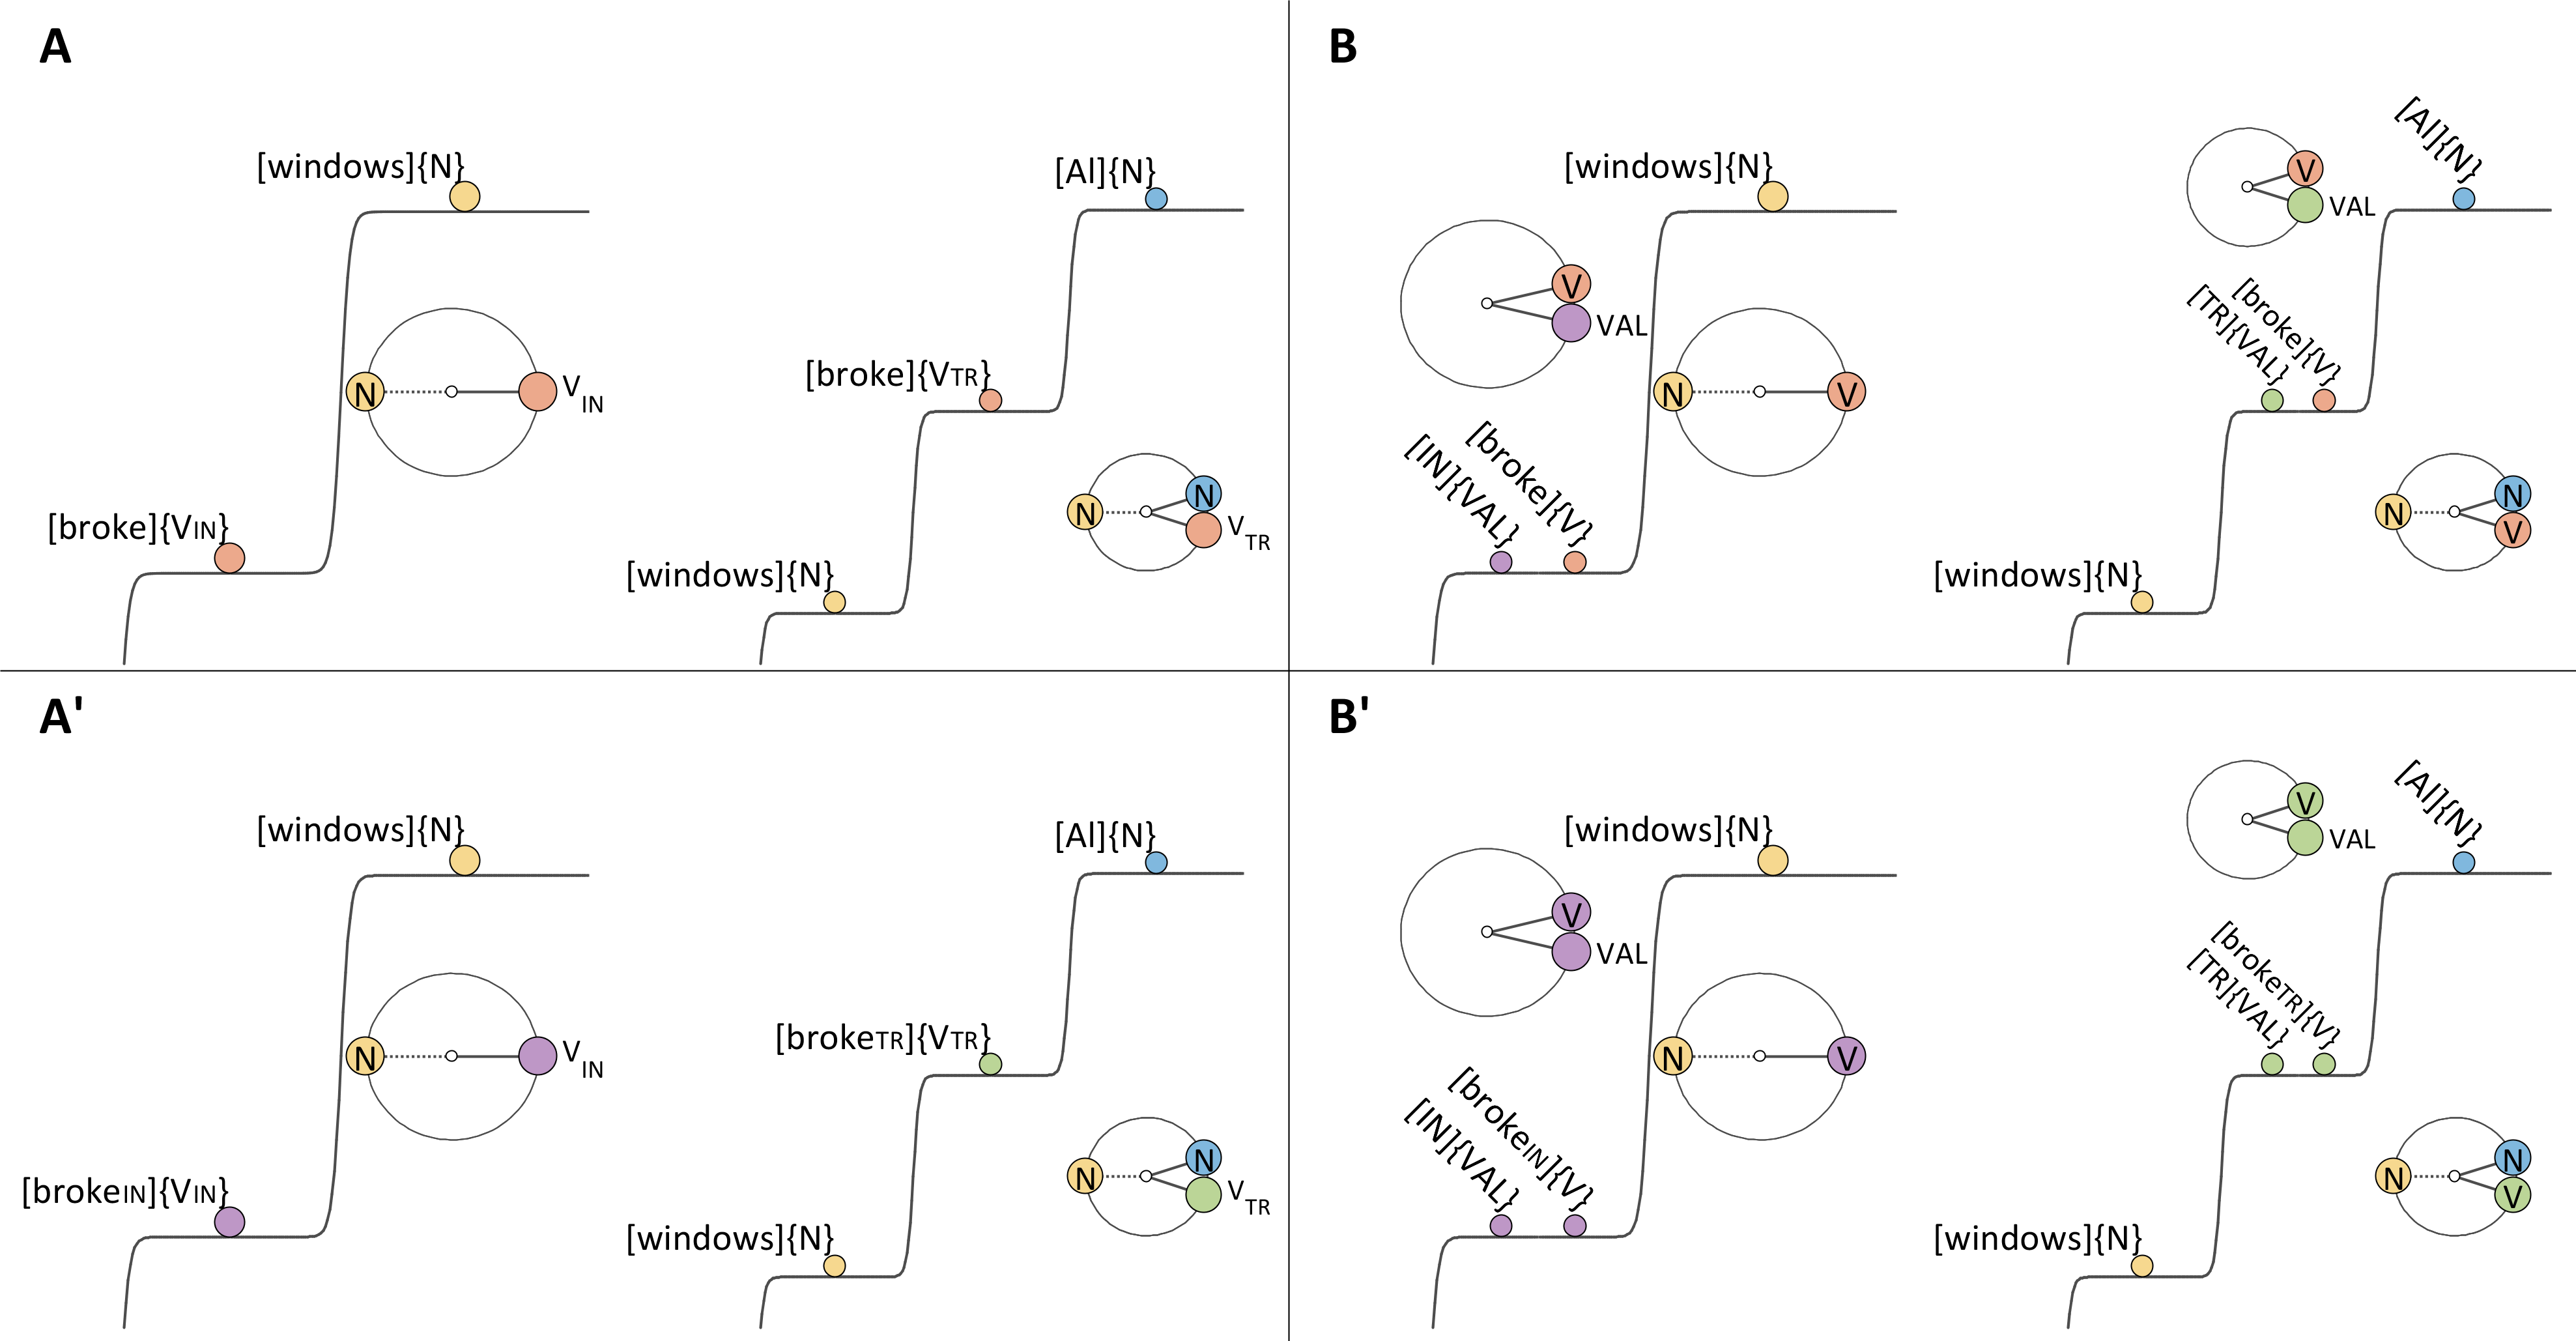
\includegraphics[width=\textwidth]{figures/Tilsen-img72.png}
\caption{\missingcaption}
\label{fig:4:22}
\end{figure}
 

  The contrast between (A,B) and (A',B') is whether we differentiate [break] into two distinct c-systems. In (A,B) there is only one verbal c-system, [break]; in (A',B') there are two distinct c-systems, [break\textsc{\textsubscript{tr}}] and [break\textsc{\textsubscript{intr}}]. Moreover, A/A' and B/B' are not mutually exclusive, because we can differentiate \{V\} into \{V\textsubscript{IN}\}/\{V\textsubscript{TR}\} systems \textit{and} proliferate a new s-system class, \{\textsc{val}\}. This doubles the number of possible analyses to eight. If we consider analyses in which there is no differentiation of \{V\} nor a \{\textsc{val}\} system, we have sixteen possibilities. Which of these should we prefer? 

  One consideration is that initial e-organization can be influenced by transitivity in some languages. Since e-organization is most directly a result of s-system interactions, we might infer that there must be some s-system manifestation of valency; this manifestation could be \{V\} differentiation and/or a \{\textsc{val}\} system. Furthermore, there must be a c-system manifestation of transitivity, because without one there would be no basis for a difference in meaning experience. The question then becomes whether we should differentiate verbal concepts (i.e. [break\textsc{\textsubscript{intr}}] and [break\textsc{\textsubscript{tr}}]) and/or construct new c-systems, (i.e. posit [\textsc{intrans}] and [\textsc{trans}])?

  When we consider our microscopic model, the difference between these options is not so clear. On the microscale, similarity in meaning experiences on supra-utterance timescales is understood as similarities in the synaptic interactions a concept population has with other systems and its surroundings. The surroundings includes other concept populations, peripheral sensory/motor systems, autonomic systems, etc. The more similar these interactions are for two concept populations, the larger the proportional intersection of the populations (i.e. more neurons are associated with both populations, relative to the total size of the populations). On this basis, we would expect a substantial degree of overlap between [break\textsc{\textsubscript{intr}}] and [break\textsc{\textsubscript{tr}}] populations, as shown in (C) below. (Overlap is understood here as set intersection of neurons, not overlap of spatial location, despite the illustration.)

  Using the same logic, we should also expect some degree of population intersection between any two transitive verbs, such as [kill] and [break\textsc{\textsubscript{tr}}], and between any two intransitive verbs, such as [die] and [break\textsc{\textsubscript{intr}}] as shown in (A). This expectation derives from the assumption that there must be some commonality—associated with valency—in the microscale surroundings interactions of [die] and [break\textsc{\textsubscript{intr}}]. The amount of overlap between [die] and [break\textsc{\textsubscript{intr}}] in (A) is proportionally smaller than the amount of overlap between [break\textsc{\textsubscript{intr}}] and [break\textsc{\textsubscript{tr}}] in (C), because the flavor of meaning associated with the event is more influential for meaning experience than the flavor associated with valency. Instead of conceptualizing similarity of [die] and [break\textsc{\textsubscript{intr}}] as population intersection (A), we can alternatively construct an [\textsc{intrans}]\{\textsc{val}\} cs-system that couples with \{V\}, as in (B), and likewise a [\textsc{trans}]\{\textsc{val}\} cs-system for [kill] and [break\textsc{\textsubscript{tr}}]. In other words, we can reconceptualize the intersection of the populations as a system.

  
\begin{figure}
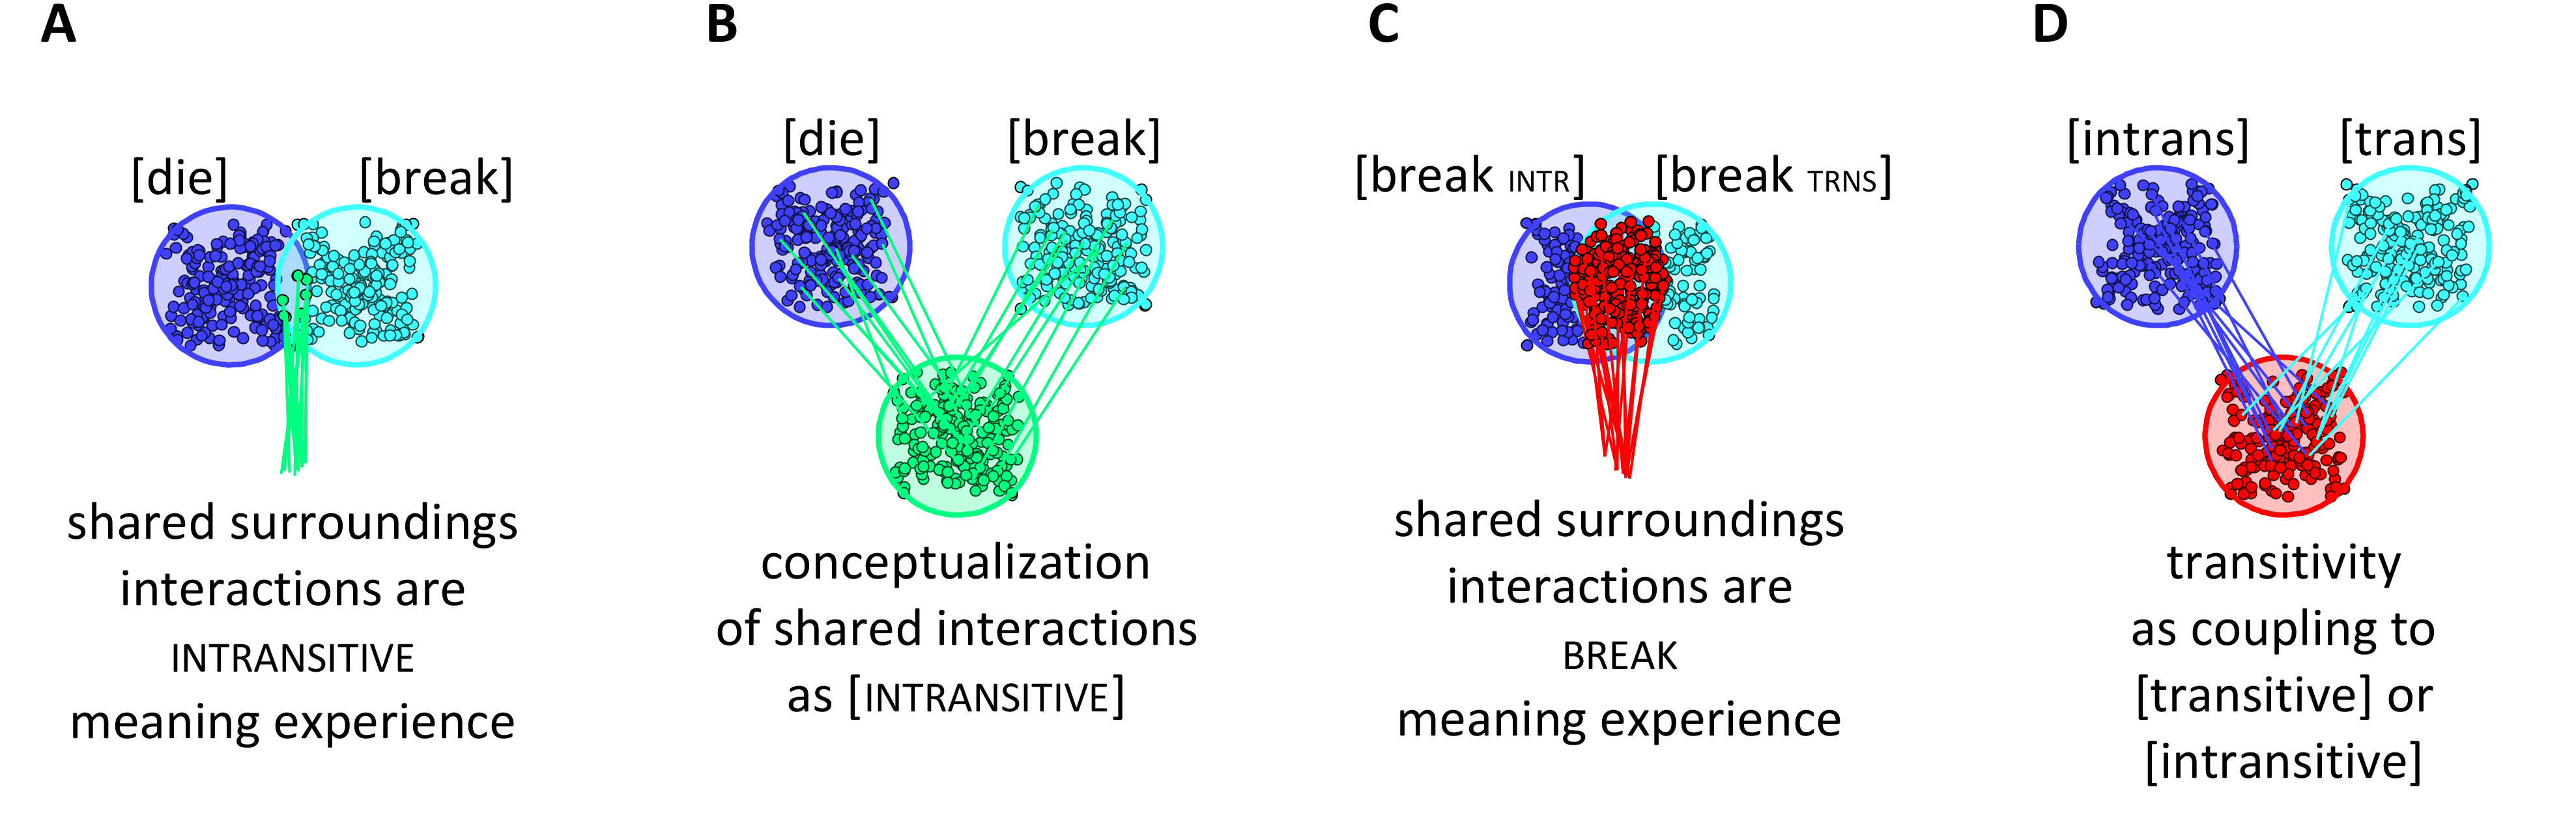
\includegraphics[width=\textwidth]{figures/Tilsen-img73.png}
\caption{\missingcaption}
\label{fig:4:23}
\end{figure}
 

  We can apply the same logic for reconceptualizing population overlap to (C) and (D): we interpret the intersection between [break\textsc{intr}] and [break\textsc{trans}] populations as a c-system [break] which interacts with [\textsc{intransitive}] or [\textsc{transitive}] c-systems. But these shifts in conceptualization—from population intersection to constructing a distinct system—are merely analytical changes on the macroscale. There is not necessarily a fundamental distinction between the relevant microstates. The macroscale decision to differentiate an existing system or construct a new class of system is simply a matter of analytical emphasis.

\subsection{Mechanisms of initial e-organization for basic word order}

Lets consider two possible views of how cs-systems are initially e-organized, with the aim of conceptualizing how basic word orders can differ across languages. Recall that in the canonical trajectory, the e-state stabilizes after a φ configuration stabilizes. We infer the temporal primacy of φ configurations from the existence of fixed word order languages, where there are large statistical nonuniformities in φ-e mappings. In contrast, in languages with relatively free word order, the distribution of φ-e mappings is relatively more uniform. What gives rise to these different distributions of φ-e mappings?

  To address this question, lets imagine idealized versions of fixed and free word order languages. To simplify the discussion, we consider only subjects and objects of transitive and intransitive verbs. For the idealized fixed word order language, we choose for convenience an English-like φ-e mapping: for transitive verbs, \{+N\}/\{-N\} occupy levels above/below \{V\}; for intransitive verbs the \{N\} argument always occupies a level above \{V\}. In the idealized free word order language, we assume statistical uniformity over all possible φ-e mappings. Hence we imagine the following distributions (a redder cell corresponds to a higher probability):

  
\begin{figure}
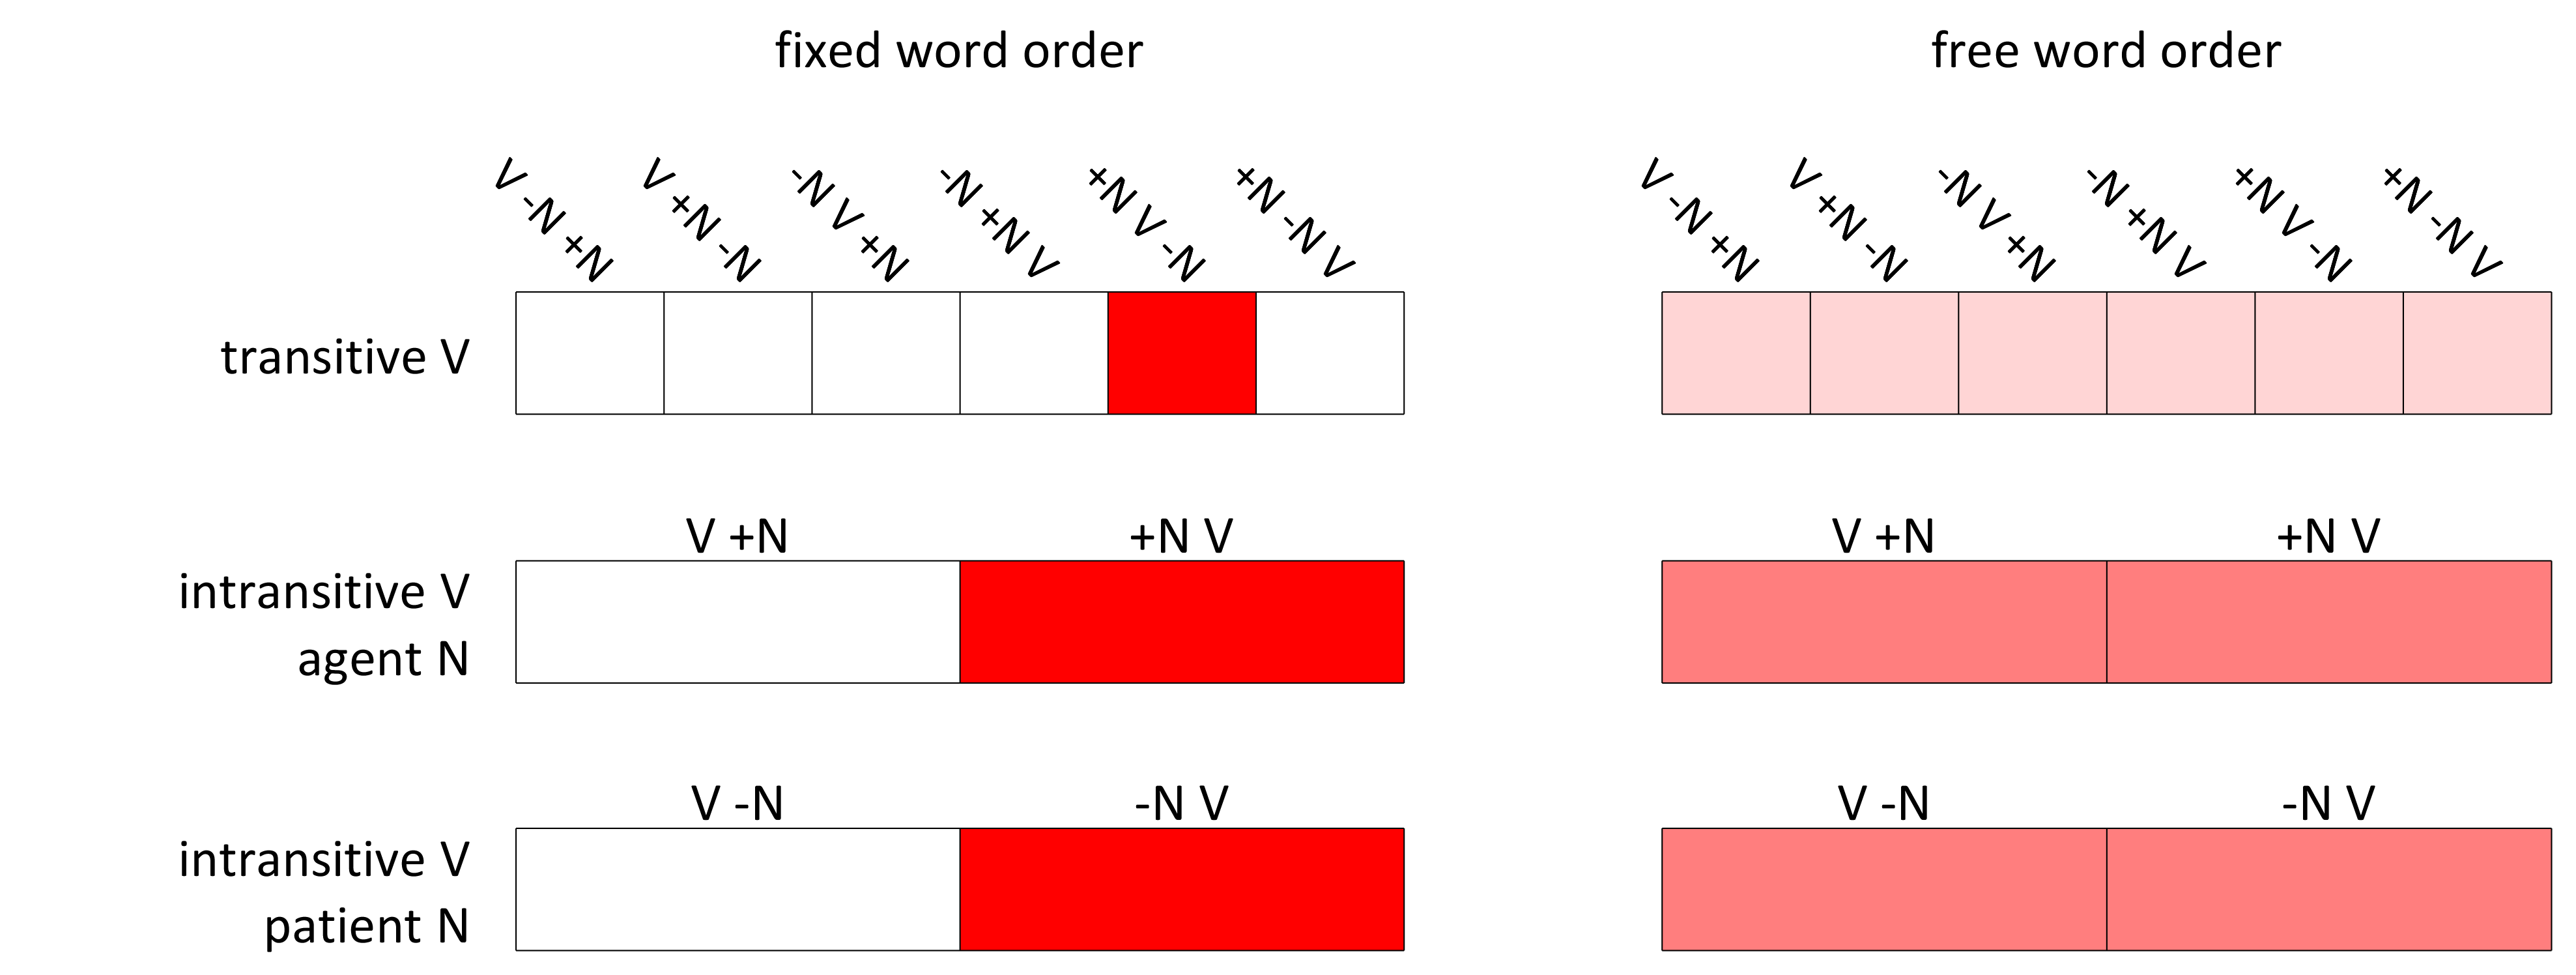
\includegraphics[width=\textwidth]{figures/Tilsen-img74.png}
\caption{\missingcaption}
\label{fig:4:24}
\end{figure}
 

  How could such drastic differences in distributions of φ{}-e mappings arise from a common mechanism? Lets imagine that excitation of a \{V\} system gives rise to “unoccupied” e-levels for argument \{N\} systems. Note that this contradicts our earlier conclusion that each s-system, through its interactions with other s-systems, creates its own e-level, and hence the notion of an unoccupied level (excepting ground- and selection- levels) is not sensible. For the moment we ignore this contradiction.

  Furthermore, lets imagine that for transitive verbs, \{+N\} and \{-N\} compete to occupy the highest unoccupied level. For SVO fixed order, \{V\} gives rise to one level above and below itself, the relevant order is obtained when \{+N\} is e-organized before \{-N\}, i.e. when organization of \{+N\} has precedence over \{-N\}. This \{+N\} > \{-N\} scheme, when crossed with the three possible ways that \{V\} can create two levels, generates the three most common basic word orders, SOV, SVO, and VSO, as shown below. The relatively rare VOS, OSV, and OVS orders follow from a \{-N\} > \{+N\} scheme, where \{-N\} is e-organized before \{+N\}:

  
\begin{figure}
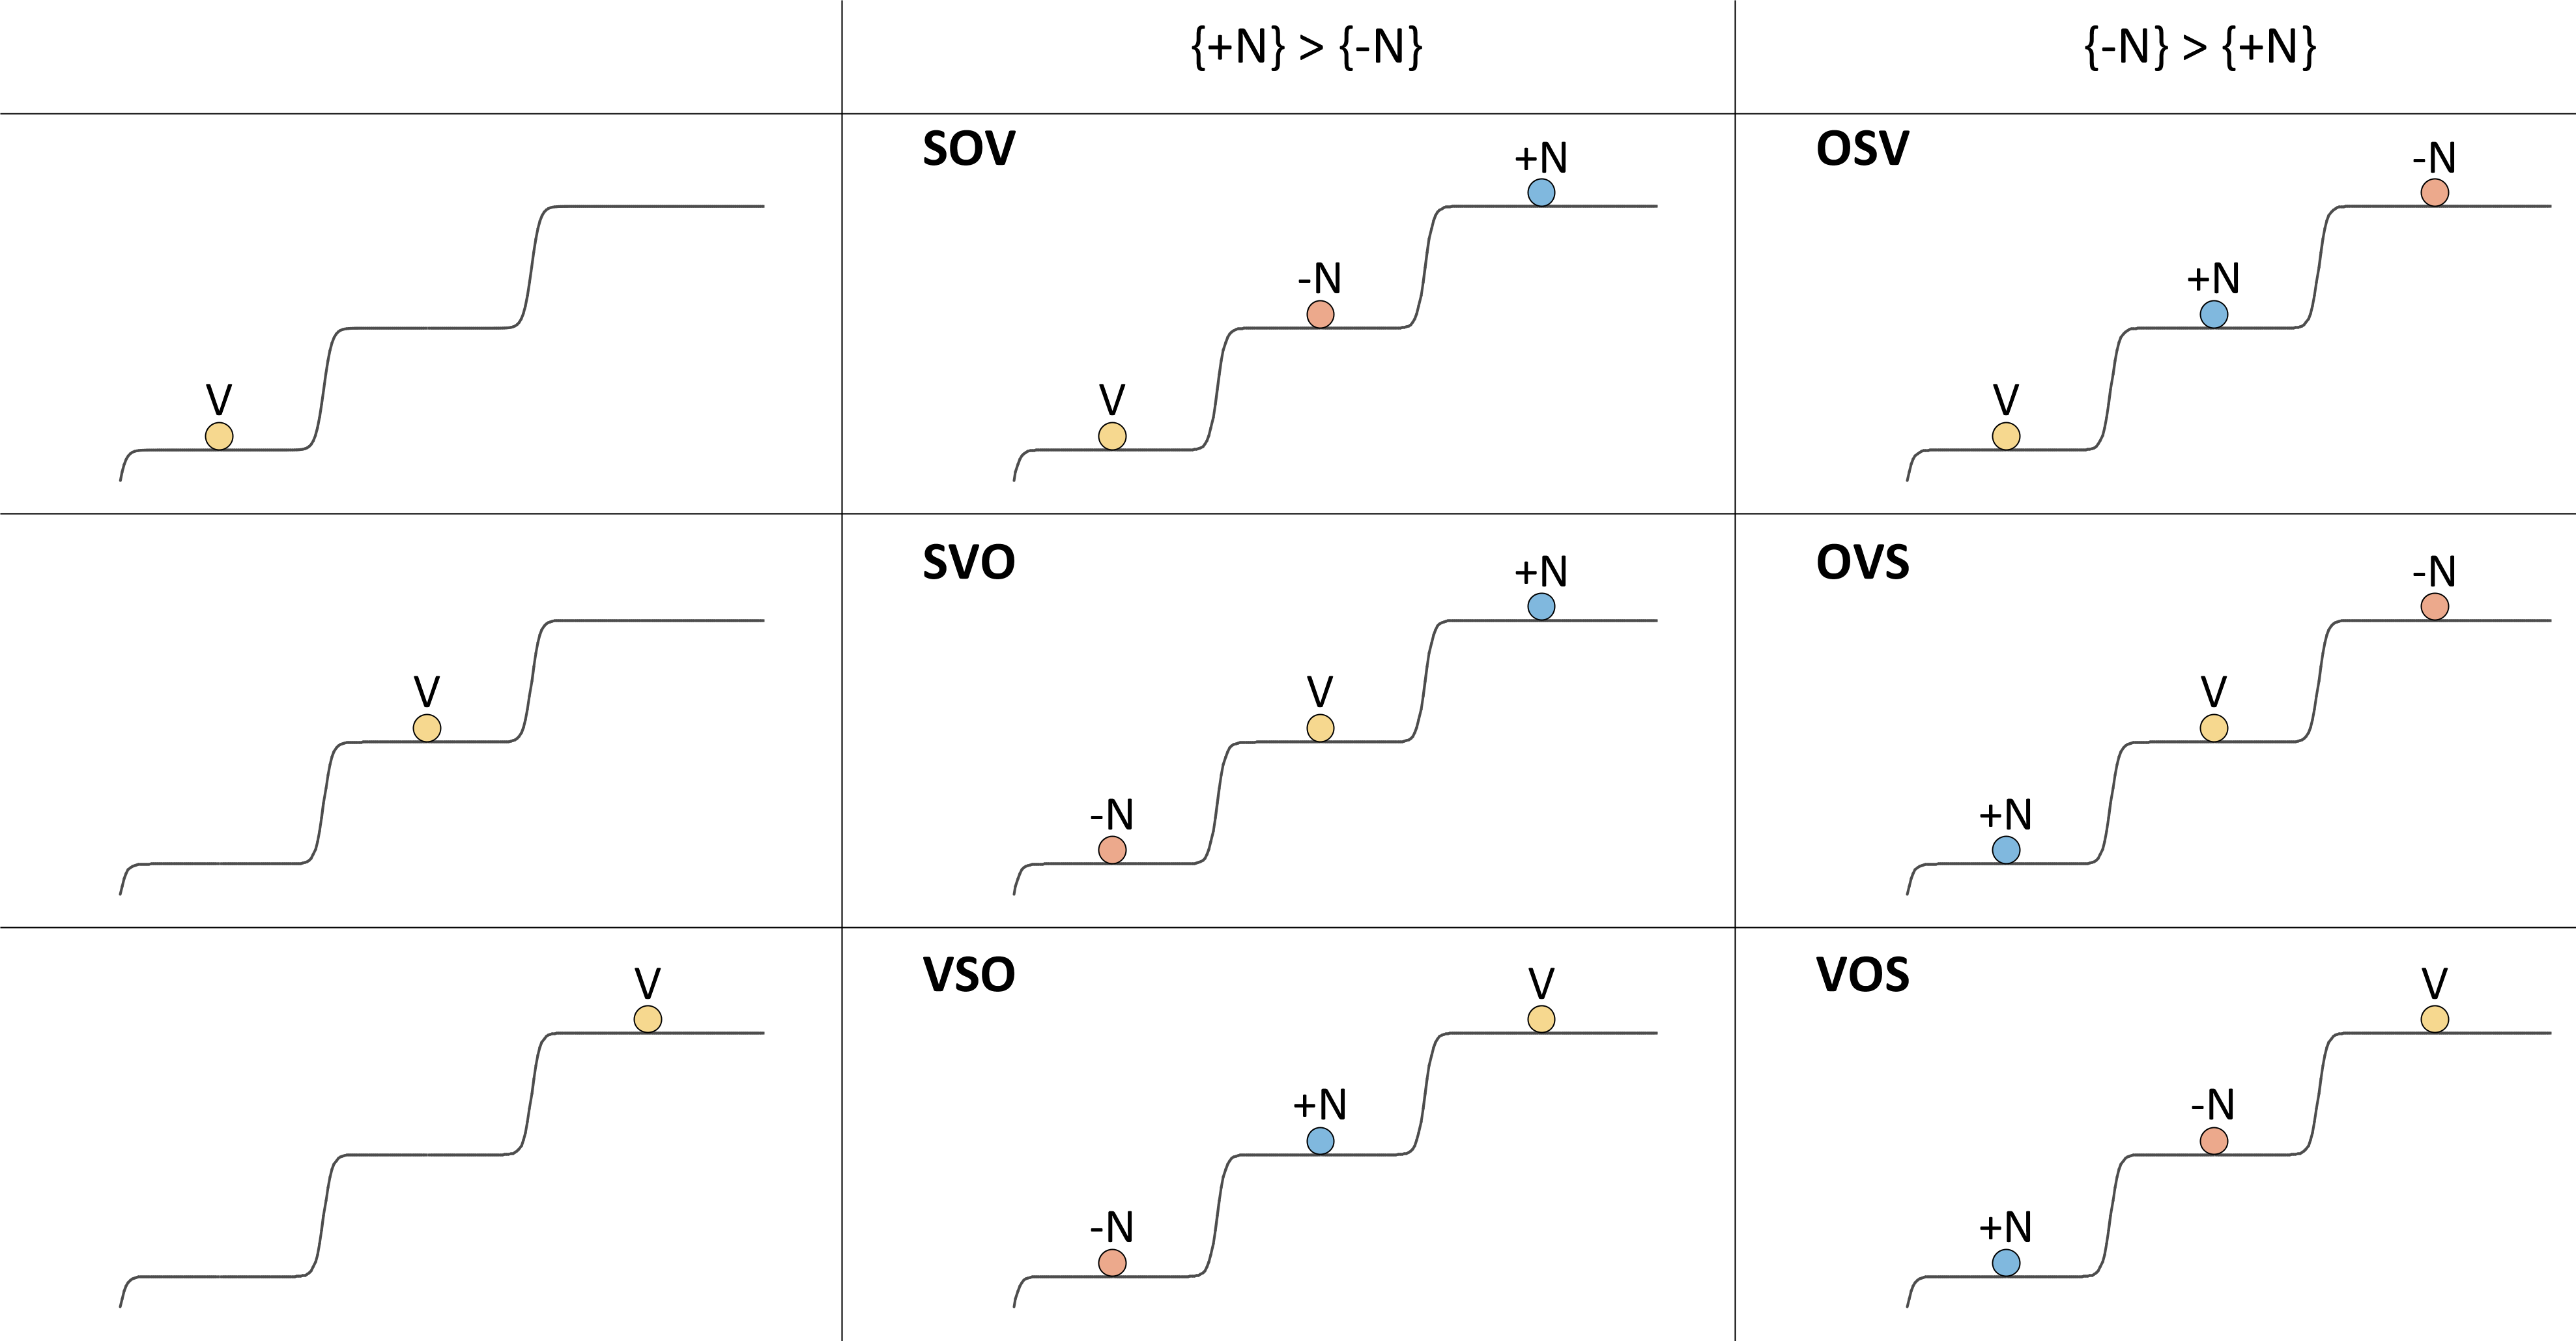
\includegraphics[width=\textwidth]{figures/Tilsen-img75.png}
\caption{\missingcaption}
\label{fig:4:25}
\end{figure}
 

  To apply the above conception to an idealized free order language we simply abandon the notion of priority between \{+N\} and \{-N\} and allow for the assignment of \{N\} systems to e-levels to be random. (There are a number of specific variations on this random assignment scheme which generate free order, such as creating multiple levels above and below \{V\} or assigning \{V\} to an unoccupied level as well.)

  One thing that is appealing about the level-occupation metaphor is that it readily describes a correlation between \{V\} valence and e-organization. The excitation of a \{V\} system seems to organize the excitation of \{N\} systems in a manner that depends on the c-system(s) which resonate with \{V\}. The level-occupation metaphor suggests an analogy to atomic systems and energy levels of electrons. The composition of an atomic nucleus determines available orbitals for electrons, with each orbital being associated with a specific energy. Although our cs-systems are macroscopic, their behavior is quantal in a phenomenological sense. Indeed, if lexical s-systems such as \{N\}, \{V\}, \{Adj\}, and \{Adv\} never occupy the same e-level, they effectively obey an exclusion principle. In contrast, grammatical s-systems such as \{D\}, \{\textsc{tense}\}, \{\textsc{person}\}, etc. can jointly occupy e-levels with a lexical system. Although construing \{V\} as a nucleus is tempting, it conflicts with the conceptual mapping between orbital radius and excitation level. The analogy thus suggests a representation in which cs-systems occupy a discrete set of orbits as below.

  
\begin{figure}
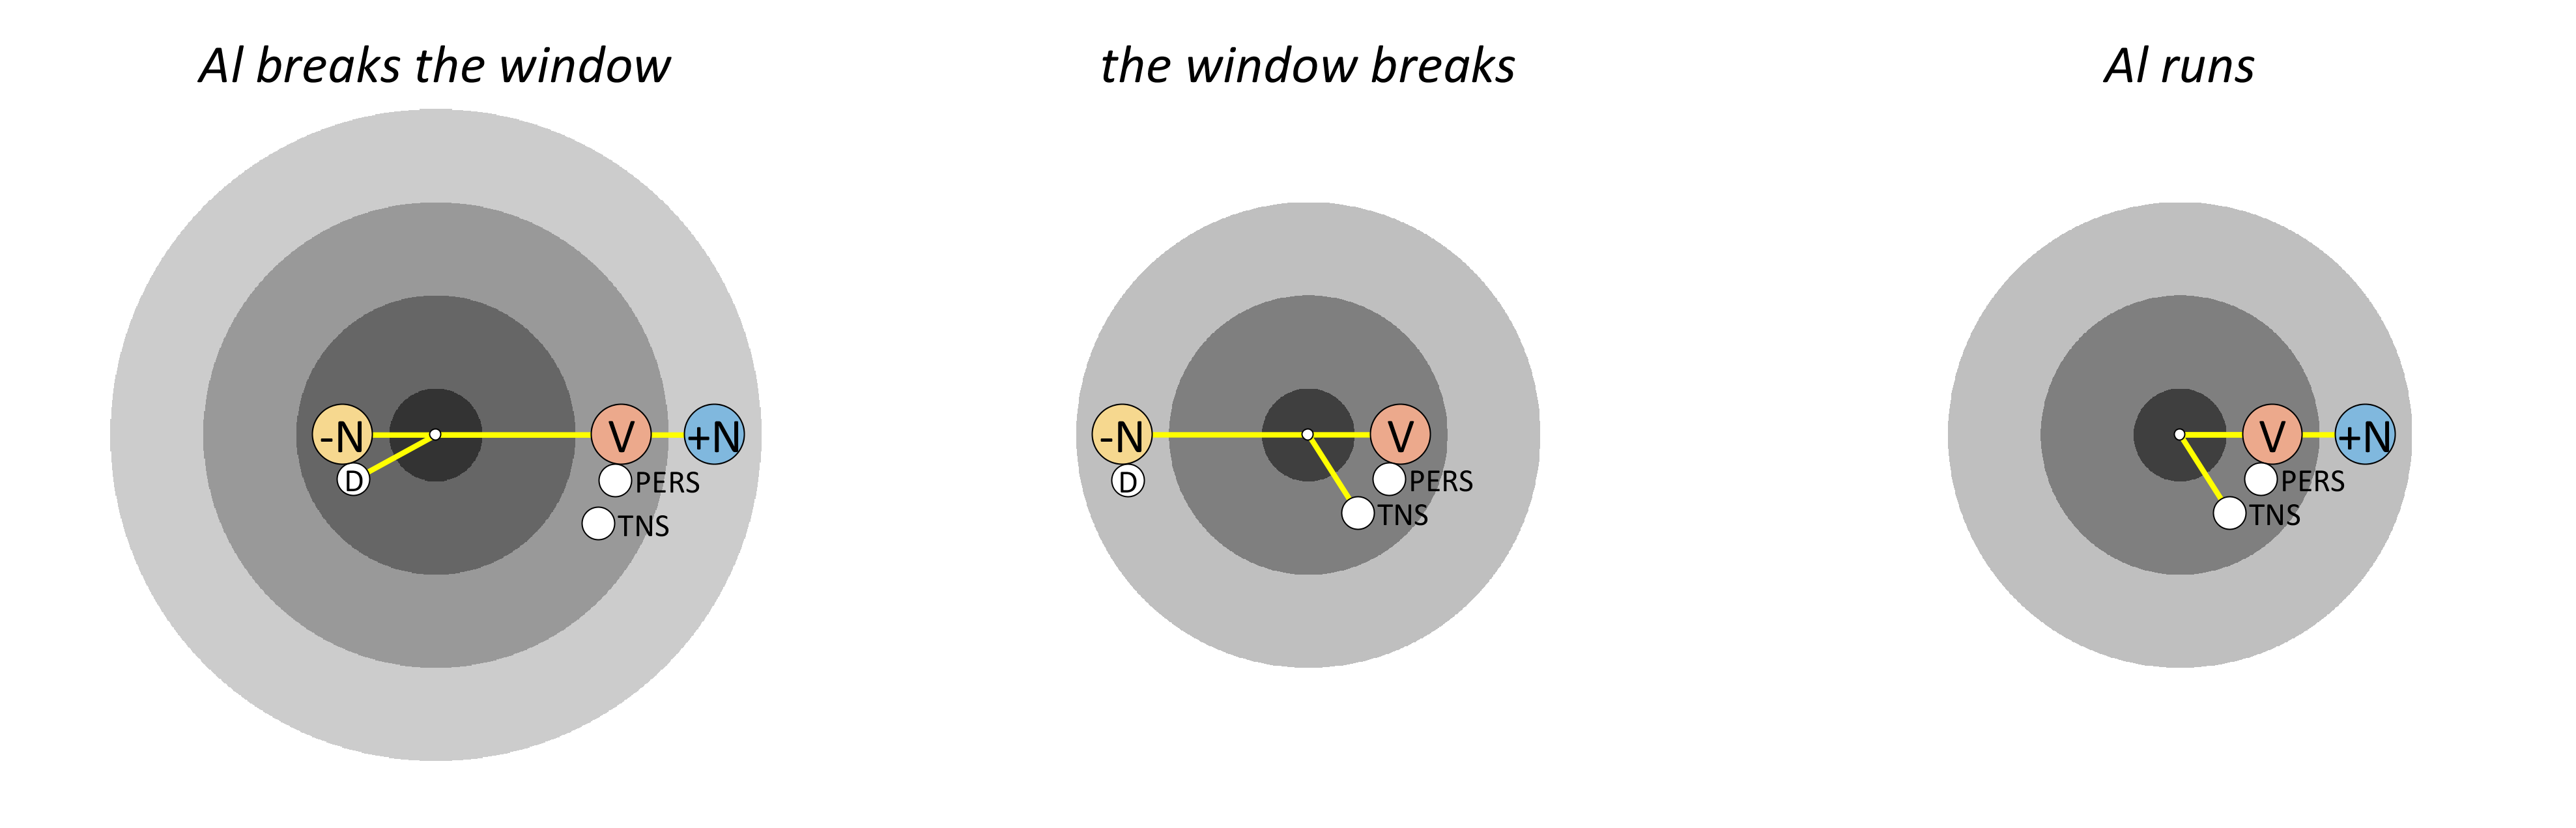
\includegraphics[width=\textwidth]{figures/Tilsen-img76.png}
\caption{\missingcaption}
\label{fig:4:26}
\end{figure}
 

  Note that orbital schemas are problematic because they can be mistaken to imply distances between systems. For example, in \textit{Al breaks the window}, the orbital schema implies that [Al]\{+N\} is closer to [breaks]\{V\} than to [window]\{-N\}; this is merely an artefact of mapping two spatially unrelated dimensions, e and φ, onto polar coordinates, which wrongly reifies the systems as objects in space, rather than states.

  A deeper problem with the word ordering mechanism described above is its reliance on the notion of an unoccupied e-level. In our original construction of the e-potential, the quantal nature of e-levels was understood to emerge from local interactions between systems. The notion that \{V\} organizes levels independently of \{N\} systems contradicts this interpretation. To be careful, we must be remember to view the quantal e-potential as an emergent consequence of s-system interactions, and \textit{not} as a reified spatial structure which exists independently from \textit{objects} which occupy those locations—we should not allow the object metaphor to reinvade our conceptual model. Thus a conceptual model that does not require unoccupied e-levels is preferable.

  Another issue with the above mechanism is that it is suitable for only the \textit{idealized} fixed and free word order patterns. In an empirical sense, there are no languages which conform to the idealized patterns: free word order languages tend to depart substantially from uniformity, and fixed word order languages never have maximally ordered distributions, allowing for constructions such as topicalization, passivization, etc. Thus there is a continuum between fixed and free order. 

  How should we conceptualize the mechanism which is responsible for this continuum? In developing the canonical production trajectory, we imagined that (i) cs-systems are activated, (ii) c-systems compete (because of interference) for strong cs-resonances, and (iii) the outcome of the competition is that some cs-systems are excited (above-ground), while others are active but unexcited (ground level) or perhaps even deactivated. In that picture, we made no assumptions regarding the relative \textit{e} values of c-systems or s-systems before a stable configuration emerges. Prior to stabilization, we expect short term averages of phase velocities $\theta ′$ and \textit{e} values of s-systems to be highly variable. We can imagine the pre-stable phase as a \textit{disordered regime} (a “high temperature” regime), with high-amplitude fluctuations in system states. The emergence of a stable configuration requires a transition to an \textit{ordered regime} (a low temperature regime) in which fluctuations in \textit{e} and φ have diminished. For an s-system, the sources of the “fluctuations” in the disordered regime are its interactions with many c-systems, which in general will have different \textit{f}, θ, and \textit{e} from each other. When multiple c-systems begin to resonate with one s-system, these differences can pull the θ and \textit{f} of the s-system in different directions. This interference potentially destabilizes cs-resonances. Furthermore, because s-systems are strongly coupled to each other, the fluctuations that an s-system experiences induce fluctuations in the forces which the system exerts on other s-systems, possibly destabilizing those systems.

  How does a set of cs-resonances ever stabilize, given the high degree of variability in the pre-stable phase? Presumably, some c-systems are more highly excited than others, or become so during the pre-stable phase, due to their surroundings interactions. If these particular systems become sufficiently excited relative to their competitors, then their resonances with s-systems can be strong enough to stabilize, and an ordered organization of cs-systems can emerge. Moreover, as shown below, the specific pattern of relative excitation that emerges could depend on random fluctuations in the pre-stable phase: the relative e-pattern that obtains as the system begins to cool becomes more and more likely to persist as fluctuations diminish.

   
\begin{figure}
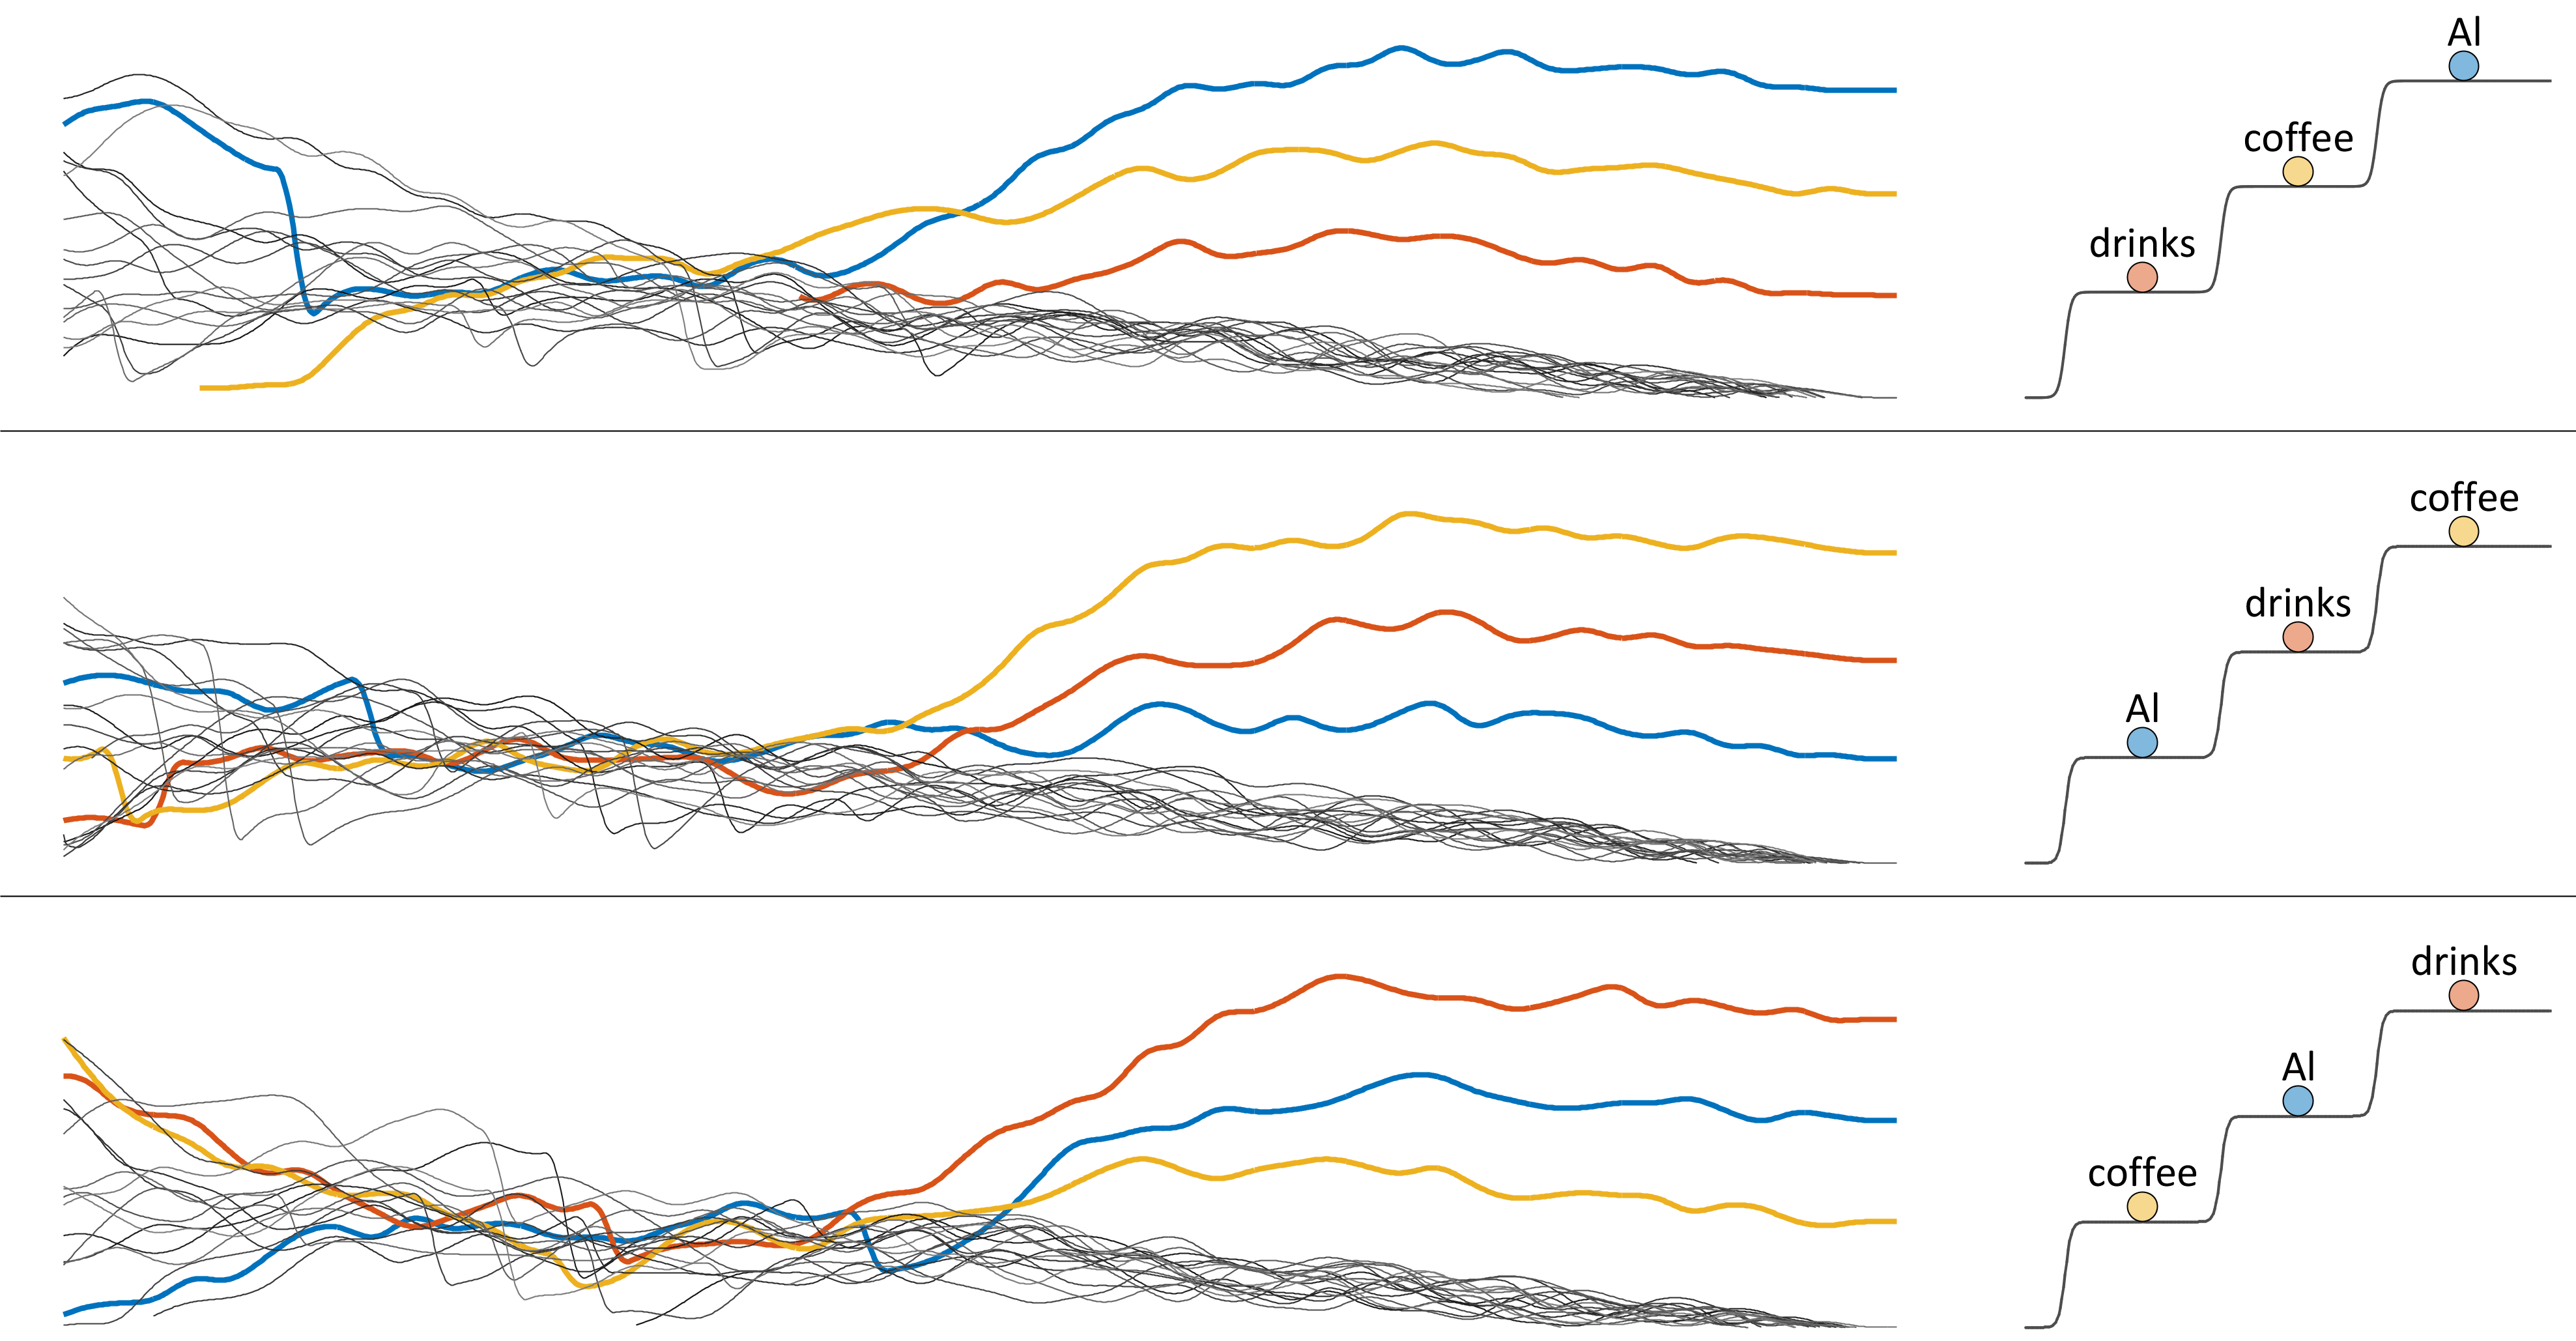
\includegraphics[width=\textwidth]{figures/Tilsen-img77.png}
\caption{\missingcaption}
\label{fig:4:27}
\end{figure}
 

  This elaborated picture presents a highly chaotic evolution of s-systems in the pre-stable phase of a production trajectory: new cs-resonances may appear and vanish, corresponding to the emergence and decay of collective oscillations, i.e. the activation and deactivation of systems. The interactions between these oscillations and the surroundings can have complex effects. The stable initial e configuration that emerges as the system transitions to the ordered regime can depend sensitively on system states during the disordered regime. An analogy to a liquid-glass transition may be useful here: stable configurations have a semi-crystalline organization, because they are asymmetric in relative \textit{e} space; the cooling process is rapid; stable configurations emerge when the amplitudes of fluctuations become small in comparison to the strengths of the stabilizing forces associated with cs-resonances and s-system coupling.

  It may be possible to develop a more detailed framework for understanding the disordered and ordered regimes as high temperature and low temperature respectively. First, we invoke the thermodynamic conception of temperature, T = dE/dS, as the amount of thermal energy required to increase the entropy of a system. We associate energy E with \textit{e} value and entropy S with the logarithm of the number of accessible states, or of the volume of state space which is accessible. Note that when in the pre-stable phase, the volume of \textit{e} and $\theta ′$ space which a system visits in some short time interval is larger than the volume visited in the stable phase, and hence the entropy is larger. We then reason that if we could inject energy into a system, i.e. increase its \textit{e} value, the effect of that increase on S is smaller in the high T regime than in the low T regime. In other words, more energy needs to be injected in the high T regime than in the low T regime, in order to produce the same increase in S (i.e. volume of state space visited by the system).

  Why does the system begin in a high temperature phase and then cool? Perhaps there is no way to activate only a small set of c-systems. The surroundings forces which initially activate c-systems may always influence many c-systems. But when many c-systems interact with the same s-system, interference (because of differences in \textit{f}, θ, and \textit{e} of the c-systems) prevents any one of the cs-resonances from being stable. A relaxation/cooling process is necessary to allow some small set of cs-systems to stabilize into an ordered state. Would an organization mechanism that avoids this messy process be preferable? Perhaps not, because a system that somehow created order instantaneously would have no way of adapting to variation in influences from its surroundings: the pre-stable phase is what makes it possible for surroundings forces to exert a bias on the relative excitation of systems, and without this phase, relational meaning experiences would be highly stereotyped.

Statistical departures from the uniformity of idealized free word order distribution can be understood in this framework. Under the assumptions of random uniform initial conditions and symmetric interaction forces, we expect all ordered e configurations to emerge from the cooling process with equal likelihood, resulting in the idealized free order pattern. But if initial conditions are not random for any reason (e.g. because sensory systems induce semantically correlated differences in c-system initial excitation), we expect departures from uniformity.

  Even larger departures from maximal non-uniformity, as in idealized fixed order, can also be interpreted from this perspective. Fixed order arises when s-system interaction forces are strongly asymmetric. If those forces are strong enough to outweigh the influences of fluctuations in the pre-stable phase, state trajectories will more frequently evolve to a fixed order that depends on the particular pattern of asymmetry. These interaction asymmetries must be learned, since fixed orders differ across languages. Since no language exhibits perfect non-uniformity, we can infer that the learned asymmetries, no matter how strong, are never strong enough to outweigh the strongest surroundings influences.

  To account for the rarity of basic word orders where \{-N\} is initially organized with a higher \textit{e} value than \{+N\}, we conjecture that our perception of events (i.e. surroundings forces) imposes statistical biases on the relative timing of system activation or on \textit{e} values. These could be such that \{+N\} agent/experiencer resonances tend to arise earlier and with higher \textit{e} than \{-N\} patient/theme resonances. This could be a consequence of how humans attend to the world, and our impression that actions proceed causes, which relates to the apparent directionality of time. Furthermore, +φ coupling is more stable than -φ coupling. This could have many consequences for the timecourse of cs-resonance stabilization. For example, greater stability entails greater resistance to perturbations. During the high temperature phase, the +φ coupling between \{+N\} and \{V\} could stabilize earlier and be less susceptible to perturbation than the -φ coupling between \{-N\} and \{V\}. Assuming that φ stability results in increased \textit{e}, the difference in coupling stability predicts the \{+N\} > \{-N\} bias.

\subsection{Influence of the pre-stable phase on initial organization}

The highly ordered, stable φ/e configuration that emerges as an initial configuration in a canonical trajectory evolves from a disordered, pre-stable phase. In the o/el conceptual model, the specific configuration that stabilizes can depend only on the system state and surroundings. The initial states of the system and surroundings in the pre-stable phase determine the subsequent trajectory toward some stable configuration. In other words, a stabilized configuration in a production trajectory is never truly random: it is always determined by previous states. Any apparent randomness is simply a consequence of our lack of knowledge of the system and surroundings.

  One major gap in our model is a detailed conception of the evolution equations of the system in the pre-stable phase, in which we do not imagine a quantal e-potential to exert stabilizing forces. In particular, we have a great deal of uncertainty regarding how \textit{e} variables of systems change over time in this regime. This contrasts with the stable regime, in which we assume that we can usefully approximate changes in relative \textit{e} with discrete operations on relative \textit{e}. Recall that previously we proposed two regimes for the excitation operator, a stabilizing regime Ê\textsuperscript{st} which maps stable e-states to themselves, and a reorganizing regime associated with a canonical reorganization Ê\textsuperscript{cr}. The canonical reorganization demotes selected systems to the first excitation level and promotes other systems. 

  We also referred earlier to an initial organization operator Ê\textsuperscript{io}. The initial organization operator can be interpreted as an analytic tool for thinking about the outcome of the cooling mechanism which governs the transition from a disordered, non-quantal e-state to an ordered, quantal e-state. The tool Ê\textsuperscript{io} has the property that it maps a non-quantal e-state—which we have very little certainty about—to a quantal e configuration. We think of Ê\textsuperscript{io} as a deterministic mapping, and construct hypotheses about how pre-stable states are mapped to stable e configurations. One clear difference between Ê\textsuperscript{io} and Ê\textsuperscript{cr}/Ê\textsuperscript{st} is that initial organization can depend on φ-states, whereas canonical reorganization and stabilization do not. 

  Cases where identical or similar φ configurations are associated with different e-organizations may thus be helpful for drawing inferences regarding how Ê\textsuperscript{io} depends on e-states. The logic here is that if φ-states of two different initial e configurations are the same or similar, then differences in pre-stable e-states must be responsible for the difference in initial e configuration. 

  Topicalization and inverted pseudo-cleft constructions are examples of such cases. Consider the patterns in (B) and (C): [coffee]\{N\} is initially organized at selection level, rather than below \{V\} as is in the basic order. We suspect that these patterns arise when [coffee]\{N\} has abnormally high excitation in the pre-stable phase. This could be due to surroundings forces, such as a context in which [coffee] contrasts with a previously excited concept (e.g. \textit{Al doesnt drink tea…coffee, he drinks}). Importantly, the deviation cannot be readily understood as a consequence of differences in φ-organization, since the {\textbar}Al drinks coffee{\textbar} configuration is present in all three examples. (Note that our analysis of [\textsc{focus}] as +φ coupled to \{N\} applies here; furthermore, in the inverted pseudo-cleft the copula [\textsc{be}] is hypothesized to +φ couple with two arguments, [coffee]\{-N\} and [what]\{-N\}, and so [\textsc{be}] must resonate with an s-system other than \{V\}. We use \{\textit{v}\} for this copular s-system.)

  
\begin{figure}
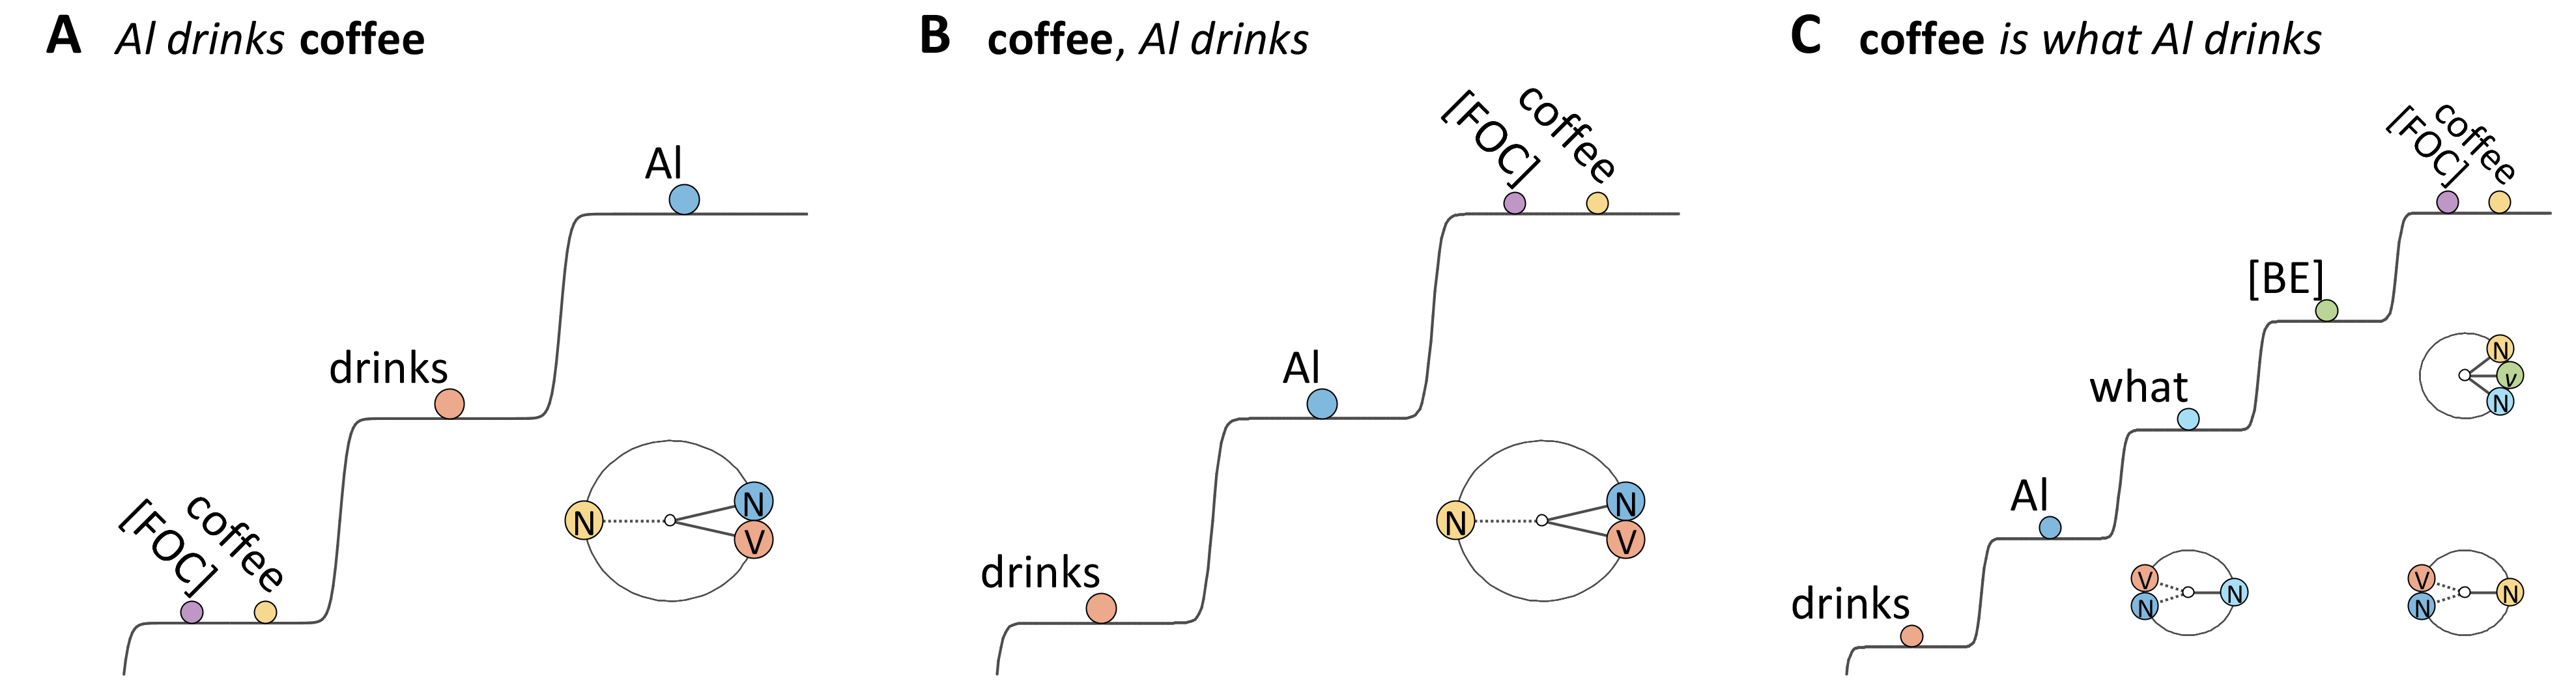
\includegraphics[width=\textwidth]{figures/Tilsen-img78.png}
\caption{\missingcaption}
\label{fig:4:28}
\end{figure}
 

  Example (A) shows that [\textsc{focus}] does not necessarily result a promotion of \{-N\} to selection level. Similarly, in the pseudocleft in (D), even though \{-N\} is coupled with [\textsc{focus}], it is not promoted relative to other systems. Furthermore, even when [coffee]\{-N\} is promoted, the syntactic manifestation of basic word order can be preserved with pronominal forms, as in the cleft construction in (E). Somewhat archaic variants with non-canonical word order as in (F) can occur in some dialects. These examples force us to conclude that augmented excitation in the pre-stable epoch can create biases on Ê\textsuperscript{io}, but is not sufficient to determine its output. 

  
\begin{figure}
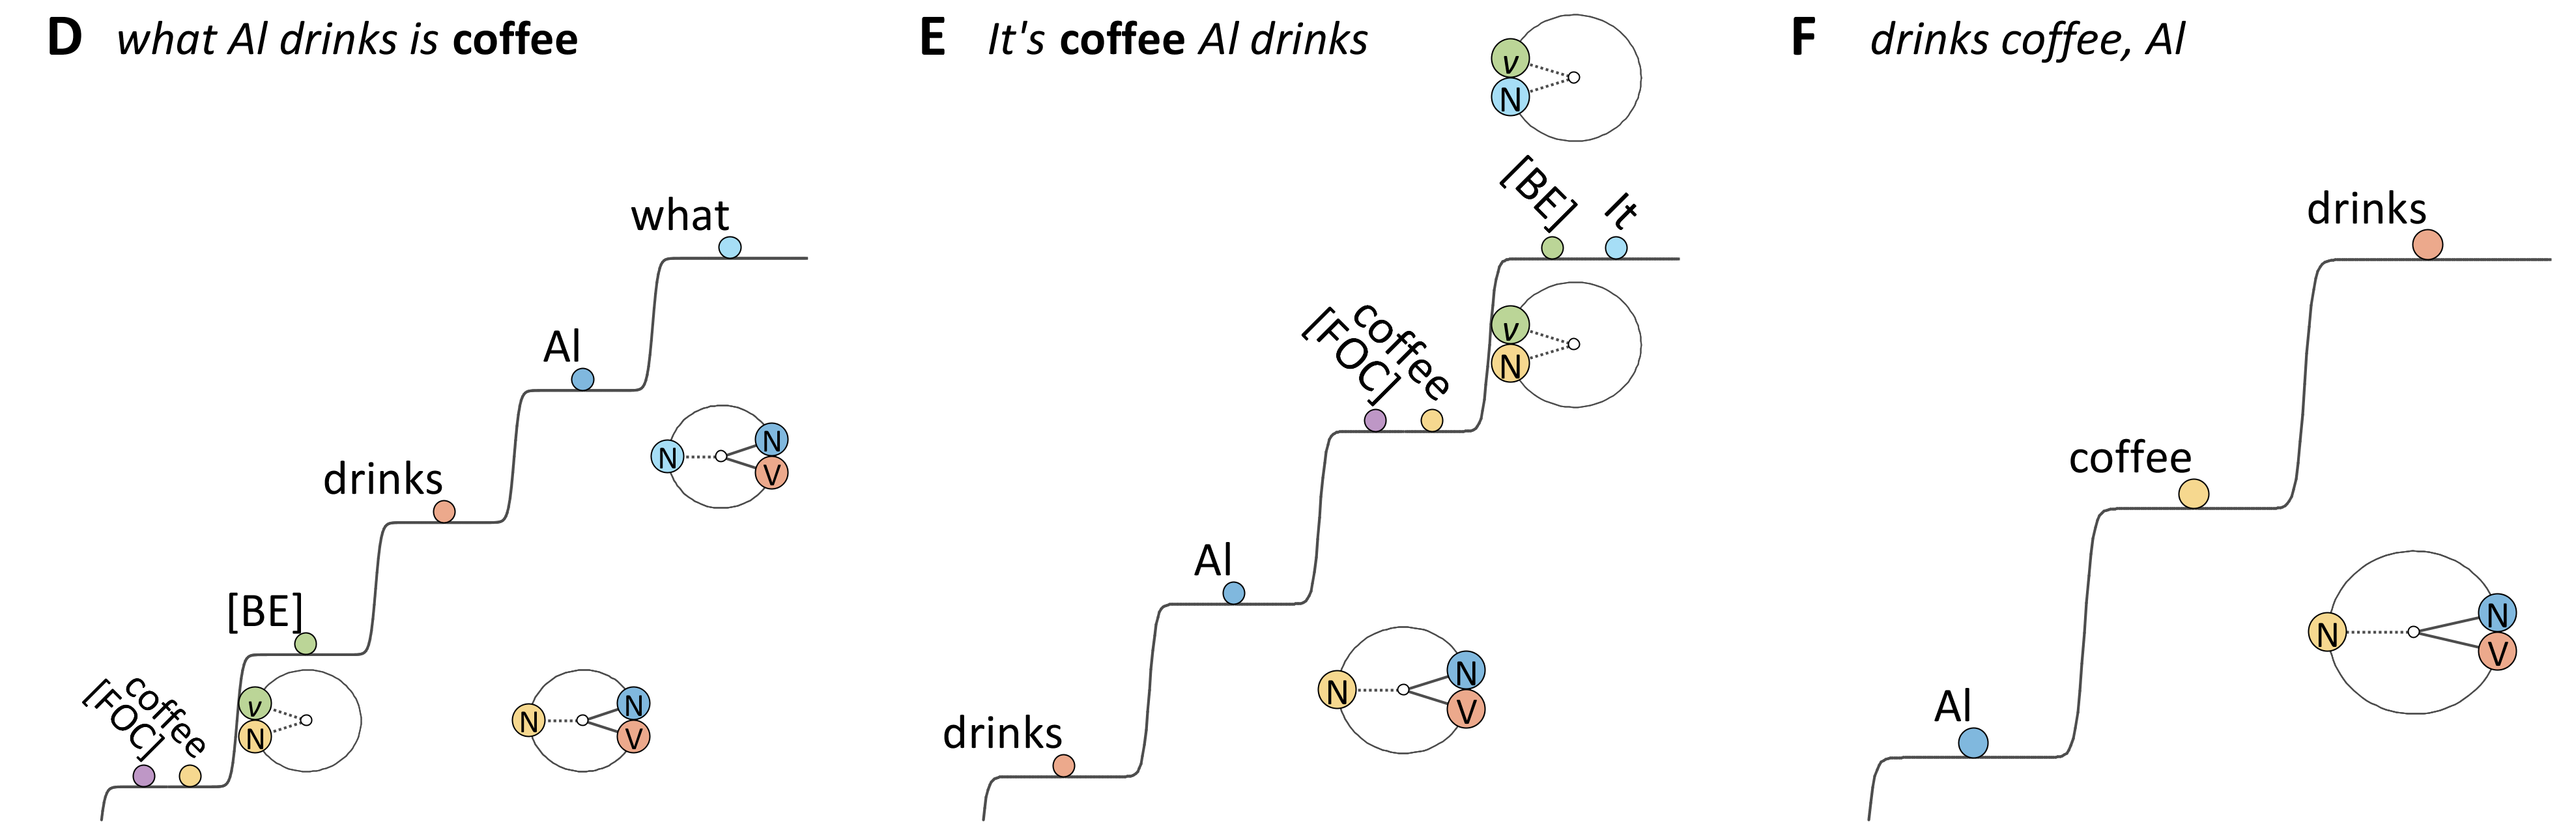
\includegraphics[width=\textwidth]{figures/Tilsen-img79.png}
\caption{\missingcaption}
\label{fig:4:29}
\end{figure}
 

  Another example of similar φ configurations with different e-organizations involves ditransitive constructions. A recipient \{N\} can be e-organized above or below the theme/patient one, as shown in examples (A)-(C) below. The recipient system [Bo]\{N\} in all cases is in a -φ configuration with [give]\{V\}, regardless of the whether a prepositional \{P\} system is excited. In the configurations with a preposition, the configuration arises more indirectly, because \{-N\} and \{P\} are -φ coupled, and \{P\} and \{V\} are +φ coupled. This is consistent with the observation that indirect objects can sometimes be omitted, c.f. \textit{Al gave coffee} vs. *\textit{Al gave Bo}. The analysis also gels with our assumption that \{P\} systems typically -φ couple to an argument and +φ couple to a modificand, thereby establishing a relational meaning experience between the argument and modificand. Here the \{P\} system relates the action [give]\{V\} and the recipient [Bo]\{N\}. In other types of ditransitives, such as \textit{Al put coffee on the table}, \{P\} relates an action and location argument. The inference we draw here is that some aspect of the pre-stable state, other than φ configuration, is likely responsible for the variation. The pre-stable relative \textit{e} values of the recipient and patient systems is a plausible source of such variation in initial organization.

  
\begin{figure}
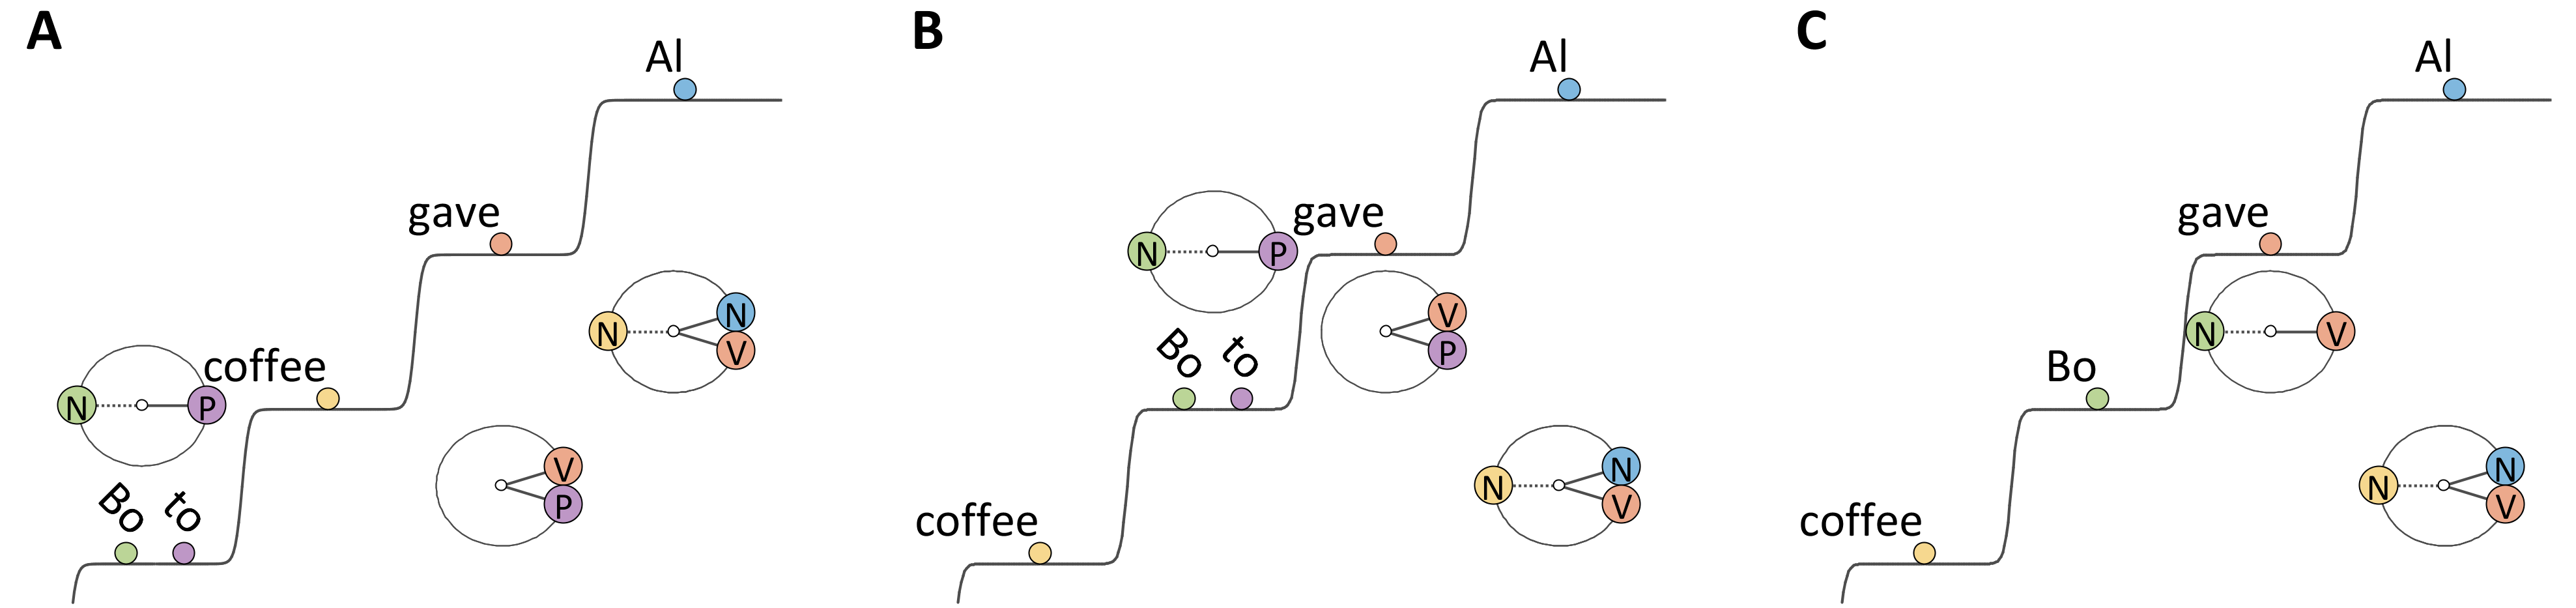
\includegraphics[width=\textwidth]{figures/Tilsen-img80.png}
\caption{\missingcaption}
\label{fig:4:30}
\end{figure}
 

  More examples of variation in e organization that is not driven by φ configuration are found in passive constructions. The φ-invariance principle dictates that the patient/theme argument of the passive has a -φ relation with \{V\} and that the agentive argument has a +φ relation. (Note that the adjunct [by]\{P\} is -φ coupled to [Al]\{+N\}, and hence cannot be +φ coupled to [drink]\{V\}. The [by]\{P\} system thus differs from typical \{P\} systems, which accords with conventional analyses that treat passive by-phrases as special). The passive constructions in (A)-(C) have the same (or similar) φ configurations as the active construction; hence we suspect that differences in relative \textit{e} value prior to stabilization may influence whether the output of Ê\textsuperscript{io} corresponds to a passive or active pattern.

  
\begin{figure}
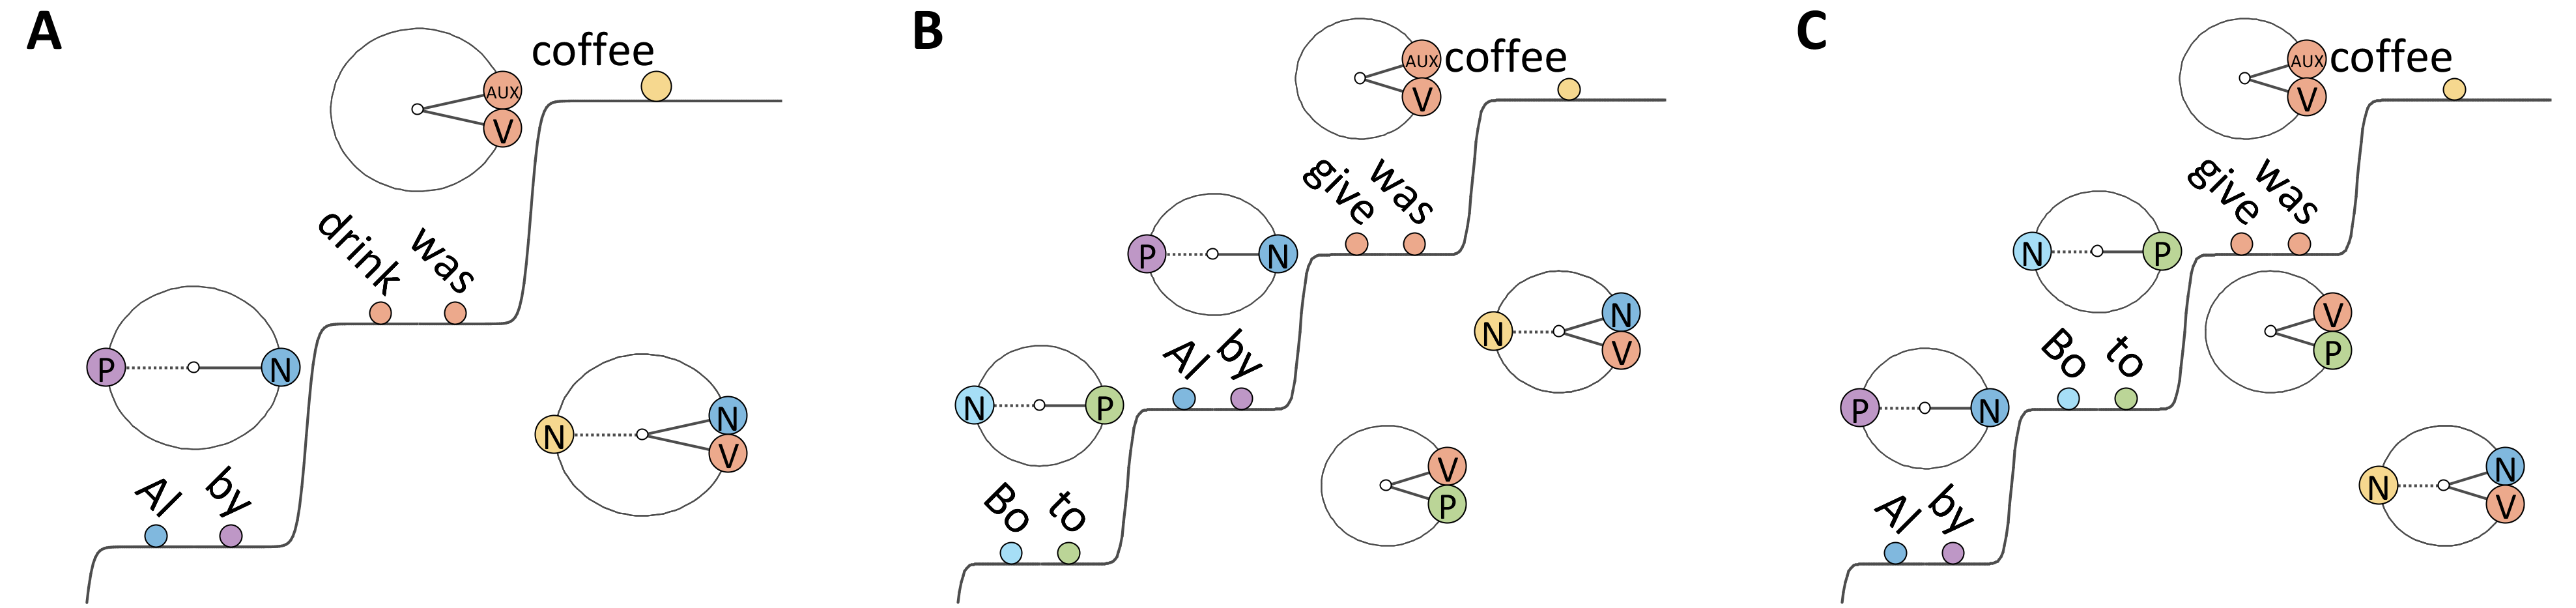
\includegraphics[width=\textwidth]{figures/Tilsen-img81.png}
\caption{\missingcaption}
\label{fig:4:31}
\end{figure}
 

  From the ditransitive and passive examples above, we infer that initial e-organization is not entirely determined by φ configuration. Moreover, we can perhaps draw some inferences about the state space regions from which the evolution of such trajectories would be more or less likely. A reasonable conjecture is that relative excitation of arguments in ditransitives and passivized ditransitives could be influenced by relative excitation prior to stabilization.

  Some further examples of e-organization not conditioned on φ configuration involve nominalized verbs with arguments. As shown below, we analyze nominalized verbs as co-selection of \{V\} with a nominalizing system [\textsc{nom}]\{N\}, e.g. [drink]\{V\}-[\textsc{nom}]\{\textsc{N}\}. Some alternative analyses—which may not be distinct on the microscale—would be to posit the differentiation [drink,\textsc{verbal}] vs. [drink,\textsc{nominal}], or to couple [drink] and \{N\}. Notably, all of the examples below evoke the same relational meaning configuration between [Al], [drink], and [coffee].

  
\begin{figure}
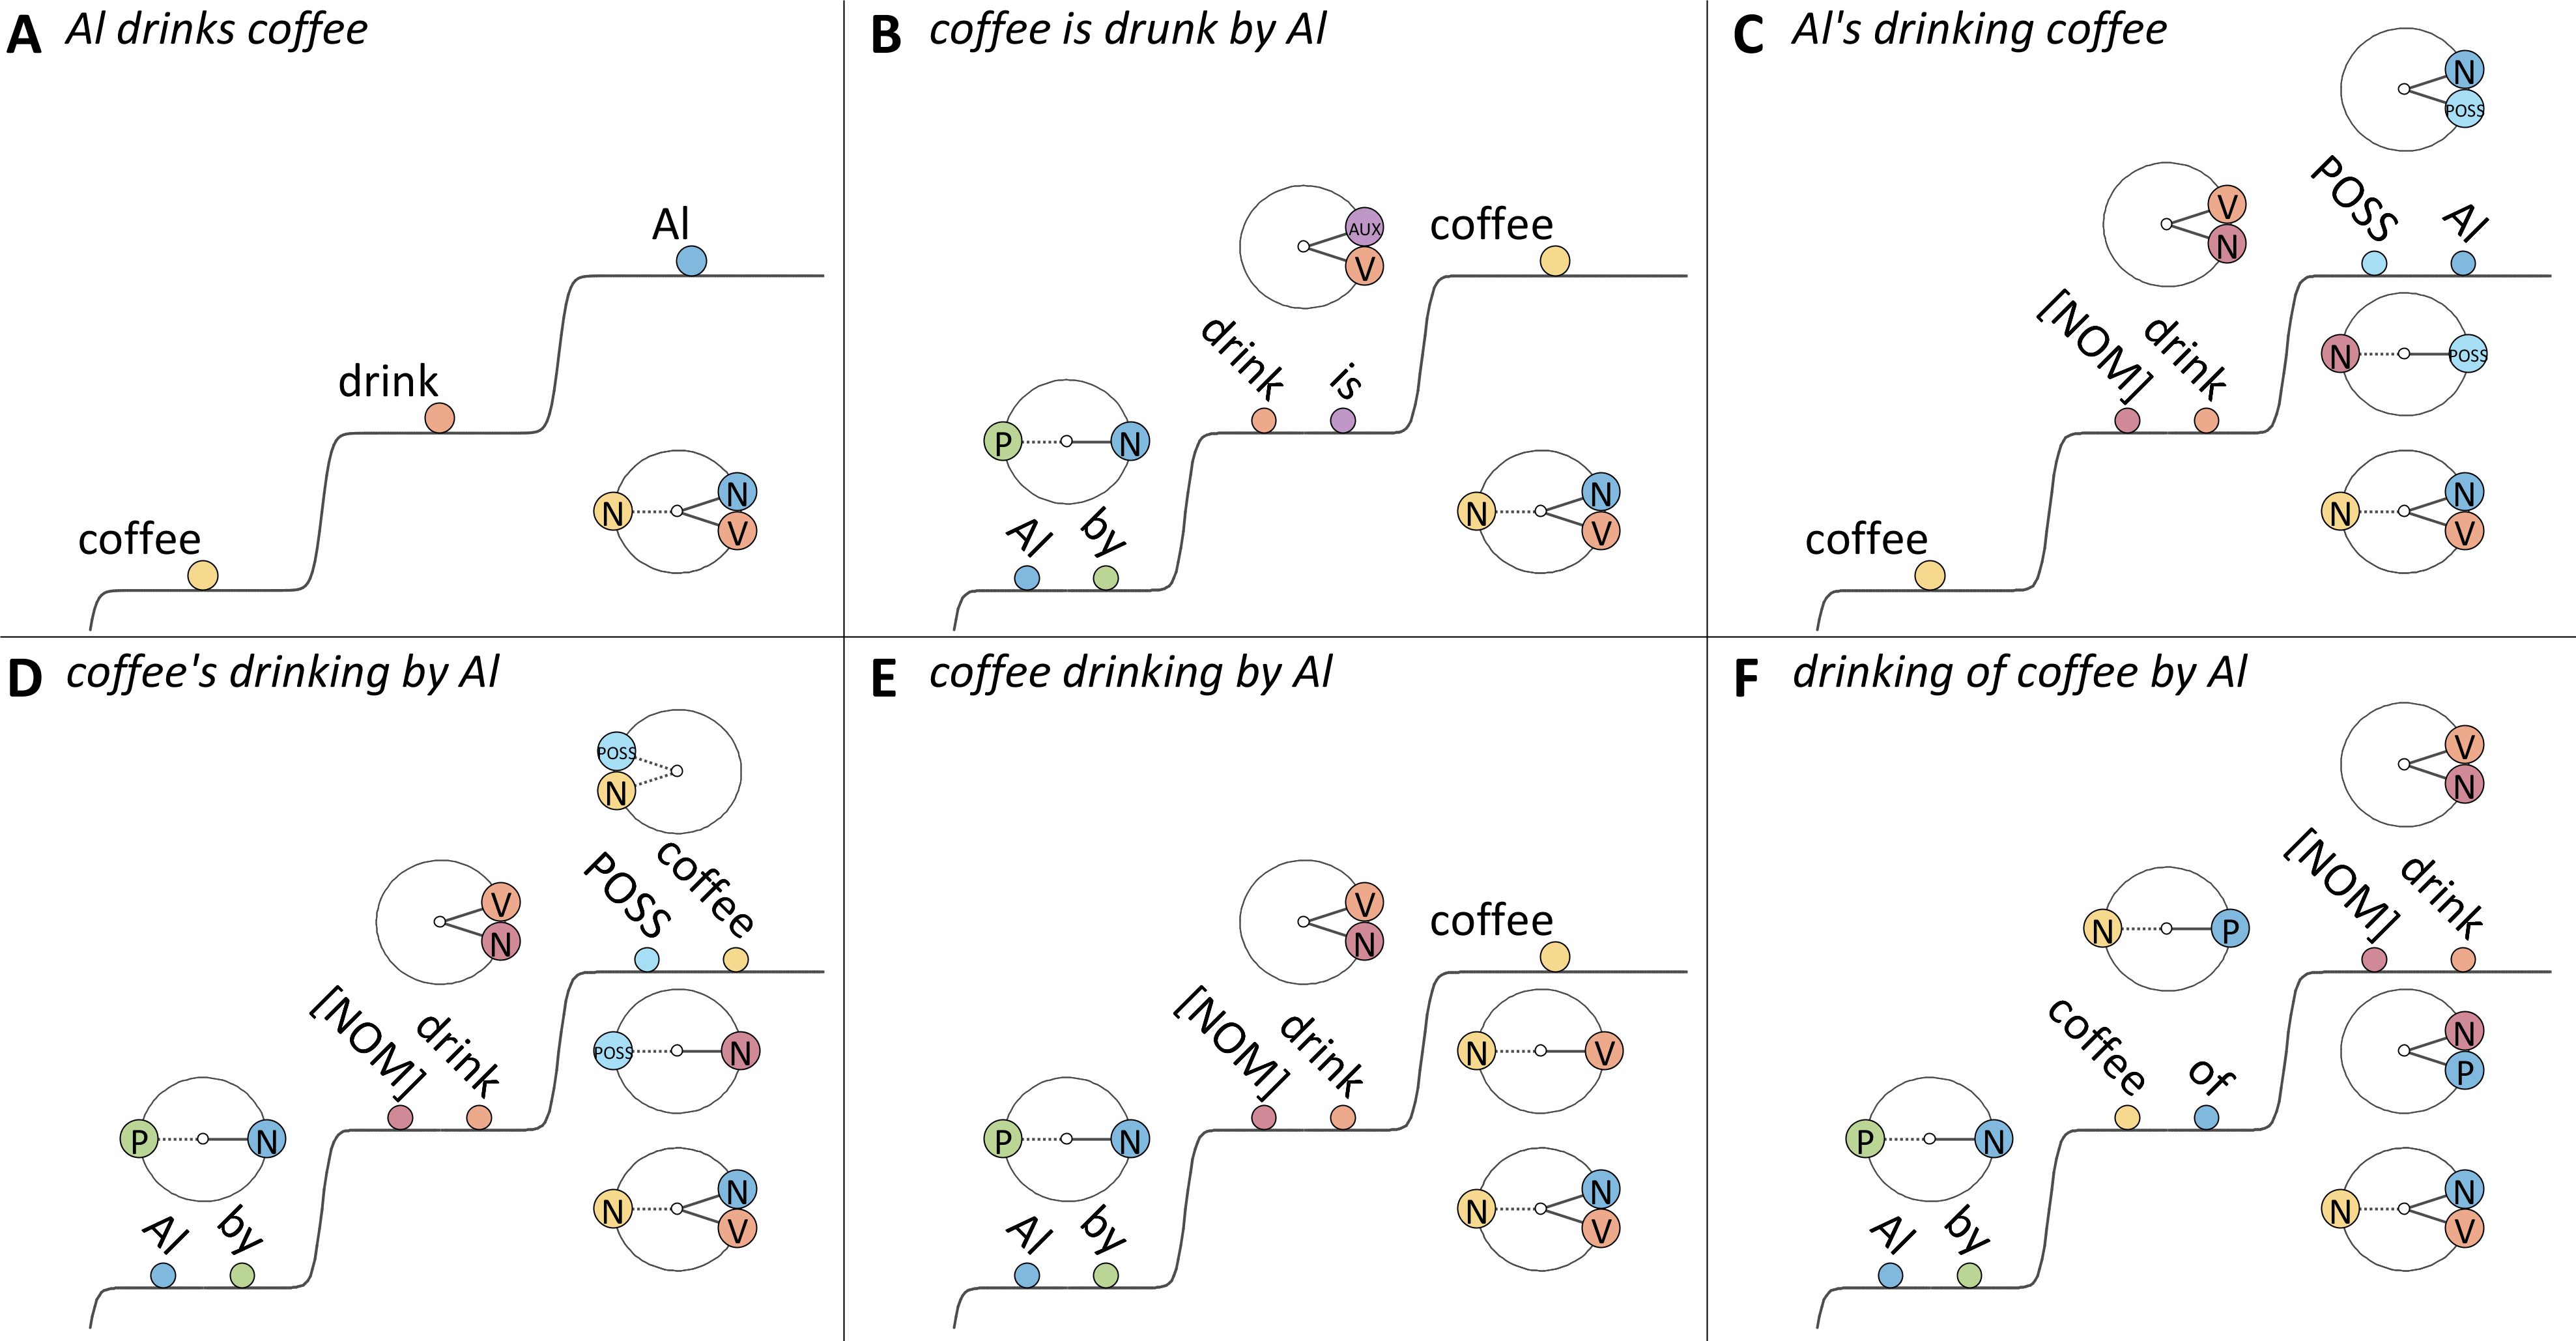
\includegraphics[width=\textwidth]{figures/Tilsen-img82.png}
\caption{\missingcaption}
\label{fig:4:32}
\end{figure}
 

  Currently we can only speculate on how such diversity in e-organization can arise from similar φ configurations. The nominalization of verbal meaning experiences may be understood as consequence of surroundings biases which deemphasize the {\textbar}Al drinks coffee{\textbar} configuration relative to some other configuration. In general, to conceptualize variation in the output of Ê\textsuperscript{io} we imagine that there are distinct regions of state space from which pre-stable trajectories evolve to a stable organization. Numerous outcomes of this process are possible—topicalizations, clefts, passives, nominalizations, etc. There appear to be no fixed order languages which lack at least some of these constructions. Augmented excitation of specific systems in the pre-stable phase is one plausible source of such variation, but there are likely other sources that remain to be discovered. Another important consideration is that the time course of activation relative to initial organization is probably important. Careful experimentation in sentence production tasks may be able to shed light on such influences.

\subsection{Context dependence of optionality/obligatoriness}

Conventional approaches to phrase structure often distinguish between arguments, which are purportedly “obligatory”, and adjuncts, which are purportedly “optional”. In the examples below, [Al]\{N\} and [coffee]\{N\} are considered arguments, while [cold]\{ADJ\}, [quickly]\{ADV\}, [brewed]\{V\}, and [yesterday]\{ADV\} are considered adjuncts. The valence of adjunct φ-coupling depends on the semantic relation of the adjunct to the relevant lexical system that it modifies. \{V\} adjuncts in a theme/patient relation with an \{N\} are -φ coupled to another system, as is the case for \{N\}[coffee] and \{V\}[brewed]; \{P\} adjuncts are +φ coupled to a modificand and -φ coupled to a complement \{N\}. All other adjuncts are +φ coupled to a lexical system.

  
\begin{figure}
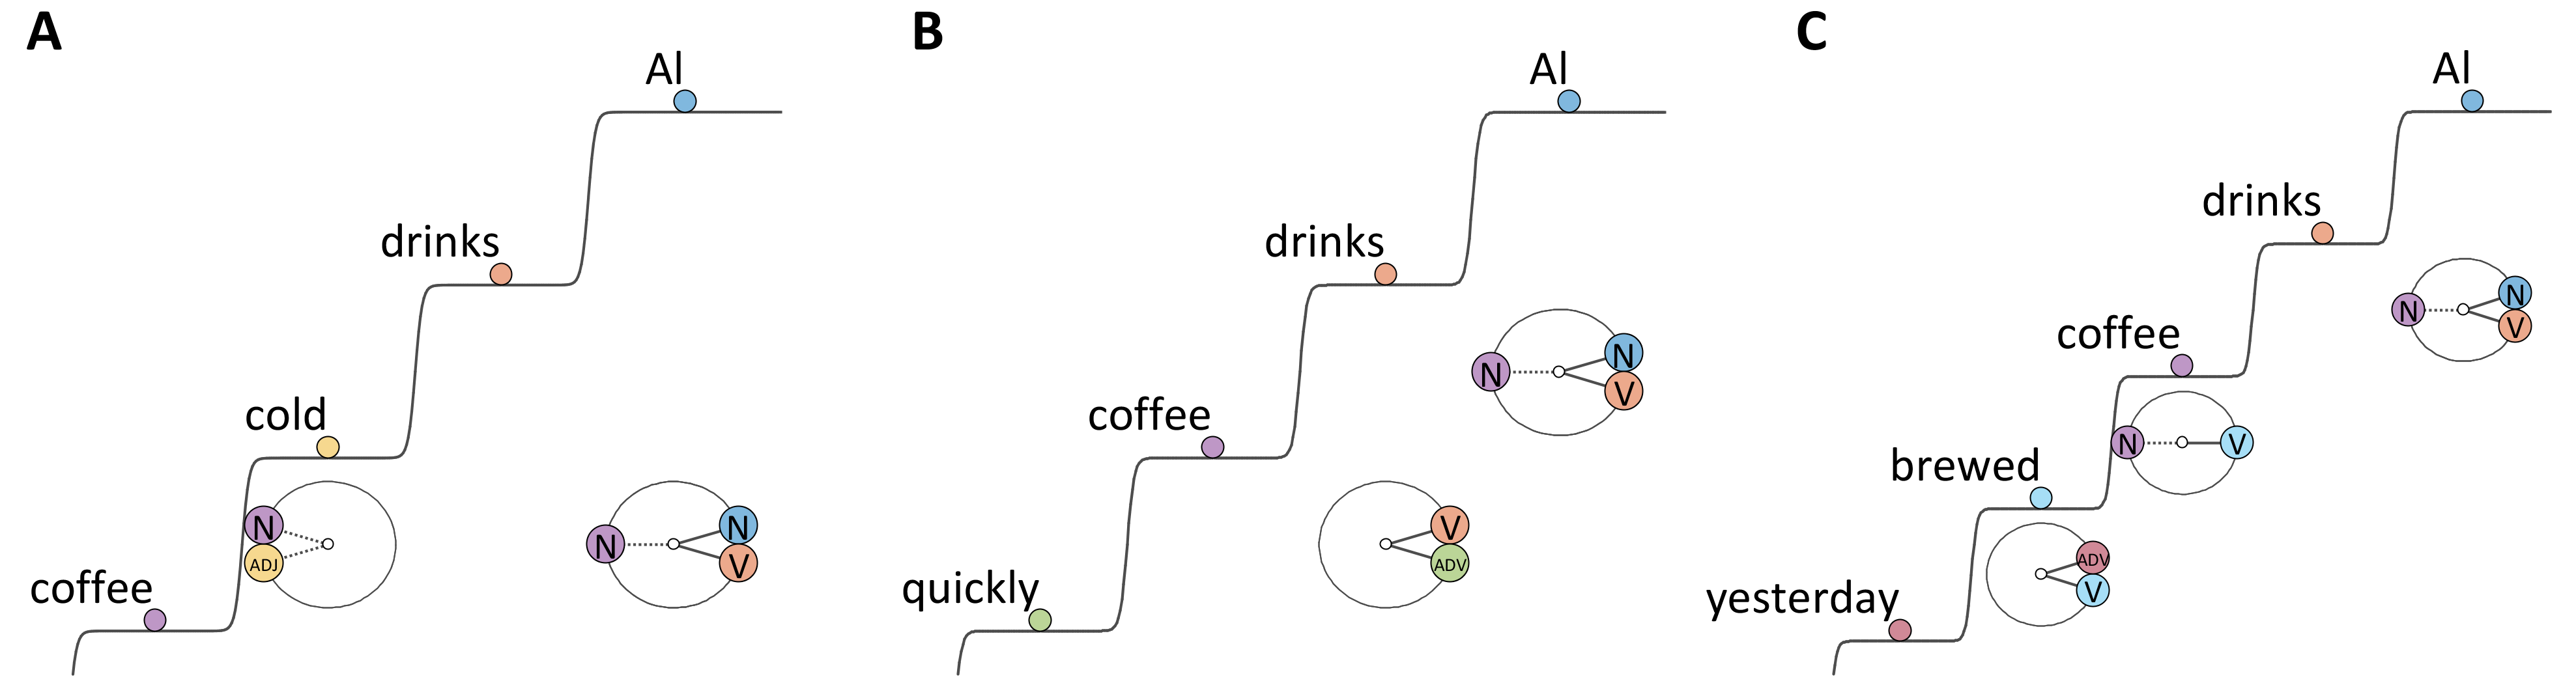
\includegraphics[width=\textwidth]{figures/Tilsen-img83.png}
\caption{\missingcaption}
\label{fig:4:33}
\end{figure}
 

  Whereas \{ADJ\} and \{ADV\} only φ-couple to one other s-system, prepositional and verbal adjuncts \{P\} and \{V\} can φ-couple to two systems, as in (A)-(C) below. Hence [with]\{P\} in \textit{Al drinks coffee with sugar} is +φ coupled to [coffee]\{N\} and -φ coupled to [sugar]\{N\}. This is consistent with an intuition that the intended meaning experience of \textit{coffee with sugar} is a relation between the coffee and the sugar. Likewise, in \textit{Al drinks coffee with Bo}, [with]\{P\} is +φ coupled to [drinks]\{V\} and -φ coupled to [Bo]\{N\}, because the intended experience involves a relation between the act of drinking and the presence of Bo, as opposed to a relation between coffee and Bo.

  
\begin{figure}
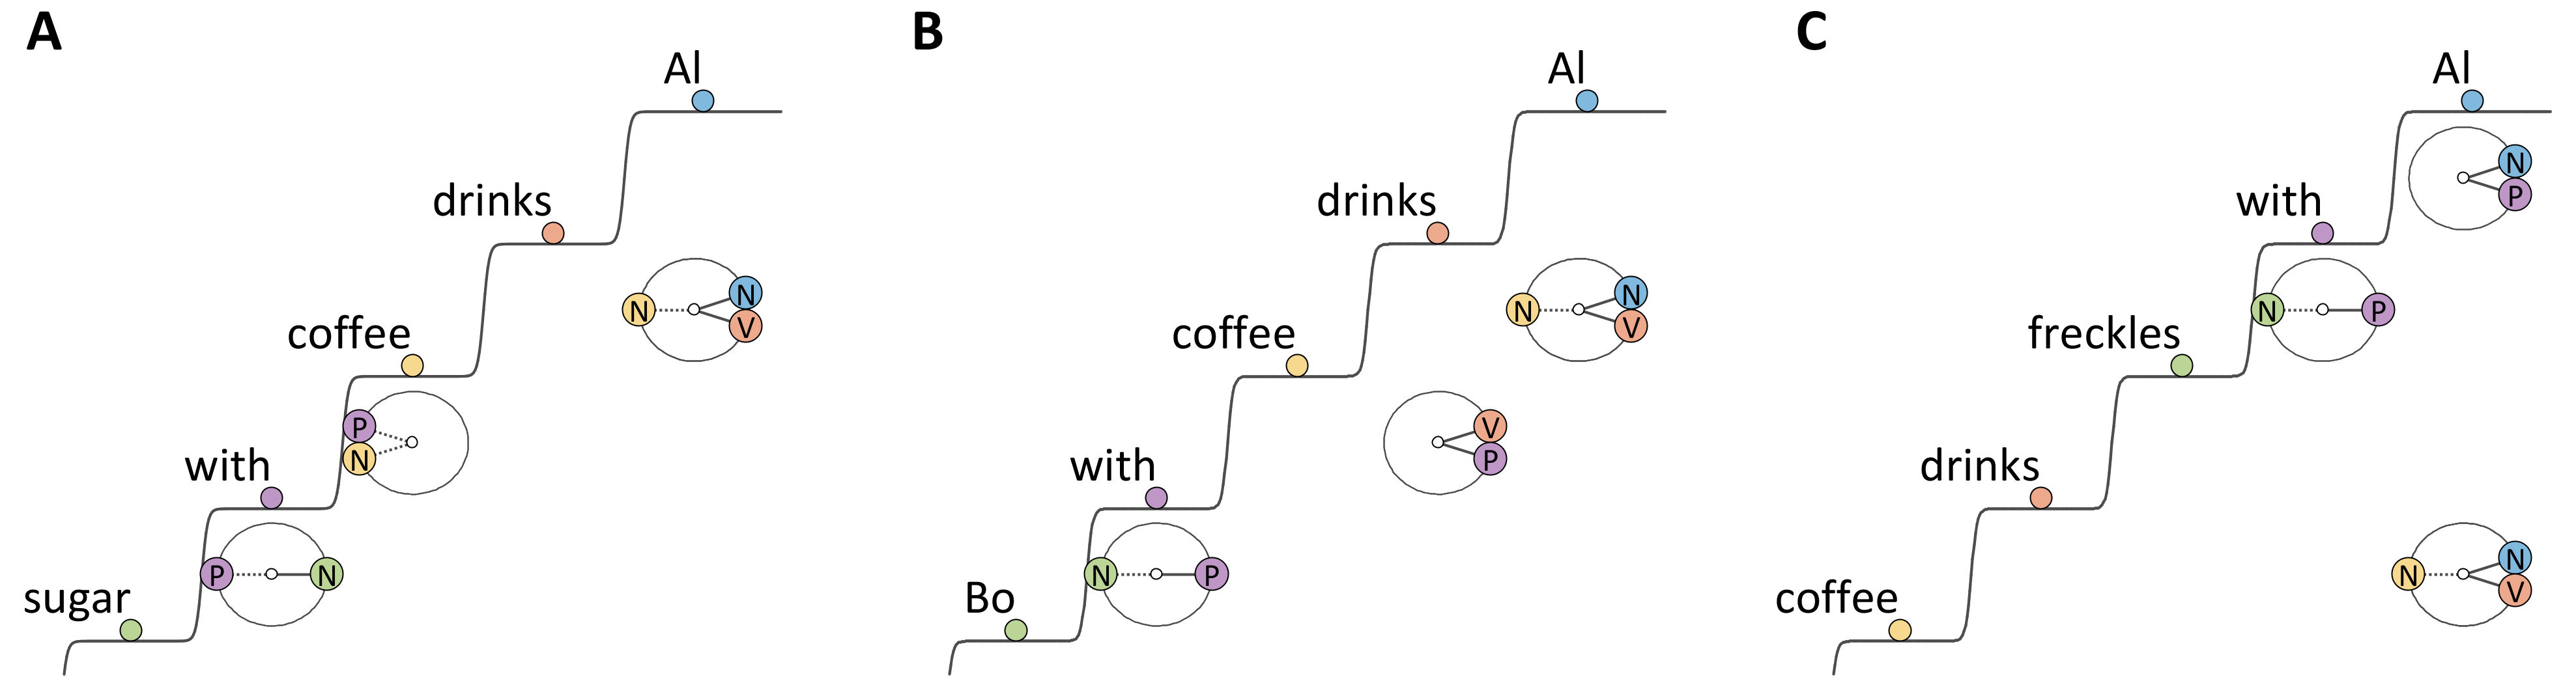
\includegraphics[width=\textwidth]{figures/Tilsen-img84.png}
\caption{\missingcaption}
\label{fig:4:34}
\end{figure}
 

  In contrast with phrasal uses of prepositional word forms, there are often particle/adverbial uses of the same word forms, which should not be analyzed as bivalent \{P\} because they do not relate two cs-systems. Consider the contrast between (A) and (B)/(C) below. In (A), \textit{up} is a \{P\} system and has a complement, [hill]\{N\}; it relates [runs]\{V\} to [hill]\{N\} and thus is bivalent. In the other two examples, \textit{up} is a particle s-system \{PRT\} and has no complement, its only φ relation is +φ coupling with [runs]\{V\}.

  
\begin{figure}
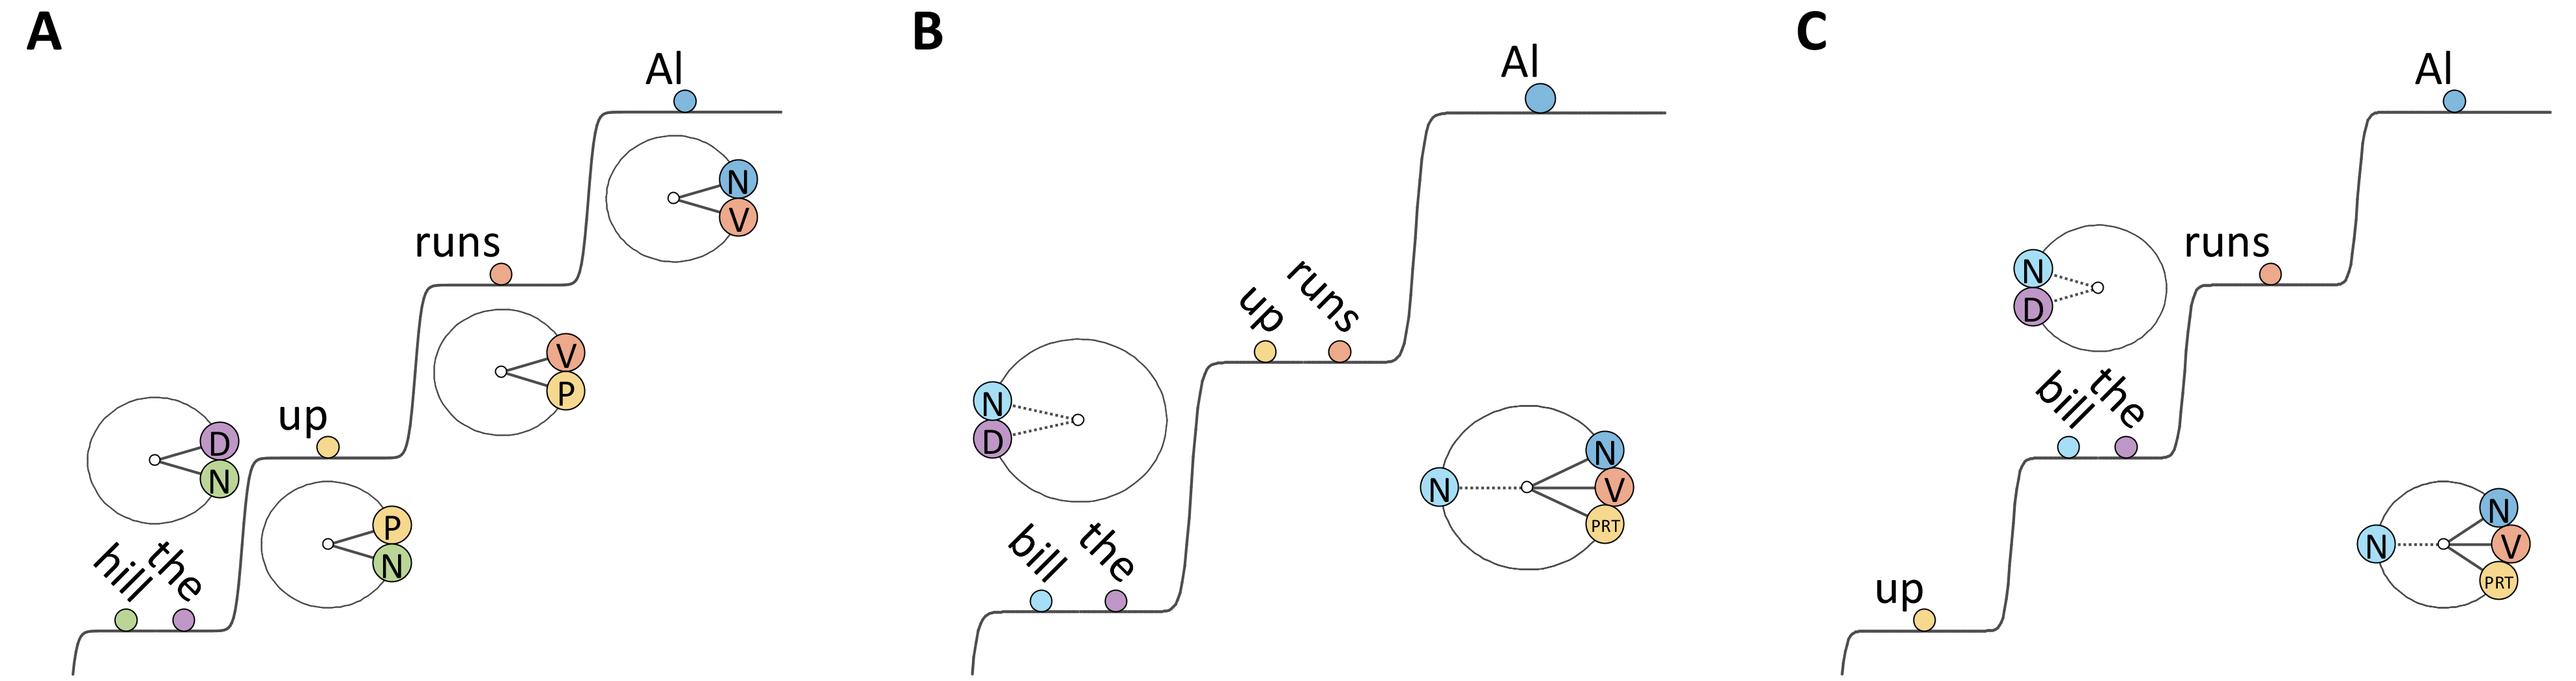
\includegraphics[width=\textwidth]{figures/Tilsen-img85.png}
\caption{\missingcaption}
\label{fig:4:35}
\end{figure}
 

  Based on the above examples, obligatoriness and optionality might seem to provide a reasonable basis for constructing a distinction between arguments and adjuncts. Specifically, we might propose that \{V\} systems obligatorily φ-couple to agentive and/or patientive systems, while \{ADV\}, \{ADJ\}, \{P\} systems are optional modifiers of \{V\} and \{N\} systems. We could elaborate this proposal by adding that some verbal cs-systems require -φ coupling to a recipient, e.g. \textit{Bo gave Al coffee}, and others require indirect coupling of an argument via \{P\}, e.g. the locative \textit{Al put coffee in the cup}, where \{P\} is +φ coupled to [put]\{V\} and -φ coupled to [cup]\{-N\}.

  However, the obligatoriness of these coupling relations is not so categorical. In many cases, verbal c-systems which are normally organized with \{-N\} systems occur in utterances where no such system is selected, e.g. \textit{Al drinks}. How should we analyze this phenomenon? One possibility is that no \{-N\} system is active, and a differentiation [drink\textsc{\textsubscript{intr}}]/[drink\textsc{\textsubscript{tr}}] occurs. Alternatively an [\textsc{intr}]\{\textsc{val}\} system couples to \{V\}, as shown in example (A). A different approach shown in (B) would be to construct a generic [\textsc{theme}]\{-N\} system and posit that this system is active but unexcited during the production. Recall that the canonical reorganization promotes only excited systems, so [\textsc{theme}] is never selected in this scenario. 

  
\begin{figure}
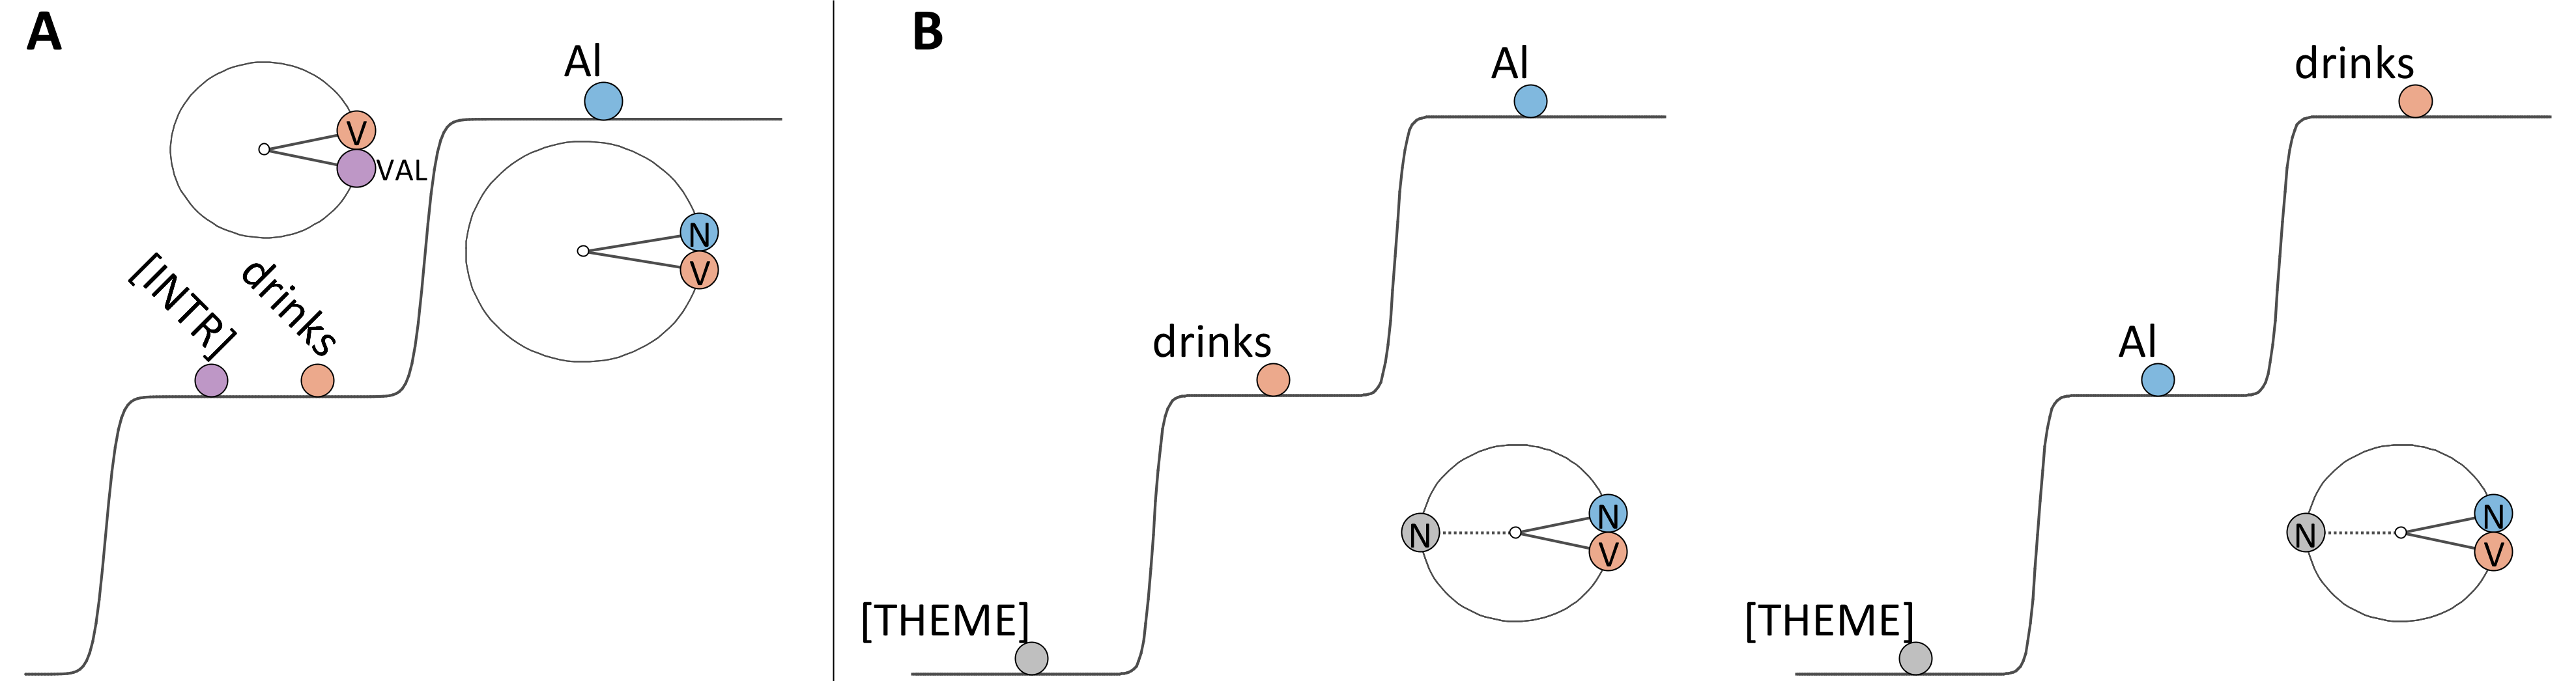
\includegraphics[width=\textwidth]{figures/Tilsen-img86.png}
\caption{\missingcaption}
\label{fig:4:36}
\end{figure}
 

  A third possibility (not shown) is that some cs-system is indeed excited, but the producer does not promote it to selection-level, i.e. a non-canonical reorganization occurs. How do we resolve between these analyses? One relevant observation is that for some verbal c-systems, omission of the argument can evoke an arbitrary conventional or contextual relational meaning. For example, \textit{Al drinks} is often understood to implying drinking of alcoholic beverages of some sort. \textit{Al smokes} can imply that Al smokes cigarettes, or something else, depending on the context. When a theme/patient c-system is sufficiently active from context, a producer may not excite the system or may not select it, and yet contextual forces induce the relevant φ configuration for an interpreter. For example, imagine a speaker says \textit{Al holds the coffee. He drinks.} The hearer will experience a {\textbar}Al drinks coffee{\textbar} trajectory because the omitted cs-system [coffee]\{N\} is sufficiently active from the first sentence.

  The above observations suggest that there are always active theme/patient c-systems in productions with omitted arguments, but these are not necessarily selected. The ground-level is our representational mechanism for indicating the presence of an active but unexcited cs-system. Thus we might analyze the implicit argument as unexcited, which is represented in (B) above. However, the principle of relational meaning holds that attended relational meaning experiences are evoked only by φ configurations in which all relevant cs-systems are excited; thus we should prefer an analysis in which a noncanonical reorganization causes the implicit argument not to be selected. This is shown below; the reorganization Ê\textsubscript{2} from (e1) to (e2) is canonical, but reorganization Ê\textsubscript{3} demotes [coffee] rather than promoting it to selection-level:

  
\begin{figure}
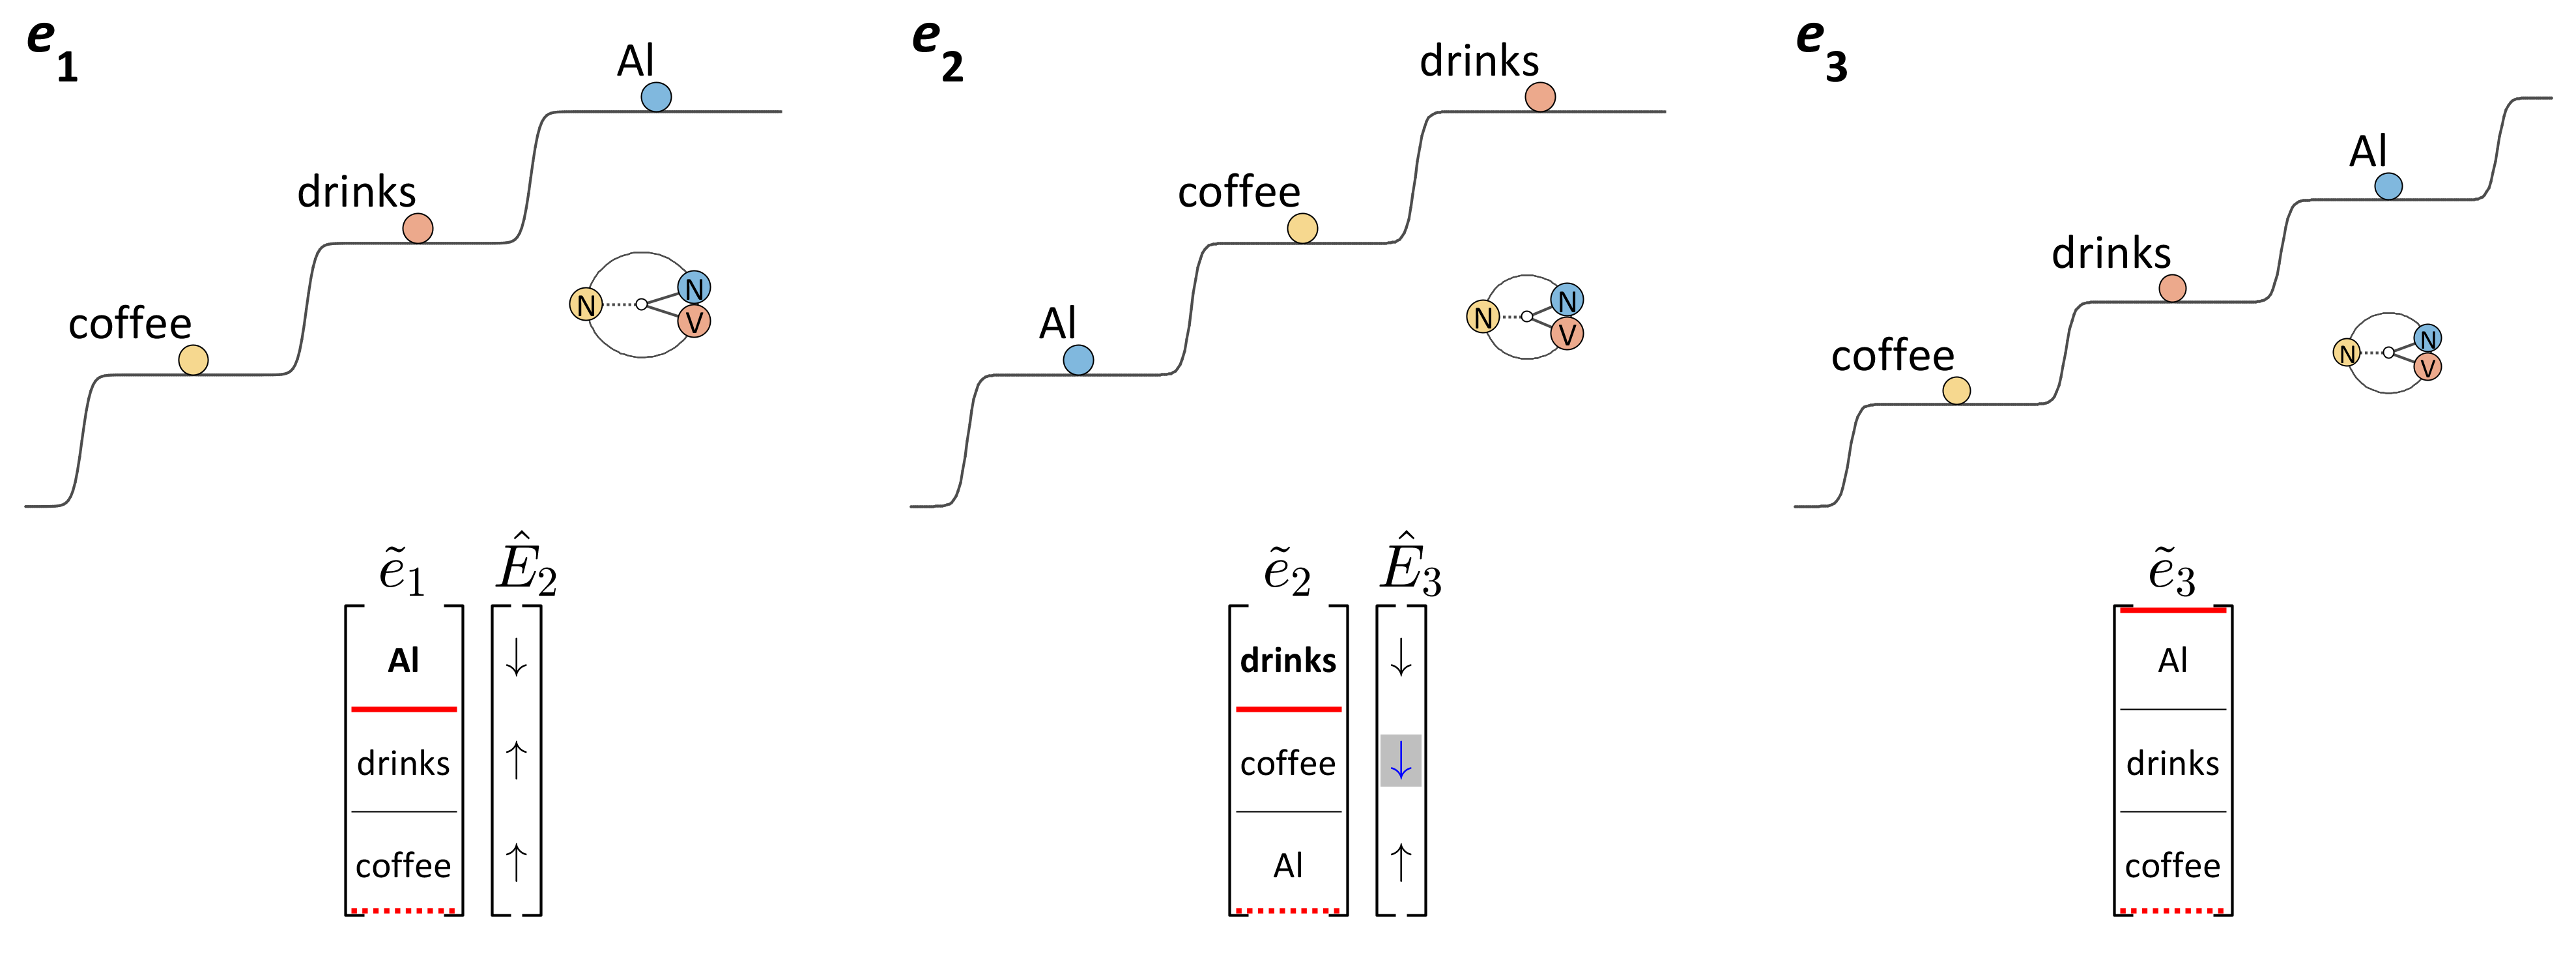
\includegraphics[width=\textwidth]{figures/Tilsen-img87.png}
\caption{\missingcaption}
\label{fig:4:37}
\end{figure}
 

  Overt and implicit argument patterns for the same φ configuration can be viewed as different state trajectories in e-subspace. Instead of dichotomizing between properties of obligatoriness and optionality for arguments, we argue that the noncanonical reorganization associated with implicit arguments occurs due to aspects of the state (e2) which are not explicitly represented. In general, we can imagine a high-dimensional θ/e/\textit{f} space for a large number of c- and s-systems, along with a time-dependent surroundings forces on each system. For any given state at time \textit{t}\textsubscript{s}, there is a source volume in state space, i.e. a state space region at time \textit{t}\textsubscript{0} from which the system evolves to the given state at time \textit{t}\textsubscript{s}. For multiple states we can imagine their relative source volumes. 

  Given this construct, the distinction between obligatoriness and optionality can be reconceptualized as difference in the relative source volumes of trajectories in which some cs-system is or is not selected. A 1-dimensional analogue of the state space volume is shown in the {\figurebelow}. At \textit{t}\textsubscript{0} we compare the volumes of the regions of state space from which trajectories evolve to a canonical or noncanonical reorganization: 

  
\begin{figure}
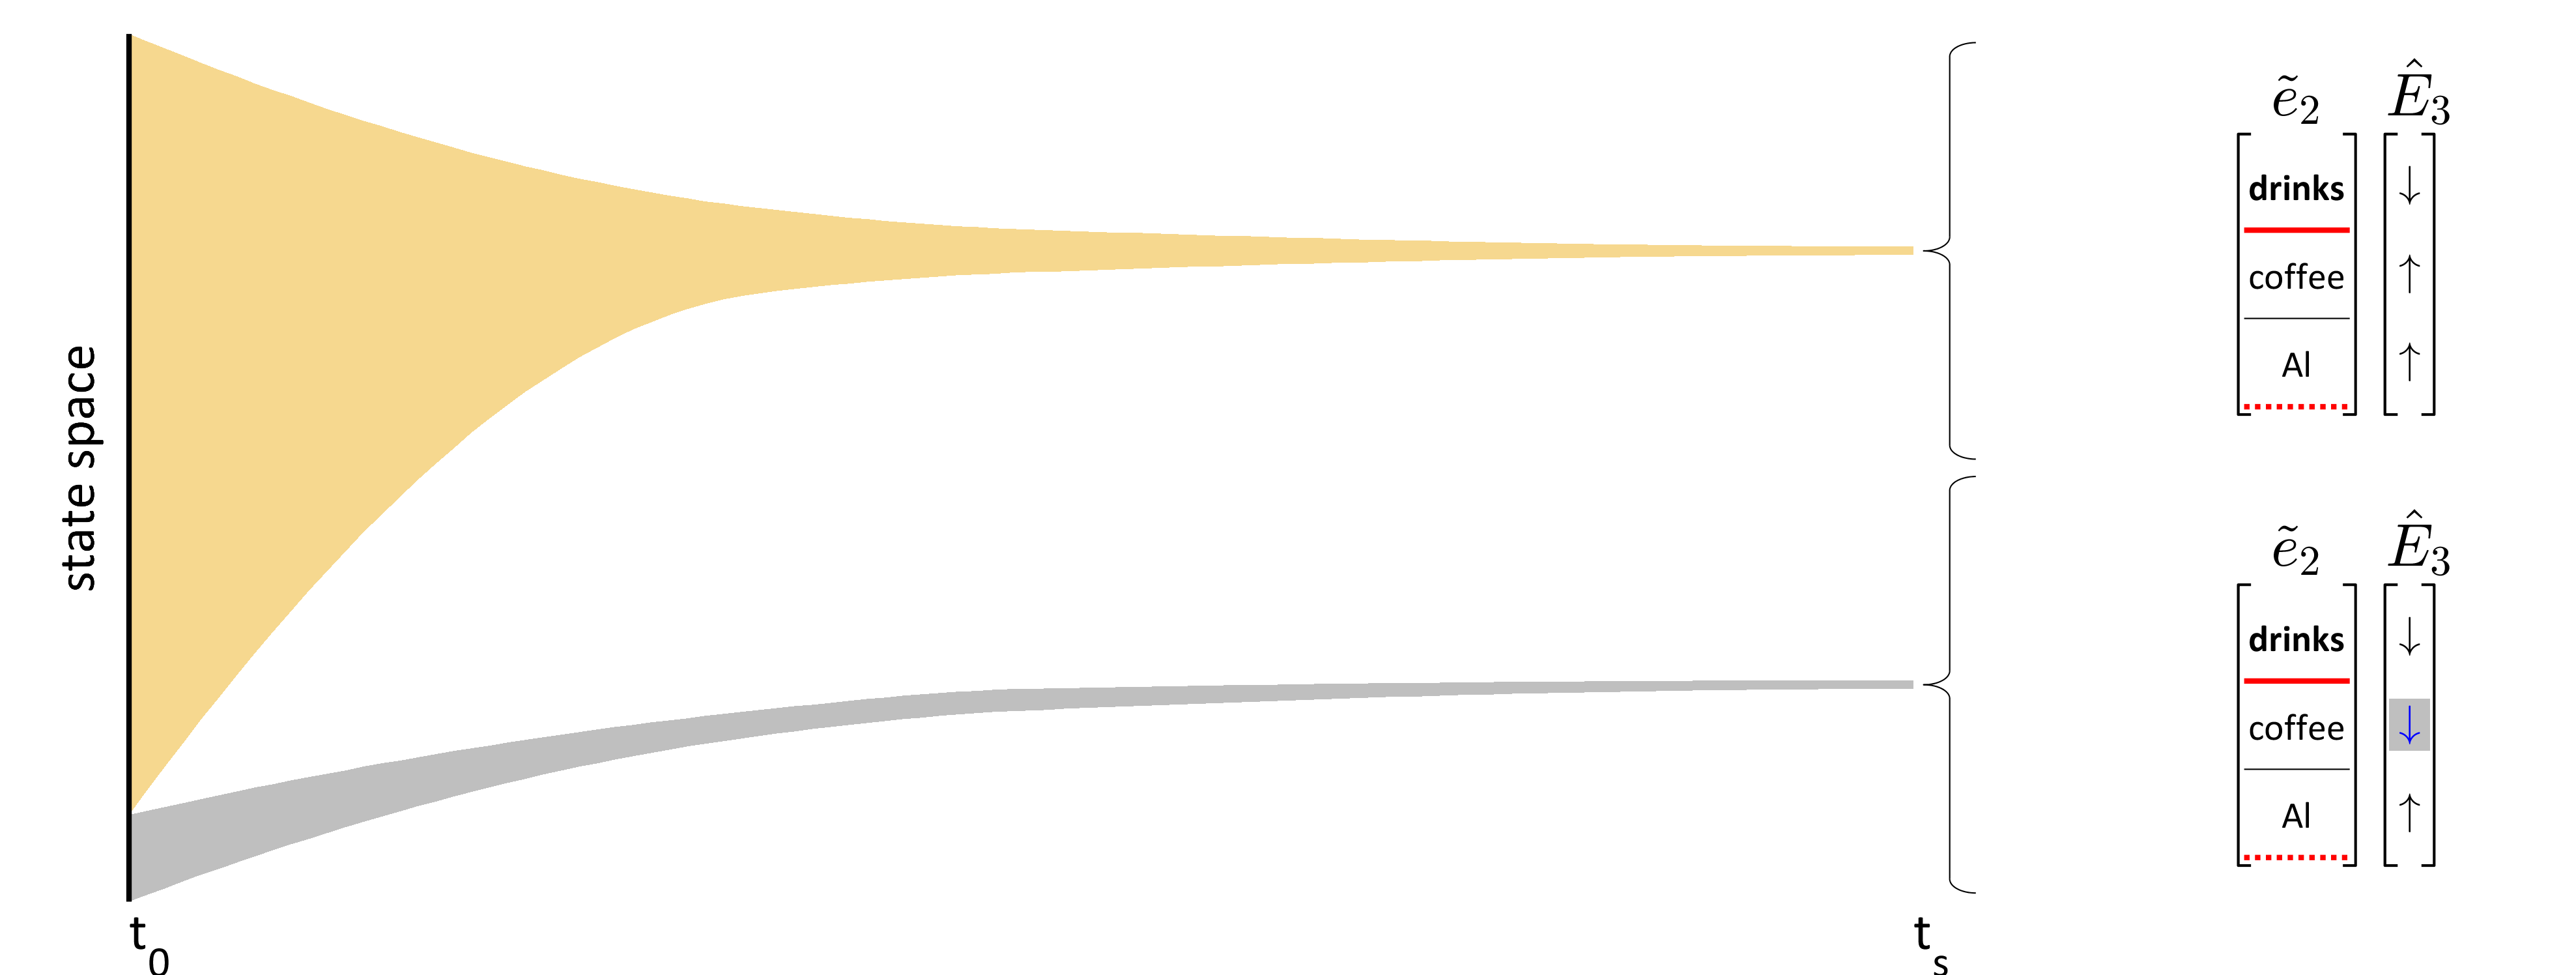
\includegraphics[width=\textwidth]{figures/Tilsen-img88.png}
\caption{\missingcaption}
\label{fig:4:38}
\end{figure}
 

  From this perspective the concepts of obligatoriness and optionality are misleading: the likelihood of argument omission derives from the relative source volume of the noncanonical reorganization. The identity of active c-systems is an important dimension but many other surroundings-related forces may also contribute: argument optionality/obligatoriness cannot be construed solely as a function of the states of systems which are explicitly constructed in a given analysis.

\subsection{Configurational ambiguity}

Ambiguity is an analytic construct which cannot be defined without arbitrary constraints. It inherently  involves both production and interpretation, the latter of which we have mostly neglected so far. It is tempting to define ambiguity as a property of an utterance such that multiple configurations \textit{could} be evoked in the interpretation of an utterance. But all utterances are ambiguous under this definition, because surroundings forces can bias an interpreter toward a trajectory in which relational meaning differs arbitrarily from the intentions of the producer. In practice analyses of ambiguity often assume some degree of similarity between a production trajectory and potential interpretation trajectories—these are the more interesting cases, perhaps. However, defining \textit{similarity} in this context is never attempted. For current purposes, we assume that interpreters perceive gm-systems which activate the same cs-systems as those which are active for a producer, this process occurring through learned gm-to-cs mappings. Of course, one can analyze ambiguity in gm-to-cs mappings as well—cf. \textit{excuse me while I kiss this guy} vs. \textit{excuse me while I kiss the sky}—but here our focus is on cs-configurational ambiguity. 

  It is important to recognize that ambiguity relates to \textit{potential} interpretation states. Actual interpretation states cannot be ambiguous, nor can production states. Non-ambiguity of states follows from our conceptual model: there is just one system and one state trajectory for a given period of time for a producer or interpreter. Simultaneous distinct state trajectories are not possible, nor are state trajectories probabilistic. All utterances may be ambiguous, but states are never ambiguous; we therefore view ambiguity as an analytical choice to imagine how different interpreter trajectories could be evoked by the same production trajectory.

  Consider a classic example of ambiguity: \textit{Al saw the man with the telescope}, which can evoke the interpretation in (B) or (B′) below. Our phrasal organization hypotheses entail that a configuration such as (A), which would purportedly evoke both interpretations, cannot be stable. Recall that bivalent \{P\} relates a modificand and complement by +φ and -φ coupling to each of these, respectively. For both the (B) and (B′) interpretations, \{P\} must be -φ coupled to its argument, [telescope]\{N\}. However, for the interpretation in (B), \{P\} must be +φ coupled to [saw]\{V\}, and for (B′), \{P\} must be +φ coupled to [man]\{N\}. But note that these two potential modificands, [saw]\{V\} and [man]\{N\}, have a -φ relation (because of the φ invariance principle). Thus there is a conflict between the configurations in (B) and (B′): in order for \{P\} to +φ couple with both modificands and be in a -φ configuration with [telescope]\{N\}, either \{P\} or [telescope]\{N\} would need to be in both θ and θ+π states simultaneously, which violates our deterministic construal of the system. Another way to describe the problem is to say that φ-coupling between \{P\} and [saw]\{V\} has destructive inference with φ-coupling between \{P\} and [man]\{-N\}. Hence only one of the configurations (B) or (B′) can arise.

  
\begin{figure}
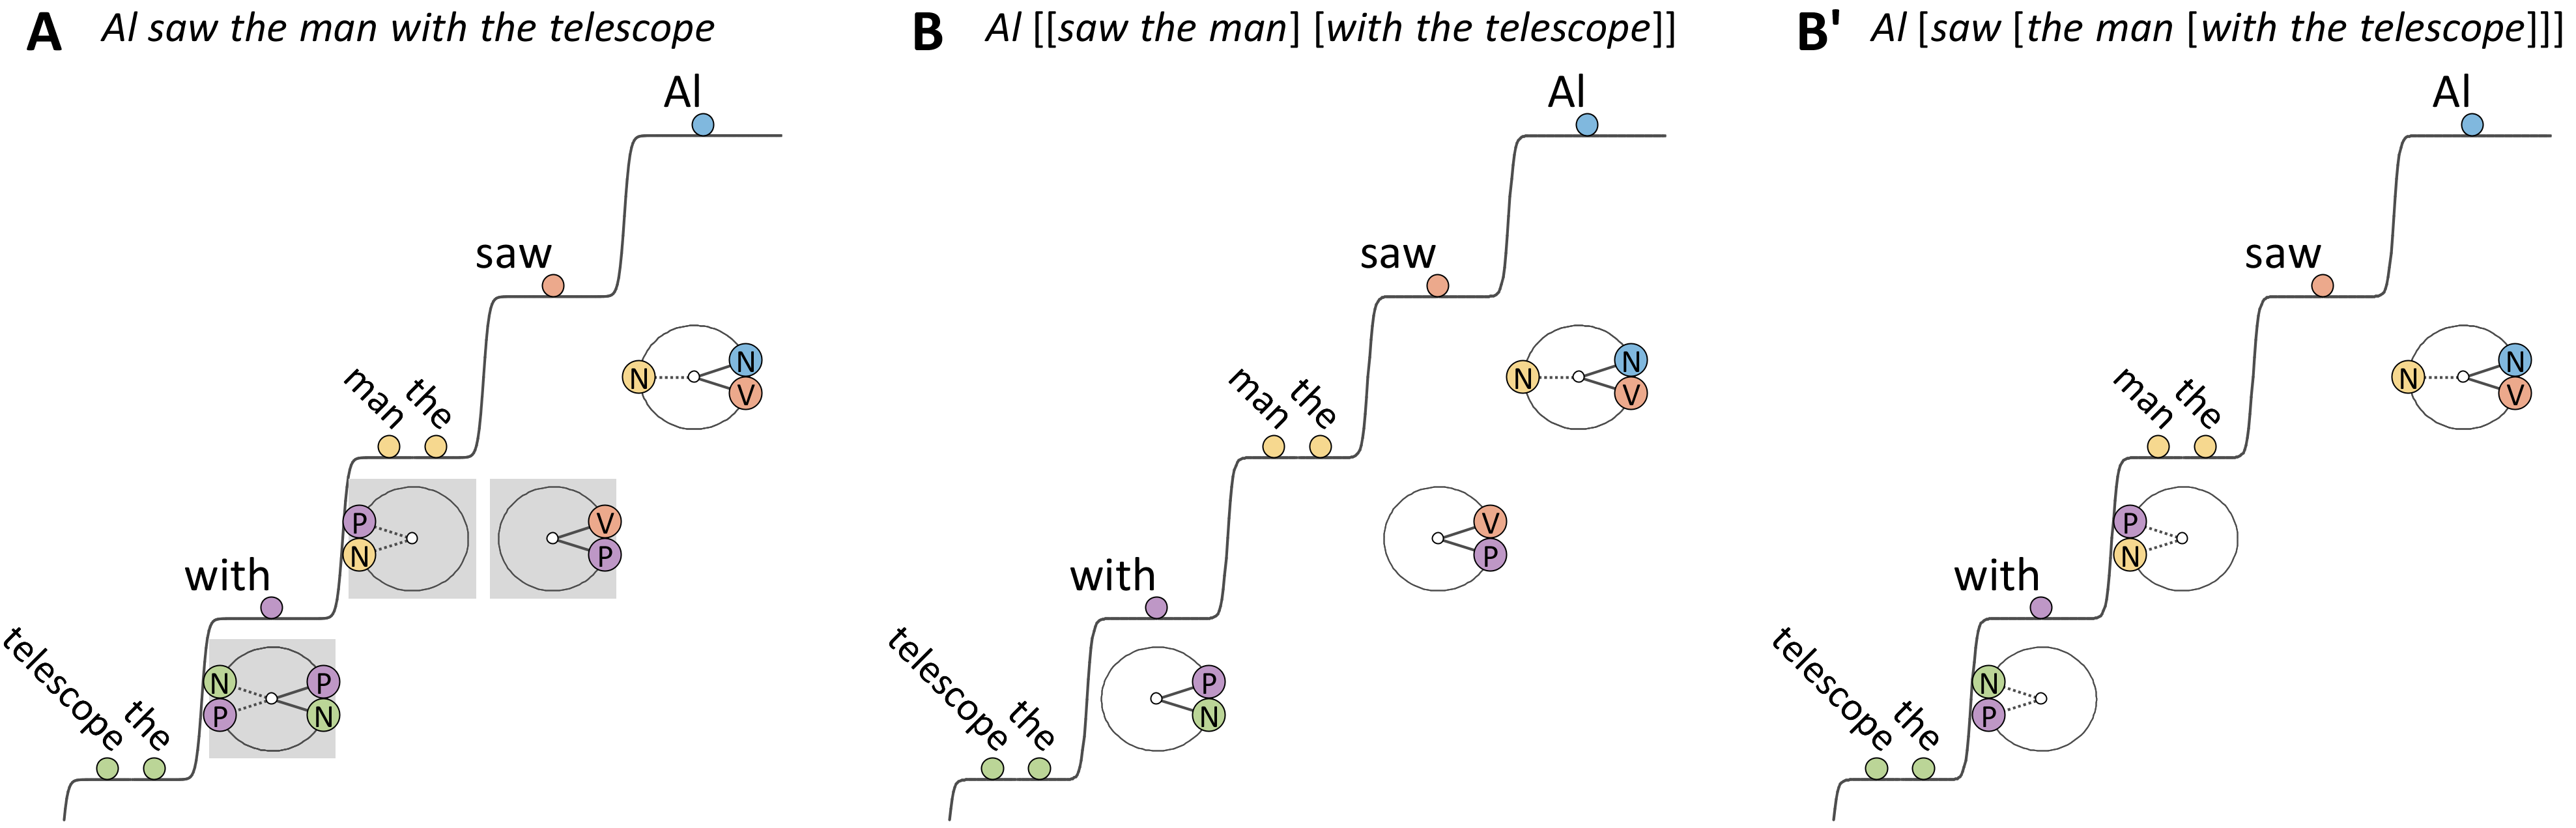
\includegraphics[width=\textwidth]{figures/Tilsen-img89.png}
\caption{\missingcaption}
\label{fig:4:39}
\end{figure}
 

  In production, ambiguity is irrelevant because surroundings forces are deterministic and thus drive the emergence of a unique φ configuration. But to understand interpretation (including self-interpretation of a recently produced utterance), we need to understand the mechanisms through which φ configurations stabilize when evoked cs-systems could obtain multiple possible configurations. This becomes particularly relevant when we consider grammaticality intuitions and various syntactic phenomena in later chapters.

  As a starting point, we ask whether there are any obvious differences between stabilization mechanisms in interpretation and those we have hypothesized for production. Recall that in the canonical production trajectory φ configurations stabilize before e-organization. Does this apply to a canonical interpretation trajectory as well? Two possibilities are contrasted below. In both, sensory systems are viewed as surroundings forces which activate cs-systems, based on veridical, non-ambiguous cs-to-gm mappings. In the first scheme, a stable e-organization, if one arises, does so only after a φ-organization stabilizes: no form of e-organization is stable prior to φ-stabilization. This scheme conceptualizes interpretation as similar to production.

  
\begin{figure}
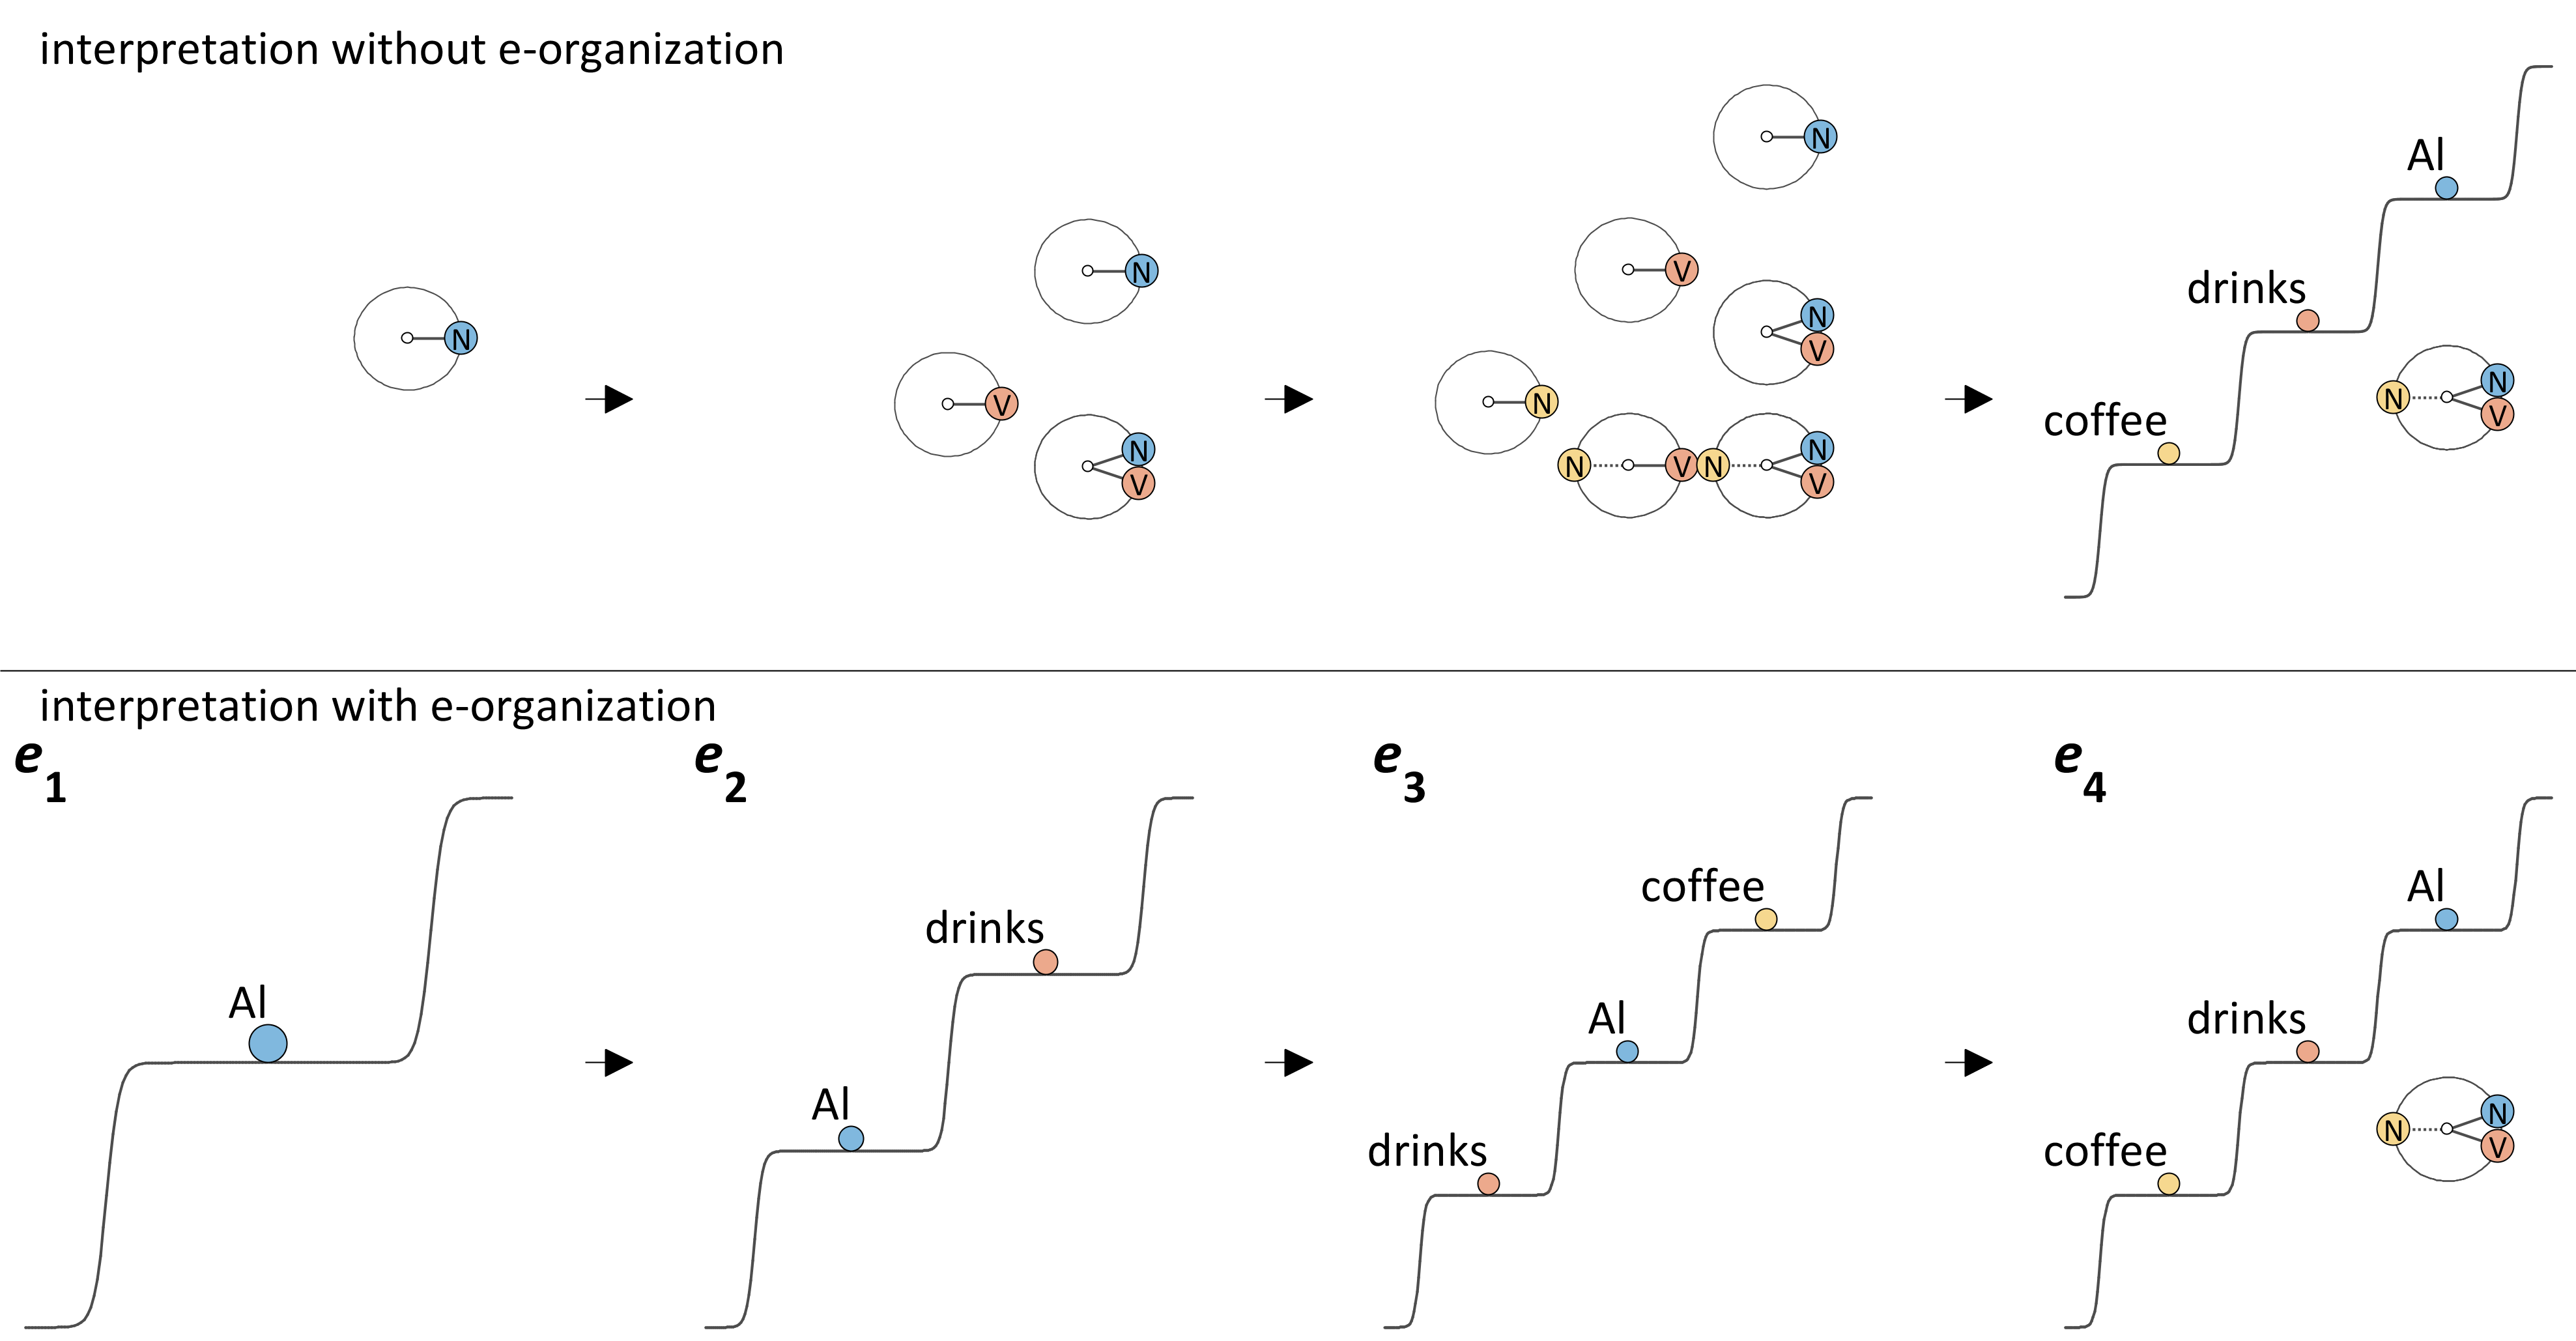
\includegraphics[width=\textwidth]{figures/Tilsen-img90.png}
\caption{\missingcaption}
\label{fig:4:40}
\end{figure}
 

  In the second possibility, systems are e-organized and reorganized incrementally while φ configurations evolve. The question of precisely how the e configurations might reorganize over the course of interpretation is challenging. One possibility shown above combines the canonical reorganization operator Ê\textsuperscript{cr} with a mapping of the most recently perceived cs-systems to the highest e-level. For example, in epoch (e3) when [coffee]\{N\} is activated, it becomes sufficiently excited so as to occupy the highest e-level, while the system which previously occupied the highest level, [Al]\{N\} is demoted and all other systems are promoted. This particular mechanism of e-organization in interpretation has the advantage that the final organization is identical to the initial e configuration that produces the utterance. However, the alternative in which e-organization does not occur incrementally cannot be ruled out, and later on we find it more appropriate for understanding electrophysiological responses in sentence comprehension paradigms.

  In either conceptualization of interpretation, we must allow for φ configurations to emerge flexibly from surroundings forces. Incremental e-organization during interpretation may attribute too much order to interpretation trajectories, but it helps us reason about how the current e-state may influence the φ-state. One important point here is that canonical production not does not appear to be subject to this dilemma. Different e-states in production may arise from a given φ configuration, but the reverse does not hold: φ configurations in production trajectories are not canonically influenced by e-states. The mechanism that prevents incompatible φ coupling patterns from being stable simultaneously is interference, which we now turn our attention to.

\section{Interference}

Our derivation of a macroscopic model from a microscopic one holds that systems are collective oscillations of finite populations of neurons. As we argue below, the finite nature of this microscale substrate entails that there are limits on the number of macroscale systems which can be simultaneously excited. The mechanism which is responsible for these limitations is \textit{interference}, and below we describe two classes of interference that affect system stability, \textit{differentiation interference} and \textit{configurational interference}. Importantly, differences in excitation can mitigate the destabilizing effects of interference. Excitation differences are viewed as a mechanism for selectively attending to some configurations instead of others, and we argue that selective attention provides a solution to the multiplicity problem.

\subsection{Limits on organization}

To explain how differentiation interference arises, lets consider differentiation on the microscale. We begin by identifying \{X\} as the finite population of neurons which comprises all s-system populations. In order for different classes of s-systems to be simultaneously active, the \{X\} population must be differentiated into subpopulations such as \{V\}, \{\textsc{adj}\}, \{\textsc{adv}\}, \{+N\}, \{-N\}, etc. But what do these differentiations entail on the microscale?

  In addressing this question, we distinguish differentiation on two timescales. On developmental timescales, changes in connectivity and in the strengths of synaptic interactions can create relatively independent subpopulations of \{X\}, which do not strongly interfere with each other. The basic lexical categories of a language, i.e. \{V\}, \{\textsc{adj}\}, \{\textsc{adv}\} \{+N\}, \{-N\}, \{\textsc{tns}\}, \{\textsc{person}\}, \{\textsc{number}\}, etc. are likely to be differentiated in this way on developmental timescales. These differentiations are motivated by differences in c-systems, which in turn arise from differences in patterns of sensorimotor interaction. In other words, \{V\} and \{N\} subpopulations of \{X\} arise because they are coupled with c-systems that differ by virtue of their surroundings connectivity. Developmental scale differentiations do not give rise to strong interference.

  On the utterance timescale, differentiation creates subpopulations which are not strongly independent and which can interfere strongly. Utterance timescale differentiation cannot change connectivity or cause drastic changes in synaptic interaction, and so if a population differentiates in this way, it must occur through a more temporary mechanism, such as phase and/or frequency differentiation, which we conceptualize as follows. Imagine two c-systems, [y1] and [y2] which resonate with an s-system \{x\}. When both [y1] and [y2] are active, \{x\} differentiates into two subpopulations, \{x1\} and \{x2\}, hence there are cs-populations [y1]\{x1\} and [y2]\{x2\}. We infer that \{x1\} and \{x2\} populations cannot be identical, otherwise the meaning experiences associated with [y1] and [y2] would not be distinct. How then, is the differentiation accomplished? 

  Note that the population oscillations of [y1] and [y2] do not in general have the same intrinsic frequencies \textit{f} and do not become active (begin to oscillate) at identical times; hence the phase velocities θ′ and phases θ of the c-systems typically differ in pre-stable phases of production. If the neurons of [y1] and [y2] had identical, equally strong projections to neurons of \{x\}, then the differences in c-system θ/θ′ would exert conflicting forces on \{x\}, which could not be stable. However, if projections from [y1] and [y2] to \{x\} are different (even if for random reasons), then there will be a subpopulation \{x1\} which is more strongly influenced by projections from [y1], and a subpopulation \{x2\} more strongly influenced by projections from [y2]. Because of these asymmetric influences, the \{x1\} and \{x2\} subpopulations may attain different θ/$\theta ′$ states that accord with the θ/$\theta ′$ states of [y1] and [y2]. In other words, \{x\} as a whole exhibits phase and phase velocity heterogeneity: the oscillations of spike rates of subpopulations \{x1\} and \{x2\} may be out of phase by an arbitrary amount and may be at different frequencies. It is an open question whether utterance timescale differentiation is accomplished primarily by maintaining a θ′ difference (frequency modulation) or a θ difference (phase modulation), or some combination of both. (Note that our prior construal of the developmental scale \{+N\}/\{-N\} differentiation assumed a phase modulation).

  By definition, θ/$\theta ′$ heterogeneity of differentiated subpopulations \{x1\} and \{x2\} is “interference” because the subpopulations interact. The crucial question is not whether interference exists, but whether the interference is destabilizing. This depends on several microscale factors. One is the number of projections between subpopulations and their synaptic strengths. If the interaction is too strong, θ/$\theta ′$ heterogeneity of \{x1\} and \{x2\} destabilizes the systems. Another factor is the degree of asymmetry in the interactions between [y1]/[y2] and the s-system populations: if the influence of [y1]\{x1\} interaction relative to [y1]\{x2\} interaction is large, and vice versa the influence of  [y2]\{x2\} interaction is large relative to [y2]\{x1\}, conditions are favorable for stabilizing the differentiation.

  A third factor is the number of differentiations which occur. With each differentiation, the number of neurons in each subpopulation becomes smaller, and there will be more variation in the θ/$\theta ′$ values of the interacting populations. Moreover, the influence of interactions with other populations becomes stronger relative to the internal forces which stabilize the oscillation of each subpopulation.  Although we do not assume that differentiations are spatially organized, for convenience we can imagine that the differentiations increase population overlap, as represented below. As more differentiations occur, the proportional overlap of subpopulations increases, and consequently interference forces become stronger relative to stabilizing forces.

  
\begin{figure}
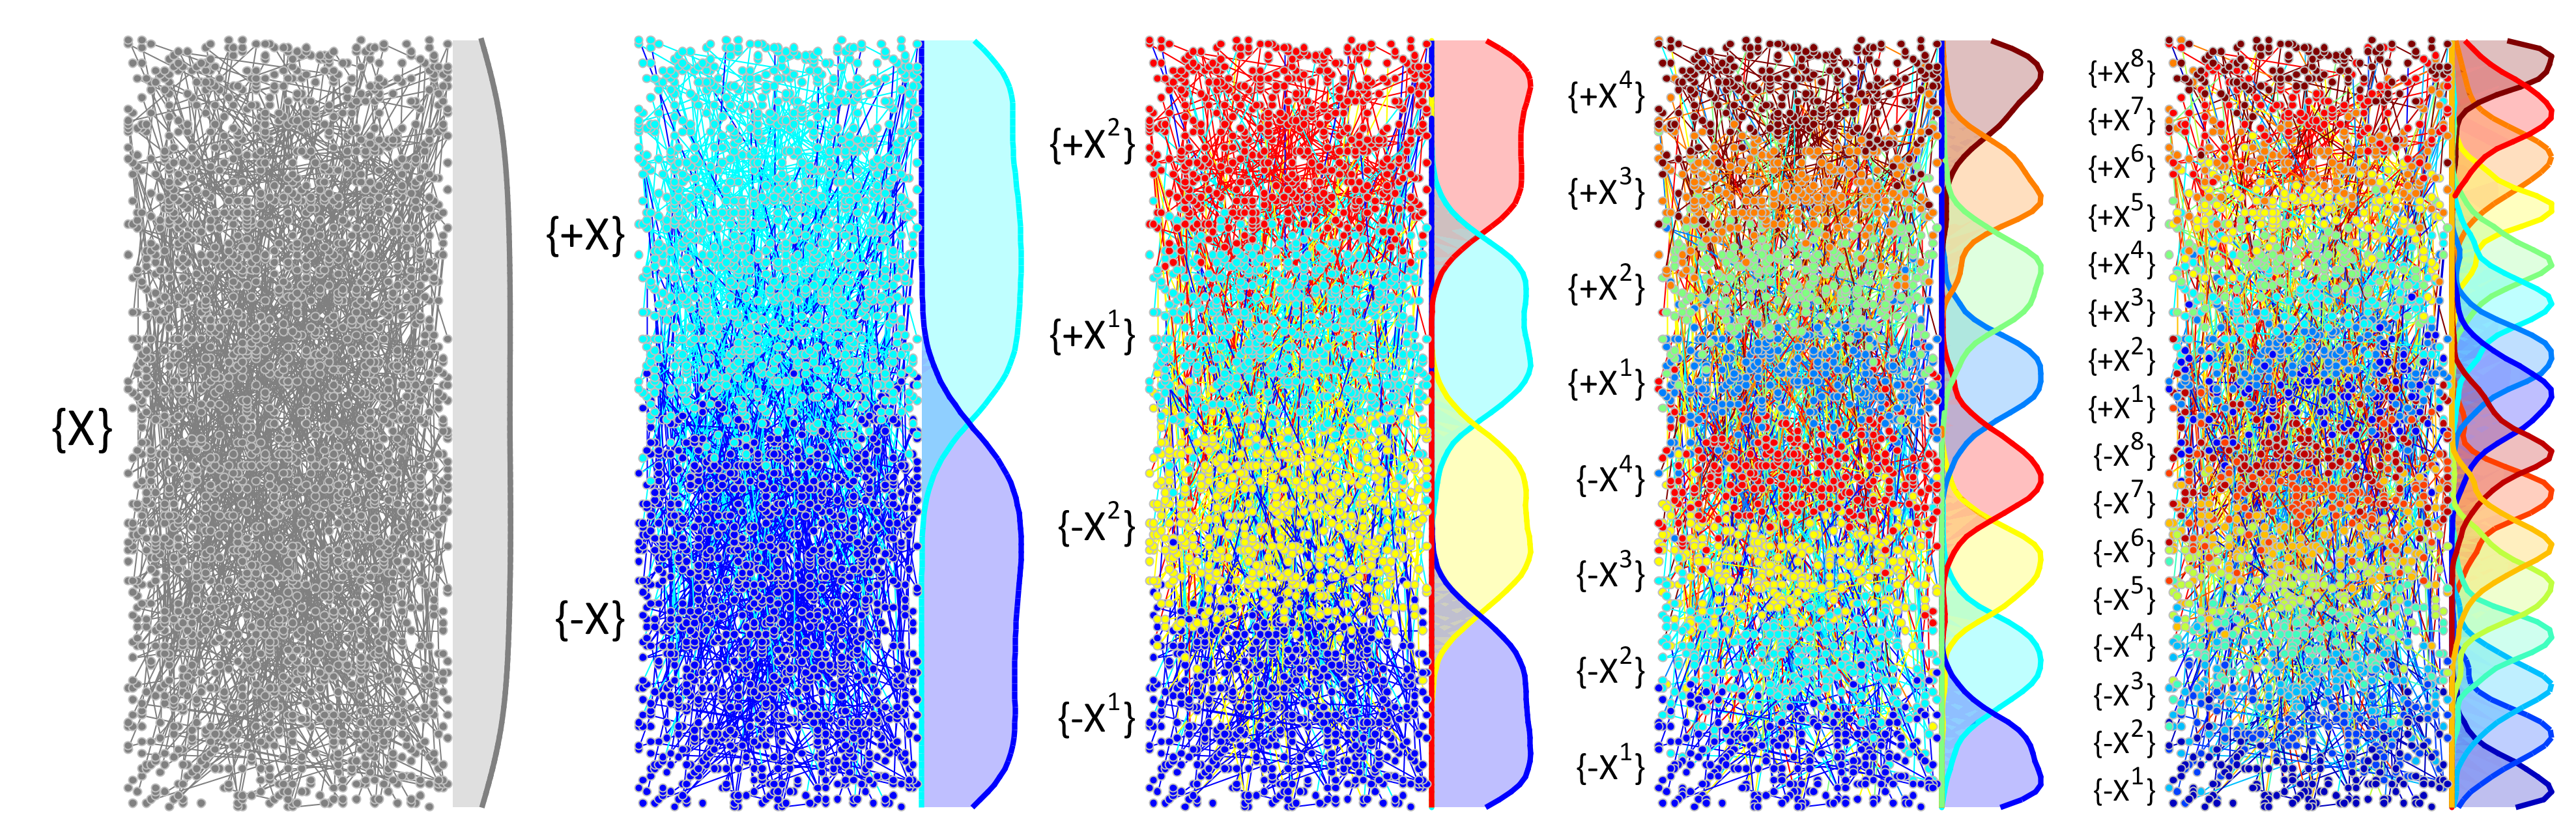
\includegraphics[width=\textwidth]{figures/Tilsen-img91.png}
\caption{\missingcaption}
\label{fig:4:41}
\end{figure}
 

  For a more concrete example, lets consider an utterance in which there are three c-systems, [c1], [c2], and [c3] that resonate with \{-N\}, e.g. \textit{Al drinks coffee, tea, and whisky}. In order for all three cs-resonances to be excited, this requires a stable differentiation of \{-N\} into \{-N\textsuperscript{1}\}, \{-N\textsuperscript{2}\}, and \{-N\textsuperscript{3}\} populations. We assume that [c1], [c2], and [c3] project non-uniformly to \{-N\}, and hence the differentiation \{-N\textsuperscript{1}\}, \{-N\textsuperscript{2}\}, and \{-N\textsuperscript{3}\} is possible. In the pre-stable phase when [c1], [c2], and [c3] become active, their phase velocities differ and their phases are not aligned. Because of the c-system θ/θ′ heterogeneity, the interaction forces from [c1], [c2], and [c3] to \{-N\textsuperscript{1}\}, \{-N\textsuperscript{2}\}, and \{-N\textsuperscript{3}\} induce destructive interfere between the s-system subpopulations. All three cs-systems cannot be highly excited, because this would result in strong destructive interference between \{-N\textsuperscript{1}\}, \{-N\textsuperscript{2}\}, and \{-N\textsuperscript{3}\} subpopulations. On this basis we infer that finite population size imposes limits on the number of distinct cs-resonances that can be simultaneously excited.

  
\begin{figure}
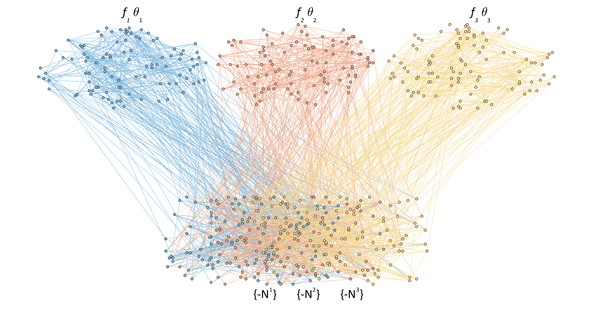
\includegraphics[width=\textwidth]{figures/Tilsen-img92.png}
\caption{\missingcaption}
\label{fig:4:42}
\end{figure}
 

  To better understand why interference is important for stability, lets expand our macroscopic conceptualization of \textit{x}\textsubscript{osc}, the oscillatory component of the system order parameter. Instead of imposing a single frequency on each system, we associate each system with a power spectrum and assume that there is a small range of frequencies over which there is non-negligible spectral amplitude of \textit{x}\textsubscript{osc}. In general what we expect to happen to an s-system as an active cs-resonance becomes excited is a narrowing of the spectral peak associated with the oscillation.

  
\begin{figure}
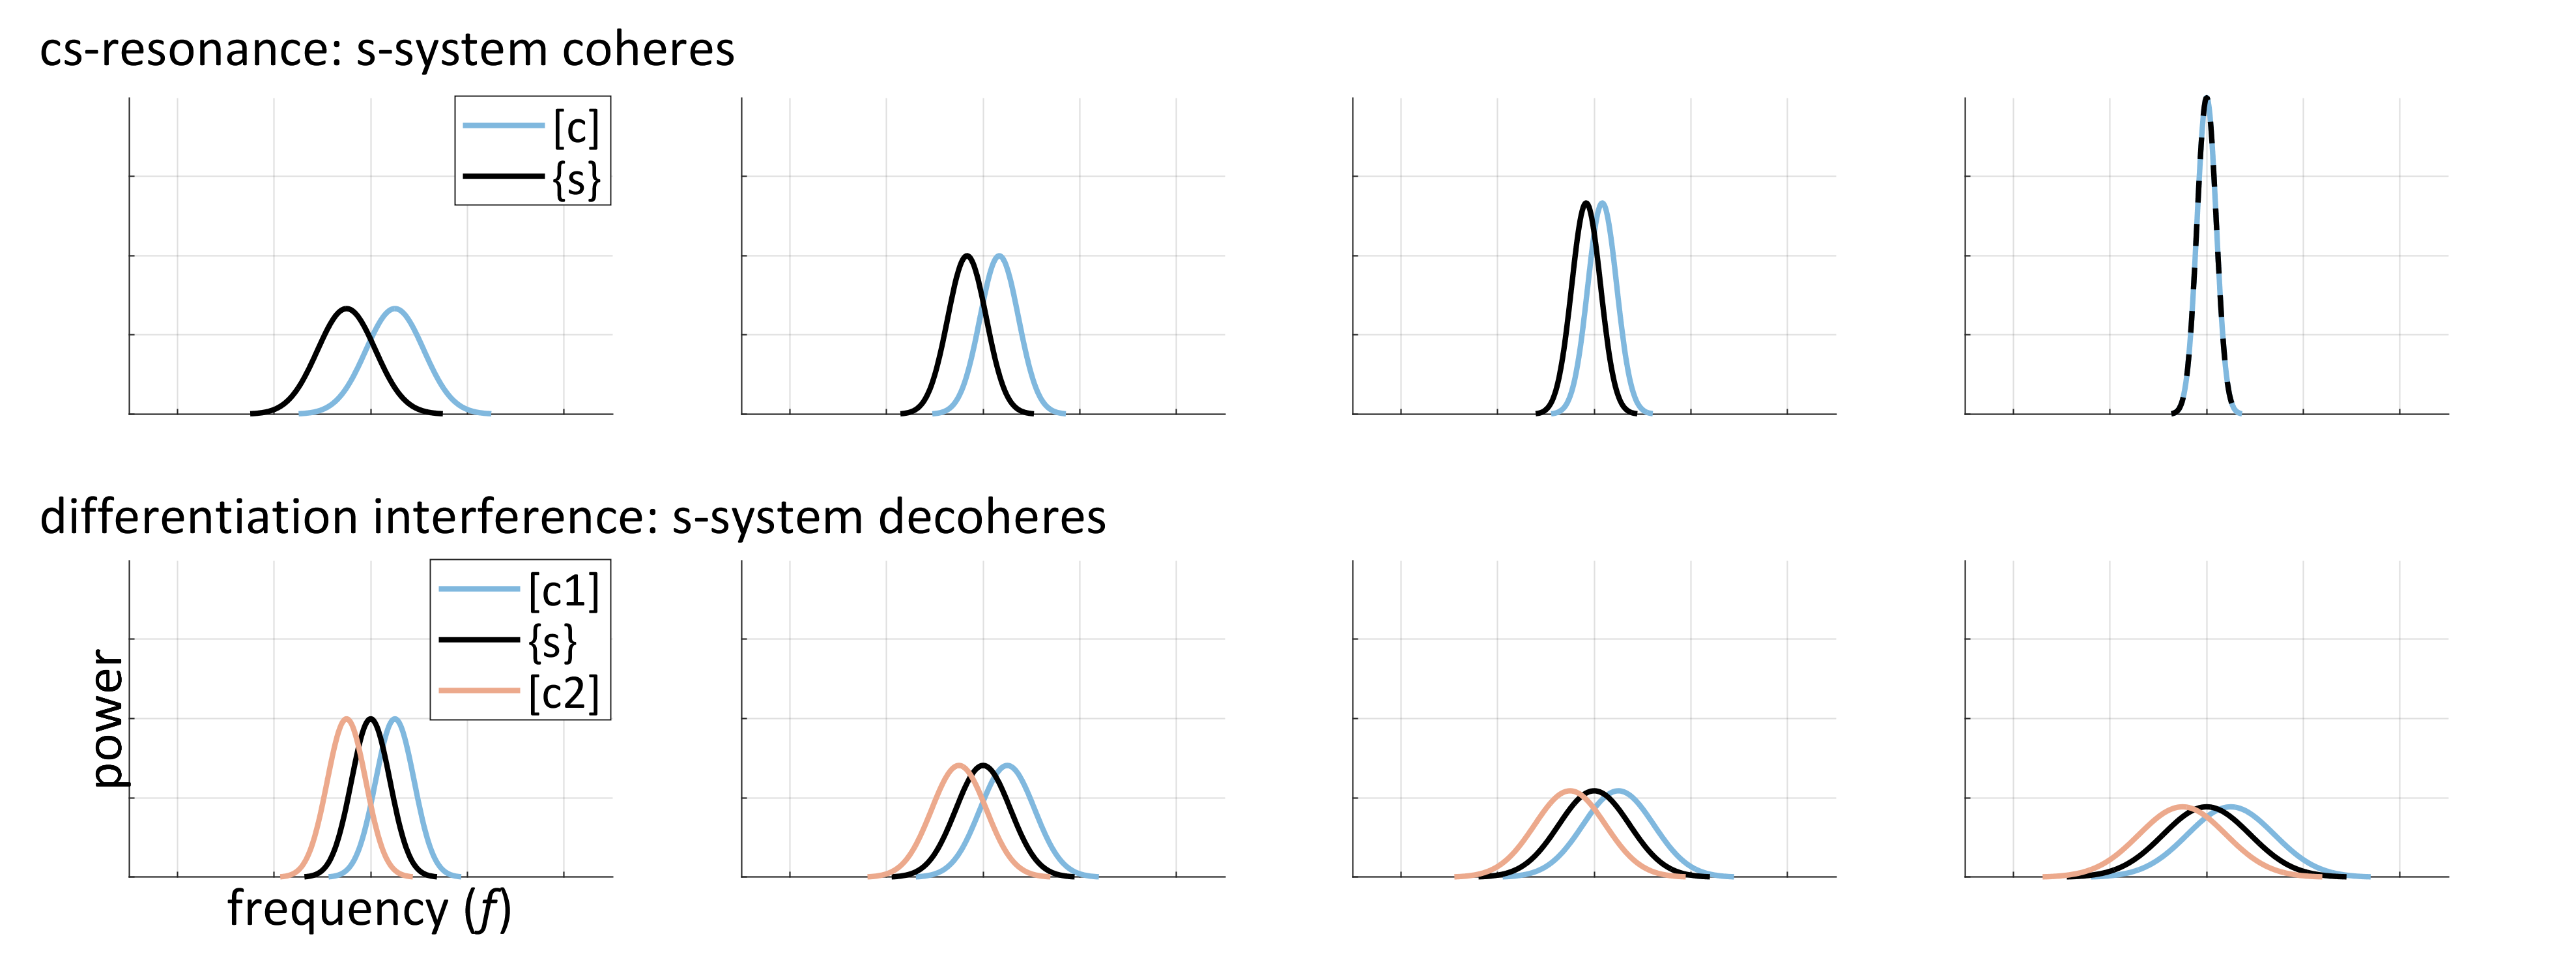
\includegraphics[width=\textwidth]{figures/Tilsen-img93.png}
\caption{\missingcaption}
\label{fig:4:43}
\end{figure}
 

  For each system, coherence corresponds to a narrowing of a peak in the power spectrum of \textit{x}\textsubscript{osc}, which occurs over some local period of time. We can take the width of this peak as a time-varying \textit{coherence measure}. In the absence of external forces, we imagine that systems tend to decohere. In cs-resonances, c-systems and s-systems exert coherence-promoting forces on one another. This causes their spectral peaks to approximate and narrow, as shown in the top row above. However, when multiple c-systems interact symmetrically with the same s-system, unless the spectra of those c-systems happen to be very similar, they will induce decoherence in the s-system, as in the bottom row of the figure. The extent to which the c-systems have a destabilizing effect on the s-system should depend on their cross-spectral coherence, γ\textsuperscript{2}(\textit{f}), over the relevant range of frequencies. Spectral coherence (Fourier transform of the autocorrelation) and cross-spectral coherence (Fourier transform of the cross-correlation) are tools for reasoning about what happens to population oscillations as systems cohere or decohere over time. However, for coherence to be applied quantitatively, a more detailed macroscale conception of system states is necessary, in which systems are associated with not just a single frequency, but rather a distribution of power over a range of frequencies. Later on we develop a reconceptualization of grammaticality and acceptability intuitions based on the coherence of excited cs-systems.

\subsection{Interference classification}

The classification of interference is useful for predicting whether a given configuration is more or less likely to be stable. We cannot make specific predictions regarding stability without hypothesizing values of certain parameters and conducting numerical simulations. We can, however, use our understanding of interference to draw inferences about the relative likelihood of various configurations being stable.

  To develop the classification, we first distinguish between interference and the more general concept of interaction. Interference requires at least three systems, whereas interactions are pairwise. In order for an interaction to be stable, the valence of the interaction must symmetric: if system A exerts a +φ force on system B, B must exert a +φ force on A. Otherwise we expect φ\textsubscript{AB} to be unstable: the relative phase will wander due to fluctuations in the surroundings. Stability also requires frequency-locking. When two systems interact, we assume that at some initial time their short-time average phase velocities may differ, i.e. $\theta ′$\textsubscript{A} ${\neq}$ $\theta ′$\textsubscript{B}. If the interaction is sufficiently strong and their intrinsic frequencies \textit{f}\textsubscript{A} and \textit{f}\textsubscript{B} are not too different, then with sufficient time for the systems to evolve, we expect $\theta ′$\textsubscript{A} ${\approx}$ $\theta ′$\textsubscript{B} and a narrow peak in the cross-spectrum. The surroundings always exert random forces on systems, which cause fluctuations in phase velocity $\theta ′$. As long as those fluctuations are not very large relative to the stabilizing φ forces, a pair of coupled systems will return to its equilibrium (φ=0 or φ=π, for +φ and -φ coupling, respectively) when perturbed. Both the evolution toward the equilibrium and the return to equilibrium after perturbation are required for stability.

  The reader should note that the concept of \textit{interference} in the o/el context is metaphoric and differs in some important ways from physical interference between waves. For example, in the o/el frame we are not dealing with traveling waves which are superposed in a medium. Nonetheless, the metaphor is useful for conceptualizing multi-way interactions, because it allows us to simplify our picture of the relevant interactions. Consider the interference in \textit{Al drinks coffee and tea}, where [coffee]\{-N\} and [tea]\{-N\} interact with a differentiated \{-N\}. We draw an analogy between the c-systems and wave sources, and then think of the \{-N\} s-system as a medium for the superposition of oscillations: the superposition of the c-system oscillations is manifested in the medium of the s-system, via interactions between the differentiated subsystems. Hence for interference to occur we require at least three systems, one of which is a “medium” with which we associate the superposition of the influences of other systems. 

  So far we have described only \textit{differentiation interference}, in which two systems of the same general type (e.g. c-systems) interfere via their interactions with a different type of system (e.g. an s-system). Another variety of interference we hypothesize is \textit{configurational interference}, in which three systems of the same type are φ coupled in a conflicting manner. The {\tablebelow} summarizes four possible forms of interference:

\begin{table}
\begin{tabularx}{\textwidth}{llXX} 
\lsptoprule
&  & \textbf{medium} & \\
&  & \textbf{s} & \textbf{c}\\
\midrule 
\textbf{sources} & \textbf{cc} & cc-s

differentiation 

interference & cc-c

configurational

interference\\
\tablevspace
& \textbf{ss} & ss-s

configurational

interference & ss-c

differentiation

interference\\
\lspbottomrule
\end{tabularx}
\caption{\missingcaption}\label{tab:4:2}
\end{table}
  The cc-s differentiation interference occurs when two c-systems [c1] and [c2] resonate with an s-system, as with [coffee], [tea], and \{-N\} in \textit{Al drinks coffee and tea}. As explained above, this causes interference because the differentiated s-system populations interact. The ss-c differentiation interference occurs when  two syntactic systems \{x1\} and \{x2\} interact with the same conceptual system [c]. This is not a common scenario, but one example of this involves reflexives, such as \textit{Al sees Al}. [Al] must resonate with \{+N\} and \{-N\}, and so we expect c-differentiation into two [Al] subpopulations: [+Al]\{+N\} and [-Al]\{-N\}.

  Configurational interference occurs when three systems of the same type are φ coupled. Such interference is destabilizing when the φ-coupling relations between the systems violate transitivity of valence. For example, imagine we have three systems, \{A\}, \{B\}, and \{C\}. Furthermore, assume that \{A\} is +φ coupled to \{B\}, and \{B\} is +φ coupled to \{C\}. Transitivity dictates that \{C\} must be +φ coupled to \{A\} or not coupled to \{A\}. \{C\} cannot be -φ coupled to \{A\}. Configurational interference can only arise when there is a cycle (in the graph-theoretic sense) of coupling relations among three or more systems. 

  The ss-s configurational interference does not often arise because hypothesized s-system coupling interactions are typically too sparse to create networks with cycles. For example, transitive \{V\} systems are +φ coupled to \{+N\} and -φ coupled to \{-N\}, but there is no cycle because \{+N\} and \{-N\} are not coupled. Indeed, our configurational hypotheses, by avoiding configurational interference, imply that configurational interference is highly unstable. This accords with our analysis of why both meanings of \textit{Al saw the man with the telescope} cannot be simultaneously attended: it would require [with]\{P\} to +φ couple to [saw]\{V\} and +φ couple to [man]\{-N\}, which violates transitivity because [saw]\{V\} and [man]\{-N\} must be -φ coupled. 

  Although ss-s configurational interference is highly destabilizing, cc-c configurational interference may be far less problematic, because c-systems in general do not strongly interact. Indeed, cc-c configurational interference may be an important aspect of our experience of relational meaning. One can imagine a number of plausible hypotheses regarding cc-c interactions which provide flavor to meaning experiences. Perhaps similar concepts have constructive cc-c interference, while dissimilar/antonymically related categories have destructive cc-c interference. For example, in \textit{Al drinks hot coffee}, c-systems which are similar to [hot], such as [warm], may be active: these systems resonate with \{\textsc{ADJ}\} which is +φ coupled to [coffee]\{-N\}. The antonymic [cold] may not be active because it has a -φ coupling interaction with [hot]. We would imagine that this interaction is symmetric and relatively strong for synonymic/antonymic c-system interactions. In contrast, superordinate and subordinate semantic relations may be +φ c-c interactions which are relatively asymmetric. Such interactions are likely the basis for semantic priming effects. Many grammatically relevant semantic qualities—e.g. animacy, gender, mass/count status, etc.—are c-systems which may have asymmetric interactions with more prototypically lexical c-systems.

  Utterances which involve coordination or subordination almost always create cc-s differentiation interference. In the {\figurebelow}, interference relations are represented by waveforms. For example, with coordinated noun phrases in (A), [coffee]\{-N\} and [tea]\{-N\} interfere. In the verb phrase coordination in (B), there is interference between the verbal systems, [drinks]\{V\} and [eats]\{V\}, and between the objects [coffee]\{-N\} and [granola]\{-N\}. The subordinate clause in (C) also incurs interference: [Bo]\{+N\} interferes with [Al]\{+N\}, and [knows]\{V\} interferes with [drinks]\{V\}.

  
\begin{figure}
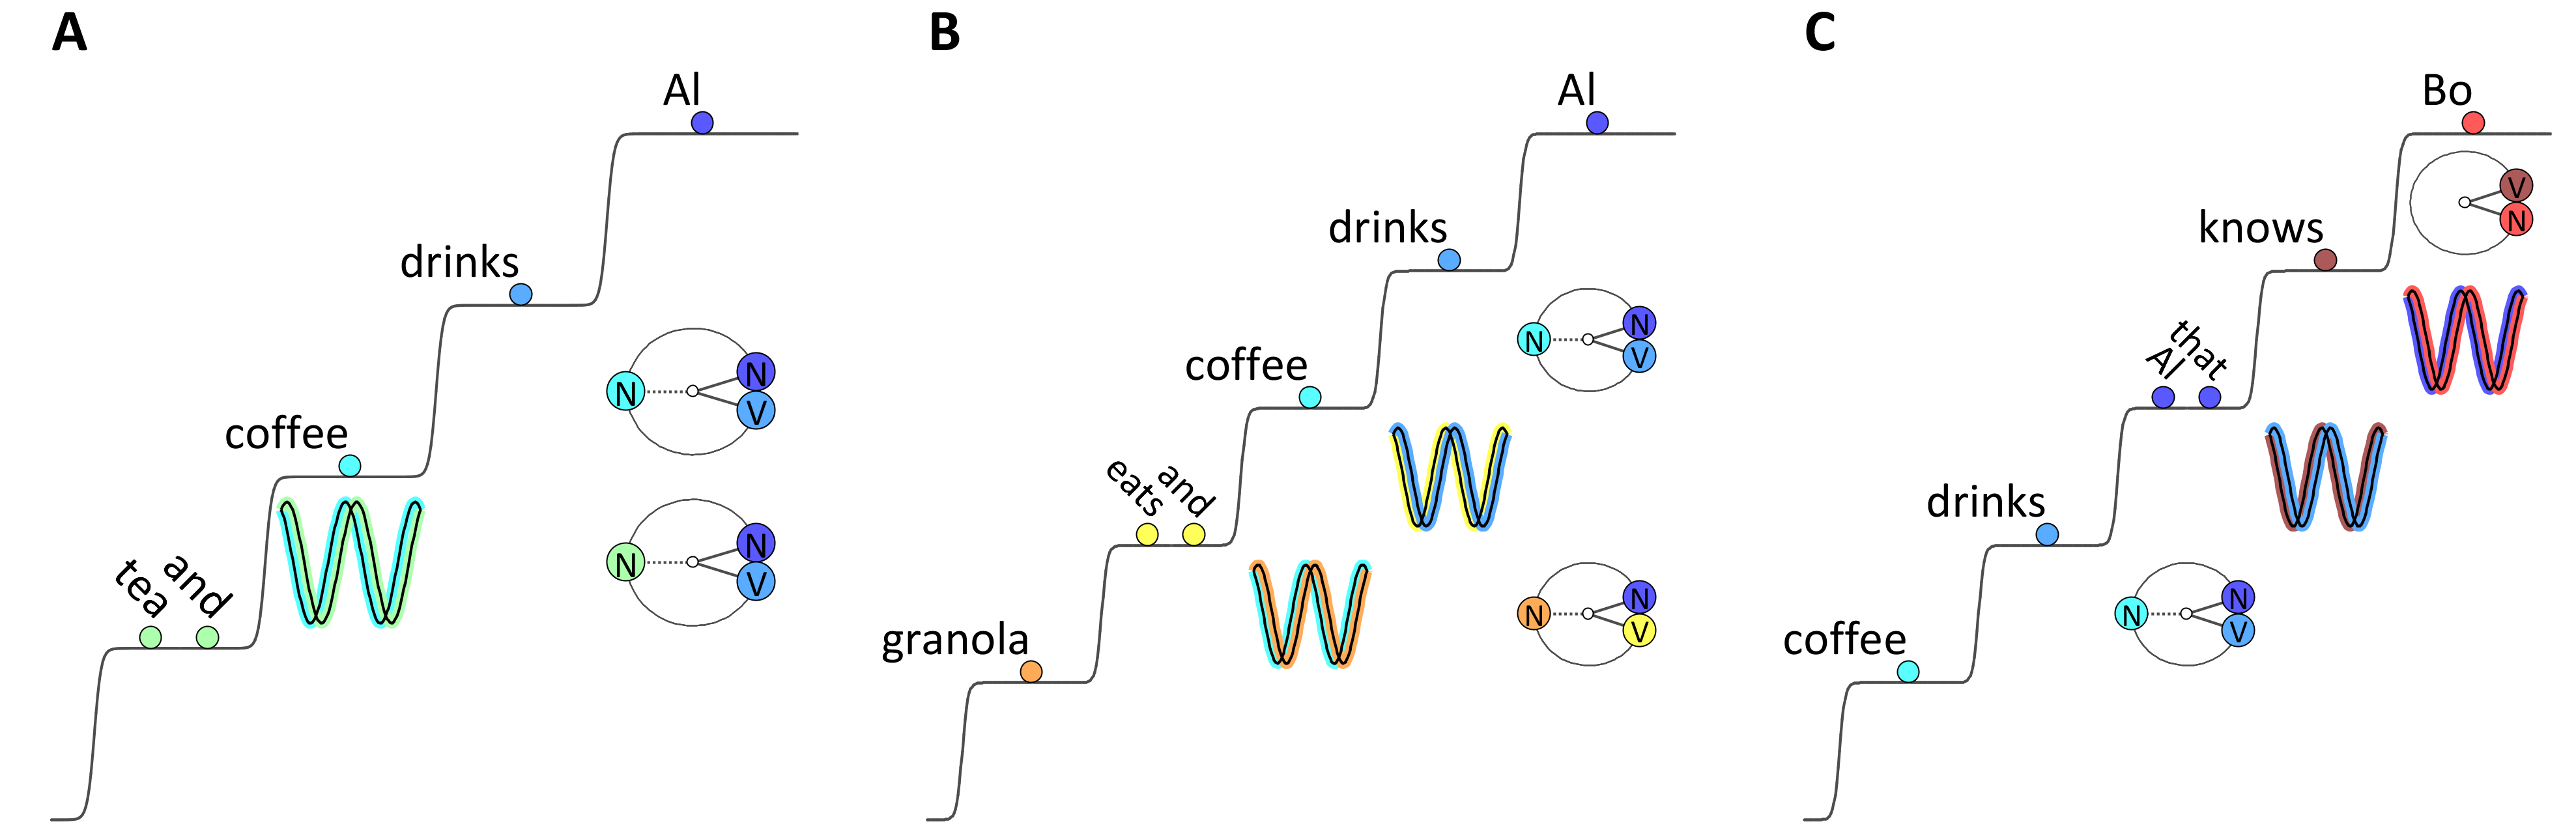
\includegraphics[width=\textwidth]{figures/Tilsen-img94.png}
\caption{\missingcaption}
\label{fig:4:44}
\end{figure}
 

  Given that coordination and subordination create interference, the critical question we must address is whether the interference is destabilizing? Can configurations with interference such as those above be stable? 

\subsection{Excitation asymmetries and modulation of coupling forces}

Interference is not necessarily destabilizing. The magnitude of interference depends on the relative \textit{e} values of the systems involved, because coupling force strengths depend on system \textit{e}. This follows from our microscopic model, where \textit{e} is correlated with population size and hence influences the number of synaptic projections between populations. When two asymmetrically excited c-systems induce differentiation interference in an s-system, the more highly excited cs-system has stronger destabilizing effect on the less highly excited one.

  To demonstrate macroscopically how excitation asymmetries mitigate against the adverse effects of interference, lets consider a toy example. Imagine two c-systems [c\textsubscript{1}] and [c\textsubscript{2}] which resonate with an s-system, \{s\}, which differentiates into subsystems \{s\textsubscript{1}\} and \{s\textsubscript{2}\}. Based on our standard hypotheses regarding c-s interactions and differentiation, we have the φ coupling matrix below, where φ\textsubscript{ij} is the strength of the force that system \textit{j} exerts on system \textit{i}. All coupling strengths are assumed to be proportional to source system excitations. We probe the φ stability patterns of the system under symmetric excitation (φ\textsubscript{ij} = φ\textsubscript{ji}) vs. asymmetric excitation (\textit{a}\textsubscript{1} > \textit{a}\textsubscript{2}, \textit{b}\textsubscript{1} > \textit{b}\textsubscript{2}, \textit{c}\textsubscript{21} > \textit{c}\textsubscript{12}). Note that \textit{c}\textsubscript{ij} in particular is the macroscopic manifestation of cc-s differentiation interference.

φ \textit{=} 


\begin{equation*}
% \begin{matrix}
% ?
% \begin{matrix}{c}_{1} & {c}_{2} & {s}_{1} & {s}_{2}\\
% {c}_{1}: & ?{a}_{1} & {c}_{2}:
% \end{matrix}
% {a}_{2}{s}_{1}:{b}_{1}{c}_{12}{s}_{2}:{b}_{2}{c}_{21}
% \end{matrix}
\end{equation*}
\todo{commented out equation}

  The phase equations for the system are shown below. Each system has an intrinsic frequency \textit{f}, and its instantaneous phase velocity is the sum of this intrinsic frequency and coupling forces. The \textit{f} of s\textsubscript{1} and s\textsubscript{2} are fixed at 8 Hz in all simulations, while c-system intrinsic frequencies are Gaussian randomly distributed with mean µ = 8 Hz and standard deviation σ = 1. The surroundings \textit{S} are assumed to exert a random, time-varying force on each system,  ${\epsilon} _{i}$. 

\begin{equation*}
% \begin{matrix}{\varphi} _{\mathit{ij}}\\
% \sin \\
% ?{-\Phi} _{\mathit{ij}}\\
% {\acute{{\theta} }}_{i}=\left[{2\mathit{\pi f}}_{i}+{\epsilon} _{i}\left(t\right)\right]+\sum _{j}\Box \end{matrix}
\end{equation*}
\todo{commented out equation}
  To assess stability statistically, we conduct 1000 simulations with random, uniformly distributed initial θ on the interval [-π, π]. The cs-resonance asymmetry \textit{a\textsubscript{i}} = 2\textit{b\textsubscript{i}} is imposed. Surroundings perturbations are modeled as a Gaussian random walk in a quadratic potential, where the fluctuations have standard deviation σ\textsubscript{S}:

\begin{equation*}
{\epsilon} _{i}\left(t+1\right)={\epsilon} _{i}\left(t\right)+N\left(0,{\sigma} _{S}\right)-{{\epsilon} _{i}\left(t\right)}^{2}
\end{equation*}
 

  By varying the coupling strengths \textit{c}\textsubscript{12} and \textit{c}\textsubscript{21},  we observe that the φ of cs\textsubscript{1} only stabilizes when \textit{c}\textsubscript{21} << 1, and vice versa, cs\textsubscript{2} only stabilizes when \textit{c}\textsubscript{21} << 1. In other words, only one of cs\textsubscript{1} and cs\textsubscript{2} can be stable and highly excited. Of course a variety of additional factors can also influence stability, such as the size of the surroundings fluctuations, and differences in intrinsic frequencies of c-systems. It also stands to reason that more differentiations should reduce stability of all but the most highly excited cs-resonance.

The model above shows how cc-s differentiation interference is manifested macroscopically and how excitation asymmetries can mitigate against interference, favoring stability for highly excited systems at the expense of less highly excited one. In order to arrive at this conclusion, a number of assumptions were made about the strengths of parameters and distributions of random variables. The toy model is limited in that excitation dynamics are implicit in coupling strength parameters. Incorporating explicit excitation dynamics doubtless brings further complications, but our presumption is that under fairly mild assumptions, the above conclusions regarding the destabilizing effects of interference will hold.

  The modulation of coupling forces by \textit{e} values suggests that a subset of excited, interfering systems could be stable, i.e. the subset which obtains higher levels of excitation. The waveform representations of interference below, in contrast to our previous ones, show interference as excitation-modulated. Given the above results, we can infer that interference between [Bo]\{+N\} and [Al]\{+N\} in the initial configuration does not destabilize the [Bo]\{+N\} system, because [Al]\{+N\} is not highly excited. Conversely, [Al]\{+N\} is destabilized because it experiences strong interference from [Bo]\{+N\}. Likewise, [knows]\{V\} can be stable,  but [drinks]\{V\} is more likely not to be stable. 

  Given that in the initial configuration [Al]\{+N\} and [drinks]\{V\} experience potentially destabilizing interference from more highly excited systems, the question arises whether we should prefer the representation in (A) or (B) below. If the configuration {\textbar}Al drinks coffee{\textbar} is stable and gives rise to a relational meaning experience at the same time as {\textbar}Bo knows{\textbar} does, then (A) is preferable because the relevant cs-systems of the {\textbar}Al drinks coffee{\textbar} configuration are above ground, a prerequisite for the experience. On the other hand, if {\textbar}Al drinks coffee{\textbar} is unstable, then no meaning experience arises (at least in those epochs in which {\textbar}Bo knows{\textbar} is excited), and thus (B) is preferable. (Gray-shading of systems is used to indicate their sub-excitation (ground) level state).

  
\begin{figure}
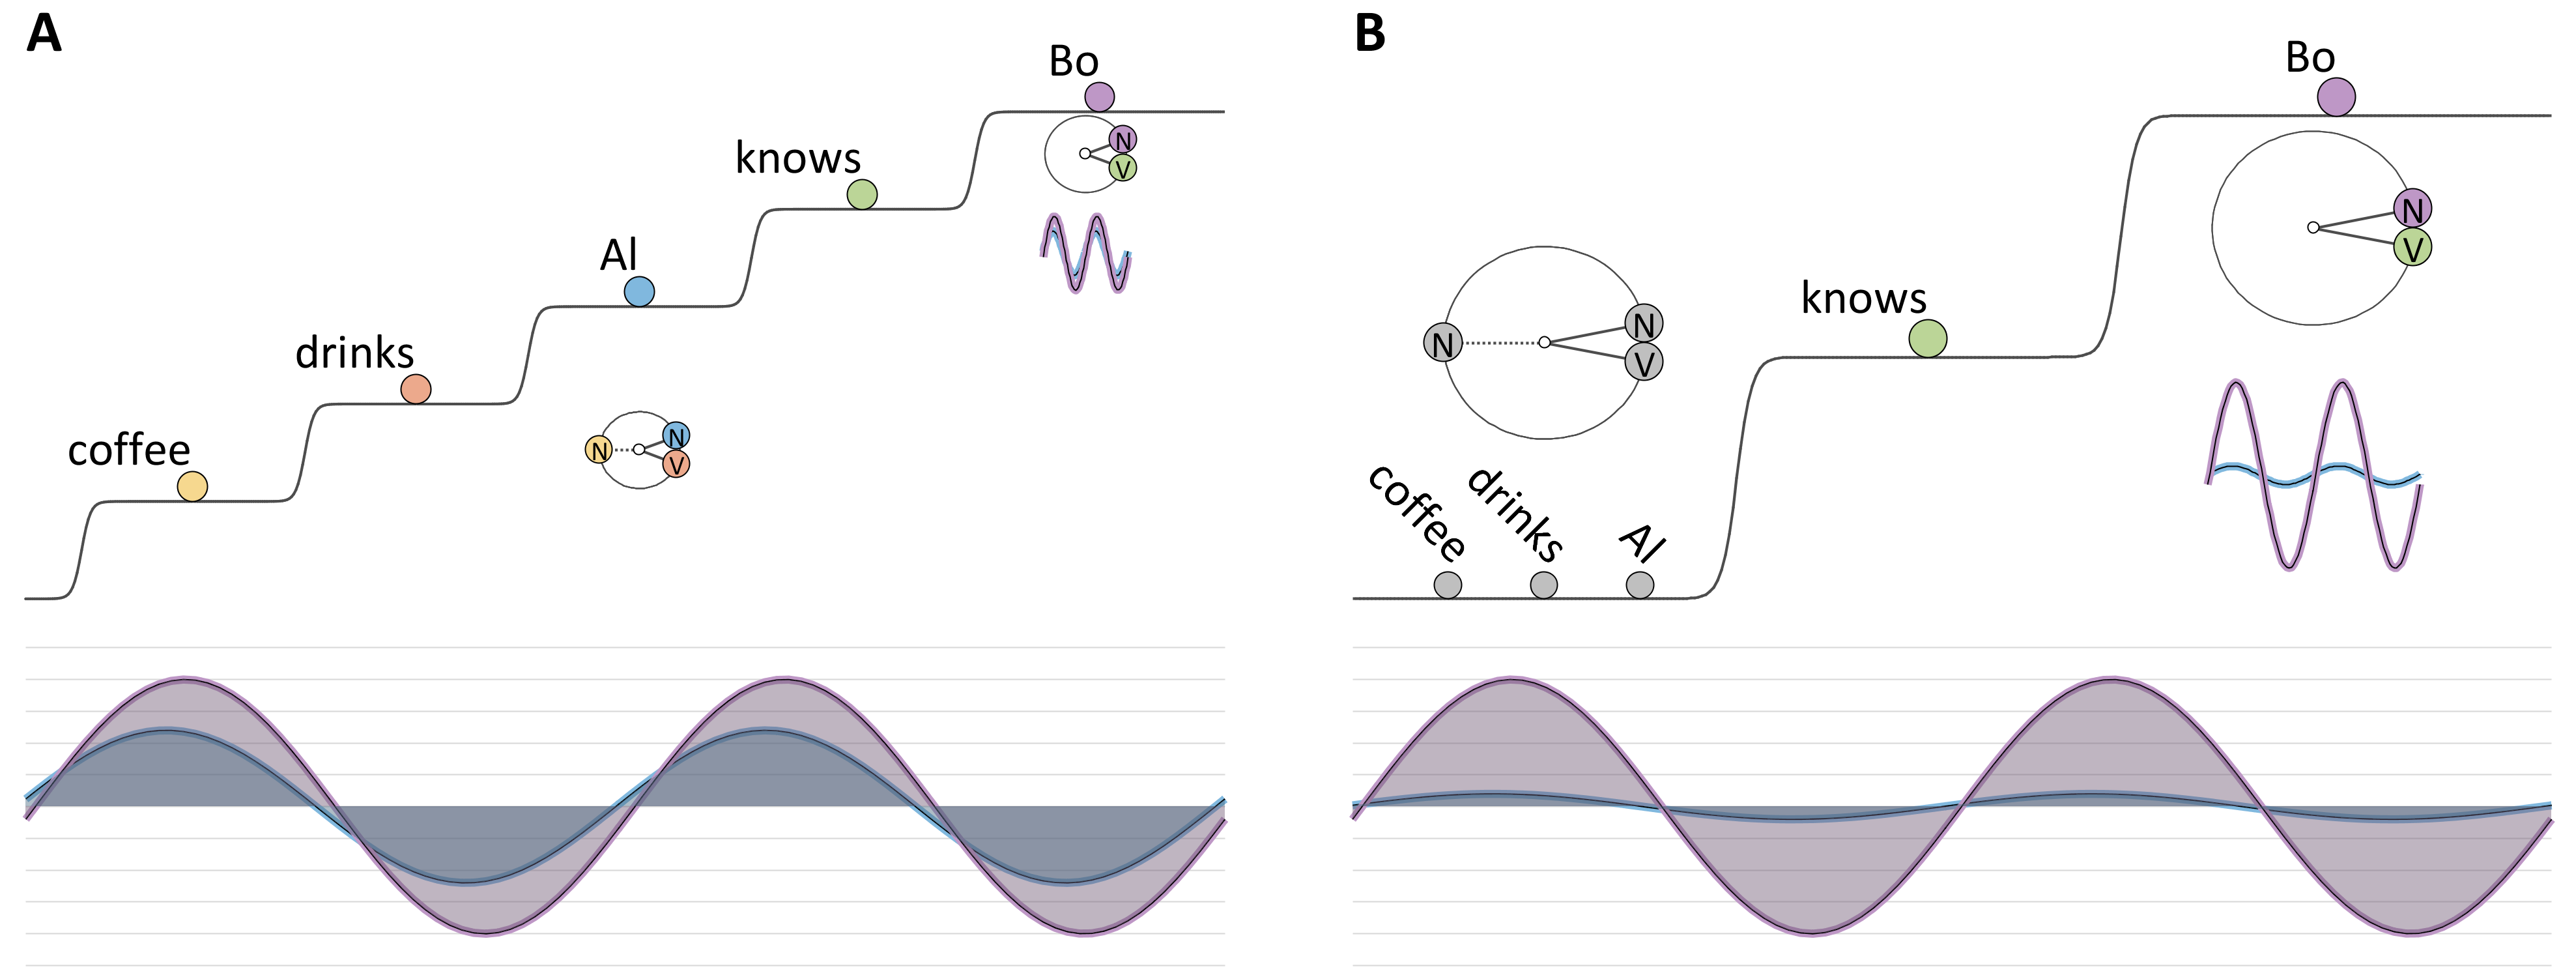
\includegraphics[width=\textwidth]{figures/Tilsen-img95.png}
\caption{\missingcaption}
\label{fig:4:45}
\end{figure}

   In some cases, it may be difficult to resolve between representations such as (A) and (B). It is relevant to note that the e-potentials we use do not entail specific values of e, only relative values. We often depict equidistant steps in both excitation (horizontal) and excitation potential (vertical) dimensions, but there is no a priori reason to impose linearity on the quantal organization. Below are three variations of initial e configurations of \textit{Bo knows Al drinks coffee}. In (A) potential differences between e-levels are nonlinear: potential levels closer to ground are more closely spaced. In (B) excitation differences are nonlinear: relative excitation values of systems with lower excitation are more closely spaced. In (C) both excitation potential and excitation values are nonlinearly spaced.

  
\begin{figure}
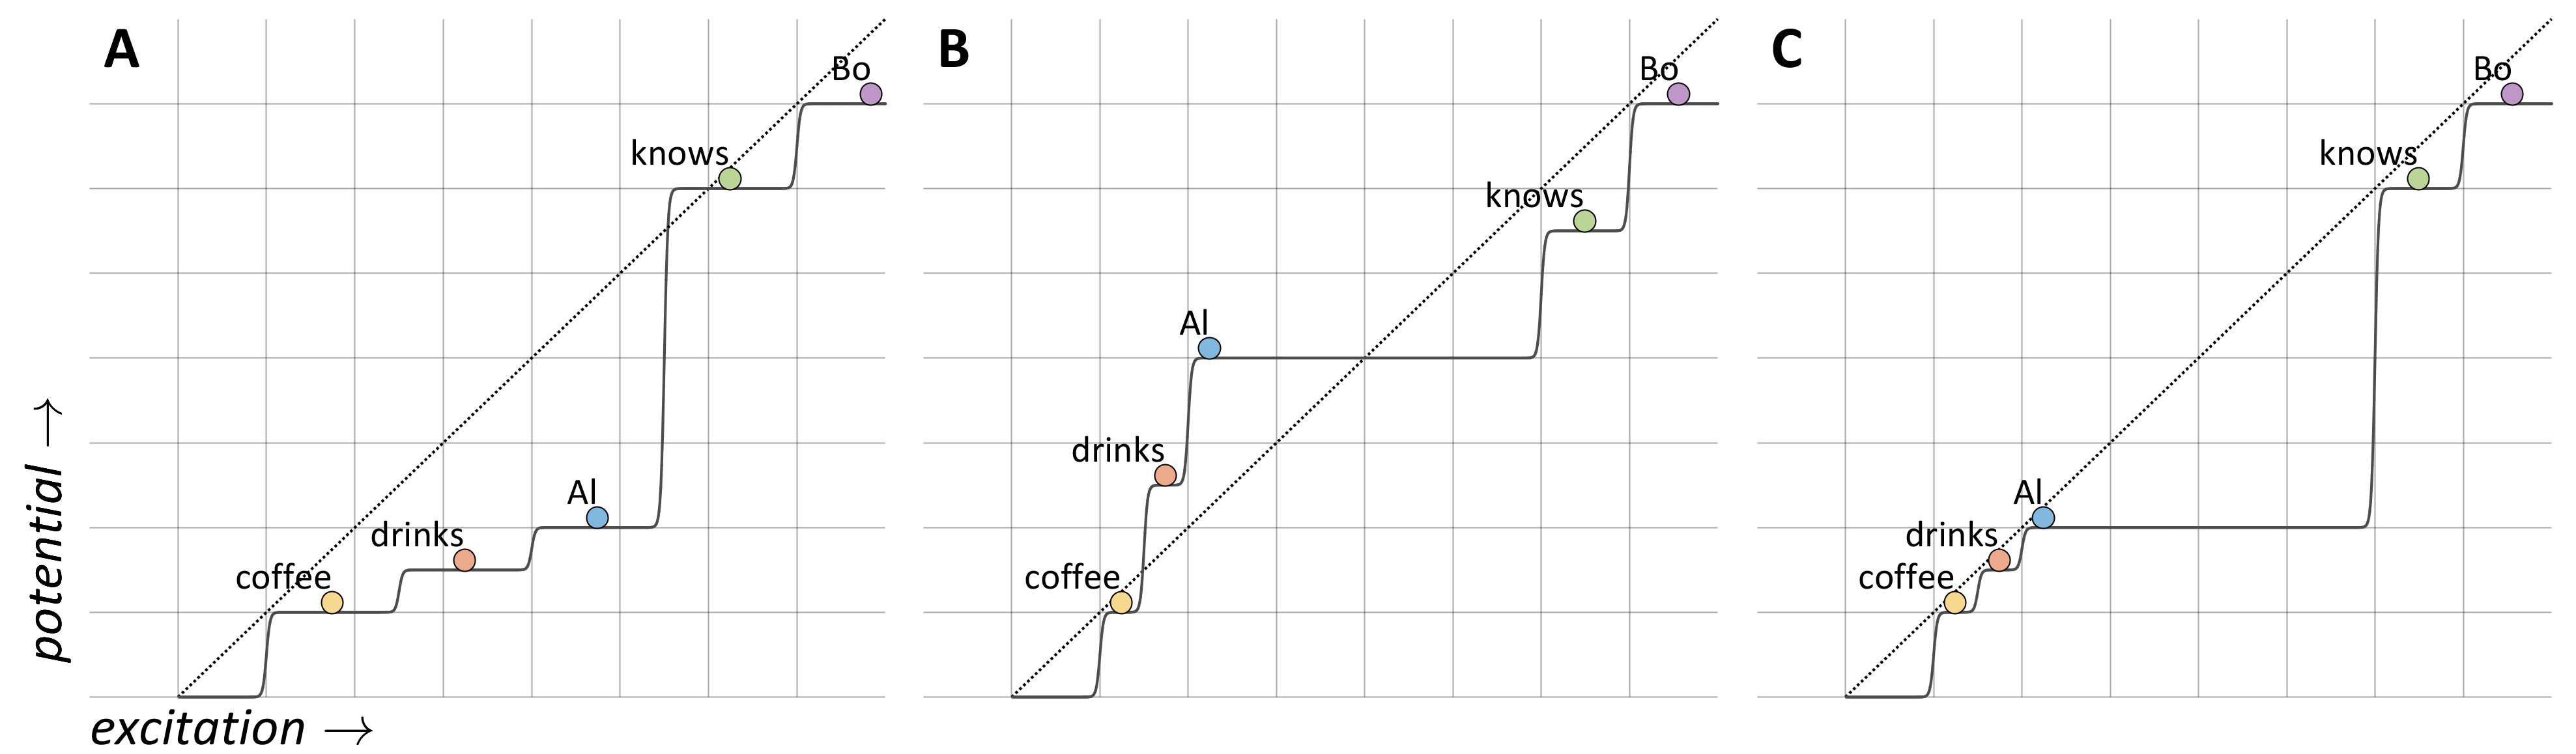
\includegraphics[width=\textwidth]{figures/Tilsen-img96.png}
\caption{\missingcaption}
\label{fig:4:46}
\end{figure}
   

  The nonlinear potentials provide a clearer picture of why excitation asymmetries are important for assessing the destabilizing effects of interference, and to some extent they help us see why the distinction between grounded/excited systems is not necessarily clear cut, particularly when there are only a couple of relevant φ configurations. We might very well experience {\textbar}Al drinks coffee{\textbar} during epochs when {\textbar}Bo knows{\textbar} is more highly excited, and vice versa, experience {\textbar}Bo knows{\textbar} during epochs in {\textbar}Al drinks coffee{\textbar} is more highly excited. This parallel experience of configurations corresponds to the trajectory in (A) below. On the other hand, it is also possible that the interference between configurations destabilizes the more weakly excited systems, in which case the configurations are not experienced in parallel, but in a sequence. This sequential attention to φ configurations corresponds to the trajectory in (B):

  
\begin{figure}
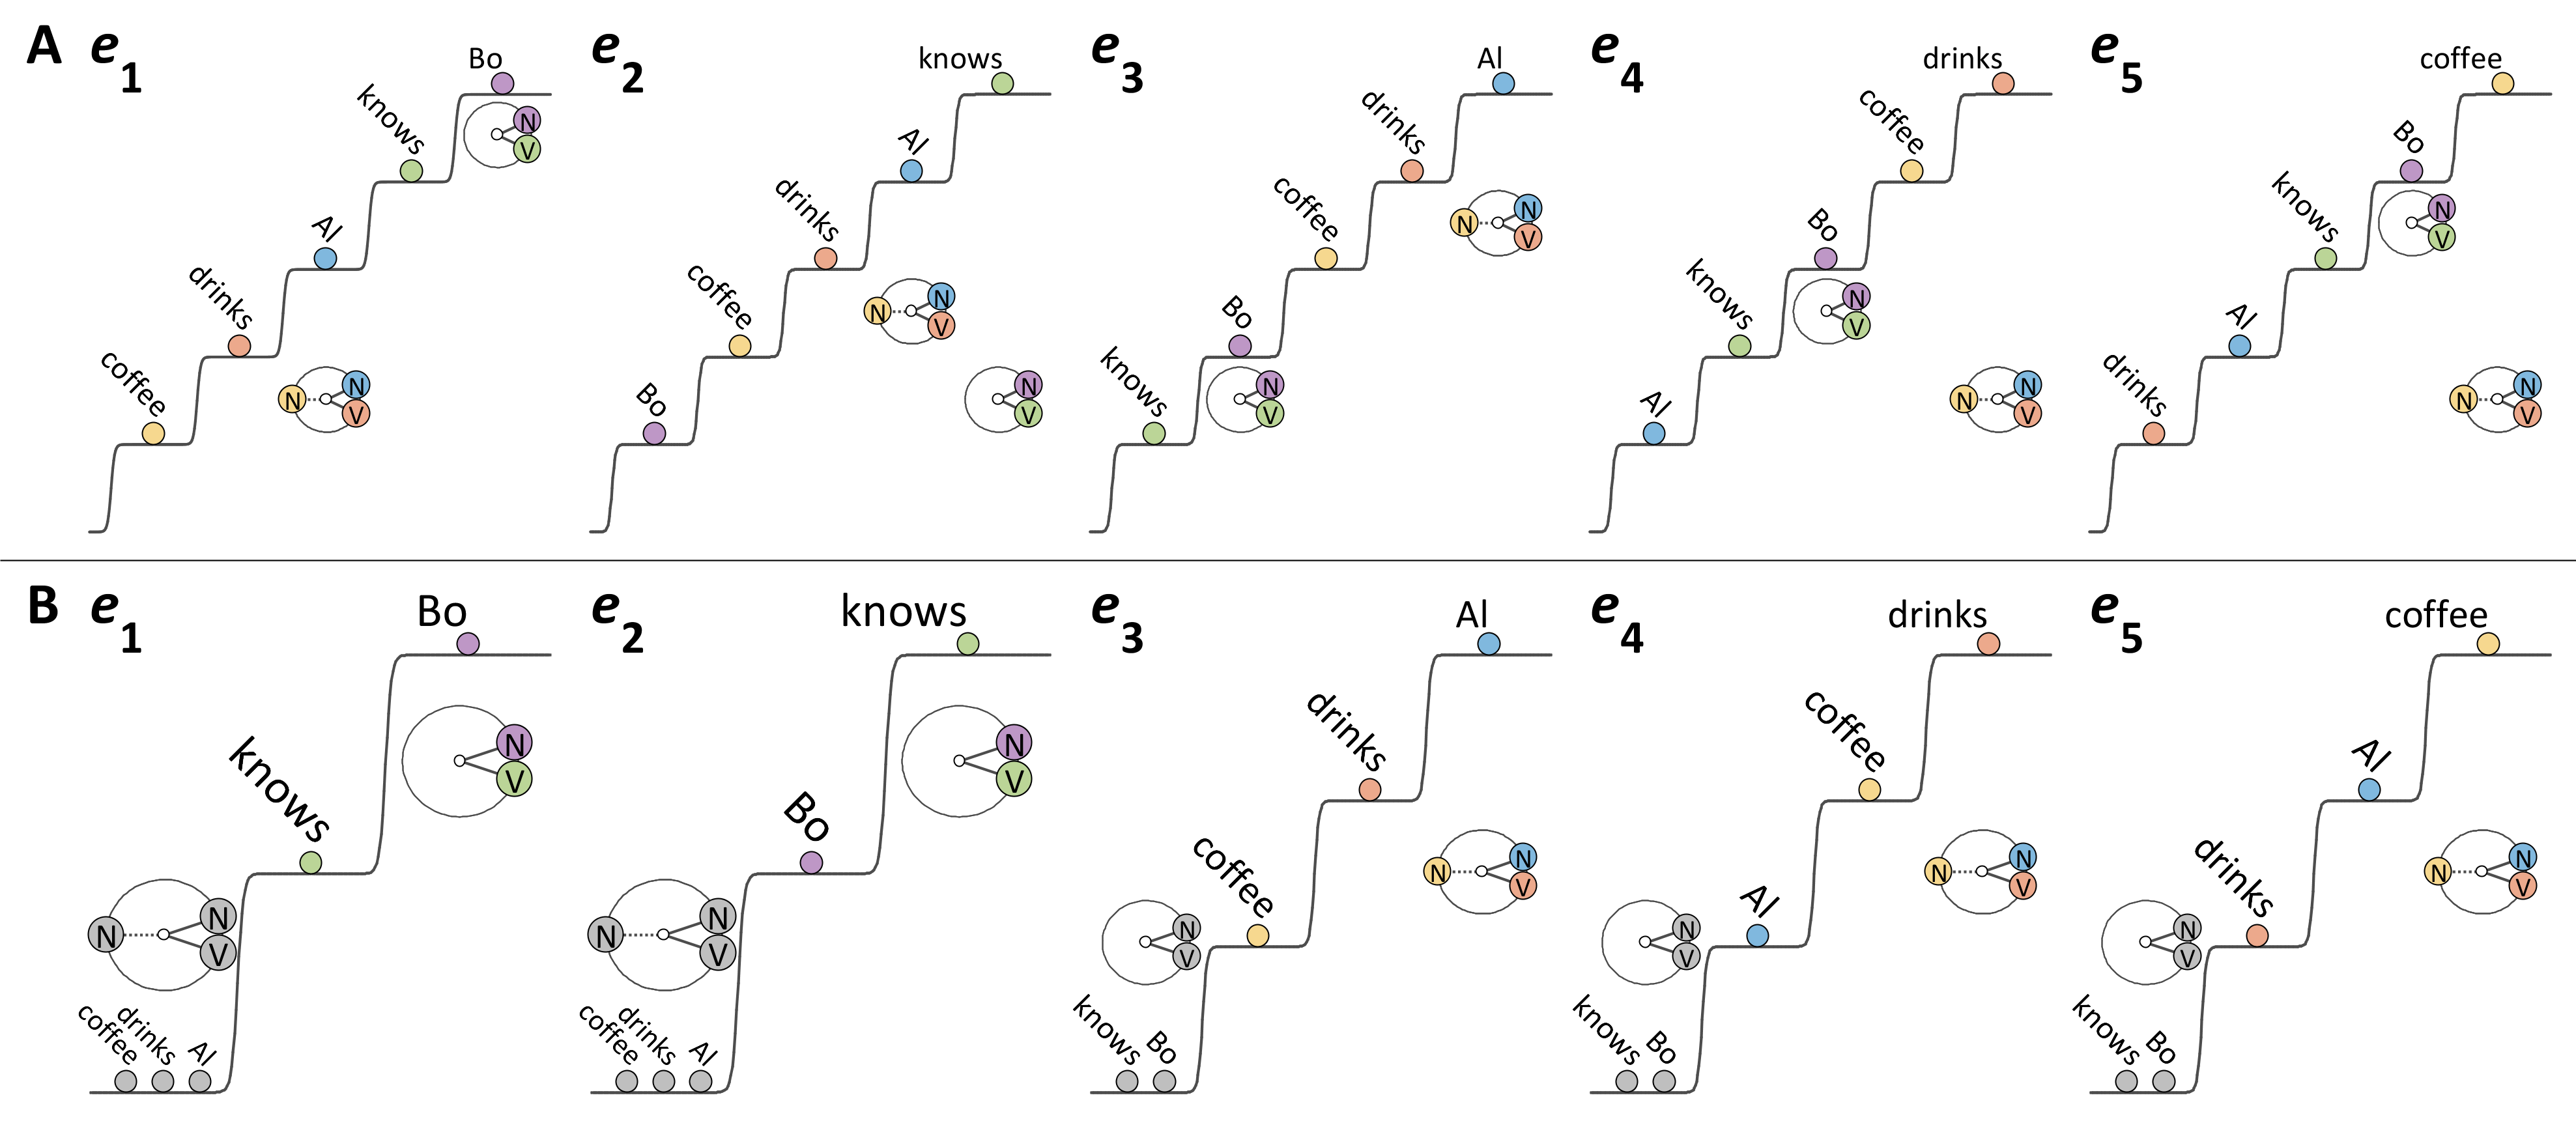
\includegraphics[width=\textwidth]{figures/Tilsen-img97.png}
\caption{\missingcaption}
\label{fig:4:47}
\end{figure}
 

  In longer utterances, with a greater number of interfering cs-systems, the likelihood that multiple configurations can simultaneously obtain an excited state must diminish. For example, in \textit{Al drinks coffee, tea, pop, beer, and whisky}, the systems [coffee], [tea], [pop], [beer], [whisky] require differentiation of \{-N\} into five subsystems. It seems unlikely that all of these systems can be \textit{simultaneously} stable and sufficiently excited to participate in a relational meaning experience, as implied by the initial organization in (A). The more sensible representation is (B), in which just one configuration is initially excited. In this analysis, attention is restricted in any given epoch to just a small set of φ configurations.

  
\begin{figure}
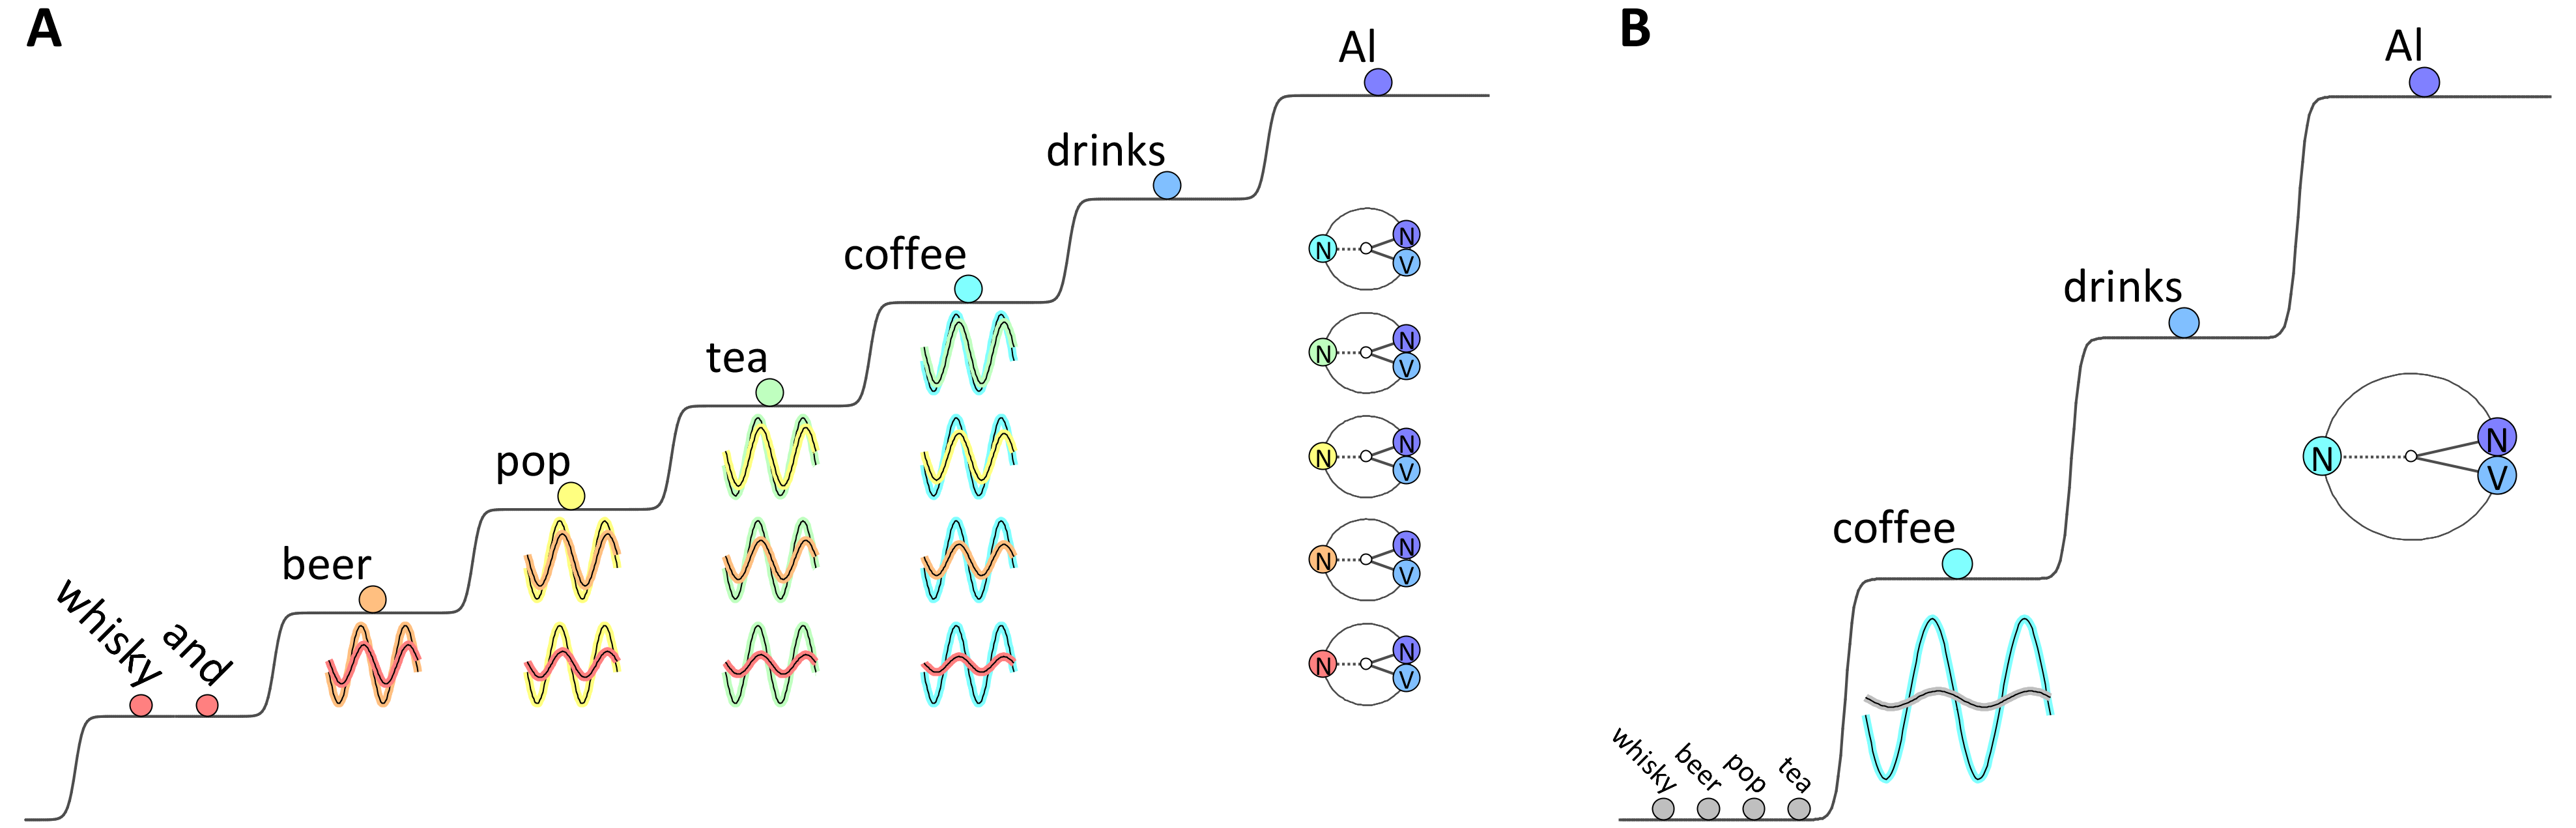
\includegraphics[width=\textwidth]{figures/Tilsen-img98.png}
\caption{\missingcaption}
\label{fig:4:48}
\end{figure}
 

  If we adopt the restricted-attention analysis of the initial configuration (B), then we cannot use the canonical reorganization operator Ê\textsuperscript{cr} to generate the production trajectory, because Ê\textsuperscript{cr} only operates on excited systems. To address this, we hypothesize a second type of reorganization, \textit{selective reorganization}.

\subsection{Attentionally selective reorganization}

Because of interference, only a small number of φ configurations can be excited in any given e-epoch. For an utterance with many relational meaning experiences, instead of imagining all configurations to be simultaneously excited, we imagine that only a subset are excited in any given e-epoch. In order for e-organization to achieve this, we hypothesize a \textit{selective reorganization} operator Ê\textsuperscript{sr}. The typical mapping of  Ê\textsuperscript{sr} is to demote previously selected system(s) to ground and promote some grounded system or set of grounded systems to selection level. For example, the selective reorganization operator maps (e3) to (e4) by grounding [coffee]\{N\} and ungrounding [tea]\{N\}. Likewise, the selective reorganization (e4) to (e5) grounds [tea] and ungrounds [whisky]. The advantage of selective reorganization is that in any given epoch, only cs-systems associated with the attended φ configuration are excited.

  
\begin{figure}
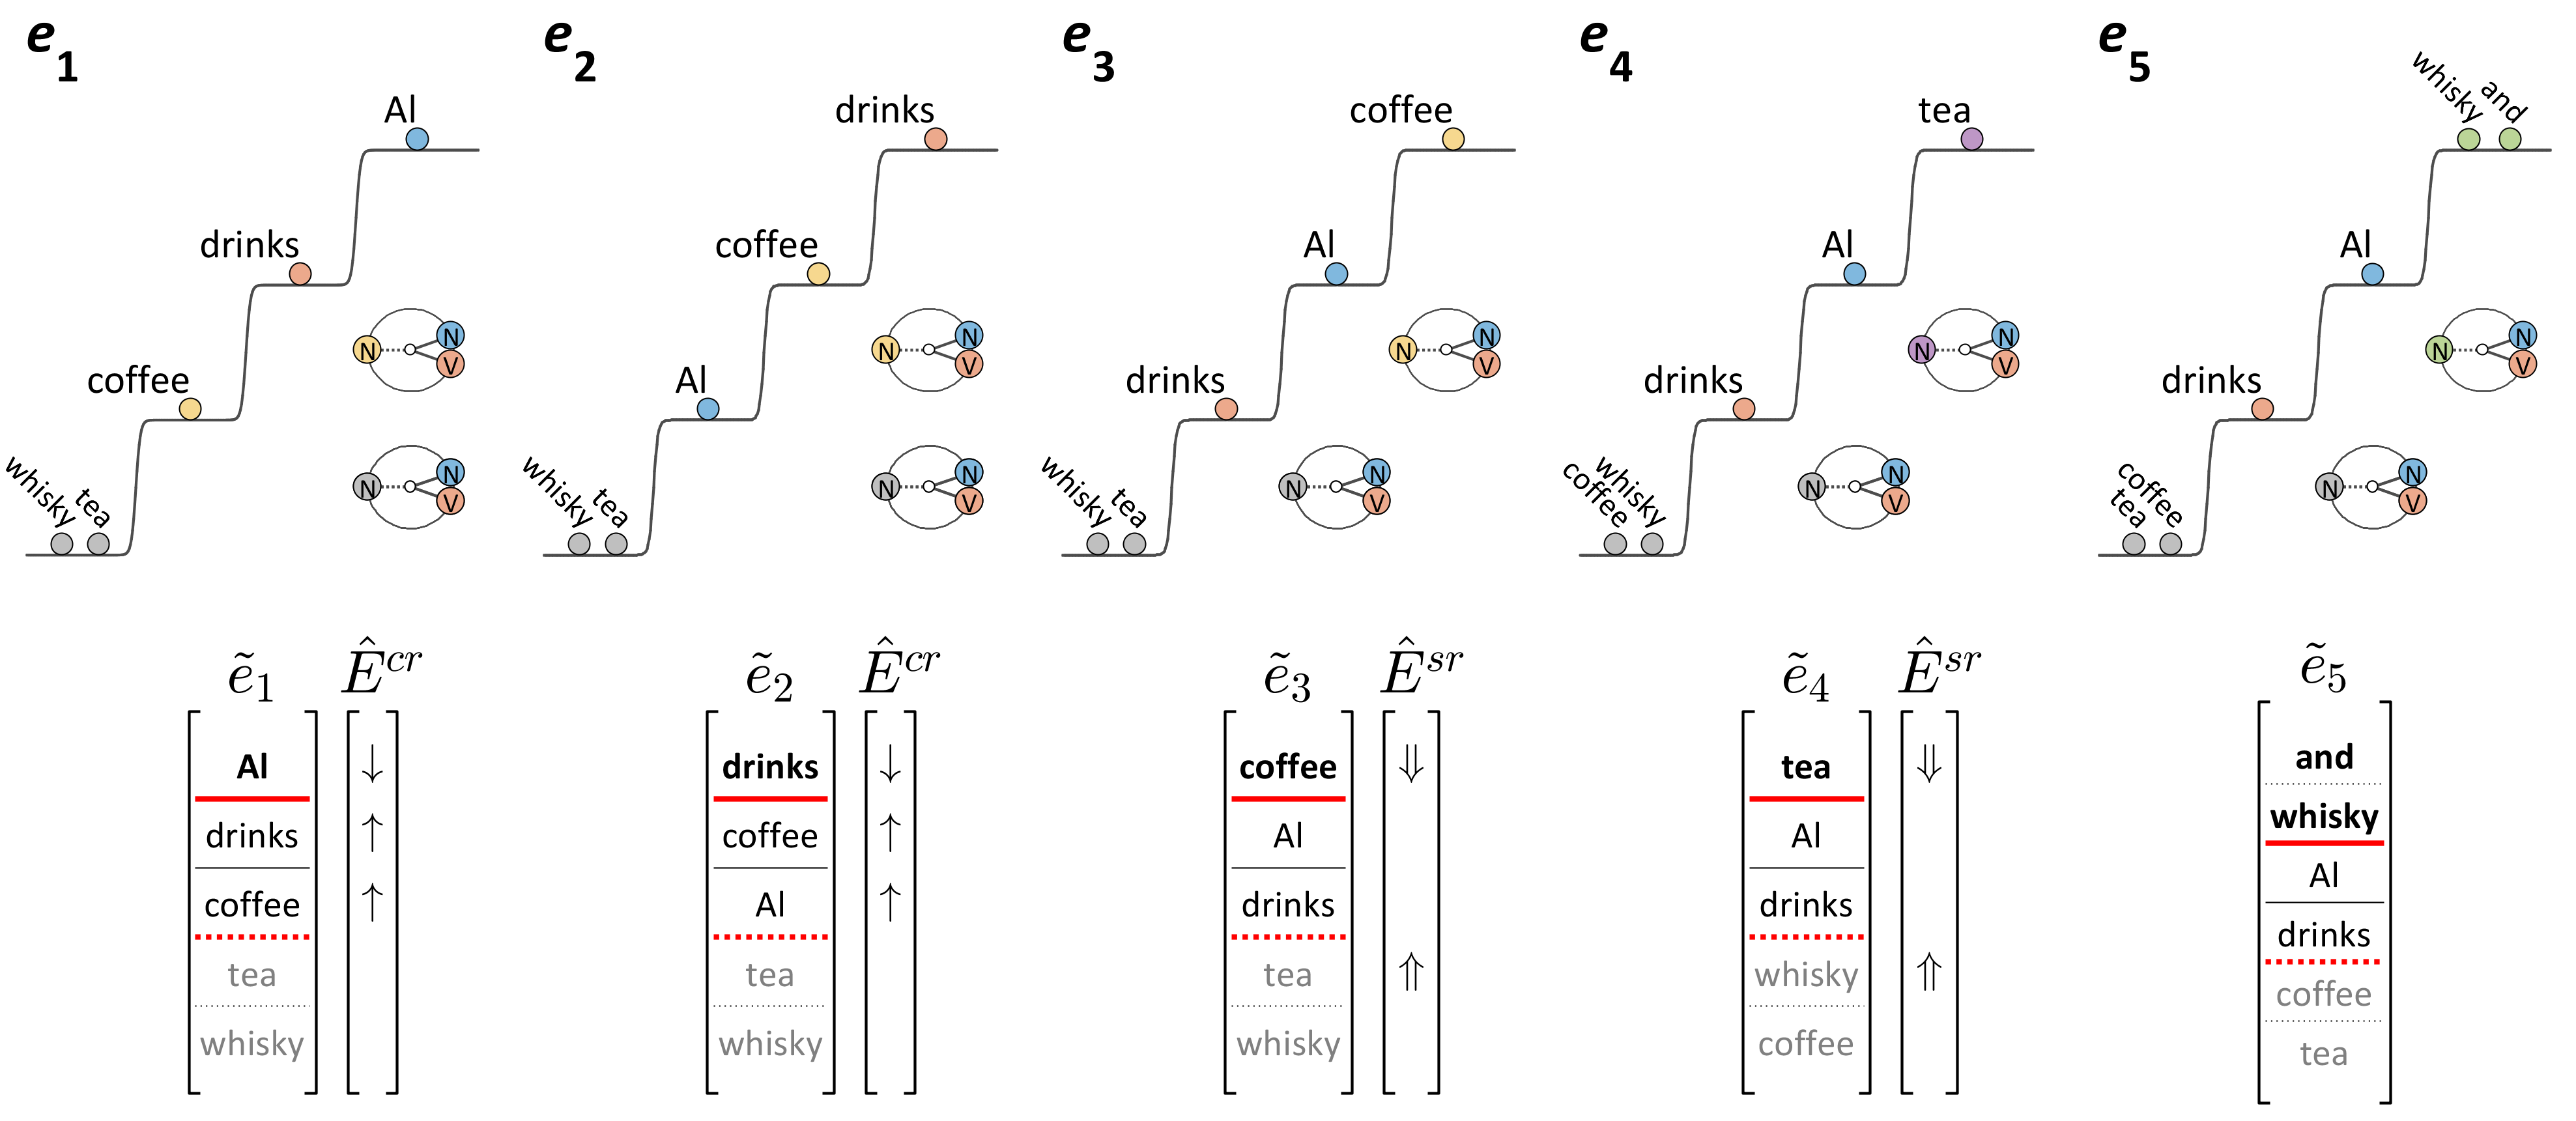
\includegraphics[width=\textwidth]{figures/Tilsen-img99.png}
\caption{\missingcaption}
\label{fig:4:49}
\end{figure}
   

  We sometimes refer to the selective reorganization operator as \textit{attentionally selective} reorganization, because each reorganization focuses attention on a subset of configurations from a larger set of active configurations. This is accomplished by a combination of grounding demotions and ungrounding promotions.

  One issue to consider for such analyses is how a particular order of items in a list can be maintained. For example, how does selective reorganization achieve the order \textit{…coffee, tea, and whisky} instead of \textit{…coffee, whisky, and tea}. One possibility is that there are differences in excitation values of the relevant ground-level systems, and the selective reorganization operator promotes ground-level system(s) according to their relative \textit{e} values. Yet there are probably limitations on how many systems can have distinct \textit{e} values at ground-level. Indeed, limitations on distinctions in \textit{e} at ground level predict that the items from long lists will not always be produced in a target order. For lists with many items, a long-term associative memory mechanism which is not yet incorporated in our conceptual model is necessary. This makes sense given that long lists must be learned through practice.

  The reader may have noticed that the above analysis of [and]\{\textsc{conj}\} departs in some ways from previous analyses. Instead of representing [and]\{\textsc{conj}\} as an excited system throughout the production, we treat it as a system which becomes active and excited when a selective reorganization occurs, often this is the last Ê\textsuperscript{sr} in a sequence. This reanalysis of \{\textsc{conj}\} gels with the observation that \{\textsc{conj}\} s-systems can be associated with each Ê\textsuperscript{sr}, as in \textit{Al drinks coffee and tea and whisky and…} Furthermore, \{\textsc{conj}\} can also fail to be selected altogether, as in \textit{Al drinks coffee, tea, whisky}.

  Attentionally selective reorganization can be generalized readily to other varieties of coordination. For example, in the verb phrase coordination \textit{Al drinks coffee and eats granola}, we imagine as below that after selection of [coffee]\{-N\} in (e3) a selective reorganization promotes both [eats]\{V\} and [granola]\{-N\} while grounding [drinks]\{V\} and [coffee]\{-N\} (e4). Only [Al]\{+N\} persists in an excited state in the selective reorganization. The propensity of [Al]\{+N\} to persist in this case can be seen as a consequence of the fact that no alternative \{+N\} system is promoted in the selective reorganization.

  
\begin{figure}
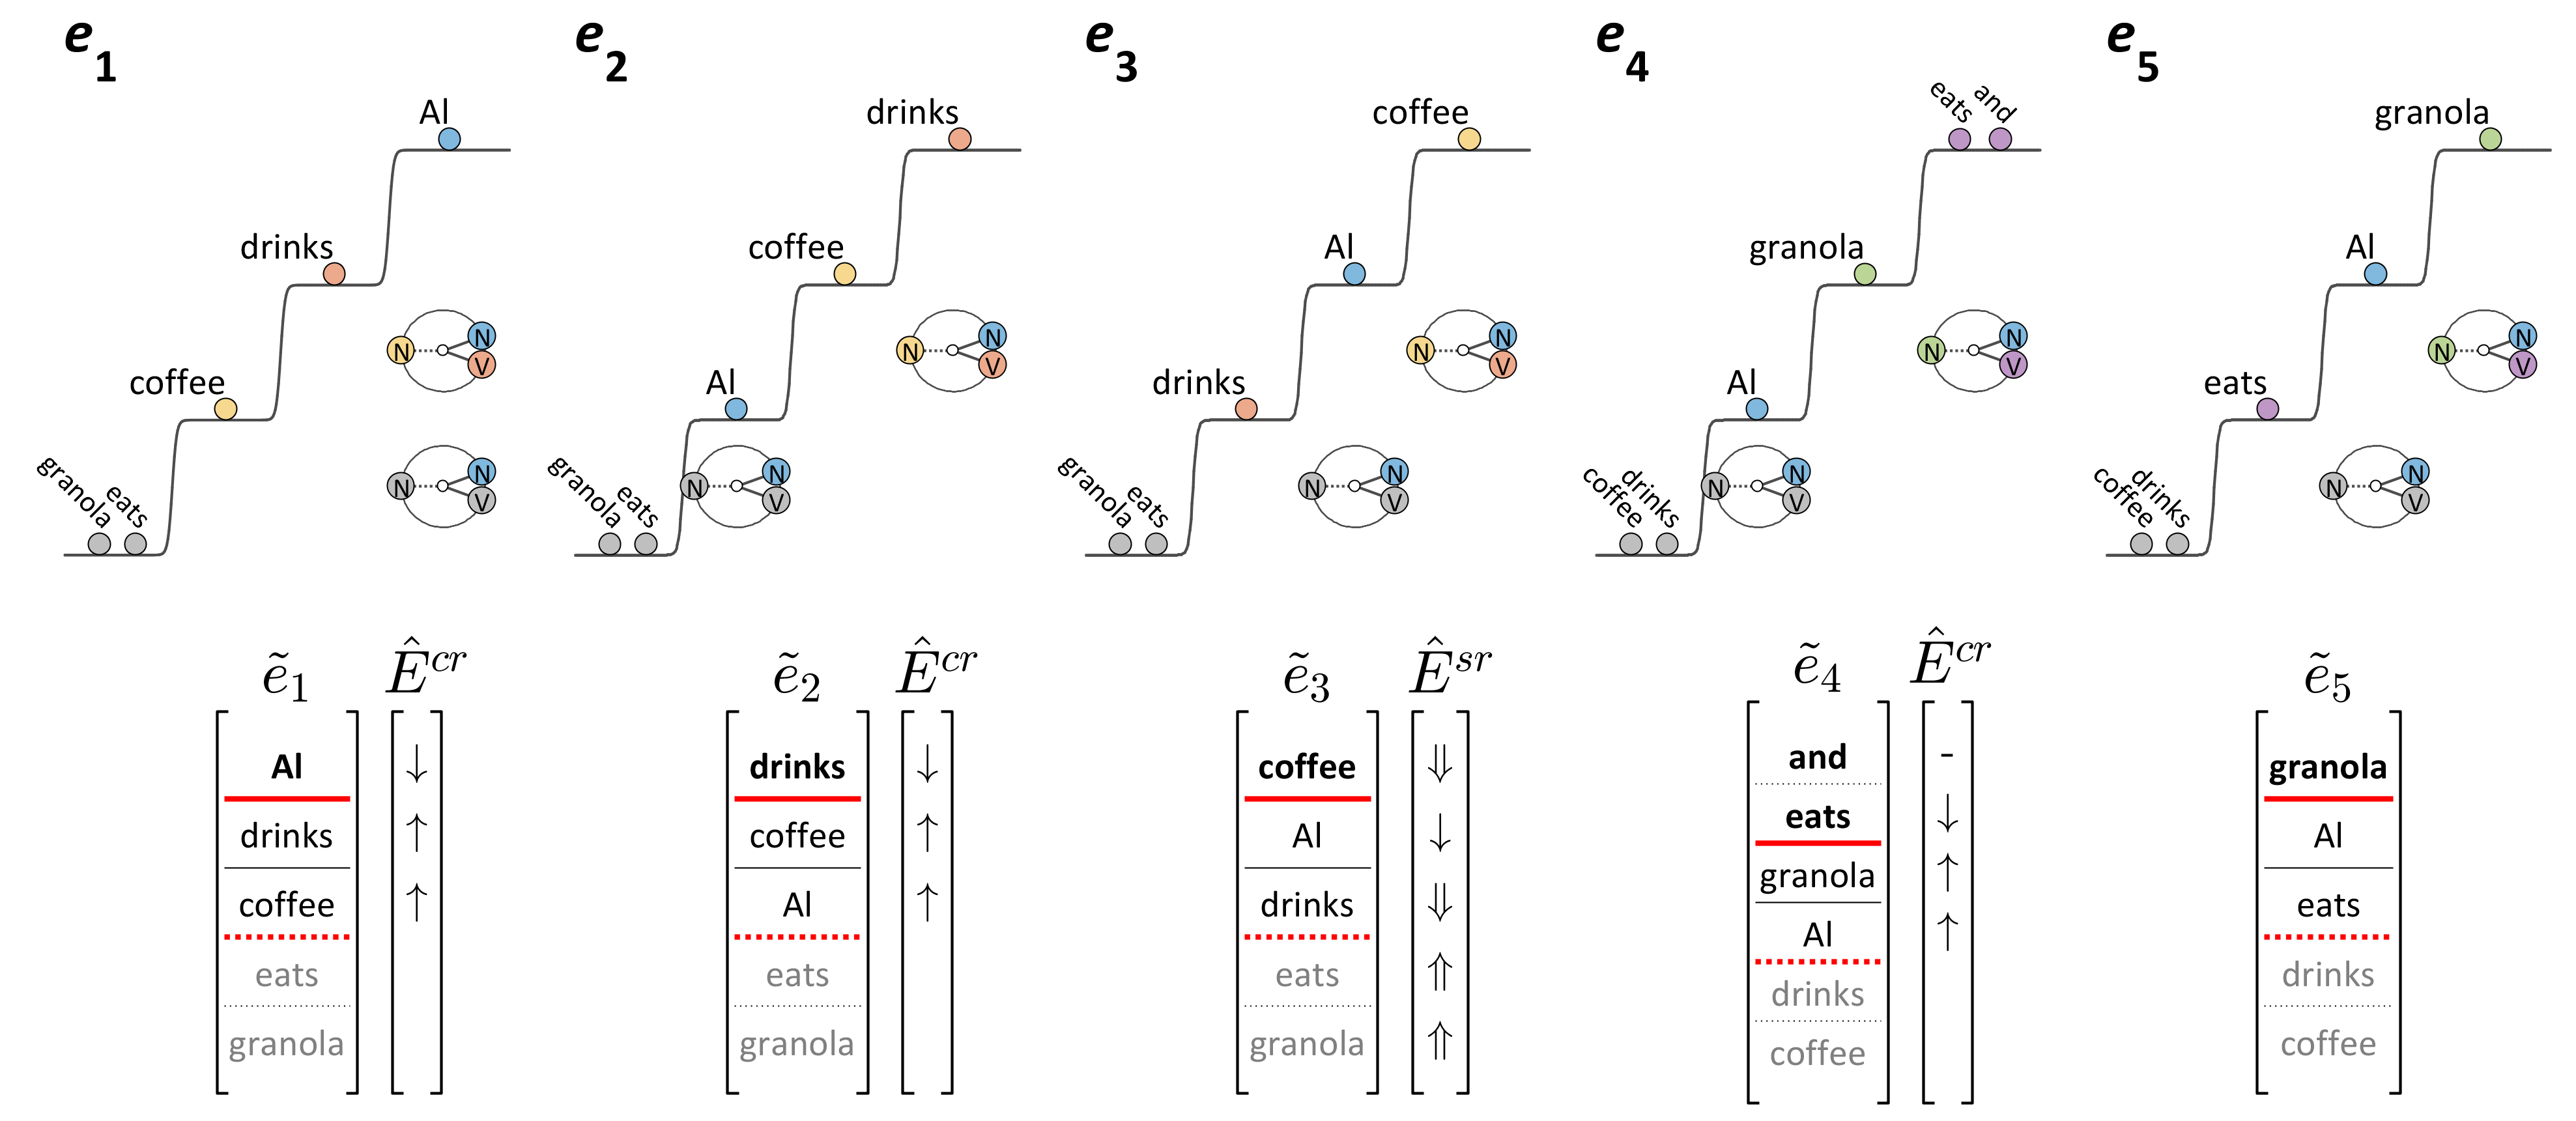
\includegraphics[width=\textwidth]{figures/Tilsen-img100.png}
\caption{\missingcaption}
\label{fig:4:50}
\end{figure}
 

  We can further generalize selective reorganization to complement clauses, as in \textit{Bo knows that Al drinks coffee}, shown below. Note that we analyze [that]\{C\} similarly to [and]\{\textsc{conj}\}: [that]\{C\} is activated and excited to selection level in conjunction with a particular selective reorganization, and it is deactivated in the subsequent reorganization. 

  
\begin{figure}
\includegraphics[width=\textwidth]{figures/Tilsen-img101.png}
\caption{\missingcaption}
\label{fig:4:51}
\end{figure}
 

  Because of interference and stability considerations, there must be limits on how many systems can be promoted from ground-level in a selective reorganization. In many circumstances, these limits appear to correspond to configurations that are conventionally described as a single clause or adjunct phrase.

  Another application of selective reorganization involves relative clauses. Object- and subject- relative clauses are shown below. In both cases, we analyze relative clauses with a relative cs-system [\textsc{rel}]\{R\} that is +φ-coupled to a main clause cs-system and also participates in a φ configuration with a subordinate clause \{V\}. In the object relative, \textit{Al drinks coffee which Bo brews}, [which]\{R\} is +φ coupled to [coffee]\{-N\} and -φ coupled to [brews]\{V\}. This creates the {\textbar}Bo brews coffee{\textbar} configuration indirectly. In the subject relative, \textit{Al, who Bo knows, drinks coffee}, [who]\{R\} is +φ coupled to [Al]\{+N\} and -φ coupled to [knows]\{V\}. The {\textbar}Bo knows Al{\textbar} configuration is indirectly created by these relations.

  
\begin{figure}
\includegraphics[width=\textwidth]{figures/Tilsen-img102.png}
\caption{\missingcaption}
\label{fig:4:52}
\end{figure}
 

  
\begin{figure}
\includegraphics[width=\textwidth]{figures/Tilsen-img103.png}
\caption{\missingcaption}
\label{fig:4:53}
\end{figure}
 

  In both subject and object relatives, the excitation of the \{R\} system prevents the relativized main clause cs-system to which it is coupled from being demoted to ground. Thus in the object relative, the selective reorganization to (e4) that excites [which]\{R\} maintains [coffee]\{-N\} in an excited state. Likewise, in the subject relative, the selective reorganization to (e2) maintains [Al]\{+N\} in an excited state. In a sense, the excitation of \{R\} assists the persistence of excitation of a system which participates in another clausal φ configuration and which might otherwise be demoted to ground. We will encounter the phenomenon of assisted persistence of excitation in other contexts later on.

Attentionally selective reorganization allows for a radical reconceptualization of system trajectories in production.  Only a handful of systems are excited in any given stable epoch of a trajectory, while many more may be active. If too many cs-systems are excited and interfere, the state is likely to be unstable. We refer to the set of excited c-systems as the \textit{attentional focus}, or the \textit{attended configuration}, and all unexcited systems as \textit{unattended} systems. The implication is that when we produce or interpret a multi-clausal utterance (e.g. \textit{Al drinks coffee and eats granola}) we do not experience both clausal relational meanings uniformly in time; rather, we experience one relational meaning more strongly, and then the other.

  In this new conception, producers and interpreters \textit{do} have the ability to experience multiple relational meanings simultaneously, but those experiences are not equivalent. Only a limited set of the relational meanings can be sufficiently excited to be attentionally focused. For this new conception to be consistent with our understanding of e-organization, a more powerful version of the reorganization operator, Ê\textsuperscript{sr},  is needed. Selective reorganization gives even more importance to the distinction between excited states and the ground state. Whereas Ê\textsuperscript{cr} operates on systems in an excited state, Ê\textsuperscript{sr} alters the excited/unexcited states of systems. Later on we will find that this more powerful mechanism is not wholly unconstrained and helps us understand a variety of non-local phenomena; these include interactions of ellipsis and anaphora with coordination and subordination, as well as island effects. Ê\textsuperscript{sr} is somewhat more phenomenological than Ê\textsuperscript{cr}—the mappings of Ê\textsuperscript{sr} are not derived simply from feedback-induced suppression of a selected system. Nonetheless, a justification for Ê\textsuperscript{sr} can be made on the basis of its utility.

  A deeper rationale for our new conception of attentionally selective reorganization is that we can understand how instability from interference is avoided by focusing attention on a small number of configurations.  For an utterance with an arbitrarily long list, such as \textit{Al drinks coffee, tea, juice, water, pop, whisky, beer, cider, scotch}, etc., attentionally selective reorganization solves the multiplicity problem: there is no need to proliferate N units as in the connected objects representation: 

  
\begin{figure}
\includegraphics[width=\textwidth]{figures/Tilsen-img104.png}
\caption{\missingcaption}
\label{fig:4:54}
\end{figure}
 

  The multiplicity problem is avoided because we abandon the notion that all of the meaning relations are experienced in an equivalent way simultaneously. Connected object representations provide the impression that all objects are equally co-present and similarly related in space and time. Because we can now see this as misleading, the o/el paradigm requires that we reinterpret the conventional notions of “infinity” and “recursion”.

